

%% AAPT Physics Bowl Exams Questions
%%----------------------------------------

%% this file contains 823 problems

%http://www.aapt.org/Programs/PhysicsBowl/printexams.cfm
%http://www.aapt.org/Programs/PhysicsBowl/examconv.cfm

%% NOTE: think of a way to move tabulary to options!!


%% PhysicsBowl 2015 Division 01 only
%%----------------------------------------
\element{aapt}{ %% Bowl-M1
\begin{question}{bowl-2015-q01}
    Which one of the following choices correctly represents a length of \SI{3.00}{\milli\meter}?
    \begin{multicols}{2}
    \begin{choices}
        \wrongchoice{\SI{3.00e-6}{\meter}}
      \correctchoice{\SI{3.00e-3}{\meter}}
        \wrongchoice{\SI{3.00e-2}{\meter}}
        \wrongchoice{\SI{3.00e3}{\meter}}
        \wrongchoice{\SI{3.00e6}{\meter}}
    \end{choices}
    \end{multicols}
\end{question}
}

\element{aapt}{ %% Bowl-A1
\begin{question}{bowl-2015-q02}
    A box uniformly slides \SI{7.50}{\meter} to rest across
        a flat surface in a time of \SI{12.0}{\second}.
    What was the initial speed of the box when it started its slide?
    \begin{multicols}{2}
    \begin{choices}
        \wrongchoice{\SI{0.313}{\meter\per\second}}
        \wrongchoice{\SI{0.625}{\meter\per\second}}
      \correctchoice{\SI{1.25}{\meter\per\second}}
        \wrongchoice{\SI{2.50}{\meter\per\second}}
        \wrongchoice{\SI{5.00}{\meter\per\second}}
    \end{choices}
    \end{multicols}
\end{question}
}

\element{aapt}{ %% Bowl-A5
\begin{question}{bowl-2015-q03}
    Which one of the following quantities is not a vector quantity?
    \begin{multicols}{2}
    \begin{choices}
      \correctchoice{Average speed}
        \wrongchoice{Average velocity}
        \wrongchoice{Linear momentum}
        \wrongchoice{Acceleration}
        \wrongchoice{Average force}
    \end{choices}
    \end{multicols}
\end{question}
}

\element{aapt}{ %% Bowl-B1
\begin{question}{bowl-2015-q04}
    A standing wave on a string is produced.
    Which one of the following choices best describes the location
        on the string at which maximum constructive interference occurs?
    \begin{multicols}{2}
    \begin{choices}
        \wrongchoice{node}
      \correctchoice{antinode}
        \wrongchoice{harmonic}
        \wrongchoice{overtone}
        \wrongchoice{amplitude}
    \end{choices}
    \end{multicols}
\end{question}
}

\element{aapt}{ %% Bowl-A2
\begin{question}{bowl-2015-q05}
    An object initially is moving upward while in free fall.
    Which one of the following choices best represents the direction of the object's acceleration during its flight?
    \begin{center}
    \begin{tabu}{cX[c]X[c]X[c]}
        \toprule
        \makebox[1.5em][c]{\textnumero}
            & Object moving upward & Object at peak of motion & Object moving downward \\
        \bottomrule
    \end{tabu}
    \end{center}
    \begin{choices}
        \wrongchoice{\begin{tabu}{X[c]X[c]X[c]} Upward & Zero & Downward \\ \end{tabu}}
        \wrongchoice{\begin{tabu}{X[c]X[c]X[c]} Downward & Zero & Downward \\ \end{tabu}}
        \wrongchoice{\begin{tabu}{X[c]X[c]X[c]} Upward & Downward & Downward \\ \end{tabu}}
        \wrongchoice{\begin{tabu}{X[c]X[c]X[c]} Downward & Zero & Upward \\ \end{tabu}}
      \correctchoice{\begin{tabu}{X[c]X[c]X[c]} Downward & Downward & Downward \\ \end{tabu}}
    \end{choices}
\end{question}
}

\element{aapt}{ %% Bowl-A1
\begin{question}{bowl-2015-q06}
    A car travels at \SI{20.0}{\mile\per\hour}.
    Which one of the following choices best represents the speed
        of the car in SI units of meter per second (\si{\meter\per\second})?
    \begin{multicols}{3}
    \begin{choices}
        \wrongchoice{\SI{533}{\meter\per\second}}
        \wrongchoice{\SI{45.0}{\meter\per\second}}
        \wrongchoice{\SI{20.0}{\meter\per\second}}
      \correctchoice{\SI{8.9}{\meter\per\second}}
        \wrongchoice{\SI{0.75}{\meter\per\second}}
    \end{choices}
    \end{multicols}
\end{question}
}

\element{aapt}{ %% Bowl-A2
\begin{question}{bowl-2015-q07}
    An object moves clockwise with constant speed around the vertical circle shown.
    \begin{center}
    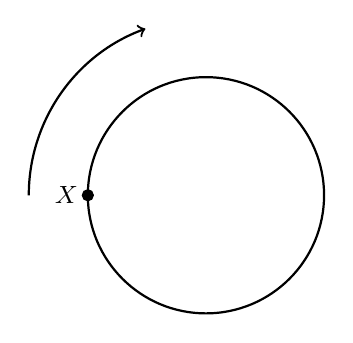
\begin{tikzpicture}[font=\small]
        \draw[thick] (0,0) circle (1.5cm);
        \draw[fill] (-1.5,0) circle (2pt) node[anchor=east] {$X$};
        \draw[thick,->] (-2.25,0) arc (180:110:2.25cm);
    \end{tikzpicture}
    \end{center}
    Which arrow best indicates the direction of the object's
        instantaneous acceleration at the point labeled $X$?
    \begin{multicols}{3}
    \begin{choices}
        \AMCboxDimensions{down=-0.33cm}
        \correctchoice{
            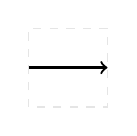
\begin{tikzpicture}
                \draw[white!90!black,dashed] (0,0) rectangle (1,1);
                \draw[thick,->] (0,0.5) -- (1,0.5);
            \end{tikzpicture}
        }
        \wrongchoice{
            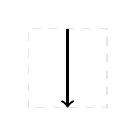
\begin{tikzpicture}
                \draw[white!90!black,dashed] (0,0) rectangle (1,1);
                \draw[thick,->] (0.5,1) -- (0.5,0);
            \end{tikzpicture}
        }
        \wrongchoice{
            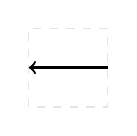
\begin{tikzpicture}
                \draw[white!90!black,dashed] (0,0) rectangle (1,1);
                \draw[thick,->] (1,0.5) -- (0,0.5);
            \end{tikzpicture}
        }
        \wrongchoice{
            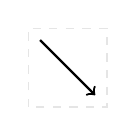
\begin{tikzpicture}
                \draw[white!90!black,dashed] (0,0) rectangle (1,1);
                \draw[thick,->] (0.15,0.85) -- (0.85,0.15);
            \end{tikzpicture}
        }
        \wrongchoice{
            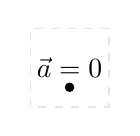
\begin{tikzpicture}
                \draw[white!90!black,dashed] (0,0) rectangle (1,1);
                \draw[fill] (0.5,0.25) circle (1.5pt)
                    node[anchor=south] {$\vec{a}=0$};
            \end{tikzpicture}
        }
        %\wrongchoice{There is no acceleration}
    \end{choices}
    \end{multicols}
\end{question}
}

\element{aapt}{ %% Bowl-D1
\begin{question}{bowl-2015-q08}
    A negatively charged balloon remains at rest when placed on a vertical wall.
    Which one of the following terms is most closely associated with the
        electrical phenomenon allowing the balloon to remain on the wall?
    \begin{multicols}{2}
    \begin{choices}
        \wrongchoice{Radiation}
        \wrongchoice{Grounding}
        \wrongchoice{Reduction}
        \wrongchoice{Current}
      \correctchoice{Polarization}
    \end{choices}
    \end{multicols}
\end{question}
}

\element{aapt}{ %% Bowl-A1
\begin{question}{bowl-2015-q09}
    Two cars are moving to the right on a horizontal track,
        each with constant acceleration.
    At an instant of time, the information about the cars is shown:
    \begin{description}
        \item[Car \#1:] position = \SI{125.0}{\meter};
            velocity = \SI{13.0}{\meter\per\second};
            constant acceleration = \SI{1.5}{\meter\per\second\squared}
        \item[Car \#2:] position = \SI{80.0}{\meter};
            velocity = \SI{9.30}{\meter\per\second};
            constant acceleration = \SI{5.5}{\meter\per\second\squared}
    \end{description}
    During the next \SI{1.0}{\second} of motion,
        which one of the following choices best represents
        what happens to the distance between the cars?
    \begin{choices}
        \wrongchoice{It decreases during the entire \SI{1.0}{\second} of motion.}
        \wrongchoice{It increases during the entire \SI{1.0}{\second} of motion.}
      \correctchoice{It initially increases and then decreases resulting in a greater distance between the cars after \SI{1.0}{\second}.}
        \wrongchoice{It initially increases and then decreases resulting in a smaller distance between the cars after \SI{1.0}{\second}.}
        \wrongchoice{It initially increases and then decreases resulting in the same distance between the cars after \SI{1.0}{\second}.}
    \end{choices}
\end{question}
}

\element{aapt}{ %% Bowl-D2
\begin{question}{bowl-2015-q10}
    For the circuit shown, the three light bulbs have identical resistance $R$,
        the battery is ideal, and all wires have no resistance.
    \begin{center}
    \ctikzset{bipoles/length=0.75cm}
    \begin{circuitikz}[scale=1.33]
        %% Parallel Circuit
        \draw (0,0) to [battery,l=$\xi$] (2,0)
                    to (2,1) to [R,l_=$\#3$] (0,1);
        \draw (2,1) to (2,2)
                    to [R,l_=$\#1$] (1,2)
                    to [R,l_=$\#2$] (0,2)
                    to (0,0);
        \draw (0,0.5) to (-0.5,0.5)
                    to [cspst,l=$S$] (-0.5,1.5)
                    to (0,1.5);
    \end{circuitikz}
    \end{center}
    Which one of the following choices correctly identifies the light bulbs
        that either become dimmer or go out completely when the switch,
        $S$, in the circuit is closed?
    \begin{choices}
        \wrongchoice{All 3 bulbs}
        \wrongchoice{Bulbs $\#1$ and $\#2$ only}
        \wrongchoice{Bulb $\#3$ only}
        \wrongchoice{Bulb $\#1$ only}
      \correctchoice{None of the bulbs}
    \end{choices}
\end{question}
}


%% PhysicsBowl 2015 Division 01 and 02
%%----------------------------------------
\element{aapt}{ %% Bowl-M1
\begin{question}{bowl-2015-q11}
    Two length measurements are made and recorded as
        $L_1=\SI{84.55}{\centi\meter}$ and $L_2=\SI{33.55}{\centi\meter}$.
    Two other length measurements are made and recorded as
        $L_3=\SI{1.750}{\centi\meter}$ and $L_4=\SI{1.250}{\centi\meter}$.
    These measurements are used to compute the quantity
        $\left( L_1 + L_2\right)-\left(L_3 + L_4\right)$ using the rules of significant figures.
    Which one of the following choices best represents the correct result to this calculation?
    \begin{multicols}{2}
    \begin{choices}
        \wrongchoice{\SI{115.100}{\centi\meter}}
      \correctchoice{\SI{115.10}{\centi\meter}}
        \wrongchoice{\SI{115.1}{\centi\meter}}
        \wrongchoice{\SI{115}{\centi\meter}}
        \wrongchoice{\SI{120}{\centi\meter}}
    \end{choices}
    \end{multicols}
\end{question}
}

\element{aapt}{ %% Bowl-A5
\begin{question}{bowl-2015-q12}
    A box of mass \SI{12.0}{\kilo\gram} is being pushed
        to the right across a horizontal surface.
    When the box has \SI{12.0}{\joule} of kinetic energy,
        a \SI{12.0}{\newton} net force acts on it.
    Which one of the following choices best represents the
        magnitude of the linear momentum of the box at this instant?
    \begin{multicols}{2}
    \begin{choices}
        \wrongchoice{\SI{6.00}{\kilo\gram\meter\per\second}}
        \wrongchoice{\SI{8.50}{\kilo\gram\meter\per\second}}
        \wrongchoice{\SI{12.0}{\kilo\gram\meter\per\second}}
      \correctchoice{\SI{17.0}{\kilo\gram\meter\per\second}}
        \wrongchoice{\SI{24.0}{\kilo\gram\meter\per\second}}
    \end{choices}
    \end{multicols}
\end{question}
}

\element{aapt}{ %% Bowl-A3
\begin{question}{bowl-2015-q13}
    An object is being pushed at constant speed on an inclined plane.
    The free body diagram of the object is shown with the gravitational force represented by $W$,
        the friction force by $f$,
        the applied external push parallel to the incline by $F$,
        and the normal force with the surface by $n$.
    %[Vectors are not drawn to scale.] ??
    \begin{center}
    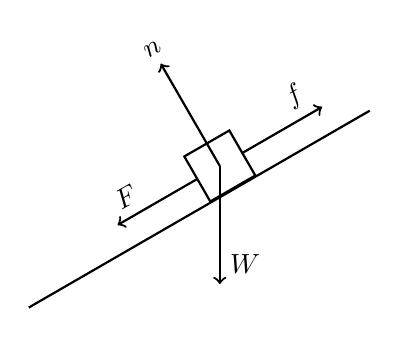
\begin{tikzpicture}
        %% Ramp
        \draw[thick] (0,0) -- (30:5cm);
        %% Box
        \node[thick,draw,rectangle,minimum size=0.66cm,rotate=30,anchor=south]
            (B) at (30:3cm) {};
        %% Arrows
        \draw[thick,->] (B) -- ++ (210:1.5cm)
            node[anchor=south west,rotate=30] {$F$};
        \draw[thick,->] (B) -- ++ (30:1.5cm)
            node[anchor=south east,rotate=30] {$f$};
        \draw[thick,->] (B.center) -- ++ (270:1.5cm)
            node[anchor=south west] {$W$};
        \draw[thick,->] (B.center) -- ++ (120:1.5cm)
            node[anchor=south,rotate=30] {$n$};
    \end{tikzpicture}
    \end{center}
    Which one of the following choices represents correct relationships between the forces?
    \begin{multicols}{2}
    \begin{choices}
        \wrongchoice{$n>W$ and $F<f$}
        \wrongchoice{$n<W$ and $F=f$}
      \correctchoice{$n<W$ and $F<f$}
        \wrongchoice{$n=W$ and $F>f$}
        \wrongchoice{$n=W$ and $F=f$}
    \end{choices}
    \end{multicols}
\end{question}
}

\element{aapt}{ %% Bowl-A2
\begin{question}{bowl-2015-q14}
    A particle has a position, $x$, as a function of time, $t$,
        given as $x(t) = -15 -25t + 10 t^2$, where all quantities are in base SI units.
    Which one of the following choices represents
        the magnitude of the particle's acceleration?
    \begin{multicols}{3}
    \begin{choices}
        \wrongchoice{\SI{5}{\meter\per\second\squared}}
        \wrongchoice{\SI{10}{\meter\per\second\squared}}
        \wrongchoice{\SI{15}{\meter\per\second\squared}}
      \correctchoice{\SI{20}{\meter\per\second\squared}}
        \wrongchoice{\SI{40}{\meter\per\second\squared}}
    \end{choices}
    \end{multicols}
\end{question}
}

\element{aapt}{ %% Bowl-A3
\begin{question}{bowl-2015-q15}
    A skydiver falls downward through the air with constant speed.
    Which one of the following choices correctly describes the
        Newton's Third Law pair force to the air resistance acting on the skydiver during the fall?
    \begin{choices}
        \wrongchoice{There is no Third Law pair force for this kind of situation.}
        \wrongchoice{The gravitational force acting on the skydiver by the Earth.}
        \wrongchoice{The force that molecules in the air exert on neighboring molecules in the air.}
        \wrongchoice{The force exerted on molecules in the air by the ground.}
      \correctchoice{The force exerted on molecules in the air by the skydiver.}
    \end{choices}
\end{question}
}

\element{aapt}{
\begin{question}{bowl-2015-q16}
    ``Particles of matter also have associated wavelengths and can behave as waves.''
    To which scientist is this concept attributed?
    \begin{multicols}{2}
    \begin{choices}
      \correctchoice{de Broglie}
        \wrongchoice{Pauli}
        \wrongchoice{Fermi}
        \wrongchoice{Heisenberg}
        \wrongchoice{Rydberg}
    \end{choices}
    \end{multicols}
\end{question}
}

\element{aapt}{ %% Bowl-A1
\begin{question}{bowl-2015-q17}
    An object starts at the origin and its velocity along a line vs. time is graphed.
    \begin{center}
    \begin{tikzpicture}
        \begin{axis}[
            axis y line=left,
            axis x line=middle,
            axis line style={->},
            xlabel={time},
            x unit=\si{\second},
            xtick={0,2,4,6,8,10},
            minor x tick num=1,
            ylabel={velocity},
            y unit=\si{\meter\per\second},
            ytick={-5,0,5},
            minor y tick num=4,
            grid=major,
            xmin=0,xmax=10.2,
            ymin=-5.5,ymax=5.5,
            width=0.95\columnwidth,
            height=0.50\columnwidth,
        ]
        \addplot[line width=1pt,mark=\empty] plot coordinates { (0,0) (3,4) (5,4) (9,-4) (10,-4) };
        \end{axis}
    \end{tikzpicture}
    \end{center}
    Which one of the following choices best gives the proper interval(s) of time for which the object is moving away from the origin?
    \begin{choices}
        \wrongchoice{Only for times $\SI{0}{\second}<t<\SI{3}{\second}$}
        \wrongchoice{Only for times $\SI{0}{\second}<t<\SI{5}{\second}$}
        \wrongchoice{Only for times $\SI{3}{\second}<t<\SI{5}{\second}$}
      \correctchoice{Only for times $\SI{0}{\second}<t<\SI{7}{\second}$}
        \wrongchoice{For times $\SI{0}{\second}<t<\SI{3}{\second}$ and $\SI{5}{\second}<t<\SI{9}{\second}$}
    \end{choices}
\end{question}
}

\element{aapt}{ %% Bowl-B4
\begin{question}{bowl-2015-q18}
    A \SI{680}{\hertz} tuning fork is placed over a tube open at both ends that is filled with air.
    As a result, a standing wave in the 3\textsuperscript{rd} harmonic is produced.
    The speed of sound in air is \SI{340}{\meter\per\second}.
    What is the length of the tube?
    \begin{multicols}{3}
    \begin{choices}
        \wrongchoice{\SI{0.38}{\meter}}
        \wrongchoice{\SI{0.67}{\meter}}
      \correctchoice{\SI{0.75}{\meter}}
        \wrongchoice{\SI{1.33}{\meter}}
        \wrongchoice{\SI{1.50}{\meter}}
    \end{choices}
    \end{multicols}
\end{question}
}

\element{aapt}{ %% Bowl-C3
\begin{question}{bowl-2015-q19}
    Ten moles of helium gas are enclosed in a container at a pressure of
        \SI{1.00}{atm} and at a temperature of \SI{400}{\kelvin}.
    Which one of the following choices best represents the density of this gas sample?
    \begin{multicols}{2}
    \begin{choices}
        \wrongchoice{\SI{0.012}{\kilo\gram\per\meter\cubed}}
      \correctchoice{\SI{0.12}{\kilo\gram\per\meter\cubed}}
        \wrongchoice{\SI{1.2}{\kilo\gram\per\meter\cubed}}
        \wrongchoice{\SI{120}{\kilo\gram\per\meter\cubed}}
        \wrongchoice{\SI{1.2e4}{\kilo\gram\per\meter\cubed}}
    \end{choices}
    \end{multicols}
\end{question}
}

\element{aapt}{ %% Bowl-??
\begin{question}{bowl-2015-q20}
    Which one of the following choices best represents the
        work for which the 2014 Nobel Prize in Physics was awarded?
    \begin{choices}
        \wrongchoice{Landing the Rosetta Philae Lander on the surface of Comet 67P/Churyumov-Gerasimenko}
        \wrongchoice{The detection of dark matter}
      \correctchoice{The invention of the blue LED}
        \wrongchoice{The creation of a tractor beam using sound}
        \wrongchoice{The detection of neutrinos from the Sun which agreed with theory}
    \end{choices}
\end{question}
}

\element{aapt}{ %% Bowl-A2
\begin{question}{bowl-2015-q21}
    An object is launched from the ground at an angle of \ang{60}
        above the horizontal with a speed of \SI{20.0}{\second}.
    What is the magnitude of the average velocity of the object
        from just after launch until it reaches its highest vertical position during flight?
    \begin{multicols}{2}
    \begin{choices}
        \wrongchoice{\SI{13.7}{\meter\per\second}}
      \correctchoice{\SI{13.2}{\meter\per\second}}
        \wrongchoice{\SI{10.0}{\meter\per\second}}
        \wrongchoice{\SI{9.3}{\meter\per\second}}
        \wrongchoice{\SI{8.7}{\meter\per\second}}
    \end{choices}
    \end{multicols}
\end{question}
}

\element{aapt}{ %% Bowl-A7
\begin{question}{bowl-2015-q22}
    Satellite 1 makes a circular orbit around the Earth with a radius $r_1=R$.
    Satellite 2 makes a circular orbit around the Earth with a radius $r_2=2R$.
    We let $v$ represent the speed of a satellite and $a$
        represent the magnitude of a satellite's acceleration.
    Which one of the following choices gives the correct relation
        between the speeds and accelerations of the satellites?
    \begin{choices}
      \correctchoice{$v_2=\dfrac{1}{\sqrt{2}}v_1$; $a_2=\dfrac{1}{4}a_1$}
        \wrongchoice{$v_2=\dfrac{1}{2}v_1$; $a_2=\dfrac{1}{4}a_1$}
        \wrongchoice{$v_2=\dfrac{1}{\sqrt{2}}v_1$; $a_2=\dfrac{1}{2}a_1$}
        \wrongchoice{$v_2=\dfrac{1}{2}v_1$; $a_2=\dfrac{1}{2}a_1$}
        \wrongchoice{$v_2=v_1$; $a_2=\dfrac{1}{2}a_1$}
    \end{choices}
\end{question}
}

\element{aapt}{ %% Bowl-A2
\begin{question}{bowl-2015-q23}
    A car moves with constant speed around a horseshoe-shaped
        path as shown with the arrows in the figure.
    \begin{center}
    \begin{tikzpicture}
    \begin{scope}[very thick,decoration={markings,mark=at position 0.5 with {\arrow{latex}}}]
        %% Inner bottom to inner upper
        \draw[postaction={decorate}] (2,-1.25) arc(270:450:0.125) -- (0,-1);
        \draw[postaction={decorate}] (0,-1) arc (270:90:1cm);
        \draw[postaction={decorate}] (0,+1) -- (2,1); %arc(270:450:0.125);
        %% outer upper to  outer bottom
        \draw[postaction={decorate}] (2,1) arc(270:450:0.125) -- (0,1.25) arc(90:180:1.25);
        \draw[postaction={decorate}] (-1.25,0) arc(180:270:1.25cm) -- (2,-1.25);
        %% X and W Labels
        \draw[fill] (1,-1.25) circle (2pt) node[anchor=north] {$W$};
        \draw[fill] (-1.25,0) circle (2pt) node[anchor=east] {$X$};
    \end{scope}
    \end{tikzpicture}
    \end{center}
    Which one of the following choices best describes the direction
        of the average acceleration of the car in traveling from $W$ to $X$?
    \begin{multicols}{3}
    \begin{choices}
        \AMCboxDimensions{down=-0.33cm}
        \correctchoice{
            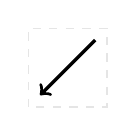
\begin{tikzpicture}
                \draw[white!90!black,dashed] (0,0) rectangle (1,1);
                \draw[very thick,->] (0.85,0.85) -- (0.15,0.15);
            \end{tikzpicture}
        }
        \wrongchoice{
            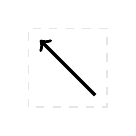
\begin{tikzpicture}
                \draw[white!90!black,dashed] (0,0) rectangle (1,1);
                \draw[very thick,->] (0.85,0.15) -- (0.15,0.85);
            \end{tikzpicture}
        }
        \wrongchoice{
            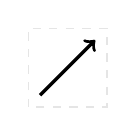
\begin{tikzpicture}
                \draw[white!90!black,dashed] (0,0) rectangle (1,1);
                \draw[very thick,->] (0.15,0.15) -- (0.85,0.85);
            \end{tikzpicture}
        }
        \wrongchoice{
            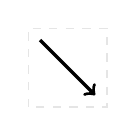
\begin{tikzpicture}
                \draw[white!90!black,dashed] (0,0) rectangle (1,1);
                \draw[very thick,->] (0.15,0.85) -- (0.85,0.15);
            \end{tikzpicture}
        }
        \wrongchoice{
            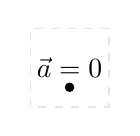
\begin{tikzpicture}
                \draw[white!90!black,dashed] (0,0) rectangle (1,1);
                \draw[fill] (0.5,0.25) circle (1.5pt) node[anchor=south] {$\vec{a}=0$};
            \end{tikzpicture}
        }
        %\wrongchoice{There is no average acceleration}
    \end{choices}
    \end{multicols}
\end{question}
}

\element{aapt}{ %% Bowl-A3
\begin{question}{bowl-2015-q24}
    A mass on a frictionless incline has a gravitational force,
        a normal force from the incline,
        and a force applied by a person that all are equal in magnitude.
    \begin{center}
    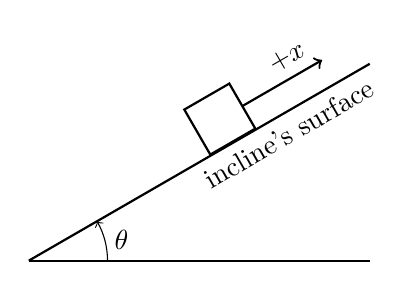
\begin{tikzpicture}
        %% Ramp
        \draw[thick] (0,0) -- (30:5cm)
            node[pos=1.00,anchor=north east,rotate=30] {incline's surface};
        \draw[thick] (0,0) -- (0:4.33cm);
        %% Angle
        \draw[->] (1.0,0) arc (0:30:1.0cm)
            node[pos=0.5,anchor=west] {$\theta$};
        %% Box
        \node[thick,draw,rectangle,minimum size=0.66cm,rotate=30,anchor=south]
            (B) at (30:3cm) {};
        %% Arrows
        \draw[thick,->] (B) -- ++ (30:1.5cm)
            node[pos=1.00,anchor=south east,rotate=30] {$+x$};
    \end{tikzpicture}
    \end{center}
    The mass remains at rest and the incline makes an angle $\theta$
        counterclockwise from the horizontal.
    Which one of the following choices best describes the
        orientation of the applied force by the person?
    The $+x$-axis is directed upward, parallel to the
        incline's surface as shown in the figure.
    \begin{choices}
        \wrongchoice{The applied force is oriented directly along the $+x$ axis.}
        \wrongchoice{The applied force is oriented at an angle $\theta$ clockwise from the $+x$ axis.}
      \correctchoice{The applied force is oriented at an angle $\ang{90}-\theta$ clockwise from the $+x$ axis.}
        \wrongchoice{The applied force is oriented at an angle $\ang{90}-\theta$ counterclockwise from the $+x$ axis.}
        \wrongchoice{This is a completely impossible situation that never can be realized physically.}
    \end{choices}
\end{question}
}

\element{aapt}{ %% Bowl-C3
\begin{question}{bowl-2015-q25}
    A gas undergoes the unusual process $M\rightarrow{}N$ in the pressure vs. volume graph shown.
    \begin{center}
    \begin{tikzpicture}
        \begin{axis}[
            axis y line=left,
            axis x line=bottom,
            axis line style={->},
            xlabel={volume},
            xtick=\empty,
            ylabel={pressure},
            ytick=\empty,
            grid=major,
            xmin=0,xmax=10,
            ymin=0,ymax=10,
            width=0.8\columnwidth,
            height=0.5\columnwidth,
        ]
        %% line
        \addplot[line width=1pt,smooth,tension=0.7,mark=\empty] plot coordinates {(6,8) (5,1) (3,3) (2,2) };
        %% arrows
        \draw[very thick,-latex] (axis cs:5.70,4.5) -- ++(260:0.5);
        \draw[very thick,-latex] (axis cs:3,3) -- ++(180:0.5);
        %% labels
        \fill (axis cs:2,2) circle (1.5pt) node[anchor=north] {$N$};
        \fill (axis cs:6,8) circle (1.5pt) node[anchor=south] {$M$};
        \end{axis}
    \end{tikzpicture}
    \end{center}
    Which one of the following choices properly represents the signs of the internal energy change of the gas, $\Delta U$,
        the total energy transferred as heat to the gas, $Q$,
        and the total work done on the gas by the surroundings, $W$, for this process?
    \begin{center}
    \begin{tabu}{cX[c]X[c]X[c]}
        \toprule
        \makebox[1.5em][c]{\textnumero}
            & $\Delta U$ & $Q$ & $W$ \\
        \bottomrule
    \end{tabu}
    \end{center}
    \begin{choices}
        \wrongchoice{\begin{tabu}{X[c]X[c]X[c]} Positive & Negative & Positive \\ \end{tabu}}
        \wrongchoice{\begin{tabu}{X[c]X[c]X[c]} Negative & Positive & Negative \\ \end{tabu}}
        \wrongchoice{\begin{tabu}{X[c]X[c]X[c]} Negative & Negative & Negative \\ \end{tabu}}
        \wrongchoice{\begin{tabu}{X[c]X[c]X[c]} Positive & Positive & Negative \\ \end{tabu}}
      \correctchoice{\begin{tabu}{X[c]X[c]X[c]} Negative & Negative & Positive \\ \end{tabu}}
    \end{choices}
\end{question}
}

\element{aapt}{ %% Bowl-A8
\begin{question}{bowl-2015-q26}
    The position of a mass connected to a spring obeys $x(t) = A\cos\left(\omega t\right)$.
    What is the average speed of the mass for one full oscillation
        in terms of the mass's maximum speed during oscillation, $v_{max}$?
    \begin{multicols}{2}
    \begin{choices}
      \correctchoice{$\dfrac{2}{\pi} v_{max}$}
        \wrongchoice{$\dfrac{1}{\sqrt{2}} v_{max}$}
        \wrongchoice{$\dfrac{1}{2} v_{max}$}
        \wrongchoice{$\dfrac{\sqrt{2}}{\pi} v_{max}$}
        \wrongchoice{$\dfrac{1}{2\pi\sqrt{2}} v_{max}$}
    \end{choices}
    \end{multicols}
\end{question}
}

\newcommand{\BowlTwentyFifteenQTwentySeven}{
\begin{tikzpicture}
    \begin{axis}[
        axis y line=left,
        axis x line=bottom,
        axis line style={->},
        xlabel={time},
        x unit=\si{\milli\second},
        xtick={0,1,2,3},
        ylabel={force},
        y unit=\si{\kilo\newton},
        ytick={0,5,10},
        grid=major,
        xmin=0,xmax=3,
        ymin=0,ymax=10,
        width=0.95\columnwidth,
        height=0.50\columnwidth,
    ]
    \addplot[line width=1pt,mark=\empty] plot coordinates {(0,0) (1,10) (3,0) };
    \end{axis}
\end{tikzpicture}
}

\element{aapt}{ %% Bowl-A5
\begin{question}{bowl-2015-q27}
    %Questions 27 – 28 deal with the following information:
    On a frictionless horizontal surface,
        two bodies make a head-on collision and stick together.
    Body 1 has a mass of \SI{3.50}{\kilo\gram} and initially moves
        to the right with speed \SI{7.0}{\meter\per\second}.
    Body 2 initially is at rest.
    A graph of the force exerted onto Body 2 from Body 1 during the collision is shown.
    \begin{center}
        \BowlTwentyFifteenQTwentySeven
    \end{center}
    What is the mass of Body 2?
    \begin{multicols}{3}
    \begin{choices}
        \wrongchoice{\SI{2.81}{\kilo\gram}}
        \wrongchoice{\SI{3.50}{\kilo\gram}}
        \wrongchoice{\SI{4.59}{\kilo\gram}}
      \correctchoice{\SI{5.53}{\kilo\gram}}
        \wrongchoice{\SI{7.50}{\kilo\gram}}
    \end{choices}
    \end{multicols}
\end{question}
}

\element{aapt}{ %% Bowl-A5
\begin{question}{bowl-2015-q28}
    %Questions 27 – 28 deal with the following information:
    On a frictionless horizontal surface,
        two bodies make a head-on collision and stick together.
    Body 1 has a mass of \SI{3.50}{\kilo\gram} and initially moves
        to the right with speed \SI{7.0}{\meter\per\second}.
    Body 2 initially is at rest.
    A graph of the force exerted onto Body 2 from Body 1 during the collision is shown.
    \begin{center}
        \BowlTwentyFifteenQTwentySeven
    \end{center}
    How much kinetic energy was transformed to other kinds of energy from the collision?
    \begin{multicols}{3}
    \begin{choices}
        \wrongchoice{\SI{67.1}{\joule}}
      \correctchoice{\SI{52.6}{\joule}}
        \wrongchoice{\SI{42.9}{\joule}}
        \wrongchoice{\SI{38.2}{\joule}}
        \wrongchoice{\SI{30.0}{\joule}}
    \end{choices}
    \end{multicols}
\end{question}
}

\element{aapt}{ %% Bowl-D4
\begin{question}{bowl-2015-q29}
    An electron moves at constant non-zero velocity directly between two long straight wires.
    The conventional current in each wire has the same magnitude,
        but the currents are in opposite directions as shown in the figure.
    \begin{center}
    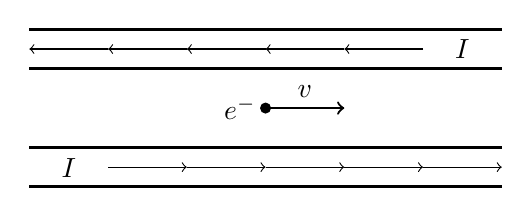
\begin{tikzpicture}
        %% NOTE: rotated 90 degrees
        %% electron
        \fill (0,0) circle (2pt) node[anchor=east] {$e^{-}$};
        \draw[thick,->] (0,0) -- (1,0) node[pos=0.5,anchor=south] {$v$};
        %% upper wire
        \draw[very thick] (-3,1) -- (3,1);
        \draw[very thick] (-3,0.5) -- (3,0.5);
        \node[anchor=south] at (+2.5,0.5) {$I$};
        \foreach \x in {-2,-1,...,2} {
            \draw[->] (\x,+0.75) -- ++(180:1);
        }
        %% lower wire
        \draw[very thick] (-3,-1) -- (3,-1);
        \draw[very thick] (-3,-0.5) -- (3,-0.5);
        \node[anchor=south] at (-2.5,-1.0) {$I$};
        \foreach \x in {-2,-1,...,2} {
            \draw[->] (\x,-0.75) -- ++(0:1);
        }
    \end{tikzpicture}
    \end{center}
    Ignoring gravity, which choice best reflects the direction of the magnetic field
        and the direction of the electric field that exist at the location of the electron?
    Any electric field in the region originates from an unseen external source.
    \begin{center}
    \begin{tabu}{cX[c]X[2c]}
        \toprule
        \makebox[1.5em][c]{\textnumero}
            & Electric Field & Magnetic Field \\
        \bottomrule
    \end{tabu}
    \end{center}
    \begin{choices}
        \wrongchoice{\begin{tabu}{X[c]X[2c]} No Field & No Field \\ \end{tabu}}
        \wrongchoice{\begin{tabu}{X[c]X[2c]} To the left & Into the plane of the page \\ \end{tabu}}
        \wrongchoice{\begin{tabu}{X[c]X[2c]} To the right & Into the plane of the page \\ \end{tabu}}
        \wrongchoice{\begin{tabu}{X[c]X[2c]} To the left & Out of the plane of the page \\ \end{tabu}}
      \correctchoice{\begin{tabu}{X[c]X[2c]} To the right & Out of the plane of the page \\ \end{tabu}}
    \end{choices}
\end{question}
}

\element{aapt}{ %% Bowl-??-F1
\begin{question}{bowl-2015-q30}
    A spring scale reads \SI{2.50}{\newton} when a small solid mass hangs from it in air.
    The spring scale reads \SI{1.58}{\newton} when the mass
        at the end of the spring is completely submerged in a container of water.
    Which one of the following choices best represents the density of the solid mass?
    \begin{multicols}{2}
    \begin{choices}
        \wrongchoice{\SI{3.68e3}{\kilo\gram\per\meter\cubed}}
      \correctchoice{\SI{2.72e3}{\kilo\gram\per\meter\cubed}}
        \wrongchoice{\SI{1.58e3}{\kilo\gram\per\meter\cubed}}
        \wrongchoice{\SI{9.20e2}{\kilo\gram\per\meter\cubed}}
        \wrongchoice{\SI{1.58e2}{\kilo\gram\per\meter\cubed}}
    \end{choices}
    \end{multicols}
\end{question}
}

\element{aapt}{ %% Bowl-??-C2
\begin{question}{bowl-2015-q31}
    Approximately how many hydrogen atoms are there in the liquid water of Earth's oceans?
    \begin{multicols}{3}
    \begin{choices}
        \wrongchoice{\num{e62}}
        \wrongchoice{\num{e57}}
        \wrongchoice{\num{e52}}
      \correctchoice{\num{e47}}
        \wrongchoice{\num{e42}}
    \end{choices}
    \end{multicols}
\end{question}
}

\element{aapt}{ %% Bowl-A1
\begin{question}{bowl-2015-q32}
    An object moving along a line completes a \SI{20.0}{\second}
        trip with an average speed of \SI{10.0}{\meter\per\second} in two stages.
    During stage 1, the object moves with a constant velocity of
        \SI{6.0}{\meter\per\second} to the right for \SI{12.0}{\second}.
    What constant magnitude acceleration directed to the left
        must the object have during the \SI{8.0}{\second} of stage 2?
    \begin{multicols}{2}
    \begin{choices}
        \wrongchoice{\SI{2.5}{\meter\per\second\squared}}
        \wrongchoice{\SI{2.7}{\meter\per\second\squared}}
        \wrongchoice{\SI{4.0}{\meter\per\second\squared}}
      \correctchoice{\SI{5.3}{\meter\per\second\squared}}
        \wrongchoice{\SI{6.3}{\meter\per\second\squared}}
    \end{choices}
    \end{multicols}
\end{question}
}

\element{aapt}{ %% Bowl-B4
\begin{question}{bowl-2015-q33}
    Two spherical speakers separated by \SI{30.0}{\meter} each emit a
        constant frequency signal of \SI{57.0}{\hertz} in phase with each other.
    The speed of sound in air is \SI{342}{\meter\per\second}.
    \begin{center}
    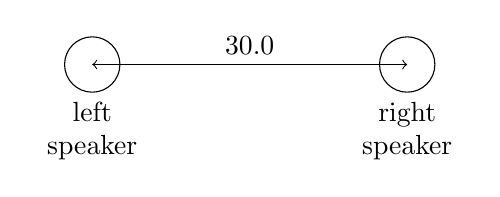
\begin{tikzpicture}
        \draw (-2,0) circle (1em);
        \node[anchor=north,text width=4em,text centered] at (-2,-1em) {left speaker};
        \node[anchor=north,text width=4em,text centered] at (+2,-1em) {right speaker};
        \draw (+2,0) circle (1em);
        \draw[<->] (-2,0) -- (+2,0) node[pos=0.5,anchor=south] {\SI{30.0}{\meter}};
    \end{tikzpicture}
    \end{center}
    How many locations of complete destructive interference of the
        incoming signals are there on the line between the speakers?
    \begin{multicols}{3}
    \begin{choices}
        \wrongchoice{\num{12}}
        \wrongchoice{\num{11}}
      \correctchoice{\num{10}}
        \wrongchoice{\num{9}}
        \wrongchoice{\num{6}}
    \end{choices}
    \end{multicols}
\end{question}
}

\element{aapt}{ %% Bowl-B2
\begin{question}{bowl-2015-q34}
    An upward-pointing object is placed \SI{15.0}{\centi\meter} to the left of a lens system.
    The first lens is convex with focal length \SI{10.0}{\centi\meter}.
    The second lens is convex with focal length \SI{10}{\centi\meter} and its location from the first lens is varied from \SI{10}{\centi\meter} away to \SI{110}{\centi\meter} away.
    \emph{Please Note:} The drawings are not drawn to scale.
    \begin{center}
    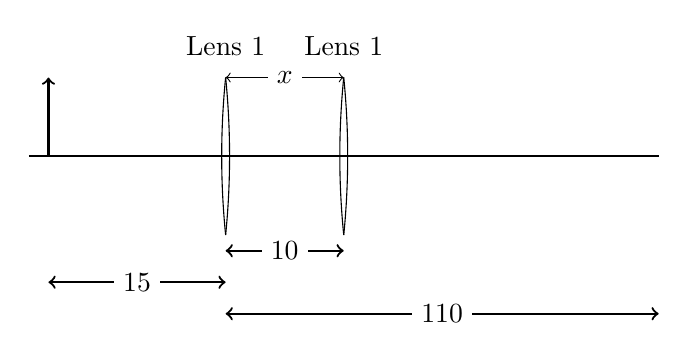
\begin{tikzpicture}
        %% optical axis
        \draw[thick] (-3,0) -- (5,0);
        %% object
        \draw[thick,->] (-2.75,0) -- (-2.75,1);
        %% lens 1
        \draw (-0.5,1) arc (5.74:-5.74:10);
        \draw (-0.5,1) arc (174.26:185.74:10);
        \node[anchor=south,yshift=1ex] at (-0.5,1) {Lens 1};
        %% lens 2
        \draw (+1,1) arc (5.74:-5.74:10);
        \draw (+1,1) arc (174.26:185.74:10);
        \node[anchor=south,yshift=1ex] at (+1,1) {Lens 1};
        %% distance x
        \draw[<->] (-0.5,1) -- (+1,1) node[pos=0.5,anchor=center,fill=white] {$x$};
        \draw[thick,<->] (-0.5,-1.2) -- (+1,-1.2) node[pos=0.5,anchor=center,fill=white] {\SI{10}{\centi\meter}};
        \draw[thick,<->] (-0.5,-1.6) -- (-2.75,-1.6) node[pos=0.5,anchor=center,fill=white] {\SI{15}{\centi\meter}};
        \draw[thick,<->] (-0.5,-2) -- (+5,-2) node[pos=0.5,anchor=center,fill=white] {\SI{110}{\centi\meter}};
    \end{tikzpicture}
    \end{center}
    Which one of the following choices best represents the description of the final image formed as the second lens is moved from $x=\SI{10}{\centi\meter}$ to $x=\SI{110}{\centi\meter}$ from the first lens?
    \begin{center}
    \begin{tabu}{cX[c]X[c]X[c]}
        \toprule
        \makebox[1.5em][c]{\textnumero}
            & $x=\SI{10}{\centi\meter}$
            & $\longrightarrow~~~\longrightarrow~~~\longrightarrow$
            & $x=\SI{110}{\centi\meter}$ \\
        \bottomrule
    \end{tabu}
    \end{center}
    \begin{choices}
      \correctchoice{\begin{tabu}{X[c]X[c]X[c]} Real and pointing downward & Virtual and pointing downward & Real and pointing upward \\ \midrule \end{tabu}}
        \wrongchoice{\begin{tabu}{X[c]X[c]X[c]} Virtual and pointing downward & Virtual and pointing upward & Real and pointing upward \\ \midrule \end{tabu}}
        \wrongchoice{\begin{tabu}{X[c]X[c]X[c]} Virtual and pointing upward & Virtual and pointing downward & Real and pointing upward \\ \midrule \end{tabu}}
        \wrongchoice{\begin{tabu}{X[c]X[c]X[c]} Real and pointing upward & Virtual and pointing downward & Real and pointing upward \\ \midrule \end{tabu}}
        \wrongchoice{\begin{tabu}{X[2c]X[c]} Virtual and pointing downward & Real and pointing upward \\ \midrule \end{tabu}}
    \end{choices}
\end{question}
}

\element{aapt}{ %% Bowl-A6
\begin{question}{bowl-2015-q35}
    Two uniform disks, $X$ and $Y$, have equal masses, $M$,
        but different radii such that $r_X < r_Y$.
    Both disks initially are at rest.
    A force $F$ is applied tangent to each disk at its right edge for the same amount of time.
    \begin{center}
    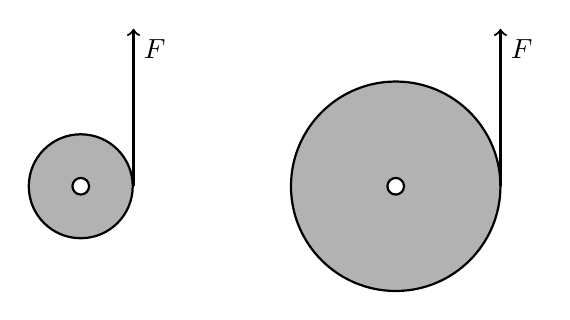
\begin{tikzpicture}
        \draw[thick,fill=white!70!black] (-2,0) circle (0.66);
        \draw[thick,fill=white] (-2,0) circle (3pt);
        \draw[thick,->] (-1.33,0) -- ++ (90:2cm)
            node[pos=1.0,anchor=north west] {$F$};
        \draw[thick,fill=white!70!black] (+2,0) circle (1.33);
        \draw[thick,fill=white] (+2,0) circle (3pt);
        \draw[thick,->] (3.33,0) -- ++ (90:2cm)
            node[pos=1.0,anchor=north west] {$F$};
    \end{tikzpicture}
    \end{center}
    As a result, each disk rotates counterclockwise in the plane
        of the page about a fixed frictionless axis through its center.
    Which one of the following choices correctly compares the
        magnitudes of angular momentum $L$ about the center axis and
        total kinetic energy $K$ of disk $X$ and disk $Y$?
    \begin{choices}
        \wrongchoice{$L_x<L_y$; $K_X<K_Y$}
        \wrongchoice{$L_x<L_y$; $K_X>K_Y$}
        \wrongchoice{$L_x=L_y$; $K_X=K_Y$}
        \wrongchoice{$L_x=L_y$; $K_X<K_Y$}
      \correctchoice{$L_x<L_y$; $K_X=K_Y$}
    \end{choices}
\end{question}
}

\element{aapt}{ %% Bowl-A2
\begin{question}{bowl-2015-q36}
    Rain falls vertically at \SI{12.0}{\meter\per\second} with respect to a stationary observer.
    A car is moving at an angle of \ang{40} below the horizontal with respect to the observer.
    A passenger sitting in the car notes that the rain makes an angle of \ang{29.0} with the vertical.
    What is the car's speed with respect to the observer?
    \begin{multicols}{2}
    \begin{choices}
        \wrongchoice{\SI{2.29}{\meter\per\second}}
      \correctchoice{\SI{5.39}{\meter\per\second}}
        \wrongchoice{\SI{9.03}{\meter\per\second}}
        \wrongchoice{\SI{11.8}{\meter\per\second}}
        \wrongchoice{\SI{16.2}{\meter\per\second}}
    \end{choices}
    \end{multicols}
\end{question}
}

\element{aapt}{ %% Bowl-D5
\begin{question}{bowl-2015-q37}
    Which one of the following choices represents the base SI units of inductance?
    \begin{multicols}{3}
    \begin{choices}
      \correctchoice{$\dfrac{\si{\kilo\gram\meter\squared}}{\si{\ampere\squared\second\squared}}$}
        \wrongchoice{$\dfrac{\si{\kilo\gram\meter\squared}}{\si{\ampere\second}}$}
        \wrongchoice{$\dfrac{\si{\kilo\gram\meter}}{\si{\ampere\squared\second\squared}}$}
        \wrongchoice{$\dfrac{\si{\kilo\gram\meter\squared}}{\si{\ampere\squared\second\cubed}}$}
        \wrongchoice{$\dfrac{\si{\kilo\gram\meter}}{\si{\ampere\squared\second\cubed}}$}
    \end{choices}
    \end{multicols}
\end{question}
}

\element{aapt}{ %% Bowl-B2
\begin{question}{bowl-2015-q38}
    A thin film of alcohol ($n_{alcohol}=1.35$) lies on a flat glass surface ($n_{glass}=1.60$).
    When light of wavelength \SI{540}{\nano\meter} is incident normal to the alcohol surface from air,
        the light is strongly reflected, but when light of wavelength \SI{432}{\nano\meter}
        is incident normal to the surface from air, the reflected light is minimized.
    \begin{center}
    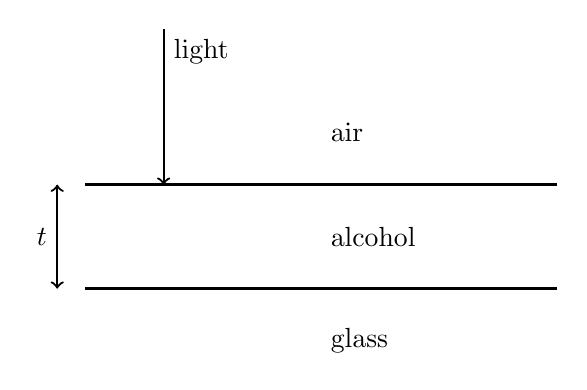
\begin{tikzpicture}[yscale=0.66]
        %% Boundaries
        \draw[very thick] (0,2) -- (6,2);
        \draw[very thick] (0,0) -- (6,0);
        %% Lebels
        \node[anchor=west] at (3,3) {air};
        \node[anchor=west] at (3,1) {alcohol};
        \node[anchor=west] at (3,-1) {glass};
        %% Thickness
        \draw[thick,<->] (-1em,0) -- (-1em,2) node[pos=0.5,anchor=east] {$t$};
        %% Incoming Ray
        \draw[thick,->] (1,5) -- (1,2) node[pos=0.0,anchor=north west] {light};
    \end{tikzpicture}
    \end{center}
    Which one of the following choices could represent the thickness, $t$, of the alcohol film?
    \begin{multicols}{3}
    \begin{choices}
        \wrongchoice{\SI{216}{\nano\meter}}
        \wrongchoice{\SI{320}{\nano\meter}}
        \wrongchoice{\SI{324}{\nano\meter}}
      \correctchoice{\SI{400}{\nano\meter}}
        \wrongchoice{\SI{486}{\nano\meter}}
    \end{choices}
    \end{multicols}
\end{question}
}

\element{aapt}{ %% Bowl-D2
\begin{question}{bowl-2015-q39}
    For the circuit shown, the four light bulbs have identical resistance,
        the battery is ideal and all wires have no resistance.
    \begin{center}
    \ctikzset{bipoles/length=0.75cm}
    \begin{circuitikz}[scale=1.5]
        \draw (0,0) to [battery,l=$\xi$] (0,2)
                    to (2,2) to [R] (2,1)
                    to [R] (2,0) to (0,0);
        \draw (2,2) to (4,2) to (4,1) to [R] (4,0) to (2,0);
        \draw (2,1) to [cspst,l=$S$] (3,1) to [R] (4,1);
        \draw[fill] (0,0) circle (1pt) node[anchor=east] {$P$};
        \draw[fill] (4,1) circle (1pt) node[anchor=west] {$X$};
        \draw[fill] (2,1) circle (1pt) node[anchor=east] {$W$};
    \end{circuitikz}
    \end{center}
    After the switch, $S$, in the circuit is closed,
        which one of the following choices correctly describes what happens to the magnitude of the current at the point labeled $P$ and to the magnitude of the potential difference from $W$ to $X$?
    \begin{center}
    \begin{tabu}{cX[c]X[c]}
        \toprule
        \makebox[1.5em][c]{\textnumero}
            & Current at $P$ & $\Delta V_{XW}$ \\
        \bottomrule
    \end{tabu}
    \end{center}
    \begin{choices}
        \wrongchoice{\begin{tabu}{X[c]X[c]} No Change & Increases \\ \end{tabu}}
        \wrongchoice{\begin{tabu}{X[c]X[c]} Decreases & Increases \\ \end{tabu}}
        \wrongchoice{\begin{tabu}{X[c]X[c]} Increases & Increases \\ \end{tabu}}
        \wrongchoice{\begin{tabu}{X[c]X[c]} Decreases & Decreases \\ \end{tabu}}
      \correctchoice{\begin{tabu}{X[c]X[c]} Increases & Decreases \\ \end{tabu}}
    \end{choices}
\end{question}
}

\element{aapt}{ %% Bowl-A3
\begin{question}{bowl-2015-q40}
    A \SI{2.0}{\kilo\gram} mass is connected to the end of string and moves about the string's fixed end in a conical motion with a constant speed of \SI{4.0}{\meter\per\second}.
    The string has a length of \SI{2.50}{\meter} and forms an angle of $\theta$ with the vertical.
    \begin{center}
    \begin{tikzpicture}
        %% Ceiling
        \node[anchor=south,fill,pattern=north east lines,minimum width=4cm, minimum height=0.05cm] at (0,0) {};
        \draw (-2,0) -- (2,0);
        %% Pendulum Bob
        \node[fill,draw,circle,minimum size=1em] (A) at (225:3cm) {};
        \draw (0,0) -- (A);
        %% Circular path
        \draw[dashed] (0,-2.21) circle (2.21cm and 0.5cm);
        %% Angle
        \draw[dashed] (0,0) -- (0,-2.21);
        \draw[<->] (225:1cm) arc (225:270:1cm) node[pos=0.5,anchor=north] {$\theta$};
    \end{tikzpicture}
    \end{center}
    What is the tension in the string?
    \begin{multicols}{2}
    \begin{choices}
        \wrongchoice{\SI{20.0}{\newton}}
        \wrongchoice{\SI{23.7}{\newton}}
      \correctchoice{\SI{27.4}{\newton}}
        \wrongchoice{\SI{29.8}{\newton}}
        \wrongchoice{\SI{32.5}{\newton}}
    \end{choices}
    \end{multicols}
\end{question}
}


%% PhysicsBowl 2015 Division 02 only
%%----------------------------------------
\newcommand{\BowlTwentyFifteenQFortyOne}{
\begin{tikzpicture}
    \begin{axis}[
        axis y line=left,
        axis x line=bottom,
        axis line style={->},
        xlabel={time},
        xtick={0,5,10},
        xticklabels={$0$,$T$,$2T$},
        ylabel={position},
        ytick=\empty,
        grid=major,
        xmin=0,xmax=11,
        ymin=0,ymax=20,
        width=0.95\columnwidth,
        height=0.50\columnwidth,
        very thin,
        legend style={
            at={(0.90,0.1)},
            anchor=south,
        },
        colormap={mymap}{rgb=(0,0,0); rgb=(0,0,0)}
    ]
    \addplot[dashed,line width=1pt,domain=0:10]{4+(8*x/5)};
    \addplot[line width=1pt,black,draw=black,color=black,patch,patch type=quadratic spline] coordinates {
        (0,4) (5,12) (2,2.0) (5,12) (10,20) (7,18) };
    %\legend{Truck,Car}; node??
    \end{axis}
\end{tikzpicture}
}

\element{aapt}{ %% Bowl-A1
\begin{question}{bowl-2015-q41}
    %Questions 41--42 deal with the following information:
    A car (solid line) and a truck (dashed line) are moving on a horizontal track.
    The position vs. time graph for the two vehicles is shown.
    \begin{center}
        \BowlTwentyFifteenQFortyOne
    \end{center}
    For the entire time shown in the graph,
        which one of the following choices correctly describes the relationship
        between the average speed of the truck to that of the car?
    \begin{choices}
      \correctchoice{The truck's average speed is less than the average speed of the car.}
        \wrongchoice{The truck's average speed is the same as the average speed of the car.}
        \wrongchoice{The truck's average speed is greater than the average speed of the car.}
        \wrongchoice{The truck's average speed is positive while the car's average speed is negative but of the same magnitude.}
        \wrongchoice{A relationship cannot be determined without more information.}
    \end{choices}
\end{question}
}

\element{aapt}{ %% Bowl-A1
\begin{question}{bowl-2015-q42}
    %Questions 41--42 deal with the following information:
    A car (solid line) and a truck (dashed line) are moving on a horizontal track.
    The position vs. time graph for the two vehicles is shown.
    \begin{center}
        \BowlTwentyFifteenQFortyOne
    \end{center}
    Which one of the following choices best describes the instants of time, $t$,
        at which the car and truck travel with the same speed?
    \begin{choices}
        \wrongchoice{Only at times $t=0$, $t=T$ and $t=2T$.}
        \wrongchoice{At one instant during the interval $0 < t < T$ and at one instant during the interval $T < t < 2T$.}
      \correctchoice{At two instants during the interval $0 < t < T$ and at one instant during the interval $T < t < 2T$.}
        \wrongchoice{At one instant during the interval $0 < t < T$ and at two instants during the interval $T < t < 2T$.}
        \wrongchoice{At two instants during the interval $0 < t < T$ and at two instants during the interval $T < t < 2T$.}
    \end{choices}
\end{question}
}

\element{aapt}{ %% Bowl-A5
\begin{question}{bowl-2015-q43}
    An object of mass \SI{4.0}{\kilo\gram} has a total kinetic energy of
        \SI{100.0}{\joule} and an $x$-component of
        linear momentum equal to \SI{24.0}{\kilo\gram\meter\per\second}.
    The object is moving in the $x$-$y$ plane.
    What is the $y$-component of the object's linear momentum?
    \begin{multicols}{2}
    \begin{choices}
        \wrongchoice{\SI{8.00}{\kilo\gram\meter\per\second}}
      \correctchoice{\SI{15.0}{\kilo\gram\meter\per\second}}
        \wrongchoice{\SI{26.0}{\kilo\gram\meter\per\second}}
        \wrongchoice{\SI{32.0}{\kilo\gram\meter\per\second}}
        \wrongchoice{\SI{97.0}{\kilo\gram\meter\per\second}}
    \end{choices}
    \end{multicols}
\end{question}
}

\element{aapt}{ %% Bowl-C2
\begin{question}{bowl-2015-q44}
    Which one of the following choices is most associated with the following statement:
        ``When the pressure of a gas is held constant,
        the volume of the gas is directly proportional to the temperature.''?
    \begin{multicols}{2}
    \begin{choices}
        \wrongchoice{Newton's Law}
        \wrongchoice{Boyle's Law}
        \wrongchoice{Avogadro's Law}
        \wrongchoice{Graham's Law}
      \correctchoice{Charles's Law}
    \end{choices}
    \end{multicols}
\end{question}
}

\element{aapt}{ %% Bowl-D1
\begin{question}{bowl-2015-q45}
    A \SI{6.00}{\micro\farad} parallel-plate capacitor is disconnected
        from a \SI{12}{\volt} battery after being fully charged.
    A person now carefully inserts a dielectric material of constant
        $\kappa=2$ so that it fills one-half of the space between the plates as shown.
    \begin{center}
    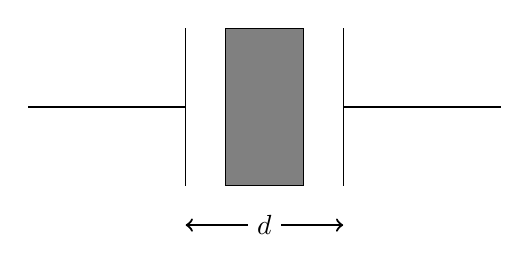
\begin{tikzpicture}
        %% Left Capacitor Plate
        \draw (-1,0) -- (-1,2);
        \draw (-3,1) -- (-1,1);
        %% Right Capacitor Plate
        \draw (+1,0) -- (+1,2);
        \draw (+3,1) -- (+1,1);
        %% Thickness
        \draw[thick,<->] (-1,-0.5) -- (+1,-0.5)
            node[pos=0.5,anchor=center,fill=white] {$d$};
        %% Dielectric
        \draw[fill=white!50!black] (-0.5,0) rectangle (+0.5,2);
    \end{tikzpicture}
    \end{center}
    How much work was done by the person while inserting the dielectric?
    \begin{multicols}{3}
    \begin{choices}
        \wrongchoice{\SI{-81}{\micro\joule}}
      \correctchoice{\SI{-108}{\micro\joule}}
        \wrongchoice{\SI{-144}{\micro\joule}}
        \wrongchoice{\SI{-216}{\micro\joule}}
        \wrongchoice{\SI{-288}{\micro\joule}}
    \end{choices}
    \end{multicols}
\end{question}
}

\element{aapt}{ %% Bowl-A6
\begin{question}{bowl-2015-q46}
    A uniform rod of mass $M$ and length $L$ is fixed to rotate about a
        frictionless pivot located $\frac{L}{3}$ from one end.
    The rod is released from rest incrementally away from being perfectly vertical,
        resulting in the rod rotating clockwise about the pivot.
    \begin{center}
    \begin{tikzpicture}
        \draw[thick] (0,-1) -- (0,2);
        \draw[fill] (0,0) circle (2pt) node[label distance=1em,pin=45:pivot] {};
        \node[anchor=west] at (0,-0.5) {$\dfrac{L}{3}$};
        \draw[thick,dashed,->] (0,-1) arc (270:240:1cm);
        \draw[thick,dashed,->] (0,2) arc (90:60:2cm);
    \end{tikzpicture}
    \end{center}
    When the rod is horizontal,
        what is the magnitude of the tangential acceleration of its center of mass?
    \begin{multicols}{3}
    \begin{choices}
        \wrongchoice{$\dfrac{1}{6} g$}
        \wrongchoice{$\dfrac{1}{2} g$}
        \wrongchoice{$\dfrac{4}{3} g$}
        \wrongchoice{$\dfrac{2}{3} g$}
      \correctchoice{$\dfrac{1}{4} g$}
    \end{choices}
    \end{multicols}
\end{question}
}

\element{aapt}{ %% Bowl-C3
\begin{question}{bowl-2015-q47}
    One mole of a diatomic ideal gas undergoes a reversible adiabatic process.
    The pressure and volume initially are given as $P=\SI{2.0}{atm}$ and $V=\SI{30}{\liter}$.
    If the volume is halved during the adiabatic process,
        how much work was done on the gas sample by the surroundings?
    \begin{multicols}{3}
    \begin{choices}
        \wrongchoice{\SI{6790}{\joule}}
        \wrongchoice{\SI{5530}{\joule}}
      \correctchoice{\SI{4850}{\joule}}
        \wrongchoice{\SI{4200}{\joule}}
        \wrongchoice{\SI{3040}{\joule}}
    \end{choices}
    \end{multicols}
\end{question}
}

\element{aapt}{ %% Bowl-D1
\begin{question}{bowl-2015-q48}
    Two concentric charged conducting shells are in free space.
    The outer shell has inner radius $2a$ and outer radius $3a$.
    The inner shell has radius $a$.
    \begin{center}
    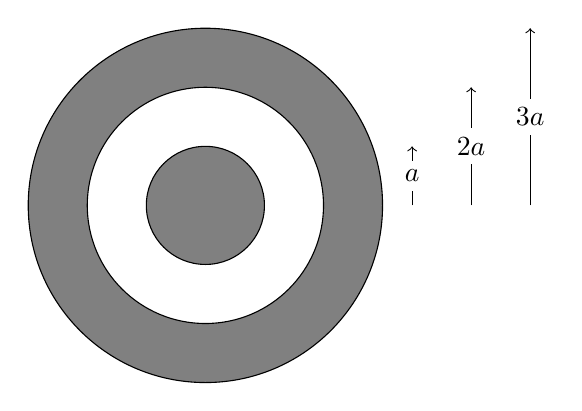
\begin{tikzpicture}[scale=0.75]
        \draw[fill=white!50!black] (0,0) circle (3.0cm);
        \draw[fill=white]          (0,0) circle (2.0cm);
        \draw[fill=white!50!black] (0,0) circle (1.0cm);
        \draw[->] (3.5,0) -- ++ (90:1cm) node[fill=white,anchor=center,pos=0.5] {$a$};
        \draw[->] (4.5,0) -- ++ (90:2cm) node[fill=white,anchor=center,pos=0.5] {$2a$};
        \draw[->] (5.5,0) -- ++ (90:3cm) node[fill=white,anchor=center,pos=0.5] {$3a$};
    \end{tikzpicture}
    \end{center}
    It is known that the electric potential at $r=3a$ is $V_{3a}= \frac{kQ}{3a}$.
    If the electric potential $V_{a}$ at $r=a$ is \SI{0}{\volt},
        what is the charge on the inner spherical shell, $Q_{in}$?
    \begin{multicols}{2}
    \begin{choices}
        \wrongchoice{$Q_{in}= -\frac{3}{2} Q$}
      \correctchoice{$Q_{in}= -\frac{2}{3} Q$}
        \wrongchoice{$Q_{in}= -\frac{1}{3} Q$}
        \wrongchoice{$Q_{in}= - 2Q$}
        \wrongchoice{$Q_{in}= -\frac{1}{2} Q$}
    \end{choices}
    \end{multicols}
\end{question}
}

\element{aapt}{ %% Bowl-E3
\begin{question}{bowl-2015-q49}
    The kinetic energy associated with an electron is twice its rest energy.
    At what speed is the electron traveling?
    \begin{multicols}{2}
    \begin{choices}
      \correctchoice{\SI{2.83e8}{\meter\per\second}}
        \wrongchoice{\SI{2.67e8}{\meter\per\second}}
        \wrongchoice{\SI{2.60e8}{\meter\per\second}}
        \wrongchoice{\SI{2.25e8}{\meter\per\second}}
        \wrongchoice{\SI{2.12e8}{\meter\per\second}}
    \end{choices}
    \end{multicols}
\end{question}
}

\element{aapt}{ %% Bowl-D5
\begin{question}{bowl-2015-q50}
    A magnetic field directed into the plane of the page is decreasing in time.
    A constant emf $\xi$ is produced for the square loop enclosing the field in the figure.
    \begin{center}
    \ctikzset{bipoles/length=0.75cm}
    \begin{circuitikz}
        %% circuit
        \draw (0,0) to [voltmeter] (4,4) to (4,0);
        \draw (0,0) to (0,4) to [R,l=$R$] (2,4) to [R,l=$R$] (4,4) to (4,0) to [R,l=$R$] (0,0);
        %% B field into page
        \foreach \x in {0.5,1.0,...,3.5}
            \foreach \y in {0.5,1.0,...,3.5}
                \foreach \i in {45,135,225,315} {
                    \pgfmathifthenelse{\x==\y}{}{"\noexpand\draw[thick] (\x,\y) -- ++(\i:0.1);"}\pgfmathresult
                }
    \end{circuitikz}
    \end{center}
    The square loop has three identical light bulbs of resistance $R$
        in it and an ideal voltmeter connected to the corners through the center of the loop.
    What is the magnitude of the voltmeter's reading?
    \begin{multicols}{3}
    \begin{choices}
        \wrongchoice{$0\xi$}
        \wrongchoice{$\dfrac{1}{2}\xi$}
        \wrongchoice{$\dfrac{1}{3}\xi$}
      \correctchoice{$\dfrac{1}{6}\xi$}
        \wrongchoice{$\dfrac{2}{3}\xi$}
    \end{choices}
    \end{multicols}
\end{question}
}


%% PhysicsBowl 2014 Division 01 only
%%----------------------------------------
\element{aapt1}{ %% Bowl-B1
\begin{question}{bowl-2014-q01}
    An FM radio station sends a signal with a frequency
        of \SI{99.99e6}{\hertz}.
    Which one of the following choices best represents
        this frequency expressed using metric prefixes?
    \begin{multicols}{2}
    \begin{choices}
        \wrongchoice{\SI{99.99}{\kilo\hertz}.}
      \correctchoice{\SI{99.99}{\mega\hertz}.}
        \wrongchoice{\SI{99.99}{\giga\hertz}.}
        \wrongchoice{\SI{99.99}{\tera\hertz}.}
        \wrongchoice{\SI{99.99}{\nano\hertz}.}
    \end{choices}
    \end{multicols}
\end{question}
}

\element{aapt}{ %% Bowl-M1
\begin{question}{bowl-2014-q02}
    In the laboratory, a student makes the following six measurements for the length of an object: \SI{5.05}{\centi\meter},
        \SI{5.06}{\centi\meter}, \SI{5.07}{\centi\meter}, \SI{5.07}{\centi\meter}, and \SI{5.09}{\centi\meter}.
    Using the rules of significant digits, which one of the following choices correctly represents how she should express the average length of the object?
    \begin{multicols}{3}
    \begin{choices}
        \wrongchoice{\SI{5}{\centi\meter}.}
        \wrongchoice{\SI{5.06}{\centi\meter}.}
        %\wrongchoice{\SI[parse-numbers=false]{5.0\bar{66}}{\centi\meter}.}
        \wrongchoice{\SI{5.066}{\centi\meter}.}
      \correctchoice{\SI{5.07}{\centi\meter}.}
        \wrongchoice{\SI{5.1}{\centi\meter}.}
    \end{choices}
    \end{multicols}
\end{question}
}

\element{aapt}{ %% Bowl-A2
\begin{question}{bowl-2014-q03}
    An object is dropped into free fall.
    Through how many meters does the object fall during the first \SI{3.00}{\second} of flight?
    \begin{multicols}{3}
    \begin{choices}
        \wrongchoice{\SI{10.0}{\meter}.}
        \wrongchoice{\SI{15.0}{\meter}.}
        \wrongchoice{\SI{30.0}{\meter}.}
      \correctchoice{\SI{45.0}{\meter}.}
        \wrongchoice{\SI{90.0}{\meter}.}
    \end{choices}
    \end{multicols}
\end{question}
}

\element{aapt}{ %% Bowl-A3
\begin{question}{bowl-2014-q04}
    Three equal masses are suspended from a classroom ceiling by a series of strings as shown in the figure.
    \begin{center}
    \begin{tikzpicture}[yscale=0.75]
        %% Ceiling
        \draw (-2,0) -- (2,0);
        \node[anchor=south,pattern=north east lines,minimum width=4cm,minimum height=0.05cm] at (0,0) {};
        %% Masses
        \node[draw,rectangle,anchor=center,minimum size=0.75cm] (A) at (0,-2) {$M$};
        \node[draw,rectangle,anchor=center,minimum size=0.75cm] (B) at (0,-4) {$M$};
        \node[draw,rectangle,anchor=center,minimum size=0.75cm] (C) at (0,-6) {$M$};
        %% Strings
        \draw[thick] (0,0) -- (A.north) node[pos=0.5,anchor=west] {$A$};
        \draw[thick] (A.south) -- (B.north) node[pos=0.5,anchor=west] {$B$};
        \draw[thick] (B.south) -- (C.north) node[pos=0.5,anchor=west] {$C$};
    \end{tikzpicture}
    \end{center}
    Which string has the greatest tension?
    \begin{choices}
      \correctchoice{Only String $A$.}
        \wrongchoice{Only String $B$.}
        \wrongchoice{Only String $C$.}
        \wrongchoice{Strings $A$, $B$, and $C$ have the same non-zero tension.}
        \wrongchoice{Strings $A$, $B$, and $C$ all have no tension.}
    \end{choices}
\end{question}
}

\element{aapt}{ %% Bowl-A8
\begin{question}{bowl-2014-q05}
    A simple pendulum consists of a massive bob connected to the end of a very light string.
    Which one of the following changes should be made in order to increase the period of the pendulum?
    Ignore air resistance.
    \begin{choices}
        \wrongchoice{Increase the mass of the bob.}
        \wrongchoice{Decrease the mass of the bob.}
      \correctchoice{Increase the length of the string.}
        \wrongchoice{Decrease the length of the string.}
        \wrongchoice{Decrease the maximum angle of the pendulum's oscillation.}
    \end{choices}
\end{question}
}

\element{aapt}{ %% Bowl-??-E2
\begin{question}{bowl-2014-q06}
    MRI is a commonly used acronym for medical diagnostic technique.
    MRI stands for which of the the following choices?
    \begin{choices}
        \wrongchoice{Medical Radio Imaging.}
        \wrongchoice{Minimally Radioactive Intervention.}
        \wrongchoice{Multiaxis Radar Injection.}
        \wrongchoice{Magnetic Radioisotopic Injection.}
      \correctchoice{Magnetic Resonance Imaging.}
    \end{choices}
\end{question}
}

\element{aapt}{ %% Bowl-A1
\begin{question}{bowl-2014-q07}
    Starting from rest,
        a car uniformly accelerates to a speed of \SI{7.60}{\meter\per\second} in a time of \SI{3.00}{\second}.
    Through what distance does the cart move in this time?
    \begin{multicols}{3}
    \begin{choices}
        \wrongchoice{\SI{5.7}{\meter}}
        \wrongchoice{\SI{8.1}{\meter}}
      \correctchoice{\SI{11.4}{\meter}}
        \wrongchoice{\SI{16.1}{\meter}}
        \wrongchoice{\SI{22.8}{\meter}}
    \end{choices}
    \end{multicols}
\end{question}
}

\element{aapt}{ %% Bowl-A8
\begin{question}{bowl-2014-q08}
    A \SI{2.5}{\kilo\gram} mass connected to the end of an ideal spring oscillates in simple harmonic motion.
    The mass''s position is described as a function of time by $x(t) = 0.20 \cos\left(8.00 t + 0.50\right)$ where all quantities are in base SI units.
    Which of the following choices gives the numerical value of the oscillation's amplitude in base SI units?
    \begin{multicols}{3}
    \begin{choices}
        \wrongchoice{\num{8.00}}
        \wrongchoice{\num{4.00}}
        \wrongchoice{\num{1.60}}
        \wrongchoice{\num{0.50}}
      \correctchoice{\num{0.20}}
    \end{choices}
    \end{multicols}
\end{question}
}

\element{aapt}{ %% Bowl-A4
\begin{question}{bowl-2014-q09}
    Which one of the following quantities is not a scalar quantity?
    \begin{multicols}{3}
    \begin{choices}
      \correctchoice{Force}
        \wrongchoice{Energy}
        \wrongchoice{Mass}
        \wrongchoice{Speed}
        \wrongchoice{Pressure}
    \end{choices}
    \end{multicols}
\end{question}
}

\element{aapt}{ %% Bowl-D1
\begin{question}{bowl-2014-q10}
    Two charges, $-Q$ and $+Q$, are fixed in place on the $x$-axis,
        each a distance $a$ from the origin as shown.
    \begin{center}
    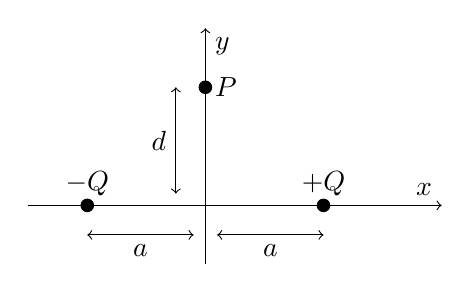
\begin{tikzpicture}[scale=1.5]
        %% Axes
        \draw[->] (-1.5,0) -- (2,0) node[pos=1.0,anchor=south east] {$x$};
        \draw[->] (0,-0.5) -- (0,1.5) node[pos=1.0,anchor=north west] {$y$};
        %% Location labels
        \draw[fill] (-1,0) circle (1.5pt) node[anchor=south] {$-Q$};
        \draw[fill] (+1,0) circle (1.5pt) node[anchor=south] {$+Q$};
        \draw[fill] (0,+1) circle (1.5pt) node[anchor=west] {$P$};
        %% Distance labels
        \draw[<->] (-1,-0.25) -- (-0.1,-0.25) node[pos=0.5,anchor=north] {$a$};
        \draw[<->] (+1,-0.25) -- (0.1,-0.25) node[pos=0.5,anchor=north] {$a$};
        \draw[<->] (-0.25,1) -- (-0.25,0.1) node[pos=0.5,anchor=east] {$d$};
    \end{tikzpicture}
    \end{center}
    At the point labeled $P$, a distance $d$ along the $y$-axis from the origin,
        what is the direction of the electric field from the given charges?
    \begin{choices}
        \wrongchoice{Up the plan of the page}
        \wrongchoice{Down the plane of the page}
        \wrongchoice{To the right}
      \correctchoice{To the left}
        \wrongchoice{There is no electric field}
    \end{choices}
\end{question}
}


%% PhysicsBowl 2014 Division 01 and 02
%%----------------------------------------
\element{aapt}{ %% Bowl-A4
\begin{question}{bowl-2014-q11}
    A crate gains \SI{36.0}{\joule} of kinetic energy while its speed is increased from \SI{2.00}{\meter\per\second} to \SI{4.00}{\meter\per\second}.
    Which one of the following choices best represents the mass of the crate?
    \begin{multicols}{3}
    \begin{choices}
        \wrongchoice{\SI{36.0}{\kilo\gram}}
        \wrongchoice{\SI{18.0}{\kilo\gram}}
      \correctchoice{\SI{6.0}{\kilo\gram}}
        \wrongchoice{\SI{3.0}{\kilo\gram}}
        \wrongchoice{\SI{1.5}{\kilo\gram}}
    \end{choices}
    \end{multicols}
\end{question}
}

\element{aapt}{ %% Bowl-A3
\begin{question}{bowl-2014-q12}
    A box of mass \SI{5.0}{\kilo\gram} is being pushed to the right across a horizontal surface while a constant frictional force of \SI{8.0}{\newton} acts on the box.
    At some instant of time,
        the box has a speed of \SI{4.0}{\meter\per\second} and an acceleration of \SI{3.0}{\meter\per\second\squared}.
    What is the magnitude of the net force acting on the box at this instant?
    \begin{multicols}{3}
    \begin{choices}
        \wrongchoice{\SI{7.0}{\newton}}
        \wrongchoice{\SI{12.0}{\newton}}
      \correctchoice{\SI{15.0}{\newton}}
        \wrongchoice{\SI{20.0}{\newton}}
        \wrongchoice{\SI{23.0}{\newton}}
    \end{choices}
    \end{multicols}
\end{question}
}

\element{aapt}{ %% Bowl-A4
\begin{question}{bowl-2014-q13}
    Which one of the following scientists is most associated with the following statement:
        ``For small displacements of an object from equilibrium, there is a restoring force that is proportional to the displacement''?
    \begin{multicols}{2}
    \begin{choices}
        \wrongchoice{Albert Einstein}
      \correctchoice{Robert Hooke}
        \wrongchoice{Christiaan Huygens}
        \wrongchoice{Johannes Kepler}
        \wrongchoice{Heinrich Lenz}
    \end{choices}
    \end{multicols}
\end{question}
}

\element{aapt}{ %% Bowl-A3
\begin{question}{bowl-2014-q14}
    A box rests on the floor of an elevator.
    The elevator is accelerating upward.
    Which one of the following choices best represents the Newton's Third Law pair force to the gravitational force acting on the box by the Earth?
    \begin{choices}
        \wrongchoice{There is no Newton's Third Law pair force in this scenario.}
        \wrongchoice{The entire normal force of contact from the floor on the box.}
        \wrongchoice{Only a portion of the normal force of contact from the floor on the box.}
        \wrongchoice{The force of the cables pulling upward on the elevator.}
      \correctchoice{The gravitational force acting on the Earth by the box.}
    \end{choices}
\end{question}
}

\element{aapt}{ %% Bowl-A5
\begin{question}{bowl-2014-q15}
    Two objects $A$ and $B$, move in space and then collide.
    \begin{description}
        \item[Before collision:] Object $A$, of mass \SI{5.0}{\kilo\gram},
            moves to the right with a speed of \SI{25.0}{\meter\per\second}.
            Object $B$ of mass \SI{10.0}{\kilo\gram}, moves to the left with a speed of \SI{20.0}{\meter\per\second}.
        \item[After collision:] Object $A$ moves to the left with a speed of \SI{25.0}{\meter\per\second}.
    \end{description}
    What is the velocity of object $B$ after the collision?
    \begin{multicols}{2}
    \begin{choices}
        \wrongchoice{\SI{30.0}{\meter\per\second} to the right}
        \wrongchoice{\SI{20.0}{\meter\per\second} to the right}
        \wrongchoice{\SI{20.0}{\meter\per\second} to the left}
      \correctchoice{\SI{5.0}{\meter\per\second} to the right}
        \wrongchoice{\SI{5.0}{\meter\per\second} to the left}
    \end{choices}
    \end{multicols}
\end{question}
}

\element{aapt}{ %% Bowl-A1
\begin{question}{bowl-2014-q16}
    A toy car initially moves to the right at \SI{60.0}{\centi\meter\per\second}.
    Five seconds later, the car is moving at \SI{40.0}{\centi\meter\per\second} to the left.
    The total displacement of the car during this time is \SI{10.0}{\centi\meter} to the left of where it started.
    Which one of the following choices best represents the magnitude of the average velocity of the car during the five second motion?
    \begin{multicols}{2}
    \begin{choices}
        \wrongchoice{\SI{50.0}{\centi\meter\per\second}}
        \wrongchoice{\SI{10.0}{\centi\meter\per\second}}
        \wrongchoice{\SI{4.0}{\centi\meter\per\second}}
      \correctchoice{\SI{2.0}{\centi\meter\per\second}}
        \wrongchoice{\SI{0.40}{\centi\meter\per\second}}
    \end{choices}
    \end{multicols}
\end{question}
}

\element{aapt}{ %% Bowl-A1
\begin{question}{bowl-2014-q17}
    A toy car initially moves to the right at \SI{60.0}{\centi\meter\per\second}.
    Five seconds later, the car is moving at \SI{40.0}{\centi\meter\per\second} to the left.
    The total displacement of the car during this time is \SI{10.0}{\centi\meter} to the left of where it started.
    Which one of the following choices best represents the magnitude of the average acceleration of the car during the five second motion?
    \begin{multicols}{2}
    \begin{choices}
      \correctchoice{\SI{20.0}{\centi\meter\per\second\squared}}
        \wrongchoice{\SI{4.0}{\centi\meter\per\second\squared}}
        \wrongchoice{\SI{2.0}{\centi\meter\per\second\squared}}
        \wrongchoice{\SI{0.80}{\centi\meter\per\second\squared}}
        \wrongchoice{\SI{0.40}{\centi\meter\per\second\squared}}
    \end{choices}
    \end{multicols}
\end{question}
}

\element{aapt}{ %% Bowl-M1
\begin{question}{bowl-2014-q18}
    A rectangular block of wood has a mass of \SI{17.8}{\gram} and dimensions of length: \SI{3.00}{\centi\meter},
        width: \SI{4.00}{\centi\meter}, and height: \SI{2.00}{\centi\meter}.
    Which one of the following choices correctly gives the average density of the block?
    \begin{multicols}{2}
    \begin{choices}
        \wrongchoice{\SI{7.42e5}{\kilo\gram\per\meter\cubed}}
      \correctchoice{\SI{7.42e2}{\kilo\gram\per\meter\cubed}}
        \wrongchoice{\SI{7.42}{\kilo\gram\per\meter\cubed}}
        \wrongchoice{\SI{7.42e-1}{\kilo\gram\per\meter\cubed}}
        \wrongchoice{\SI{7.42e-4}{\kilo\gram\per\meter\cubed}}
    \end{choices}
    \end{multicols}
\end{question}
}

\element{aapt}{ %% Bowl-??-E3
\begin{question}{bowl-2014-q19}
    In 2013, the Nobel Prize in physics was awarded
        ``for the theoretical discovery of a mechanism that contributes to our understanding of the origin of mass of subatomic particles,
          and which recently was confirmed through the discovery of the predicted fundamental particle,
          by the ATLAS and CMS experiment at CERN's Large Hadron Collider.''
    The winners were Fran\c{c}ois Englert and:
    \begin{multicols}{2}
    \begin{choices}
        \wrongchoice{Stephen Hawking}
        \wrongchoice{Edward Witten}
        \wrongchoice{Edwin Hubble}
        \wrongchoice{Brian Greene}
      \correctchoice{Peter Higgs}
    \end{choices}
    \end{multicols}
\end{question}
}

\element{aapt}{ %% Bowl-A3
\begin{question}{bowl-2014-q20}
    A uniform block of mass $m$ is placed on an inclined plane of angle $\theta$.
    \begin{center}
    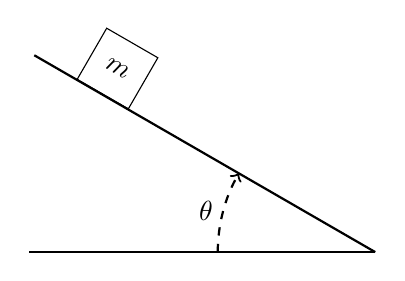
\begin{tikzpicture}
        %% Ramp
        \draw[thick] (0,0) -- ++ (150:5cm);
        \draw[thick] (0,0) -- ++ (180:4.4cm);
        %% Angle
        \draw[thick,->,dashed] (-2cm,0) arc (180:150:2cm) node[pos=0.5,anchor=east] {$\theta$};
        %% Box
        \node[draw,rotate=-30,minimum size=0.75cm,anchor=south] at (150:4cm) {$m$};
    \end{tikzpicture}
    \end{center}
    When released, the block does not move.
    It is determined that the normal force acting on the incline on the block has a magnitude of \SI{62}{\newton} while the force of static friction acting on the block has a magnitude of \SI{38}{\newton}.
    The coefficient of static friction between the block and inclined plane is $\mu_s = \num{0.92}$.
    Which one of the following choices best represents the mass, $m$, of the block?
    \begin{multicols}{3}
    \begin{choices}
        \wrongchoice{\SI{2.4}{\kilo\gram}}
        \wrongchoice{\SI{6.2}{\kilo\gram}}
      \correctchoice{\SI{7.3}{\kilo\gram}}
        \wrongchoice{\SI{8.4}{\kilo\gram}}
        \wrongchoice{\SI{10.0}{\kilo\gram}}
    \end{choices}
    \end{multicols}
\end{question}
}

\element{aapt}{ %% Bowl-B4
\begin{question}{bowl-2014-q21}
    A tuning fork placed over a \SI{57}{\centi\meter} column of air closed only at its bottom end produces a standing wave in the 3\textsuperscript{rd} harmonic.
    The speed of sound in air is \SI{342}{\meter\per\second}.
    What is the frequency of the tuning fork?
    \begin{multicols}{3}
    \begin{choices}
        \wrongchoice{\SI{150}{\hertz}}
        \wrongchoice{\SI{300}{\hertz}}
      \correctchoice{\SI{450}{\hertz}}
        \wrongchoice{\SI{600}{\hertz}}
        \wrongchoice{\SI{900}{\hertz}}
    \end{choices}
    \end{multicols}
\end{question}
}

\element{aapt}{ %% Bowl-D2
\begin{question}{bowl-2014-q22}
    For the circuit shown, all three light bulbs have the same resistance.
    \begin{center}
    \ctikzset{bipoles/length=0.75cm}
    \begin{circuitikz}[scale=1.33]
        \draw (0,0) to (0,2) to [battery,l=$\xi$] (2,2) to [R,l=\#1] (3,2) to (3,0) to (2,0) to [R,l_=\#3] (0,0);
        \draw (2,2) to [R,l=\#2] (2,0);
    \end{circuitikz}
    \end{center}
    The battery and wires have no resistance.
    What is the proper ranking of the bulbs' brightness?
    \begin{choices}
        \wrongchoice{Bulb 1 $=$ Bulb 2 $=$ Bulb 3}
        \wrongchoice{Bulb 3 $<$ Bulb 2 $=$ Bulb 1}
        \wrongchoice{Bulb 2 $<$ Bulb 1 $<$ Bulb 3}
      \correctchoice{Bulb 1 $=$ Bulb 2 $<$ Bulb 3}
        \wrongchoice{Bulb 1 $=$ Bulb 3 $<$ Bulb 2}
    \end{choices}
\end{question}
}

\element{aapt}{ %% Bowl-A6
\begin{question}{bowl-2014-q23}
    Two small identical coins (labeled $X$ and $Y$) are at rest on a horizontal disk rotating at a constant rate about an axis perpendicular to the plan of the disk and through its center.
    \begin{center}
    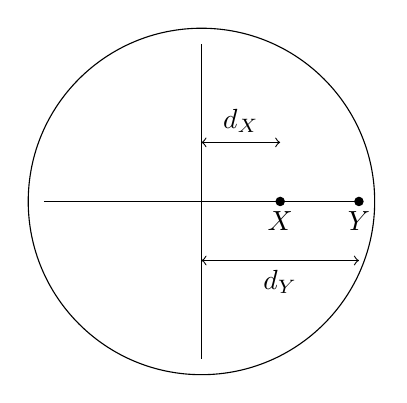
\begin{tikzpicture}
        \draw (0,0) circle (2.2cm);
        %% Axis
        \draw (0,-2) -- (0,+2);
        \draw (-2,0) -- (+2,0);
        %% Lables X and Y
        \draw[fill] (+1,0) circle (1.5pt) node[anchor=north] {$X$};
        \draw[fill] (+2,0) circle (1.5pt) node[anchor=north] {$Y$};
        %% Distances
        \draw[<->] (0,0.75) -- (1,0.75) node[pos=0.5,anchor=south] {$d_X$};
        \draw[<->] (0,-0.75) -- (2,-0.75) node[pos=0.5,anchor=north] {$d_Y$};
    \end{tikzpicture}
    \end{center}
    The distance of the coins from the center of disk is related by $d_X=\frac{1}{2} d_Y$.
    Which one of the following choices correctly identifies the relationship between $f_X$ and $f_Y$,
        the frictional force on coin $X$ and on coin $Y$, respectively?
    \begin{multicols}{2}
    \begin{choices}
        \wrongchoice{$f_X = \dfrac{1}{4} f_Y$}
      \correctchoice{$f_X = \dfrac{1}{2} f_Y$}
        \wrongchoice{$f_X = f_Y$}
        \wrongchoice{$f_X = 2 f_Y$}
        \wrongchoice{$f_X = 4 f_Y$}
    \end{choices}
    \end{multicols}
\end{question}
}

\element{aapt}{ %% Bowl-D4
\begin{question}{bowl-2014-q24}
    For the bar magnet shown in the figure,
        which choice best describes the direction of the magnetic field at the point $P$ located directly above the center of the magnet?
    \begin{center}
    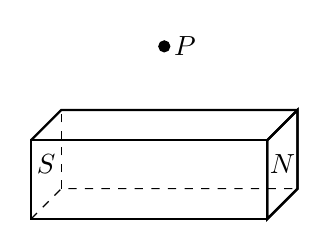
\begin{tikzpicture}
        %% Cube
        \draw[thick] (0,0,0) -- (3,0,0) -- (3,1,0) -- (0,1,0) -- cycle;
        \draw[thick] (3,0,0) -- (3,0,-1) -- (3,1,-1) -- (3,1,0) -- cycle;
        \draw[thick] (3,0,0) -- (3,0,-1) -- (3,1,-1) -- (3,1,0) -- cycle;
        \draw[thick] (0,1,0) -- (0,1,-1) -- (3,1,-1);
        \draw[dashed] (0,0,0) -- (0,0,-1) -- (3,0,-1);
        \draw[dashed] (0,0,-1) -- (0,1,-1);
        %% Labels
        %% NOTE: TODO: slant text
        \draw[fill] (1.5,2.0,-0.5) circle (2pt) node[anchor=west] {$P$};
        \node[anchor=center] at (3.0,0.5,-0.5) {$N$};
        \node[anchor=center] at (0.0,0.5,-0.5) {$S$};
    \end{tikzpicture}
    \end{center}
    \begin{choices}
        \wrongchoice{Up the plane of the page}
        \wrongchoice{To the right}
        \wrongchoice{Down the plane of the page}
      \correctchoice{To the left}
        \wrongchoice{Out of the plane of the page}
    \end{choices}
\end{question}
}

\element{aapt}{ %% Bowl-B2
\begin{question}{bowl-2014-q25}
    It is observed that a light ray changes direction when it enters a new material.
    Which one of the following choices is the term best associated with this phenomenon?
    \begin{multicols}{2}
    \begin{choices}
        \wrongchoice{Doppler Effect}
        \wrongchoice{Interference}
        \wrongchoice{Polarization}
        \wrongchoice{Diffraction}
      \correctchoice{Refraction}
    \end{choices}
    \end{multicols}
\end{question}
}

\element{aapt}{ %% Bowl-??-F1
\begin{question}{bowl-2014-q26}
    A solid cube of iron and a solid cube of aluminum have equal mass.
    The cubes are placed into the same large pool of water so that each is completely submerged and resting on the pool's bottom.
    Which object experiences the greater buoyant force from the water?
    \begin{choices}
        \wrongchoice{The iron cube}
      \correctchoice{The aluminum cube}
        \wrongchoice{The buoyant forces are equal}
        \wrongchoice{The mass of the cubes is needed to answer the question.}
        \wrongchoice{The answer depends on the whether the pool is filled with fresh water or salt water.}
    \end{choices}
\end{question}
}

\element{aapt}{ %% Bowl-A7
\begin{question}{bowl-2014-q27}
    Two spherical, non-rotating planets, $X$ and $Y$, have the same density $\rho$.
    Planet $X$ has twice the radius of planet $Y$.
    Let $g_X$ and $g_Y$ represent the acceleration due to gravity at the surfaces of Planet $X$ and planet $Y$, respectively.
    What is the ratio of $g_X:g_Y$?
    \begin{multicols}{3}
    \begin{choices}
      \correctchoice{$2:1$}
        \wrongchoice{$1:2$}
        \wrongchoice{$1:1$}
        \wrongchoice{$4:1$}
        \wrongchoice{$1:4$}
    \end{choices}
    \end{multicols}
\end{question}
}

\element{aapt4}{ %% Bowl-B4
\begin{question}{bowl-2014-q28}
    A waterproof speaker placed at the bottom of a swimming pool emits a sound wave that travels toward the surface of the water.
    In the water, the sound wave has a frequency $f_{water}$,
        wavelength $\lambda_{water}$, and wave speed $v_{water}$.
    When the sound wave enters the air it has frequency $f_{air}$,
        wavelength $\lambda_{water}$, and wave speed $v_{water}$.
    Which one of the following relationships correctly compares the frequencies,
        wavelengths, and wave speeds of the waves in the air and water?
    \begin{choices}
        \wrongchoice{$f_{water}=f_{air}$; $\lambda_{water}=\lambda{air}$; $v_{water}=v_{air}$}
      \correctchoice{$f_{water}=f_{air}$; $\lambda_{water}>\lambda{air}$; $v_{water}>v_{air}$}
        \wrongchoice{$f_{water}<f_{air}$; $\lambda_{water}>\lambda{air}$; $v_{water}=v_{air}$}
        \wrongchoice{$f_{water}<f_{air}$; $\lambda_{water}=\lambda{air}$; $v_{water}<v_{air}$}
        \wrongchoice{$f_{water}=f_{air}$; $\lambda_{water}<\lambda{air}$; $v_{water}>v_{air}$}
    \end{choices}
\end{question}
}

\element{aapt}{ %% Bowl-D4
\begin{question}{bowl-2014-q29}
    An electron with charge $-e$ and mass $m$ travels at a speed $v$
        in a plane perpendicular to the magnetic field of magnitude $B$.
    The electron follows a circular path of radius $R$.
    In a time $t$, the electron travels halfway around the circle.
    What is the amount of work done by the magnetic force on the
        electron in this time?
    \begin{multicols}{2}
    \begin{choices}
      \correctchoice{zero}
        \wrongchoice{$-\pi evBR$}
        \wrongchoice{$\pi evBR$}
        \wrongchoice{$-2\pi evBR$}
        \wrongchoice{$\dfrac{\pi mv}{eB}$}
    \end{choices}
    \end{multicols}
\end{question}
}

\element{aapt}{ %% Bowl-A7
\begin{question}{bowl-2014-q30}
    Considering only the Moon-Earth system (ignore any influence of the Sun),
        which one of the following best represents the magnitude of the Moon's acceleration about the Earth?
    \begin{multicols}{2}
    \begin{choices}
        \wrongchoice{\SI{3e-1}{\meter\per\second\squared}}
        \wrongchoice{\SI{3e-2}{\meter\per\second\squared}}
      \correctchoice{\SI{3e-3}{\meter\per\second\squared}}
        \wrongchoice{\SI{3e-4}{\meter\per\second\squared}}
        \wrongchoice{\SI{3e-5}{\meter\per\second\squared}}
    \end{choices}
    \end{multicols}
\end{question}
}

\element{aapt}{ %% Bowl-A4
\begin{question}{bowl-2014-q31}
    A toy crane exerts an upward force and delivers a useful power output of \SI{0.10}{\watt} to raise a block vertically at a constant speed.
    At what constant speed will this crane raise a \SI{0.20}{\kilo\gram} block?
    \begin{multicols}{3}
    \begin{choices}
        \wrongchoice{\SI{0.01}{\meter\per\second}}
        \wrongchoice{\SI{0.02}{\meter\per\second}}
      \correctchoice{\SI{0.05}{\meter\per\second}}
        \wrongchoice{\SI{0.20}{\meter\per\second}}
        \wrongchoice{\SI{0.50}{\meter\per\second}}
    \end{choices}
    \end{multicols}
\end{question}
}

\element{aapt}{ %% Bowl-A4
\begin{question}{bowl-2014-q32}
    Planck's constant is multiplied by the speed of light.
    The resulting value then is divided by three meters.
    This final value has the units of which one of the following quantities?
    \begin{multicols}{2}
    \begin{choices}
        \wrongchoice{Force}
        \wrongchoice{Linear Momentum}
        \wrongchoice{Speed}
        \wrongchoice{Frequency}
      \correctchoice{Energy}
    \end{choices}
    \end{multicols}
\end{question}
}

\element{aapt}{ %% Bowl-A1
\begin{question}{bowl-2014-q33}
    An object moves with constant acceleration starting with velocity $v_0=\SI{5.00}{\meter\per\second}$ and ending with a velocity of $v=-\SI{1.00}{\meter\per\second}$ in a time of \SI{3.00}{\second}.
    For this motion, what is the average speed associated with the object.
    \begin{multicols}{3}
    \begin{choices}
        \wrongchoice{\SI{2.00}{\meter\per\second}}
      \correctchoice{\SI{2.17}{\meter\per\second}}
        \wrongchoice{\SI{2.50}{\meter\per\second}}
        \wrongchoice{\SI{2.83}{\meter\per\second}}
        \wrongchoice{\SI{3.00}{\meter\per\second}}
    \end{choices}
    \end{multicols}
\end{question}
}

\element{aapt}{ %% Bowl-D5
\begin{question}{bowl-2014-q34}
    Two circular loops of resistive wire are placed next to each other as in the figure.
    \begin{center}
    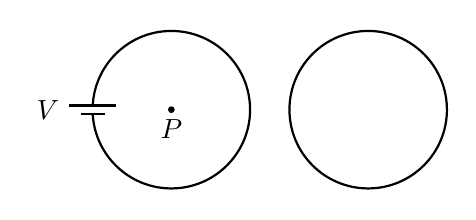
\begin{tikzpicture}
        %% Battery
        \node[anchor=east] at (180:1.30cm) {$V$};
        %% Left Circle
        \draw[thick] (177:1cm) -- ++ (0:0.30cm);
        \draw[thick] (177:1cm) -- ++ (180:0.30cm);
        \draw[thick] (-177:1cm) -- ++ (0:0.15cm);
        \draw[thick] (-177:1cm) -- ++ (180:0.15cm);
        \draw[thick] (-177:1cm) arc (-177:177:1cm);
        %% Right Circle
        \draw[thick] (2.5,0) circle (1cm);
        \draw[fill] (0,0) circle (1pt) node[anchor=north] {$P$};
    \end{tikzpicture}
    \end{center}
    The circular loop on the left is connected to a constant voltage source $V$.
    The resistance of this loop is increasing linearly with time.
    As the resistance is changing,
        what is the direction of the magnetic field at point $P$ (the center of the left-hand loop) and what is the orientation of the conventional current in the right-hand loop (as viewed in the figure from above)?
    \begin{center}
    \begin{tabu}{cX[5c]X[4c]}
        \toprule
        \makebox[1.5em][c]{\textnumero}
            & Magnetic Field Direction & Current Orientation \\
        \bottomrule
    \end{tabu}
    \end{center}
    \begin{choices}
      \correctchoice{\begin{tabu}{X[5c]X[4c]} Into the plane of the page & Counterclockwise \\ \end{tabu}}
        \wrongchoice{\begin{tabu}{X[5c]X[4c]} Into the plane of the page & Clockwise \\ \end{tabu}}
        \wrongchoice{\begin{tabu}{X[5c]X[4c]} Out of the plane of the page & Counterclockwise \\ \end{tabu}}
        \wrongchoice{\begin{tabu}{X[5c]X[4c]} Out of the plane of the page & Counterclockwise \\ \end{tabu}}
        \wrongchoice{\begin{tabu}{X[5c]X[4c]} There is no field & There is no current \\ \end{tabu}}
    \end{choices}
\end{question}
}

\element{aapt}{ %% Bowl-??
\begin{question}{bowl-2014-q35}
    There are several statements presented below that attempt to describe physical phenomena.
    Which one of the following statements is correct?
    \begin{choices}
        \wrongchoice{The coefficient of friction is a value always less than or equal to one, but greater than or equal to zero.}
        \wrongchoice{For horizontal surfaces, the normal force acting on an object always cancels the gravitational force.}
        \wrongchoice{An ideal gas's temperature must change if both work is done and energy is exchanged as heat with it.}
        \wrongchoice{Increasing the spacing between slits in the Young's double slit experiment results in an increase in the spacing between the dark regions on a distant viewing screen.}
      \correctchoice{In electrostatic equilibrium, an electric field is perpendicular to the surface of a charged conductor electrostatic equilibrium, an electric field is perpendicular to the surface of a charged conductor.}
    \end{choices}
\end{question}
}

\element{aapt}{ %% Bowl-B2
\begin{question}{bowl-2014-q36}
    A concave mirror with focal length $f$ is shown in the figure.
    \begin{center}
    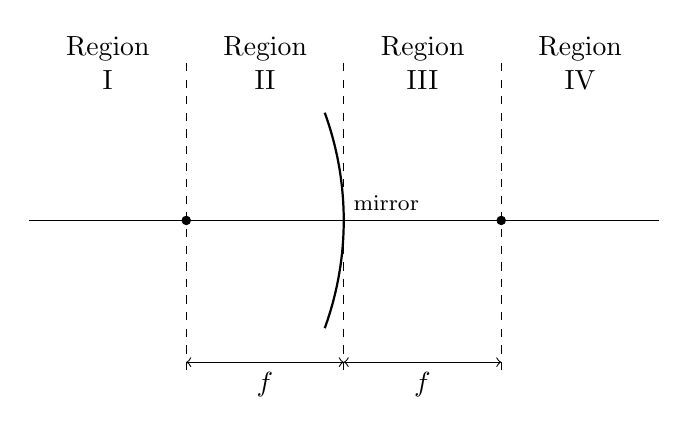
\begin{tikzpicture}
        %% Optical axis
        \draw (-4,0) -- (4,0);
        \draw[fill] (-2,0) circle (1.5pt);
        \draw[fill] (+2,0) circle (1.5pt);
        %% Region Labels
        \node[anchor=center,text width=3em,text centered] at (-3,2) {Region I};
        \node[anchor=center,text width=3em,text centered] at (-1,2) {Region II};
        \node[anchor=center,text width=3em,text centered] at (+1,2) {Region III};
        \node[anchor=center,text width=3em,text centered] at (+3,2) {Region IV};
        %% Region lines
        \draw[dashed] (2,2) -- (2,-2);
        \draw[dashed] (0,2) -- (0,-2);
        \draw[dashed] (-2,2) -- (-2,-2);
        %% Mirror
        \draw[thick] (-4,0) ++ (-20:4) arc (-20:20:4);
        \node[font=\footnotesize,anchor=south west] at (0,0) {mirror};
        %% Focal Lengths
        \draw[<->] (-2,-1.8) -- (0,-1.8) node[pos=0.5,anchor=north] {$f$};
        \draw[<->] (+2,-1.8) -- (0,-1.8) node[pos=0.5,anchor=north] {$f$};
    \end{tikzpicture}
    \end{center}
    A real object now is placed to the left of the mirror.
    In theory, which one of the following choices best describes everywhere that it is impossible for an image to form from the mirror?
    \begin{choices}
      \correctchoice{Region II only.}
        \wrongchoice{Region II and III only.}
        \wrongchoice{Region III and IV only.}
        \wrongchoice{Region II and IV only.}
        \wrongchoice{Region I, II, and IV only.}
    \end{choices}
\end{question}
}

\element{aapt}{ %% Bowl-C2
\begin{question}{bowl-2014-q37}
    A new element is discovered and named PhysicsBowlium (atomic symbol \emph{Phys}).
    Its entry onto the standard periodic table of elements appears as in the figure
        (with Helium shown as well).
    \begin{center}
    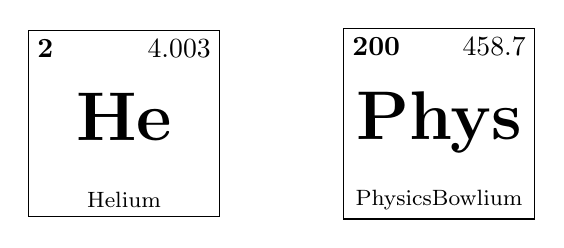
\begin{tikzpicture}
        \node[draw,rectangle,anchor=center] at (-2,0) {
            \begin{minipage}{2.2cm}
                \centering
                {\textbf{2} \hfill 4.003}
                \linebreak \linebreak
                {\Huge\textbf{He}}
                \linebreak \linebreak
                {{\footnotesize Helium}}
            \end{minipage}
        };
        \node[draw,rectangle,anchor=center] at (+2,0) {
            \begin{minipage}{2.2cm}
                \centering
                {\textbf{200} \hfill 458.7}
                \linebreak \linebreak
                {\Huge\textbf{Phys}}
                \linebreak \linebreak
                {{\footnotesize PhysicsBowlium}}
            \end{minipage}
        };
    \end{tikzpicture}
    \end{center}
    Given a sample of \emph{Phys} which acts as a perfect monatomic ideal gas,
        what is the root-mean-square speed of the atoms of the gas if
        the sample is at \SI{20}{\degreeCelsius}?
    \begin{multicols}{3}
    \begin{choices}
        \wrongchoice{\SI{1.04}{\meter\per\second}}
        \wrongchoice{\SI{4.00}{\meter\per\second}}
        \wrongchoice{\SI{33.0}{\meter\per\second}}
      \correctchoice{\SI{126}{\meter\per\second}}
        \wrongchoice{\SI{191}{\meter\per\second}}
    \end{choices}
    \end{multicols}
\end{question}
}

\element{aapt}{ %% Bowl-D2
\begin{question}{bowl-2014-q38}
    In the circuit shown, the switch $S$ has been left open for a very long time.
    \begin{center}
    \ctikzset{bipoles/length=0.75cm}
    \begin{circuitikz}[scale=1.00]
        \draw (0,0) to [battery,l=\SI{9}{\volt}] (0,2) to [R,l=\SI{3}{\kilo\ohm}] (2,2) to [R,l=\SI{1}{\kilo\ohm}] (4,2) to (4,0);
        \draw (0,0) to (2,0) to [C,l=\SI{10}{\micro\farad}] (4,0);
        \draw (2,0) to [cspst,l=$S$] (2,2);
    \end{circuitikz}
    \end{center}
    All circuit elements are considered to be ideal.
    Which one of the following statements best describes the behavior of the current
        through the switch $S$ once it is closed?
    \begin{choices}
      \correctchoice{The current initially is \SI{12}{\milli\ampere} and decreases to a steady \SI{3}{\milli\ampere}.}
        \wrongchoice{The current initially is \SI{3}{\milli\ampere} and increases to a steady \SI{12}{\milli\ampere}.}
        \wrongchoice{The current initially is \SI{9}{\milli\ampere} and decreases to a steady \SI{3}{\milli\ampere}.}
        \wrongchoice{The current initially is \SI{6}{\milli\ampere} and decreases to a steady \SI{3}{\milli\ampere}.}
        \wrongchoice{The current is a steady \SI{3}{\milli\ampere}.}
    \end{choices}
\end{question}
}

\element{aapt}{ %% Bowl-A6
\begin{question}{bowl-2014-q39}
    Two uniform disks, $X$ and $Y$, have masses $m_X < m_Y$, equal radii,
        and equal initial non-zero kinetic energies.
    \begin{center}
    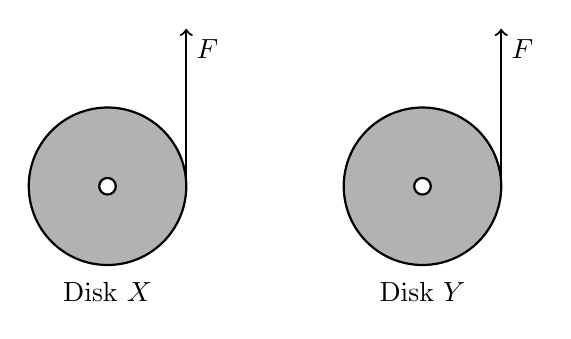
\begin{tikzpicture}
        %% Disk X, on left
        \draw[thick,fill=white!70!black] (-2,0) circle (1.00);
        \draw[thick,fill=white] (-2,0) circle (3pt);
        \draw[thick,->] (-1.00,0) -- ++ (90:2cm)
            node[pos=1.0,anchor=north west] {$F$};
        \node[anchor=north] at (-2,-1.10) {Disk $X$};
        %% Disk Y, on right
        \draw[thick,fill=white!70!black] (+2,0) circle (1.00);
        \draw[thick,fill=white] (+2,0) circle (3pt);
        \draw[thick,->] (3.00,0) -- ++ (90:2cm)
            node[pos=1.0,anchor=north west] {$F$};
        \node[anchor=north] at (+2,-1.10) {Disk $Y$};
    \end{tikzpicture}
    \end{center}
    Each disk rotates counterclockwise in the plane of the page about a
        fixed edge for the same amount of time.
    After the forces are applied, let $L$ represent the magnitude of the
        angular momentum about the center of a disk and $K$ represent the
        kinetic energy of a disk.
    Which one of the following choices correctly compares these quantities
        for disk $X$ and disk $Y$?
    \begin{choices}
        \wrongchoice{$L_X>L_Y$; $K_X<K_Y$}
        \wrongchoice{$L_X>L_Y$; $K_X>K_Y$}
        \wrongchoice{$L_X=L_Y$; $K_X=K_Y$}
        \wrongchoice{$L_X<L_Y$; $K_X<K_Y$}
      \correctchoice{$L_X<L_Y$; $K_X>K_Y$}
    \end{choices}
\end{question}
}

\element{aapt}{ %% Bowl-A2
\begin{question}{bowl-2014-q40}
    A small \SI{1.35}{\kilo\gram} mass is launched from the top of a cliff at an angle of \ang{15.9} above the horizontal.
    \begin{center}
    \begin{tikzpicture}
        %% Surface
        \draw[thick] (0,3) -- (1,3) -- (1,0) -- (3,0);
        %% Top Arrow
        \coordinate (A) at (1,3.1);
        \draw[fill] (A) circle (1pt);
        \draw[thick,->] (A) -- ++ (15.9:1cm);
        \draw[dashed] (A) -- ++ (0:1cm) node [anchor=south west] {\ang{15.9}};
        %% Bottom Arrow
        \coordinate (B) at (3,0);
        \draw[fill] (B) circle (1pt);
        \draw[thick,->] (B) -- ++ (-34.4:1cm);
        \draw[dashed] (B) -- ++ (0:1cm) node[anchor=north west] {\ang{34.4}};
    \end{tikzpicture}
    \end{center}
    When the mass reaches the ground \SI{4.33}{\second} later,
        its velocity is directed at \ang{34.4} below the horizontal.
    What is the speed of the mass when it reaches the ground?
    Ignore air resistance.
    \begin{multicols}{3}
    \begin{choices}
        \wrongchoice{\SI{60.7}{\meter\per\second}}
      \correctchoice{\SI{54.1}{\meter\per\second}}
        \wrongchoice{\SI{46.4}{\meter\per\second}}
        \wrongchoice{\SI{43.3}{\meter\per\second}}
        \wrongchoice{\SI{38.8}{\meter\per\second}}
    \end{choices}
    \end{multicols}
\end{question}
}


%% PhysicsBowl 2014 Division 02 only
%%----------------------------------------
\element{aapt}{ %% Bowl-E2
\begin{question}{bowl-2014-q41}
    ``No two electrons in an atom can have an identical set of
        the four quantum numbers.'' is a statement most closely
        associated with which of the following scientists?
    \begin{multicols}{2}
    \begin{choices}
        \wrongchoice{Albert Einstein}
        \wrongchoice{Enrico Fermi}
        \wrongchoice{Sheldon Cooper}
      \correctchoice{Wolfgang Pauli}
        \wrongchoice{Issac Newton}
    \end{choices}
    \end{multicols}
\end{question}
}

\element{aapt}{ %% Bowl-B3
\begin{question}{bowl-2014-q42}
    Plane-polarized light with intensity $I$ is incident on a single polarizing sheet.
    If the intensity of the light becomes $\frac{1}{4}I$ after passing through the polarizer,
        what is the angle between the transmission axis of the polarizer and the polarizer and the polarization plane of the incident light?
    \begin{multicols}{3}
    \begin{choices}
        \wrongchoice{\ang{75}}
        \wrongchoice{\ang{67.5}}
      \correctchoice{\ang{60}}
        \wrongchoice{\ang{30}}
        \wrongchoice{\ang{22.5}}
    \end{choices}
    \end{multicols}
\end{question}
}

\element{aapt}{ %% Bowl-A6
\begin{question}{bowl-2014-q43}
    A long rod of length $L$ is pivoted about its left end.
    It is released from an angle $\theta$ above the horizontal.
    \begin{center}
    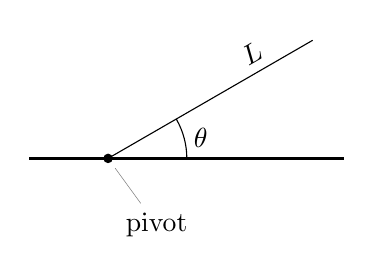
\begin{tikzpicture}
        \draw[line width=1.2pt] (-1,0) -- (3,0);
        \draw[fill] (0,0) circle (1.5pt) node[pin=280:pivot] {};
        \draw (0,0) -- ++ (30:3) node[pos=0.75,anchor=south,rotate=30] {$L$};
        \draw (0:1cm) arc (0:30:1cm) node[pos=0.5,anchor=west] {$\theta$};
    \end{tikzpicture}
    \end{center}
    What is the magnitude of the angular acceleration of the rod about the pivot when the rod is released?
    \begin{multicols}{3}
    \begin{choices}
        \wrongchoice{$\dfrac{6g}{L}\cos\theta$}
        \wrongchoice{$\dfrac{6g}{L}\sin\theta$}
        \wrongchoice{$\dfrac{3g}{L}\sin\theta$}
      \correctchoice{$\dfrac{3g}{L}\cos\theta$}
        \wrongchoice{$\dfrac{3g}{L}\sin\theta$}
    \end{choices}
    \end{multicols}
\end{question}
}

\element{aapt}{ %% Bowl-B2
\begin{question}{bowl-2014-q44}
    A ray of monochromatic light enters the right-triangular glass as shown.
    \begin{center}
    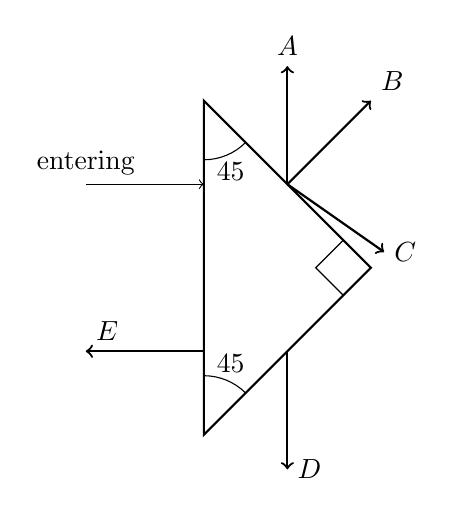
\begin{tikzpicture}[scale=0.75]
        %% Define corners of prism
        \coordinate (A) at (0,0);
        \coordinate (B) at (0,5.656);
        \coordinate (C) at (2.828,2.828);
        \draw[thick] (A) -- (B) -- (C) -- cycle;
        %% Angle labels
        \draw (A) ++ (45:1.00) arc (45:90:1.00) node[pos=0.4,anchor=south] {\ang{45}};
        \draw (B) ++ (270:1.00) arc (270:315:1.00) node[pos=0.6,anchor=north] {\ang{45}};
        \draw (C) ++ (225:0.66) -- ++ (135:0.66) -- ++ (45:0.66);
        %% Entering
        \draw[<-] (B) ++ (270:1.414cm) -- ++ (180:2cm) node[pos=1.0,anchor=south] {entering};
        %% Options
        \draw[thick,->] (B) ++ (-45:2cm) -- ++ (90:2cm) node[pos=1.0,anchor=south] {$A$};
        \draw[thick,->] (B) ++ (-45:2cm) -- ++ (45:2cm) node[pos=1.0,anchor=south west] {$B$};
        \draw[thick,->] (B) ++ (-45:2cm) -- ++ (-35:2cm) node[pos=1.0,anchor=west] {$C$};
        \draw[thick,->] (A) ++ (45:2cm) -- ++ (270:2cm) node[pos=1.0,anchor=west] {$D$};
        \draw[thick,->] (A) ++ (90:1.414cm) -- ++ (180:2cm) node[pos=1.0,anchor=south west] {$E$};
    \end{tikzpicture}
    \end{center}
    %% NOTE: critical angle for crown glass is 41 = asin( 1/1.52 )
    Which one of the lettered rays shows the path of the light after it exits the glass?
    \begin{multicols}{5}
    \begin{choices}[o]
        \wrongchoice{$A$}
        \wrongchoice{$B$}
        \wrongchoice{$C$}
        \wrongchoice{$D$}
      \correctchoice{$E$}
    \end{choices}
    \end{multicols}
\end{question}
}

\element{aapt}{ %% Bowl-A8
\begin{question}{bowl-2014-q45}
    A long thin rod of mass $M$ and length $L$ is pivoted at one end so that it swings as a pendulum.
    The rod is set into simple harmonic oscillation and has a period of motion $T$.
    A second thin rod with mass $2M$ and length $2L$ also is pivoted at one end to swing as a pendulum.
    When this second rod is set into simple harmonic oscillation,
        what is its period?
    \begin{multicols}{3}
    \begin{choices}
        \wrongchoice{$2T$}
      \correctchoice{$\sqrt{2}T$}
        \wrongchoice{$T$}
        \wrongchoice{$\dfrac{1}{\sqrt{2}}T$}
        \wrongchoice{$\dfrac{1}{2}T$}
    \end{choices}
    \end{multicols}
\end{question}
}

\element{aapt}{ %% Bowl-C3
\begin{question}{bowl-2014-q46}
    A monatomic, ideal gas undergoes an isobaric process.
    During the process,
        the gas performs \SI{80}{\joule} of work on the surrounding.
    Which one of the following statements best describes the head exchange during this process?
    \begin{choices}
      \correctchoice{\SI{200}{\joule} of energy was added to the gas.}
        \wrongchoice{\SI{200}{\joule} of energy was removed from the gas.}
        \wrongchoice{\SI{80}{\joule} of energy was added to the gas.}
        \wrongchoice{\SI{80}{\joule} of energy was removed from the gas.}
        \wrongchoice{It cannot be determined without knowing the change in temperature for the gas.}
    \end{choices}
\end{question}
}

\element{aapt}{ %% Bowl-D1
\begin{question}{bowl-2014-q47}
    An air-filled parallel plate capacitor of capacitance $C$ is fully charged after being connected to a battery of voltage $V$.
    The battery then is disconnected and an insulating dielectric slave of constant $\kappa$ is inserted between the capacitor's plates,
        fully filling the region.
    What is the voltage between the plates once equilibrium is established with the dielectric in place?
    \begin{multicols}{3}
    \begin{choices}
        \wrongchoice{$\kappa^2V$}
        \wrongchoice{$\kappa V$}
        \wrongchoice{$V$}
      \correctchoice{$\dfrac{V}{\kappa}$}
        \wrongchoice{$\dfrac{V}{\kappa^2}$}
    \end{choices}
    \end{multicols}
\end{question}
}

\element{aapt}{ %% Bowl-B3
\begin{question}{bowl-2014-q48}
    A laser beam with wavelength \SI{632.8}{\nano\meter} shines onto a newly fabricated single slit.
    As a result, the width of the principal bright region on a viewing screen \SI{1.25}{\meter} away is \SI{1.00}{\meter}.
    Which of the following best represents the size of the single slit opening?
    \begin{multicols}{3}
    \begin{choices}
        \wrongchoice{\SI{0.79}{\micro\meter}}
        \wrongchoice{\SI{0.85}{\micro\meter}}
        \wrongchoice{\SI{1.01}{\micro\meter}}
        \wrongchoice{\SI{1.58}{\micro\meter}}
      \correctchoice{\SI{1.70}{\micro\meter}}
    \end{choices}
    \end{multicols}
\end{question}
}

\element{aapt}{ %% Bowl-A6
\begin{question}{bowl-2014-q49}
    A solid, uniform disk of mass $M$ and radius $R$ rotates clockwise about its center with an angular speed $\omega_0$.
    \begin{center}
    \begin{tikzpicture}
        %% Surface
        \draw (-2,0) -- (2,0);
        \node[anchor=north,pattern=north east lines,minimum width=4cm,minimum height=0.05cm] at (0,0) {};
        %% Circle
        \draw (0,1) circle (1cm);
        \draw[thick,->] (0,1) -- ++ (225:1cm) node[pos=0.5,anchor=south east] {$R$};
        \draw[thick,->] (0,1) ++ (125:0.5cm) arc(125:-45:0.5cm);
        \draw (0,1) ++ (135:1.1cm) node[anchor=south] {$M$};
    \end{tikzpicture}
    \end{center}
    The disk then is placed onto a horizontal surface and beings moving only to the right, slipping as it rolls.
    The coefficient of friction between the floor and the disk is $\mu$ and the frictional force is considered constant throughout the motion.
    What is the angular speed of the disk when the disk starts rolling without slipping?
    \begin{multicols}{3}
    \begin{choices}
        \wrongchoice{$\dfrac{\mu}{2}\omega_0$}
        \wrongchoice{$\dfrac{1}{2}\omega_0$}
      \correctchoice{$\dfrac{1}{3}\omega_0$}
        \wrongchoice{$\dfrac{2\mu}{3}\omega_0$}
        \wrongchoice{$\dfrac{3}{5}\omega_0$}
    \end{choices}
    \end{multicols}
\end{question}
}

\element{aapt}{ %% Bowl-E3
\begin{question}{bowl-2014-q50}
    Two clocks, $A$ and $B$, are synchronized on Earth.
    Clock $A$ is placed onto a space ship that leaves Earth in a straight line with speed of \SI{2.40e8}{\meter\per\second}.
    On Earth, a scientist with clock $B$ has her telescope fixed directly on clock $A$.
    If each clock started at $t=\SI{0}{\second}$,
        what time does the scientist observe on clock $A$ when clock $B$ reads $t=\SI{90}{\second}$?
    Assume the time of acceleration for the ship leaving the Earth was negligible.
    \begin{multicols}{3}
    \begin{choices}
        \wrongchoice{\SI{24}{\second}}
      \correctchoice{\SI{30}{\second}}
        \wrongchoice{\SI{50}{\second}}
        \wrongchoice{\SI{54}{\second}}
        \wrongchoice{\SI{72}{\second}}
    \end{choices}
    \end{multicols}
\end{question}
}


%% PhysicsBowl 2013 Division 01 only
%%----------------------------------------
\element{aapt}{ %% Bowl-M1
\begin{question}{bowl-2013-q01}
    Red light from a laser is noted to have a wavelength of \SI{632.8}{\nano\meter}.
    Which one of the following choices best represents the meaning of the prefix \emph{nano}?
    \begin{multicols}{3}
    \begin{choices}
        \wrongchoice{\num{e-3}}
        \wrongchoice{\num{e-6}}
      \correctchoice{\num{e-9}}
        \wrongchoice{\num{e-12}}
        \wrongchoice{\num{e-15}}
    \end{choices}
    \end{multicols}
\end{question}
}

\element{aapt}{ %% Bowl-A2
\begin{question}{bowl-2013-q02}
    A small object is released from rest and reaches the ground in a time of \SI{2.50}{\second}.
    With what speed does the object reach the ground?
    Neglect air resistance.
    \begin{multicols}{3}
    \begin{choices}
        \wrongchoice{\SI{31.3}{\meter\per\second}}
      \correctchoice{\SI{25.0}{\meter\per\second}}
        \wrongchoice{\SI{12.5}{\meter\per\second}}
        \wrongchoice{\SI{10.0}{\meter\per\second}}
        \wrongchoice{\SI{2.50}{\meter\per\second}}
    \end{choices}
    \end{multicols}
\end{question}
}

\element{aapt}{ %% Bowl-A2
\begin{question}{bowl-2013-q03}
    A small object is released from rest and reaches the ground in a time of \SI{2.50}{\second}.
    From what height above the ground was the object being released?
    Neglect air resistance.
    \begin{multicols}{3}
    \begin{choices}
        \wrongchoice{\SI{6.25}{\meter}}
        \wrongchoice{\SI{12.5}{\meter}}
        \wrongchoice{\SI{25.0}{\meter}}
      \correctchoice{\SI{31.3}{\meter}}
        \wrongchoice{\SI{62.5}{\meter}}
    \end{choices}
    \end{multicols}
\end{question}
}

\element{aapt}{ %% Bowl-??
\begin{question}{bowl-2013-q04}
    A scientist calculated a quantity that was equal to one light-year.
    Which one of the following choices represents the type of quantity that the scientist calculated?
    \begin{multicols}{3}
    \begin{choices}
        \wrongchoice{Time}
        \wrongchoice{Mass}
        \wrongchoice{Speed}
        \wrongchoice{Force}
      \correctchoice{Distance}
    \end{choices}
    \end{multicols}
\end{question}
}

\element{aapt}{ %% Bowl-A5
\begin{question}{bowl-2013-q05}
    At an instant of time $t$, a point object of mass $M$ moves with velocity $\vec{V}$,
        has acceleration $\vec{A}$, and is at position $(x,y)$.
    In what direction must the linear momentum of the object be directed at this instant?
    \begin{choices}
      \correctchoice{Along the direction of the velocity of the mass.}
        \wrongchoice{Along the direction of the net force acting on the mass.}
        \wrongchoice{Along the direction of the vector from the origin $(0,0)$ to $(x,y)$.}
        \wrongchoice{Along the direction of the acceleration of the mass.}
        \wrongchoice{Along the direction perpendicular to the object's acceleration.}
    \end{choices}
\end{question}
}

\element{aapt}{ %% Bowl-A8
\begin{question}{bowl-2013-q06}
    A \SI{1.50}{\meter} long string clamped at both ends is vibrating at its second harmonic.
    What is the wavelength associated with the string for this scenario?
    \begin{multicols}{3}
    \begin{choices}
        \wrongchoice{\SI{3.00}{\meter}}
        \wrongchoice{\SI{2.25}{\meter}}
      \correctchoice{\SI{1.50}{\meter}}
        \wrongchoice{\SI{1.00}{\meter}}
        \wrongchoice{\SI{0.75}{\meter}}
    \end{choices}
    \end{multicols}
\end{question}
}

\element{aapt}{ %% Bowl-D1
\begin{question}{bowl-2013-q07}
    Two identical particles are fixed in place a distance of \SI{0.50}{\meter} apart.
    The electric force that one particle exerts on the other has a magnitude of \SI{3.00}{\newton}.
    Which one of the following choices best represents the magnitude of each particle's charge?
    \begin{multicols}{2}
    \begin{choices}
        \wrongchoice{\SI{4.17e-11}{\coulomb}}
        \wrongchoice{\SI{8.33e-11}{\coulomb}}
        \wrongchoice{\SI{1.67e-10}{\coulomb}}
      \correctchoice{\SI{9.13e-6}{\coulomb}}
        \wrongchoice{\SI{1.29e-5}{\coulomb}}
    \end{choices}
    \end{multicols}
\end{question}
}

\element{aapt}{ %% Bowl-??
\begin{question}{bowl-2013-q08}
    Some standard household lights are being replaced with LEDs.
    LED is the acronym for which one of the following choice?
    \begin{choices}
        \wrongchoice{Low Emission Dial}
      \correctchoice{Light Emitting Diode}
        \wrongchoice{Light Energy Divider}
        \wrongchoice{Lower Edge Disc}
        \wrongchoice{Limiting Emission Diode}
    \end{choices}
\end{question}
}

\element{aapt}{ %% Bowl-A8
\begin{question}{bowl-2013-q09}
    A simple pendulum oscillated with period of \SI{2.0}{\second}.
    \begin{center}
    \begin{tikzpicture}
        \draw[dashed] (0,0) -- ++ (270:3cm);
        \draw[thick] (0,0) -- ++ (240:3cm);
        \draw[fill] (240:3cm) circle (3pt);
        \draw[dashed] (300:3cm) arc (300:240:3cm);
        \draw[<-] (240:1cm) arc (240:270:1cm)
            node[font=\small,anchor=north,pos=0.5] {\ang{4}};
    \end{tikzpicture}
    \end{center}
    If the maximum oscillation of the pendulum is \ang{4.0} from equilibrium,
        what is the length of the string for this pendulum?
    \begin{multicols}{3}
    \begin{choices}
        \wrongchoice{\SI{6.4}{\meter}}
        \wrongchoice{\SI{3.2}{\meter}}
        \wrongchoice{\SI{1.6}{\meter}}
      \correctchoice{\SI{1.0}{\meter}}
        \wrongchoice{\SI{0.5}{\meter}}
    \end{choices}
    \end{multicols}
\end{question}
}

\element{aapt}{ %% Bowl-A2
\begin{question}{bowl-2013-q10}
    An object is thrown straight upward.
    The object remains in free fall until it returns to its initial launch point.
    Which one of the following graphs could represent the velocity of the object as a function of time during the flight?
    \begin{multicols}{2}
    \begin{choices}
        \AMCboxDimensions{down=-2.0em}
        \wrongchoice{
            \begin{tikzpicture}
                \begin{axis}[
                    axis y line=left,
                    axis x line=middle,
                    axis line style={->},
                    xlabel={time},
                    xtick=\empty,
                    x label style={anchor=north east},
                    ylabel={velocity},
                    ytick=\empty,
                    xmin=0,xmax=11,
                    ymin=-5.5,ymax=5.5,
                    width=0.95\columnwidth,
                    very thin,
                ]
                \addplot[line width=1pt,domain=0:5]{5-x};
                \addplot[line width=1pt,domain=5:10]{(x-5)};
                \end{axis}
            \end{tikzpicture}
        }
        \wrongchoice{
            \begin{tikzpicture}
                \begin{axis}[
                    axis y line=left,
                    axis x line=middle,
                    axis line style={->},
                    xlabel={time},
                    xtick=\empty,
                    x label style={anchor=south east},
                    ylabel={velocity},
                    ytick=\empty,
                    xmin=0,xmax=11,
                    ymin=-5.5,ymax=5.5,
                    width=0.95\columnwidth,
                    very thin,
                ]
                \addplot[line width=1pt,domain=0:5]{-5+x};
                \addplot[line width=1pt,domain=5:10]{(5-x)};
                \end{axis}
            \end{tikzpicture}
        }
        \wrongchoice{
            \begin{tikzpicture}
                \begin{axis}[
                    axis y line=left,
                    axis x line=middle,
                    axis line style={->},
                    xlabel={time},
                    xtick=\empty,
                    x label style={anchor=north east},
                    ylabel={velocity},
                    ytick=\empty,
                    xmin=0,xmax=11,
                    ymin=-5.5,ymax=5.5,
                    width=0.95\columnwidth,
                    very thin,
                ]
                \addplot[line width=1pt,domain=0:10]{0.2*(x-5)*(x-5)};
                \end{axis}
            \end{tikzpicture}
        }
        \wrongchoice{
            \begin{tikzpicture}
                \begin{axis}[
                    axis y line=left,
                    axis x line=middle,
                    axis line style={->},
                    xlabel={time},
                    xtick=\empty,
                    x label style={anchor=south east},
                    ylabel={velocity},
                    ytick=\empty,
                    xmin=0,xmax=11,
                    ymin=-5.5,ymax=5.5,
                    width=0.95\columnwidth,
                    very thin,
                ]
                \addplot[line width=1pt,domain=0:10]{-0.2*(x-5)*(x-5)};
                \end{axis}
            \end{tikzpicture}
        }
        \correctchoice{
            \begin{tikzpicture}
                \begin{axis}[
                    axis y line=left,
                    axis x line=middle,
                    axis line style={->},
                    xlabel={time},
                    xtick=\empty,
                    x label style={anchor=south east},
                    ylabel={velocity},
                    ytick=\empty,
                    xmin=0,xmax=11,
                    ymin=-5.5,ymax=5.5,
                    width=0.95\columnwidth,
                    very thin,
                ]
                \addplot[line width=1pt,domain=0:10]{5-x};
                \end{axis}
            \end{tikzpicture}
        }
    \end{choices}
    \end{multicols}
\end{question}
}


%% PhysicsBowl 2013 Division 01 and 02
%%----------------------------------------
\element{aapt}{ %% Bowl-??
\begin{question}{bowl-2013-q11}
    There was great excitement in the physics community because of an announcement from the LHC during the summer of 2012.
    Which one of the following choices best represents the reason for the excitement?
    \begin{choices}
        \wrongchoice{The announcement that life was found on Mars.}
        \wrongchoice{The announcement that dark matter had been created and studied in the laboratory.}
        \wrongchoice{The announcement that the Hubble Telescope discovered a ``spaceship-like'' object near Alpha Centauri.}
        \wrongchoice{The announcement that the mass of a neutrino had been determined.}
      \correctchoice{The announcement that there was experimental evidence of a particle consistent with a Higgs Boson.}
    \end{choices}
\end{question}
}

\element{aapt}{ %% Bowl-A7
\begin{question}{bowl-2013-q12}
    It takes the Earth one day to rotate about its axis.
    Which one of the following choices best represents the time that it takes the Moon to make one rotation about its axis?
    \begin{choices}
        \wrongchoice{One day.}
        \wrongchoice{One week.}
      \correctchoice{One month.}
        \wrongchoice{One year.}
        \wrongchoice{It does not rotate at all.}
    \end{choices}
\end{question}
}

\element{aapt}{ %% Bowl-M1
\begin{question}{bowl-2013-q13}
    Which one of the following choices represents the measurement with the most number of significant digits?
    \begin{multicols}{2}
    \begin{choices}
        \wrongchoice{\SI{6.75}{\meter}}
        \wrongchoice{\SI{4.67e9}{\meter}}
        \wrongchoice{\SI{0.000 000 012}{\meter}}
        \wrongchoice{\SI{8100}{\meter}}
      \correctchoice{\SI{2.000 05}{\meter}}
    \end{choices}
    \end{multicols}
\end{question}
}

\element{aapt}{ %% Bowl-A2
\begin{question}{bowl-2013-q14}
    A small box is thrown at an angle of \ang{30.0} above the horizontal ground with a speed of \SI{20.0}{\meter\per\second}.
    To what maximum height above the launch point does the ball rise during its motion?
    Ignore air resistance.
    \begin{multicols}{3}
    \begin{choices}
        \wrongchoice{\SI{2.5}{\meter}}
      \correctchoice{\SI{5.0}{\meter}}
        \wrongchoice{\SI{10.0}{\meter}}
        \wrongchoice{\SI{15.0}{\meter}}
        \wrongchoice{\SI{20.0}{\meter}}
    \end{choices}
    \end{multicols}
\end{question}
}

\element{aapt}{ %% Bowl-D2
\begin{question}{bowl-2013-q15}
    In a circuit, the flow of electrons in a horizontal wire produces a constant current of \SI{3.2}{\ampere} for a time of \SI{3.0}{\hour}.
    Which one of the following choices best represents the number of electrons that pass through a vertical cross-section of the wire during this time?
    \begin{multicols}{2}
    \begin{choices}
        \wrongchoice{\num{9.60}}
        \wrongchoice{\num{6.00e19}}
        \wrongchoice{\num{7.20e22}}
      \correctchoice{\num{2.16e23}}
        \wrongchoice{\num{6.02e23}}
    \end{choices}
    \end{multicols}
\end{question}
}

\element{aapt}{ %% Bowl-A3
\begin{question}{bowl-2013-q16}
    A block initially moving at \SI{8.0}{\meter\per\second} accelerates uniformly to rest on a horizontal surface.
    The block travels a distance of \SI{12.0}{\meter} during the slide.
    Which one of the following choices best represents the coefficient of kinetic friction between the surface and the block?
    \begin{multicols}{3}
    \begin{choices}
        \wrongchoice{\num{1.20}}
        \wrongchoice{\num{0.667}}
        \wrongchoice{\num{0.533}}
      \correctchoice{\num{0.267}}
        \wrongchoice{\num{0.133}}
    \end{choices}
    \end{multicols}
\end{question}
}

\element{aapt}{ %% Bowl-A1
\begin{question}{bowl-2013-q17}
    A position vs. time graph of a particle moving along a horizontal axis is shown.
    \begin{center}
    \begin{tikzpicture}
        \begin{axis}[
            axis y line=left,
            axis x line=middle,
            axis line style={->},
            xlabel={time},
            x unit=\si{\second},
            xtick={0,2,4,6,8,10},
            minor xtick={1,3,5,7,9},
            ylabel={position},
            y unit=\si{\meter},
            ytick={-10,0,10},
            minor ytick={-8,-6,-4,-2,2,4,6,8},
            grid=both,
            xmin=0,xmax=10.5,
            ymin=-10.5,ymax=10.5,
            width=0.95\columnwidth,
            height=0.618\columnwidth,
        ]
        \addplot[line width=1pt,mark=\empty] plot coordinates { (0,8) (3,8) (5,0) (6,0) (8,-8) (9,-8) (10,10) };
        \end{axis}
    \end{tikzpicture}
    \end{center}
    What is the total distance traveled by the particle from $t=\SI{0}{\second}$ to $t=\SI{10}{\second}$?
    \begin{multicols}{3}
    \begin{choices}
        \wrongchoice{\SI{2}{\meter}}
        \wrongchoice{\SI{18}{\meter}}
        \wrongchoice{\SI{26}{\meter}}
      \correctchoice{\SI{34}{\meter}}
        \wrongchoice{\SI{42}{\meter}}
    \end{choices}
    \end{multicols}
\end{question}
}

\element{aapt}{ %% Bowl-A2
\begin{questionmult}{bowl-2013-q18}
    Which of the following choices correctly identifies a situations for which there is a non-zero acceleration?
    \begin{choices}
      \correctchoice{A point object moves in a straight line with increasing speed.}
      \correctchoice{A point object moves in a circular path with constant speed.}
      \correctchoice{A point object moves in a circular path with decreasing speed.}
    \end{choices}
\end{questionmult}
}

\element{aapt}{ %% Bowl-??
\begin{question}{bowl-2013-q19}
    Which physicist won the Nobel Prize in physics partly for the explanation of the photoelectric effect?
    \begin{multicols}{2}
    \begin{choices}
        \wrongchoice{Isaac Newton}
        \wrongchoice{Steven Hawing}
      \correctchoice{Albert Einstein}
        \wrongchoice{Marie Curie}
        \wrongchoice{Neil deGrasse Tyson}
    \end{choices}
    \end{multicols}
\end{question}
}

\element{aapt}{ %% Bowl-C2
\begin{question}{bowl-2013-q20}
    A sample of ideal gas at a temperature of \SI{40.0}{\degreeCelsius} is in a container of volume \SI{3.50e-2}{\meter\cubed}.
    If the pressure of the gas is \SI{0.50}{\atm},
        how many molecules of the gas are in the container?
    \begin{multicols}{2}
    \begin{choices}
        \wrongchoice{\num{4.05e18}}
        \wrongchoice{\num{4.10e20}}
        \wrongchoice{\num{4.05e21}}
      \correctchoice{\num{4.10e23}}
        \wrongchoice{\num{4.10e26}}
    \end{choices}
    \end{multicols}
\end{question}
}

\element{aapt}{ %% Bowl-E2
\begin{question}{bowl-2013-q21}
    The following nuclear reaction occurs:
    \begin{equation}
        \ce{^{131}_{53}I -> ^{131}_{54}Xe + ^{A}_{Z}X}
    \end{equation}
    What is \ce{^{A}_{Z}X}?
    \begin{multicols}{2}
    \begin{choices}
        \wrongchoice{a neutron}
        \wrongchoice{a proton}
        \wrongchoice{a positron}
        \wrongchoice{an alpha particle}
      \correctchoice{an electron}
    \end{choices}
    \end{multicols}
\end{question}
}

\element{aapt}{ %% Bowl-D2
\begin{question}{bowl-2013-q22}
    Four resistors, each of resistance $R$,
        are connected to a battery in the following way: ``Two resistors are connected in series.
    This combination of two resistors is connected in parallel to a third resistor.
    This set of three resistors is connected in series to a fourth resistor.''
    What is the equivalent resistance of this arrangement of four resistors?
    \begin{multicols}{3}
    \begin{choices}
        \wrongchoice{$\dfrac{5}{2}R$}
      \correctchoice{$\dfrac{5}{3}R$}
        \wrongchoice{$\dfrac{4}{3}R$}
        \wrongchoice{$\dfrac{3}{5}R$}
        \wrongchoice{$\dfrac{2}{5}R$}
    \end{choices}
    \end{multicols}
\end{question}
}

\element{aapt}{ %% Bowl-A6
\begin{question}{bowl-2013-q23}
    A small object of mass \SI{11.0}{\gram} is at rest \SI{30.0}{\centi\meter} from a horizontal disk's center.
    The disk starts to rotate from rest about its center with a constant angular acceleration of \SI{4.50}{\radian\per\second\squared}.
    What is the magnitude of the net force acting on the object after a time of $t=\SI{1/3}{\second}$ if the object remains at rest with respect to the disk?
    \begin{multicols}{2}
    \begin{choices}
        \wrongchoice{\SI{0}{\newton}}
        \wrongchoice{\SI{7.43e-3}{\newton}}
        \wrongchoice{\SI{1.49e-2}{\newton}}
      \correctchoice{\SI{1.66e-2}{\newton}}
        \wrongchoice{\SI{2.23e-2}{\newton}}
    \end{choices}
    \end{multicols}
\end{question}
}

\element{aapt}{ %% Bowl-B3
\begin{question}{bowl-2013-q24}
    Which one of the following statements best describes Huygens' Principle?
    \begin{choices}
        \wrongchoice{An additional pressure is transmitted undiminished to all points in the fluid and to the walls of the container.}
      \correctchoice{Each point on a wavefront acts as a source of secondary spherical wavelets (new waves).}
        \wrongchoice{For every action force, there is an equal but opposite reaction force.}
        \wrongchoice{It is impossible to have a process which has the sole result of transferring energy from a low temperature reservoir to a high temperature reservoir.}
        \wrongchoice{A time-changing magnetic field has an associated induced electric field.}
    \end{choices}
\end{question}
}

\element{aapt}{ %% Bowl-??
\begin{question}{bowl-2013-q25}
    An ideal fluid completely fills a small horizontal tube that has a narrowing cross-sectional area as seen in the figure.
    \begin{center}
    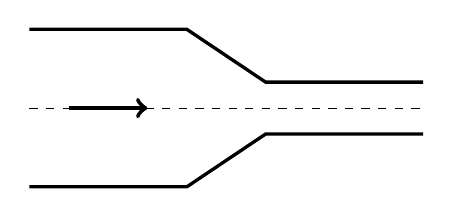
\begin{tikzpicture}
        \draw [dashed] (-2,0) -- (3,0);
        \draw [ultra thick,->] (-1.5,0) -- (-0.5,0);
        \draw [very thick] (-2,+1) -- (0,+1) -- (1,+0.33) -- (3,+0.33);
        \draw [very thick] (-2,-1) -- (0,-1) -- (1,-0.33) -- (3,-0.33);
    \end{tikzpicture}
    \end{center}
    %% changed tense
    Which one of the following choices best describes what will happen to the fluid's speed and the associated pressure in the narrower region as compared to the wider region?
    \begin{choices}
      \correctchoice{The fluid speed increases and the fluid pressure decreases.}
        \wrongchoice{The fluid speed increases and the fluid pressure increases.}
        \wrongchoice{The fluid speed increases and the fluid pressure remained the same.}
        \wrongchoice{The fluid speed decreases and the fluid pressure increases.}
        \wrongchoice{The fluid speed decreases and the fluid pressure decreases.}
    \end{choices}
\end{question}
}

\element{aapt}{ %% Bowl-A1
\begin{question}{bowl-2013-q26}
    An object moving only to the right completes a \SI{20.0}{\second} trip in two stages, I and II.
    The average speed of the entire \SI{20.0}{\second} trip is \SI{10.0}{\meter\per\second}.
    For state I, the object moves with a constant velocity of \SI{6.0}{\meter\per\second} for \SI{12.0}{\second}.
    What constant acceleration must the object have during the \SI{8.0}{\second} of stage II?
    \begin{multicols}{2}
    \begin{choices}
        \wrongchoice{\SI{2.25}{\meter\per\second\squared}}
      \correctchoice{\SI{2.50}{\meter\per\second\squared}}
        \wrongchoice{\SI{4.00}{\meter\per\second\squared}}
        \wrongchoice{\SI{6.25}{\meter\per\second\squared}}
        \wrongchoice{\SI{8.50}{\meter\per\second\squared}}
    \end{choices}
    \end{multicols}
\end{question}
}

\element{aapt}{ %% Bowl-B2
\begin{question}{bowl-2013-q27}
    Light of wavelength \SI{600}{\nano\meter} is transmitted from air into a piece of glass.
    \begin{center}
    \begin{tikzpicture}
    \begin{scope}[decoration={markings,mark=at position 0.66 with {\arrow{latex}}}]
        %% 30, 60 triangle
        \draw[thick] (0,0) -- (-6.93,0) -- (-6.93,4) -- cycle;
        \node[anchor=south west,shift={(1ex,1ex)}] at (-6.93,0) {Glass};
        %% incoming
        \draw[thick,postaction={decorate}] (0,2) -- (-3.46,2);
        %% refracted
        \foreach \x/\y in {160/A,180/B,206/C}
            \draw[thick,postaction={decorate}] (-3.46,2) -- ++ (\x:1.73) node[anchor=center,shift={(\x:1em)}] {$\y$};
        \foreach \x/\y in {270/D,290/E}
            \draw[thick,postaction={decorate}] (-3.46,2) -- ++ (\x:1.41) node[anchor=center,shift={(\x:1em)}] {$\y$};
    \end{scope}
    \end{tikzpicture}
    \end{center}
    Which one of the labeled arrows best indicates the path of the light ray after it enters the glass?
    \begin{multicols}{5}
    \begin{choices}[o]
        \wrongchoice{$A$}
        \wrongchoice{$B$}
      \correctchoice{$C$}
        \wrongchoice{$D$}
        \wrongchoice{$E$}
    \end{choices}
    \end{multicols}
\end{question}
}

\element{aapt}{ %% Bowl-A3
\begin{question}{bowl-2013-q28}
    An object is in free fall close to the ground.
    A person intervenes and slows the object uniformly to rest.
    Which one of the following statements must be true about the magnitude of the acceleration of the object as it is being stopped by the person?
    The magnitude of the object's acceleration is $a_{obj}$ and the magnitude of the acceleration from gravity is $g$.
    \begin{multicols}{2}
    \begin{choices}
        \wrongchoice{$a_{obj} = g$}
        \wrongchoice{$a_{obj} > g$}
        \wrongchoice{$a_{obj} < g$}
        \wrongchoice{$a_{obj} \leq g$}
        \wrongchoice{$a_{obj} \geq g$}
      \correctchoice{None of these relations must be true.}
    \end{choices}
    \end{multicols}
\end{question}
}

\element{aapt}{ %% Bowl-D1
\begin{question}{bowl-2013-q29}
    Two electrons enter a region between charged capacitor plates with equal speed $v$.
    \begin{center}
    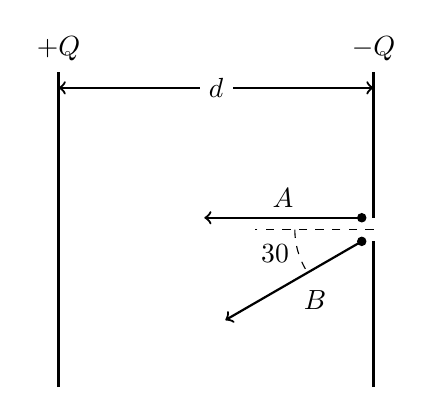
\begin{tikzpicture}
        %% Plates
        \draw[very thick] (-2,-2) -- (-2,+2) node[anchor=south] {$+Q$};
        \draw[very thick] (+2,-2) -- (+2,+2) node[anchor=south] {$-Q$};
        %% Gap
        \fill[white] (+1.9,-0.15) rectangle (+2.1,+0.15);
        %% Distance
        \draw[thick,<->] (-2,1.8) -- (+2,1.8) node[pos=0.5,anchor=center,fill=white] {$d$};
        %% Two electrons A and B
        \coordinate (A) at (1.85,+0.15);
        \coordinate (B) at (1.85,-0.15);
        \draw[fill] (A) circle (1.5pt);
        \draw[fill] (B) circle (1.5pt);
        \draw[thick,->] (A) -- ++ (180:2.0cm) node[pos=0.5,anchor=south] {$A$};
        \draw[thick,->] (B) -- ++ (210:2.0cm) node[pos=0.5,anchor=north west] {$B$};
        %% 30 degrees
        \draw[dashed] (2,0) -- ++ (180:1.5cm);
        \draw[dashed] (2,0) ++ (180:1.0cm) arc (180:210:1.0) node[pos=0.6,anchor=east] {\ang{30}};
    \end{tikzpicture}
    \end{center}
    Electron $A$ is directed horizontally to the left while electron $B$ is directed at \ang{30} below the horizontal.
    Each electron makes it to the left-hand plate.
    Which one of the following choices best compares the speeds of the charges $(v_A,v_B)$ upon arrival at the left plate?
    Consider only the electrons $A$ and $B$'s interactions with the constant electric field between the plates, ignoring any relativistic effects.
    \begin{choices}
        \wrongchoice{$v_A > v_B$}
      \correctchoice{$v_A = v_B$}
        \wrongchoice{$v_A < v_B$}
        \wrongchoice{The answer depends on the size of the plate separation $d$.}
        \wrongchoice{The answer depends on the magnitude of the charge, $Q$, on each plate.}
    \end{choices}
\end{question}
}

\element{aapt}{ %% Bowl-D4
\begin{question}{bowl-2013-q30}
    Electrons flow to the left in a wire as shown.
    \begin{center}
    \begin{tikzpicture}
        %% Wire
        \draw (-3.5,+0.5) -- (+3.5,+0.5);
        \draw (-3.5,-0.5) -- (+3.5,-0.5);
        %% Current
        \foreach \x in {30,20,10,0,-10,-20}
            \draw[xshift=-0.25cm,thick,->] (\x mm,0) -- ++ (180:0.75cm);
        \draw[fill] (3,0) circle (1.5pt)
            node[anchor=west] {$e^-$};
        %% Electron
        \draw[fill] (0,1) circle (1pt)
            node[anchor=west] {$p^+$};
            %node[anchor=west] {proton};
        \draw[thick,->] (0,1) -- ++ (90:1cm)
            node[pos=0.5,anchor=west] {$v$};
    \end{tikzpicture}
    \end{center}
    For the proton moving toward the top of the page at the instant shown,
        what is the direction of the magnetic force on the proton?
    \begin{choices}
        \wrongchoice{To the left}
      \correctchoice{To the right}
        \wrongchoice{Into the plane of the page}
        \wrongchoice{Out of the plane of the page}
        \wrongchoice{There is no force}
    \end{choices}
\end{question}
}

\element{aapt}{ %% Bowl-C3
\begin{question}{bowl-2013-q31}
    A monatomic ideal gas undergoes a reversible isothermal expansion in an enclosed container.
    Which one of the following quantities associated with the gas has a value of \emph{zero}?
    \begin{choices}
        \wrongchoice{Heat}
        \wrongchoice{Entropy change}
        \wrongchoice{Work done}
      \correctchoice{Internal energy change}
        \wrongchoice{Pressure change}
    \end{choices}
\end{question}
}

\element{aapt}{ %% Bowl-A1
\begin{question}{bowl-2013-q32}
    An acceleration vs. time graph for an object moving along a line is shown.
    \begin{center}
    \begin{tikzpicture}
        \begin{axis}[
            axis y line=left,
            axis x line=middle,
            axis line style={->},
            xlabel={time},
            x unit=\si{\second},
            xtick={0,2,4,6,8,10},
            minor xtick={1,3,5,7,9},
            ylabel={acceleration},
            y unit=\si{\meter\per\second\squared},
            ytick={-10,0,10},
            minor ytick={-8,-6,-4,-2,2,4,6,8},
            grid=both,
            xmin=0,xmax=10.25,
            ymin=-10.5,ymax=10.5,
            width=0.95\columnwidth,
            height=0.618\columnwidth,
        ]
        \addplot[line width=1pt,domain=0:10]{8*sin(1.26*deg(x))};
        \end{axis}
    \end{tikzpicture}
    \end{center}
    The object starts from rest at time $t=\SI{0}{\second}$.
    At what time(s) does the object attain a maximum displacement from its starting position?
    \begin{choices}
        \wrongchoice{At times $t=\SI{2.5}{\second}$ and $t=\SI{7.5}{\second}$ only}
        \wrongchoice{At times $t=\SI{5.0}{\second}$ and $t=\SI{10}{\second}$ only}
        \wrongchoice{At times $t=\SI{1.25}{\second}$, $t=\SI{3.75}{\second}$,
            $t=\SI{6.25}{\second}$, and $t=\SI{8.75}{\second}$ only}
        \wrongchoice{At times $t=\SI{2.5}{\second}$, $t=\SI{5.0}{\second}$,
            $t=\SI{7.5}{\second}$, and $t=\SI{10}{\second}$ only}
      \correctchoice{At time $t=\SI{10}{\second}$ only}
    \end{choices}
\end{question}
}

\element{aapt}{ %% Bowl-A2
\begin{question}{bowl-2013-q33}
    At the top of a high cliff, a small rock is dropped from rest.
    A ball is launched straight downward with an initial speed of \SI{36.0}{\meter\per\second} at a time \SI{2.10}{\second} after the rock was dropped.
    When the ball has fallen \SI{28.0}{\meter} further than the initially dropped rock,
        what is the speed of the ball relative to the rock?
    \begin{multicols}{2}
    \begin{choices}
      \correctchoice{\SI{15.0}{\meter\per\second}}
        \wrongchoice{\SI{16.0}{\meter\per\second}}
        \wrongchoice{\SI{20.0}{\meter\per\second}}
        \wrongchoice{\SI{21.0}{\meter\per\second}}
        \wrongchoice{\SI{36.0}{\meter\per\second}}
    \end{choices}
    \end{multicols}
\end{question}
}

\element{aapt}{ %% Bowl-B4
\begin{question}{bowl-2013-q34}
    Which one of the following choices represents the base MKS units for sound intensity?
    \begin{choices}
      \correctchoice{kilogram per second cubed (\si{\kilo\gram\per\second\cubed})}
        \wrongchoice{meter per kilogram per second dubed (\si{\meter\per\kilo\gram\per\second\cubed})}
        \wrongchoice{meter squared per kilogram per second squared (\si{\meter\squared\per\kilo\gram\per\second\squared})}
        \wrongchoice{kilogram per meter per second squared (\si{\kilo\gram\per\meter\per\second\squared})}
        \wrongchoice{second squared per meter per kilogram (\si{\second\squared\per\meter\per\kilo\gram})}
    \end{choices}
\end{question}
}

\element{aapt}{ %% Bowl-D5
\begin{question}{bowl-2013-q35}
    For the figure shown,
        the variable resistance of the inner circuit,
        $R_{\text{inner}}$, is increasing at a constant rate.
    \begin{center}
    \ctikzset{bipoles/length=0.75cm}
    \begin{circuitikz}[scale=1.00]
        %% outer circuit
        \draw (-3,-2) to (-3,2) to [R,l=$R_{\text{outer}}$] (3,2) to (3,-2) to (-3,-2);
        \fill (-3,2) circle (2pt) node[anchor=south] {$X$};
        \fill (+3,2) circle (2pt) node[anchor=south] {$Y$};
        %% inbetween
        \fill (-2.5,-1.5) circle (2pt) node[anchor=south] {$P$};
        %% inner circuit
        \draw (-2,-1) to (-2,1) to (2,1) to (2,-1) to [battery,l=$V$] (0,-1) to [vR,l=$R_{\text{inner}}$] (-2,-1);
    \end{circuitikz}
    \end{center}
    While this is occurring,
    in which direction is the magnetic field associated with the inner circuit at the point $P$ in the plane of the circuit and in which direction is the flow of electrons through the resistor labeled $R_{\text{outer}}$?
    \begin{center}
    \begin{tabu}{cX[c]X[c]}
        \toprule
        \makebox[1.5em][c]{\textnumero}
        & Magnetic Field at $P$ & Electron flow through $R_{\text{outer}}$ \\
        \bottomrule
    \end{tabu}
    \end{center}
    \begin{choices}
        \wrongchoice{\begin{tabu}{X[c]X[c]} There is no field & There is no flow \\ \end{tabu}}
        \wrongchoice{\begin{tabu}{X[c]X[c]} Into the page & From $Y$ to $X$ \\ \end{tabu}}
      \correctchoice{\begin{tabu}{X[c]X[c]} Into the page & From $X$ to $Y$ \\ \end{tabu}}
        \wrongchoice{\begin{tabu}{X[c]X[c]} Out of the page & From $Y$ to $X$ \\ \end{tabu}}
        \wrongchoice{\begin{tabu}{X[c]X[c]} Out of the page & From $X$ to $Y$ \\ \end{tabu}}
    \end{choices}
\end{question}
}

\element{aapt}{ %% Bowl-E1
\begin{question}{bowl-2013-q36}
    The principal quantum number of an electron is $n=5$.
    How many possible values of the orbital magnetic quantum number $m_l$ are there for this electron?
    \begin{multicols}{3}
    \begin{choices}
        \wrongchoice{\num{25}}
        \wrongchoice{\num{11}}
      \correctchoice{\num{9}}
        \wrongchoice{\num{5}}
        \wrongchoice{\num{4}}
    \end{choices}
    \end{multicols}
\end{question}
}

\element{aapt}{ %% Bowl-B2
\begin{question}{bowl-2013-q37}
    A real object in air is placed in front of a glass lens.
    The calculated image size is larger than the size of the original object.
    Which one of the following conclusions about the type of lens used and the type of image formed is correct?
    \begin{center}
    \begin{tabu}{cX[2c]X[3c]}
        \toprule
        \makebox[1.5em][c]{\textnumero}
            & Type of Lens & Type of Image \\
        \bottomrule
    \end{tabu}
    \end{center}
    \begin{choices}
      \correctchoice{\begin{tabu}{X[2c]X[3c]} Convex only & Could be virtual or real \\ \end{tabu}}
        \wrongchoice{\begin{tabu}{X[2c]X[3c]} Concave only & Will be virtual only \\ \end{tabu}}
        \wrongchoice{\begin{tabu}{X[2c]X[3c]} Either concave or convex & Will be virtual only \\ \end{tabu}}
        \wrongchoice{\begin{tabu}{X[2c]X[3c]} Convex only & Will be real only \\ \end{tabu}}
        \wrongchoice{\begin{tabu}{X[2c]X[3c]} Either concave or convex & Virtual for the concave lens; Real for the convex lens \\ \end{tabu}}
    \end{choices}
\end{question}
}

\element{aapt}{ %% Bowl-D2
\begin{question}{bowl-2013-q38}
    Five identical light bulbs are connected into a circuit as shown.
    \begin{center}
    \ctikzset{bipoles/length=0.75cm}
    \begin{circuitikz}[scale=1.00]
        \draw (0,4) to [battery,l=$\xi$] (3,4) to (4,4)
                    to [R,l=\#1] (4,3)
                    to [R,l=\#3] (4,0)
                    to (0,0)
                    to [R,l=\#4] (0,3) to (0,4);
        \draw (0,3) to (2,3) to [R,l=\#2] (4,3);
        \draw (2,3) to [R,l=\#5](2,2) to [cspst,l=$S$] (2,0);
    \end{circuitikz}
    \end{center}
    All wires are ideal with no resistance,
        and the ideal battery has emf $\xi$.
    When the switch $S$ in the circuit is closed,
        aside from bulb \#5, which of the other bulbs brighten?
    \begin{choices}
        \wrongchoice{Only Bulb \#4}
      \correctchoice{Only Bulb \#1 and \#3}
        \wrongchoice{Only Bulb \#3 and \#4}
        \wrongchoice{Only Bulb \#2, \#3, and \#4}
        \wrongchoice{Only Bulb \#1, \#3, and \#4}
    \end{choices}
\end{question}
}

\newcommand{\BowlTwentyThirteenQThirtyNine}{
\begin{tikzpicture}[scale=0.75]
    %% Draw three dimensional wedge
    \draw (0,0,0) -- (6,0,0) -- (6,0,-4) -- (0,3,-4) -- (0,3,0) -- cycle;
    \draw (0,3,0) -- (6,0,0);
    %% Disk
    \node[anchor=south,circle,minimum size=2em,fill] (D) at (0,3,-3) {};
    \node[anchor=south east] at (D.north west) {Disk};
    %% Ring
    \node[anchor=south,circle,minimum size=2em,draw] (R) at (0,3,-1) {};
    \node[anchor=south east] at (R.north west) {Ring};
\end{tikzpicture}
}

\element{aapt}{ %% Bowl-A6
\begin{question}{bowl-2013-q39}
    An ideal uniform solid disk and an ideal uniform ring each have mass $M$ and radius $R$.
    Each object beings purely rolling without slipping down a rough inclined plane.
    The coefficients of friction for the disk and ring with the incline are $\mu_{disk}>\mu_{ring}$.
    \begin{center}
        \BowlTwentyThirteenQThirtyNine
    \end{center}
    As each object rolls down the incline,
        which statement is correct about the force of friction from the incline on the objects?
    \begin{choices}
      \correctchoice{The ring experiences a greater force of friction than the disk.}
        \wrongchoice{The disk experiences a greater force of friction than the ring.}
        \wrongchoice{The force of friction is equal and non-zero for both objects.}
        \wrongchoice{The force of friction is equal to zero for both objects.}
        \wrongchoice{Nothing can be concluded about the force of friction without more information.}
    \end{choices}
\end{question}
}

\element{aapt}{ %% Bowl-A6
\begin{question}{bowl-2013-q40}
    An ideal uniform solid disk and an ideal uniform ring each have mass $M$ and radius $R$.
    Each object beings purely rolling without slipping down a rough inclined plane.
    The coefficients of friction for the disk and ring with the incline are $\mu_{disk}>\mu_{ring}$.
    \begin{center}
        \BowlTwentyThirteenQThirtyNine
    \end{center}
    As the objects roll,
        what is the ratio of the ring's angular acceleration to the disk's angular acceleration calculated about an axis perpendicular to the objects face and through its center of mass?
    \begin{multicols}{3}
    \begin{choices}
        \wrongchoice{$1:2$}
        \wrongchoice{$2:1$}
        \wrongchoice{$\mu_{disk}:\mu_{ring}$}
        \wrongchoice{$4:3$}
      \correctchoice{$3:4$}
    \end{choices}
    \end{multicols}
\end{question}
}


%% PhysicsBowl 2013 Division 02 only
%%----------------------------------------
\element{aapt}{ %% Bowl-C3
\begin{question}{bowl-2013-q41}
    An engine operates between a low temperature of \SI{273}{\degreeCelsius} and a high temperature of \SI{546}{\degreeCelsius}.
    What is the maximum theoretical efficiency of this engine?
    \begin{multicols}{3}
    \begin{choices}
      \correctchoice{$\dfrac{1}{3}$}
        \wrongchoice{$\dfrac{2}{3}$}
        \wrongchoice{$\dfrac{1}{4}$}
        \wrongchoice{$\dfrac{1}{2}$}
        \wrongchoice{$\dfrac{3}{4}$}
    \end{choices}
    \end{multicols}
\end{question}
}

\element{aapt}{ %% Bowl-A5
\begin{question}{bowl-2013-q42}
    An object of mass $12M$ is at rest when it suddenly explodes into 3 pieces with masses $3M$, $4M$, and $5M$.
    The piece of mass $3m$ moves with speed $V$ in the direction shown in the diagram.
    \begin{center}
    \begin{tikzpicture}
        \draw[dashed,->] (0,-3) -- (0,+3) node[anchor=south] {$+y$};
        \draw[dashed,->] (-3.5,0) -- (+3.5,0) node[anchor=west] {$+x$};
        %% First Mass
        \draw[very thick,->] (0,0) -- ++ (135:3)
            node[pos=1.0,anchor=south] {$V$}
            node[pos=0.5,draw,circle,fill=white,anchor=center] {$3M$};
        \draw (180:2.55) arc (180:135:2.55)
            node[pos=0.5,anchor=east] {\ang{45}};
        %% Second Mass
        \draw[very thick,->] (0,0) -- ++ (225:3)
            node[pos=0.5,draw,circle,fill=white,anchor=center] {$4M$};
        \draw (225:2.45) arc (225:180:2.45)
            node[pos=0.5,anchor=east] {\ang{45}};
        %% Third Mass
        \draw[very thick,->] (0,0) -- ++ (0:3)
            node[pos=1.0,anchor=south] {$v$}
            node[pos=0.5,draw,circle,fill=white,anchor=center] {$5M$};
    \end{tikzpicture}
    \end{center}
    What is the speed of the piece with mass $5M$ knowing it is moving directly to the right?
    \begin{multicols}{3}
    \begin{choices}
        \wrongchoice{$V$}
        \wrongchoice{$\dfrac{3\sqrt{2}}{20}V$}
      \correctchoice{$\dfrac{3\sqrt{2}}{5}V$}
        \wrongchoice{$\dfrac{3}{5\sqrt{2}}V$}
        \wrongchoice{$\dfrac{7}{5\sqrt{2}}V$}
    \end{choices}
    \end{multicols}
\end{question}
}

\element{aapt}{ %% Bowl-A5
\begin{question}{bowl-2013-q43}
    A small \SI{1.0}{\kilo\gram} mass is launched from the top of a cliff with speed $V$ at an angle of \ang{30} above the horizontal.
    When the mass reaches the ground, its velocity is directed at \ang{45} below the horizontal.
    Which one of the following choices is the magnitude of the total impulse that was imparted to the mass during its flight?
    Ignore air resistance.
    \begin{multicols}{2}
    \begin{choices}
      \correctchoice{$\dfrac{1}{2}\left(\sqrt{3}+1\right)V$}
        \wrongchoice{$\sqrt{\dfrac{3}{2}}\dfrac{\left(\sqrt{2}+1\right)}{2}V$}
        \wrongchoice{$\dfrac{1}{2}\left(\sqrt{3}-1\right)V$}
        \wrongchoice{$\dfrac{1}{2}\left(\sqrt{\dfrac{3}{2}}+1\right)V$}
        \wrongchoice{$\sqrt{\dfrac{3}{2}}\dfrac{\left(\sqrt{2}+1\right)}{\left(\sqrt{2}-1\right)}V$}
    \end{choices}
    \end{multicols}
\end{question}
}

\element{aapt}{ %% Bowl-??
\begin{question}{bowl-2013-q44}
    Which one of the following terms/quantities is most closely associated with ``the measure of the resistance of an object to length change under lengthwise tension or compression.''?
    \begin{multicols}{2}
    \begin{choices}
        \wrongchoice{Bulb modulus}
        \wrongchoice{Plastic deformation}
        \wrongchoice{Shear modulus}
        \wrongchoice{Elastic limit}
      \correctchoice{Young's modulus}
    \end{choices}
    \end{multicols}
\end{question}
}

\element{aapt}{ %% Bowl-D3
\begin{question}{bowl-2013-q45}
    The switch $S$ in the RC circuit shown is closed at time $t=\SI{0}{\second}$.
    \begin{center}
    \ctikzset{bipoles/length=0.75cm}
    \begin{circuitikz}[scale=1.00]
        \draw (0,0) to [battery,l=$\xi$] (0,2)
                    to [cspst,l=$S$] (2,2)
                    to [C,l=$C$] (4,2)
                    to (4,0)
                    to [R,l=$R$] (0,0);
    \end{circuitikz}
    \end{center}
    All circuit elements are ideal and $R=\SI{10.0}{\ohm}$, $C=\SI{2.2}{\farad}$ and $\xi=\SI{12.0}{\volt}$.
    The capacitor is initially uncharged.
    How long after the switch is closed is the voltage across the capacitor three times as large as the voltage across the resistor?
    \begin{multicols}{3}
    \begin{choices}
        \wrongchoice{\SI{22.0}{\second}}
        \wrongchoice{\SI{24.2}{\second}}
      \correctchoice{\SI{30.5}{\second}}
        \wrongchoice{\SI{36.0}{\second}}
        \wrongchoice{\SI{54.7}{\second}}
    \end{choices}
    \end{multicols}
\end{question}
}

\element{aapt}{ %% Bowl-??
\begin{question}{bowl-2013-q46}
    Which one of the following quarks was the last to be confirmed experimentally?
    \begin{multicols}{3}
    \begin{choices}
        \wrongchoice{Charmed}
        \wrongchoice{Up}
        \wrongchoice{Strange}
        \wrongchoice{Down}
      \correctchoice{Top}
    \end{choices}
    \end{multicols}
\end{question}
}

\element{aapt}{ %% Bowl-A6
\begin{question}{bowl-2013-q47}
    Which one of the following choices best represents the magnitude of the angular momentum of the Earth associated with its rotation about its axis?
    \begin{multicols}{2}
    \begin{choices}
        \wrongchoice{\SI{e38}{\kilo\gram\meter\squared\per\second\squared}}
      \correctchoice{\SI{e34}{\kilo\gram\meter\squared\per\second\squared}}
        \wrongchoice{\SI{e30}{\kilo\gram\meter\squared\per\second\squared}}
        \wrongchoice{\SI{e26}{\kilo\gram\meter\squared\per\second\squared}}
        \wrongchoice{\SI{e22}{\kilo\gram\meter\squared\per\second\squared}}
    \end{choices}
    \end{multicols}
\end{question}
}

\element{aapt}{ %% Bowl-C3
\begin{question}{bowl-2013-q48}
    Two identical samples of a monatomic ideal gas are to undergo reversible processes.
    Which one of the following choices is a correct statement about the heat associated with the process?
    \begin{description}[itemsep=0pt]
        \item[Process 1:] An isochoric pressure doubling
        \item[Process 2:] An isobaric volume doubling
    \end{description}
    \begin{choices}
      \correctchoice{There is less heat associated with Process 1 than Process 2.}
        \wrongchoice{The heat is the same non-zero value for Process 1 and 2.}
        \wrongchoice{There is more heat associated with Process 1 than Process 2.}
        \wrongchoice{The heat is zero for Process 1 and 2.}
        \wrongchoice{More information is required to determine the relationship for heats.}
    \end{choices}
\end{question}
}

\element{aapt}{ %% Bowl-E3
\begin{question}{bowl-2013-q49}
    Two electrons move with the magnitude of their linear momentum having a ratio of $2:1$.
    If the slower electron moves with speed of \SI{1.2e8}{\meter\per\second},
        what is the speed of the faster moving electron?
    \begin{multicols}{2}
    \begin{choices}
        \wrongchoice{\SI{2.67e8}{\meter\per\second}}
        \wrongchoice{\SI{2.40e8}{\meter\per\second}}
        \wrongchoice{\SI{2.24e8}{\meter\per\second}}
      \correctchoice{\SI{1.97e8}{\meter\per\second}}
        \wrongchoice{\SI{1.56e8}{\meter\per\second}}
    \end{choices}
    \end{multicols}
\end{question}
}

%% NOTE: energy mininima??
\element{aapt}{ %% Bowl-??-A4
\begin{question}{bowl-2013-q50}
    A U-tube is filled with mercury (density \SI{13.6}{\gram\per\centi\meter\cubed}) as shown in the left-most figure.
    Water of mass \SI{800}{\gram} is added to the left-hand side of the tube.
    When equilibrium is re-established,
        the tube appears as shown in the right-most figure.
    The cross-sectional area of the left tube is \SI{6.50}{\centi\meter\cubed} while the right tube has cross-sectional area of \SI{15.0}{\centi\meter\cubed}.
    \emph{Pleaes note:} The drawings are not to scale.
    \begin{center}
    \begin{tikzpicture}
        \begin{scope}[xshift=-2cm]
            %% mercury
            \fill[white!60!black] (-1,2) -- (-1,0) -- (1,0) -- (1,2) -- (0.5,2) -- (0.5,0.5) -- (-0.75,0.5) -- (-0.75,2) -- cycle;
            \draw[dashed] (-1.33,2) -- (1.33,2);
            %% container
            \draw[thick] (-1,4) -- (-1,0) -- (1,0) -- (1,4) -- (0.5,4) -- (0.5,0.5) -- (-0.75,0.5) -- (-0.75,4) -- cycle;
            %% labels
            \node[anchor=south] at (-0.83,4) {left};
            \node[anchor=south] at (+0.75,4) {right};
            \node[anchor=north] at (0,0) {Mercury only};
        \end{scope}
        \begin{scope}[xshift=2cm]
            %% NOTE: TODO: make to scale!!
            %% mercury, x = 2.5
            \fill[white!60!black] (-1,1) -- (-1,0) -- (1,0) -- (1,2.5) -- (0.5,2.5) -- (0.5,0.5) -- (-0.75,0.5) -- (-0.75,1) -- cycle;
            \draw[dashed] (-1.33,2) -- (1.33,2);
            \draw[<->] (0.33,2) -- (0.33,2.5) node[pos=0.5,anchor=east] {$x$};
            %% water
            \fill[pattern=north east lines] (-1,1) rectangle (-0.75,3.5);
            %% container
            \draw[thick] (-1,4) -- (-1,0) -- (1,0) -- (1,4) -- (0.5,4) -- (0.5,0.5) -- (-0.75,0.5) -- (-0.75,4) -- cycle;
            %% labels
            \node[anchor=south] at (-0.83,4) {left};
            \node[anchor=south] at (+0.75,4) {right};
            \node[anchor=north] at (0,0) {Mercury with water};
        \end{scope}
    \end{tikzpicture}
    \end{center}
    Which one of the following choices best represents the height $x$ above the original equilibrium that the mercury rises in the right tube?
    \begin{multicols}{3}
    \begin{choices}
        \wrongchoice{\SI{1.96}{\centi\meter}}
      \correctchoice{\SI{2.74}{\centi\meter}}
        \wrongchoice{\SI{3.92}{\centi\meter}}
        \wrongchoice{\SI{4.92}{\centi\meter}}
        \wrongchoice{\SI{9.05}{\centi\meter}}
    \end{choices}
    \end{multicols}
\end{question}
}


%% PhysicsBowl 2012 Division 01 only
%%----------------------------------------
\element{aapt}{ %% Bowl-M1
\begin{question}{bowl-2012-q01}
    Which one of the following lengths is the largest?
    \begin{multicols}{2}
    \begin{choices}
        \wrongchoice{one centimeter}
      \correctchoice{one kilometer}
        \wrongchoice{one millimeter}
        \wrongchoice{one meter}
        \wrongchoice{one nanometer}
    \end{choices}
    \end{multicols}
\end{question}
}

\element{aapt}{ %% Bowl-B2
\begin{question}{bowl-2012-q02}
    A ray of light passes straight downward through the point labeled $B$ in the diagram shown.
    The ray reaches a flat mirror placed at an angle $\theta$ to the horizontal as shown.
    \begin{center}
    \begin{tikzpicture}
        %% mirror
        \draw[very thick] (0,0) -- (150:6) node[pos=0.75,anchor=north,rotate=-30] {mirror};
        %% horizontal
        \draw[dashed] (0,0) -- (-5,0);
        \draw[<->] (-1,0) arc(180:150:1) node[pos=0.5,anchor=east] {$\theta$};
        %% ray
        \draw[thick,<-] (60:2) ++(150:4) ++(90:1ex) -- ++(90:2) node[anchor=north west] {ray};
        %% options
        \foreach \x/\y in {0/D,2/C,4/B,6/A}
            \fill (60:2) ++ (150:\x) circle (2pt) node[anchor=south west] {$\y$};
        \fill ({-4*cos(30) + 2*sin(30)},1em) circle (2pt) node[anchor=east] {$E$};
    \end{tikzpicture}
    \end{center}
    Which one of the locations labeled in the figure best represents the point through which the ray reflected from the mirror will pass?
    \begin{multicols}{5}
    \begin{choices}[o]
        \wrongchoice{$A$}
        \wrongchoice{$B$}
      \correctchoice{$C$}
        \wrongchoice{$D$}
        \wrongchoice{$E$}
    \end{choices}
    \end{multicols}
\end{question}
}

\element{aapt}{ %% Bowl-M1
\begin{question}{bowl-2012-q03}
    Which one of the following choices best represents the value of the speed of light?
    \begin{choices}
        \wrongchoice{\SI{5.90e12}{\mile\per\week}}
      \correctchoice{\SI{1.13e11}{\mile\per\week}}
        \wrongchoice{\SI{1.61e10}{\mile\per\week}}
        \wrongchoice{\SI{6.75e8}{\mile\per\week}}
        \wrongchoice{\SI{1.13e8}{\mile\per\week}}
    \end{choices}
\end{question}
}

\element{aapt}{ %% Bowl-B1
\begin{question}{bowl-2012-q04}
    The wave speed is \SI{20.0}{\meter\per\second} for waves traveling on a string tied at both ends.
    If sinusoidal waves with a frequency of \SI{2.00}{\hertz} are traveling on this string,
        which one of the following choices best represents the period of these waves?
    \begin{multicols}{3}
    \begin{choices}
        \wrongchoice{\SI{40.0}{\second}}
        \wrongchoice{\SI{10.0}{\second}}
        \wrongchoice{\SI{3.16}{\second}}
      \correctchoice{\SI{0.50}{\second}}
        \wrongchoice{\SI{0.10}{\second}}
    \end{choices}
    \end{multicols}
\end{question}
}

\element{aapt}{ %% Bowl-M1
\begin{question}{bowl-2012-q05}
    A solid rectangular box is measured to have length $L=\SI{13.34}{\centi\meter}$,
        width $W=\SI{8.45}{\centi\meter}$, and height $H=\SI{3.36}{\centi\meter}$.
    Which one of the following choices best represents the volume of the box using proper significant digits?
    \begin{multicols}{2}
    \begin{choices}
        \wrongchoice{\SI{4e2}{\centi\meter\cubed}}
        \wrongchoice{\SI{3.8e2}{\centi\meter\cubed}}
      \correctchoice{\SI{3.79e2}{\centi\meter\cubed}}
        \wrongchoice{\SI{3.787e2}{\centi\meter\cubed}}
        \wrongchoice{\SI{3.7875e2}{\centi\meter\cubed}}
    \end{choices}
    \end{multicols}
\end{question}
}

\element{aapt}{ %% Bowl-??-B3
\begin{question}{bowl-2012-q06}
    Electromagnetic radiation travels through vacuum with a wavelength of \SI{400}{\nano\meter}.
    Which one of the following choices best describes this type of radiation?
    \begin{multicols}{2}
    \begin{choices}
        \wrongchoice{X-rays}
        \wrongchoice{Radio Waves}
        \wrongchoice{Microwaves}
        \wrongchoice{Red Light}
      \correctchoice{Violet Light}
    \end{choices}
    \end{multicols}
\end{question}
}

\element{aapt}{ %% Bowl-A3
\begin{question}{bowl-2012-q07}
    An object of mass \SI{5.00}{\kilo\gram} moves only to the right along the $+x$-axis.
    During some time interval, the object's speed increased from \SI{4.00}{\meter\per\second} to \SI{8.00}{\meter\per\second} with a constant acceleration of \SI{2.00}{\meter\per\second\squared}.
    What is the net force acting on the object during the time interval of the acceleration?
    \begin{multicols}{2}
    \begin{choices}[o]
      \correctchoice{\SI{10.0}{\newton}}
        \wrongchoice{\SI{20.0}{\newton}}
        \wrongchoice{\SI{30.0}{\newton}}
        \wrongchoice{\SI{40.0}{\newton}}
        \wrongchoice{The answer cannot be determined without more information about the forces involved.}
    \end{choices}
    \end{multicols}
\end{question}
}

\element{aapt}{ %% Bowl-A1
\begin{question}{bowl-2012-q08}
    An object of mass \SI{5.00}{\kilo\gram} moves only to the right along the $+x$-axis.
    During some time interval, the object's speed increased from \SI{4.00}{\meter\per\second} to \SI{8.00}{\meter\per\second} with a constant acceleration of \SI{2.00}{\meter\per\second\squared}.
    Through what distance does the object move during the time interval of the acceleration?
    \begin{multicols}{3}
    \begin{choices}
        \wrongchoice{\SI{2.00}{\meter}}
        \wrongchoice{\SI{4.00}{\meter}}
        \wrongchoice{\SI{8.00}{\meter}}
      \correctchoice{\SI{12.0}{\meter}}
        \wrongchoice{\SI{24.0}{\meter}}
    \end{choices}
    \end{multicols}
\end{question}
}

\element{aapt}{ %% Bowl-D2
\begin{question}{bowl-2012-q09}
    A constant current of \SI{4.00}{\ampere} through a light bulb results in a power of \SI{24.0}{\watt} associated with the bulb.
    Which one of the following choices best represents the resistance of the light bulb?
    \begin{multicols}{3}
    \begin{choices}
        \wrongchoice{\SI{96.0}{\ohm}}
        \wrongchoice{\SI{6.00}{\ohm}}
        \wrongchoice{\SI{2.45}{\ohm}}
      \correctchoice{\SI{1.50}{\ohm}}
        \wrongchoice{\SI{0.67}{\ohm}}
    \end{choices}
    \end{multicols}
\end{question}
}

\element{aapt}{ %% Bowl-A3
\begin{question}{bowl-2012-q10}
    A string of negligible mass connects an object of mass $M=\SI{10}{\kilo\gram}$ to the ceiling of an elevator.
    \begin{center}
    \begin{tikzpicture}[scale=1.33]
        \draw (0,0) rectangle (3,4);
        \node[anchor=north west] at (0,4) {elevator};
        \draw[thick] (1.5,4) -- ++(90:1);
        \node[minimum size=1cm,draw] (M) at (2,2) {$M$};
        \draw (M.north) -- (2.0,4) node[anchor=east,pos=0.33] {string};
    \end{tikzpicture}
    \end{center}
    The elevator experiences a constant downward acceleration of magnitude \SI{6.0}{\meter\per\second\squared}.
    Let $T$ represent the magnitude of the force by the string (tension) acting on the mass $M$,
        let $G$ represent the magnitude of the gravitational force by the Earth acting on the mass $M$,
        and let $F$ represent the magnitude of the net force acting on mass $M$.
    Which one of the following choices describes the relationship between these forces?
    \begin{multicols}{2}
    \begin{choices}
        \wrongchoice{$T=G=F$}
        \wrongchoice{$T<G<F$}
        \wrongchoice{$T=G<F$}
        \wrongchoice{$T<G=F$}
      \correctchoice{$T<G<F$}
    \end{choices}
    \end{multicols}
\end{question}
}


%% PhysicsBowl 2012 Division 01 and 02
%%----------------------------------------
\element{aapt}{ %% Bowl-A6
\begin{question}{bowl-2012-q11}
    A girl twirls a small mass connected to the end of a string
        counterclockwise in a horizontal circle above her head.
    \begin{center}
    \begin{tikzpicture}
        \draw[thick,dashed] (0,0) circle (2cm);
        \draw (0,0) -- ++ (45:2cm);
        \draw[fill] (45:2cm) circle (2pt);
        %% Options
        \foreach \x/\y in {90/A,120/B,180/C,240/D,270/E}
            \draw[fill] (\x:2cm) circle (2pt) node[anchor=center,shift={(\x:-1em)}] {$\y$};
        %% Point P
        \draw[fill] (180:3cm) circle (2pt) node[anchor=north] {$P$};
    \end{tikzpicture}
    \end{center}
    The figure shows an outline of the mass's path viewed from
        above the twirling mass.
    If the girl needs the mass to pass through the point labeled
        $P$ in the figure, at which lettered point on the path
        should she let go of the string?
    \begin{multicols}{5}
    \begin{choices}
        \wrongchoice{$A$}
      \correctchoice{$B$}
        \wrongchoice{$C$}
        \wrongchoice{$D$}
        \wrongchoice{$E$}
    \end{choices}
    \end{multicols}
\end{question}
}

\element{aapt}{ %% Bowl-A5
\begin{question}{bowl-2012-q12}
    Which one of the following quantities is a scalar quantity?
    \begin{multicols}{2}
    \begin{choices}
        \wrongchoice{Impulse}
        \wrongchoice{Linear Momentum}
        \wrongchoice{Acceleration}
      \correctchoice{Speed}
        \wrongchoice{Displacement}
    \end{choices}
    \end{multicols}
\end{question}
}

\element{aapt}{ %% Bowl-D1
\begin{question}{bowl-2012-q13}
    Approximately how many electrons must be removed from
        an electrically neutral object to give it a net
        charge of $Q=\SI[retain-explicit-plus]{+1.00}{\coulomb}$?
    \begin{multicols}{2}
    \begin{choices}
        \wrongchoice{\num{1.60e-19}}
        \wrongchoice{\num{1}}
      \correctchoice{\num{6.25e18}}
        \wrongchoice{\num{6.02e23}}
        \wrongchoice{\num{1.1e30}}
    \end{choices}
    \end{multicols}
\end{question}
}

\element{aapt}{ %% Bowl-D2
\begin{question}{bowl-2012-q14}
    For the circuit shown below,
        what is the equivalent resistance?
    \begin{center}
    \ctikzset{bipoles/length=0.75cm}
    \begin{circuitikz}
        \draw (0,0) to (0,2) to [battery,l=$\xi$] (2,2)
                    to [R,l=$R$] (4,2) to [R,l=$R$] (6,2) to (6,0) to (0,0);
        \draw (4,2) to [R,l=$R$] (4,0);
    \end{circuitikz}
    \end{center}
    Assume that all wires are ideal, the battery has no
        internal resistance, and all three resistors have
        identical resistance $R$.
    \begin{multicols}{3}
    \begin{choices}
        \wrongchoice{$3R$}
      \correctchoice{$\dfrac{3}{2}R$}
        \wrongchoice{$\dfrac{2}{3}R$}
        \wrongchoice{$\dfrac{1}{3}R$}
        \wrongchoice{$R$}
    \end{choices}
    \end{multicols}
\end{question}
}

\element{aapt}{ %% Bowl-??
\begin{question}{bowl-2012-q15}
    Which one of the following phases of the lunar cycle
        immediately follows ``First Quarter''?
    \begin{multicols}{2}
    \begin{choices}
      \correctchoice{Waxing Gibbous}
        \wrongchoice{Waning Gibbous}
        \wrongchoice{Waxing Crescent}
        \wrongchoice{Waning Crescent}
        \wrongchoice{New Moon}
    \end{choices}
    \end{multicols}
\end{question}
}

\element{aapt}{ %% Bowl-A4
\begin{question}{bowl-2012-q16}
    A constant force $F=\SI{50}{\newton}$ (as shown in the figure)
        is applied for the \SI{6.0}{\meter} motion of the box
        upward along the incline.
    \begin{center}
    \begin{tikzpicture}
        \draw (0,0) -- ++ (30:4);
        \draw (0,0) -- (0:3.8);
        \draw[dashed,->] (0:3) arc (0:30:3) node[pos=0.5,anchor=west] {\ang{30}};
        \node[draw,rotate=30,anchor=south,fill=white!50!black,rectangle,minimum size=2em] (A) at (30:2) {};
        \draw[dashed] (A.east) -- ++ (30:2) node[anchor=south,rotate=30] {\ang{20}};
        \draw[dashed,->] (A.east) ++ (30:1.33) arc (30:50:1.33);
        \draw[thick,->] (A.east) -- ++ (50:2) node[anchor=south] {$F$};
    \end{tikzpicture}
    \end{center}
    The mass of the block is $M=\SI{15}{\kilo\gram}$.
    Which one of the following choices best represents
        the work done by the force $F$ on the box for the motion?
    \begin{multicols}{3}
    \begin{choices}
        \wrongchoice{\SI{300}{\joule}}
      \correctchoice{\SI{282}{\joule}}
        \wrongchoice{\SI{260}{\joule}}
        \wrongchoice{\SI{193}{\joule}}
        \wrongchoice{\SI{150}{\joule}}
    \end{choices}
    \end{multicols}
\end{question}
}

\element{aapt}{ %% Bowl-A1
\begin{question}{bowl-2012-q17}
    A mass moves according to the graph of position as a function of time shown below.
    \begin{center}
    \begin{tikzpicture}
        \begin{axis}[
            axis y line=left,
            axis x line=middle,
            axis line style={->},
            xlabel={time},
            x unit=\si{\second},
            xtick={0,2,4,6,8,10},
            minor xtick={1,3,5,7,9},
            ylabel={position},
            y unit=\si{\meter},
            ytick={-10,0,10},
            minor ytick={-8,-6,-4,-2,2,4,6,8},
            grid=both,
            xmin=0,xmax=10.25,
            ymin=-10.5,ymax=10.5,
            width=0.95\columnwidth,
            height=0.618\columnwidth,
        ]
        \addplot[line width=1pt,domain=0:10]{8*sin(6.28*deg(x)/10)};
        \end{axis}
    \end{tikzpicture}
    \end{center}
    Which one of the following choices correctly represents the time or time interval for which the instantaneous velocity of the mass is considered always to be negative?
    Let $t$ represent time.
    \begin{choices}
        \wrongchoice{$t=\SI{0.0}{\second}$, $t=\SI{5.0}{\second}$ and $t=\SI{10.0}{\second}$}
        \wrongchoice{$\SI{0.0}{\second}<t<\SI{2.5}{\second}$}
      \correctchoice{$\SI{2.5}{\second}<t<\SI{7.5}{\second}$}
        \wrongchoice{$\SI{5.0}{\second}<t<\SI{10.0}{\second}$}
        \wrongchoice{$\SI{2.5}{\second}<t<\SI{10.0}{\second}$}
    \end{choices}
\end{question}
}

\element{aapt}{ %% Bowl-A4
\begin{question}{bowl-2012-q18}
    A \SI{1.00}{\kilo\gram} object is released from rest
        near the surface of the Earth.
    The gravitational force acting on the \SI{1.00}{\kilo\gram}
        object by the Earth does \SI{10.0}{\joule} of work on
        the object as it falls \SI{1.00}{\meter} to the ground.
    Which one of the the following choices best represents the
        amount of work done by the gravitational force acting
        on the Earth by the \SI{1.00}{\kilo\gram} object during
        the fall?
    \begin{multicols}{2}
    \begin{choices}
      \correctchoice{\SI{0.0}{\joule}}
        \wrongchoice{\SI{-10.0}{\joule}}
        \wrongchoice{\SI{10.0}{\joule}}
        \wrongchoice{\SI{-5.86e25}{\joule}}
        \wrongchoice{\SI{5.86e25}{\joule}}
    \end{choices}
    \end{multicols}
\end{question}
}

\element{aapt}{ %% Bowl-A4
\begin{question}{bowl-2012-q19}
    The magnitude of the linear momentum of a \SI{4.00}{\kilo\gram}
        point mass is changed from \SI{6.00}{\kilo\gram\meter\per\second}
        to \SI{14.0}{\kilo\gram\meter\per\second} in a time interval
        of \SI{6.00}{\second}.
    What is the change in the kinetic energy of the mass during
        this time interval?
    \begin{multicols}{3}
    \begin{choices}
        \wrongchoice{\SI{8.0}{\joule}}
        \wrongchoice{\SI{10.0}{\joule}}
        \wrongchoice{\SI{16.0}{\joule}}
      \correctchoice{\SI{20.0}{\joule}}
        \wrongchoice{\SI{32.0}{\joule}}
    \end{choices}
    \end{multicols}
\end{question}
}

\element{aapt}{ %% Bowl-E2
\begin{question}{bowl-2012-q20}
    ``Both the position and momentum of an electron cannot be known
        exactly at the same instant of time.''
    To whom is this concept attributed?
    \begin{multicols}{2}
    \begin{choices}
        \wrongchoice{Wolfgang Pauli}
        \wrongchoice{Louis de Broglie}
        \wrongchoice{Albert Einstein}
        \wrongchoice{Paul Dirac}
      \correctchoice{Werner Heisenberg}
    \end{choices}
    \end{multicols}
\end{question}
}

\element{aapt}{ %% Bowl-??-C2
\begin{question}{bowl-2012-q21}
    A child's balloon is filled with pure Xenon gas.
    This balloon then is released from rest two meters above
        the ground on Earth.
    Which one of the following choices best describes the
        response of the balloon?
    \begin{choices}
      \correctchoice{The balloon immediately falls toward the ground.}
        \wrongchoice{The balloon floats gently in the air, finally reaching the ground after several minutes.}
        \wrongchoice{The balloon floats gently in the air, essentially hovering at the same height for at least a day.}
        \wrongchoice{The balloon very, very slowly and gently rises upward.}
        \wrongchoice{The balloon rapidly rises into the sky.}
    \end{choices}
\end{question}
}

\element{aapt}{ %% Bowl-A6
\begin{question}{bowl-2012-q22}
    A girl swings a \SI{4.0}{\kilo\gram} mass with constant
        speed of \SI{3.24}{\meter\per\second} in a
        vertically-oriented circle of radius \SI{0.75}{\meter}.
    What is the net force acting on the mass when it is
        at the lowest point of the circle?
    \begin{multicols}{3}
    \begin{choices}
        \wrongchoice{\SI{96}{\newton}}
      \correctchoice{\SI{56}{\newton}}
        \wrongchoice{\SI{40}{\newton}}
        \wrongchoice{\SI{16}{\newton}}
        \wrongchoice{\SI{0}{\newton}}
    \end{choices}
    \end{multicols}
\end{question}
}

\element{aapt}{ %% Bowl-A5
\begin{question}{bowl-2012-q23}
    A collision of two blocks takes place along a
        horizontal surface without friction.
    A block with mass $M_1=\SI{3.00}{\kilo\gram}$ initially moves to the left with speed
        $V_1=\SI{5.00}{\meter\per\second}$ when its hits a block with mass
        $M_2=\SI{5.00}{\kilo\gram}$ initially moving to the right with speed
        $V_2=\SI{2.00}{\meter\per\second}$.
    After colliding, the block with mass $M_1$ is moving to the right with speed \SI{1.00}{\meter\per\second}.
    %% Begin Question
    Which of the blocks underwent a larger magnitude of acceleration during the collision?
    \begin{choices}
      \correctchoice{The block with mass $M_1$}
        \wrongchoice{The block with mass $M_2$}
        \wrongchoice{The magnitude of the acceleration was the same for both blocks.}
        \wrongchoice{The answer depends on how much kinetic energy was transferred out of the two-block system.}
        \wrongchoice{More information about the time of the collision is required to answer the question.}
    \end{choices}
\end{question}
}

\element{aapt}{ %% Bowl-A5
\begin{question}{bowl-2012-q24}
    A collision of two blocks takes place along a
        horizontal surface without friction.
    A block with mass $M_1=\SI{3.00}{\kilo\gram}$ initially moves to the left with speed
        $V_1=\SI{5.00}{\meter\per\second}$ when its hits a block with mass
        $M_2=\SI{5.00}{\kilo\gram}$ initially moving to the right with speed
        $V_2=\SI{2.00}{\meter\per\second}$.
    After colliding, the block with mass $M_1$ is moving to the right with speed \SI{1.00}{\meter\per\second}.
    %% Begin Question
    What is the speed of the block with mass $M_2$ after the collision?
    \begin{multicols}{3}
    \begin{choices}
        \wrongchoice{\SI{0.40}{\meter\per\second}}
        \wrongchoice{\SI{1.00}{\meter\per\second}}
      \correctchoice{\SI{1.60}{\meter\per\second}}
        \wrongchoice{\SI{4.29}{\meter\per\second}}
        \wrongchoice{\SI{4.40}{\meter\per\second}}
    \end{choices}
    \end{multicols}
\end{question}
}

\element{aapt}{ %% Bowl-A6
\begin{question}{bowl-2012-q25}
    Which one of the following choices best represents
        the average angular speed of the hour hand on a standard clock?
    \begin{multicols}{2}
    \begin{choices}
        \wrongchoice{\SI{5.24e-1}{\radian\per\second}}
        \wrongchoice{\SI{2.62e-1}{\radian\per\second}}
        \wrongchoice{\SI{1.75e-3}{\radian\per\second}}
      \correctchoice{\SI{1.45e-4}{\radian\per\second}}
        \wrongchoice{\SI{7.27e-5}{\radian\per\second}}
    \end{choices}
    \end{multicols}
\end{question}
}

\element{aapt}{ %% Bowl-A2
\begin{question}{bowl-2012-q26}
    An object is thrown horizontally with speed
        \SI{10.0}{\meter\per\second} from a height
        $H$ above the ground.
    The object reaches the ground with a speed of
        \SI{20.0}{\meter\per\second}.
    Which one of the following choices best represents
        the time of the object's flight to the ground?
    Ignore air resistance.
    \begin{multicols}{3}
    \begin{choices}
        \wrongchoice{\SI{1.00}{\second}}
        \wrongchoice{\SI{1.22}{\second}}
        \wrongchoice{\SI{1.41}{\second}}
        \wrongchoice{\SI{1.50}{\second}}
      \correctchoice{\SI{1.73}{\second}}
    \end{choices}
    \end{multicols}
\end{question}
}

\element{aapt}{ %% Bowl-C3
\begin{question}{bowl-2012-q27}
    The pressure inside a container with two moles of
        an ideal gas is \num{0.75}~atmospheres.
    The temperature of the gas is \SI{100}{\degreeCelsius}.
    The container maintains constant volume as the pressure is tripled.
    Which one of the following choices best represents
        the temperature of the gas after the pressure is tripled?
    \begin{multicols}{3}
    \begin{choices}
        \wrongchoice{\SI{33}{\degreeCelsius}}
        \wrongchoice{\SI{300}{\degreeCelsius}}
        \wrongchoice{\SI{573}{\degreeCelsius}}
      \correctchoice{\SI{847}{\degreeCelsius}}
        \wrongchoice{\SI{1119}{\degreeCelsius}}
    \end{choices}
    \end{multicols}
\end{question}
}

\element{aapt}{ %% Bowl-D4
\begin{question}{bowl-2012-q28}
    A long straight wire has a conventional current
        directed into the plane of the page as shown in the figure.
    \begin{center}
    \begin{tikzpicture}
        %% Point P with vectors
        \draw[fill] (0,0) circle (1.5pt) node[anchor=west] {$P$};
        \draw[thick,->] (0,0) -- ++ (90:2) node[anchor=south] {$A$};
        \draw[thick,->] (0,0) arc (0:30:4) node[anchor=south east] {$B$};
        \draw[thick,->] (0,0) -- ++ (180:2) node[anchor=east] {$C$};
        \draw[thick,->] (0,0) arc (0:-30:4) node[anchor=north east] {$D$};
        \draw[thick,->] (0,0) -- ++ (270:2) node[anchor=north] {$E$};
        %% Wire X
        \draw[thick] (-3,0) circle (1ex);
        \foreach \x in {45,135,225,315}
            \draw[thick] (-3,0) -- ++ (\x:0.5ex);
        \path (-3,0) ++(120:1ex) node[pin={120:wire}]  {};
    \end{tikzpicture}
    \end{center}
    Which one of the arrows shown best indicates the
        direction of the magnetic field associated
        with this wire at the location labeled $P$?
    \begin{multicols}{5}
    \begin{choices}[o]
        \wrongchoice{$A$}
        \wrongchoice{$B$}
        \wrongchoice{$C$}
        \wrongchoice{$D$}
      \correctchoice{$E$}
    \end{choices}
    \end{multicols}
\end{question}
}

\element{aapt}{ %% Bowl-A1
\begin{question}{bowl-2012-q29}
    A vehicle completes one lap around a circular track
        at an average speed of \SI{50}{\meter\per\second}
        and then completes a second lap at an average speed of $V$.
    The average speed of the vehicle for the completion
        of both laps was \SI{80}{\meter\per\second}.
    What was the average speed $V$ of the second lap?
    \begin{multicols}{3}
    \begin{choices}
        \wrongchoice{\SI{100}{\meter\per\second}}
        \wrongchoice{\SI{110}{\meter\per\second}}
        \wrongchoice{\SI{125}{\meter\per\second}}
        \wrongchoice{\SI{150}{\meter\per\second}}
      \correctchoice{\SI{200}{\meter\per\second}}
    \end{choices}
    \end{multicols}
\end{question}
}

\element{aapt}{ %% Bowl-B3
\begin{question}{bowl-2012-q30}
    Coherent light of wavelength \SI{550}{\nano\meter} shines
        on a double slit apparatus that has point slits
        spaced by a distance of \SI{42.4}{\micro\meter}.
    In theory, what is the maximum order bright fringe
        that can be viewed?
    %% d \sin\theta = m\lambda
    %% m_{max} at \theta=\ang{90}
    %% m_{max} = \frac{d}{\lambda} = 77.1
    \begin{multicols}{3}
    \begin{choices}
        \wrongchoice{\num{1297}}
      \correctchoice{\num{77}}
        \wrongchoice{\num{12}}
        \wrongchoice{\num{8}}
        \wrongchoice{\num{1}}
    \end{choices}
    \end{multicols}
\end{question}
}

\element{aapt}{ %% Bowl-D1
\begin{question}{bowl-2012-q31}
    Three particles with charges $Q$, $Q$, and $Q_2$ are initially at rest very (infinitely) far apart from one another.
    The particles are moved to the locations shown in the figure where they are fixed in place.
    The particles on the left and right have charge $Q$ and are separated by a distance $R$.
    The particle with charge $Q_2$ is located at the midpoint directly between the other charged particles.
    \begin{center}
    \begin{tikzpicture}
        %% Axis
        \draw[dashed] (-3.5,0) -- (3.5,0);
        %% Charges
        \fill (-3,0) circle (2pt) node[anchor=south] {$Q$};
        \fill ( 0,0) circle (2pt) node[anchor=south] {$Q_2$};
        \fill (+3,0) circle (2pt) node[anchor=south] {$Q$};
        %% Radius label
        \draw[thick,<->] (-3,-1em) -- (+3,-1em) node[pos=0.5,anchor=north] {$R$};
    \end{tikzpicture}
    \end{center}
    The total work required to configure this three-particle arrangement is zero joules.
    Ignore any self-energies for the particles.
    What is the value of the charge $Q_2$?
    %\begin{multicols}{2}
    \begin{choices}
      \correctchoice{$\dfrac{-1}{4}Q$}
        \wrongchoice{$\dfrac{-\sqrt{2}}{4}Q$}
        \wrongchoice{$\dfrac{-1}{2}Q$}
        \wrongchoice{$\dfrac{-1}{8}Q$}
        \wrongchoice{It is not possible to accomplish what is required.}
    \end{choices}
    %\end{multicols}
\end{question}
}

\element{aapt}{ %% Bowl-??
\begin{question}{bowl-2012-q32}
    To whom was the first Nobel prize in physics awarded?
    \begin{choices}
        \wrongchoice{Isaac Newton for his contributions to physics and calculus.}
        \wrongchoice{James Chadwick for the discovery of the neutron.}
      \correctchoice{Wilhelm R\"{o}ntgen for the discover of X-rays.}
        \wrongchoice{Marie Curie for her work on radioactivity.}
        \wrongchoice{Albert Einstein for his explanation of the photoelectric effect and for the theories of relativity.}
    \end{choices}
\end{question}
}

\element{aapt}{ %% Bowl-A6
\begin{question}{bowl-2012-q33}
    A solid, uniform sphere rolls without slipping on a floor
        along the $+x$-axis (to the right).
    \begin{center}
    \begin{tikzpicture}
        %% Floor and ball
        \draw[very thick] (-2,0) -- (4,0) node[pos=0.5,anchor=north,yshift=-1em] {Floor};
        \node[anchor=north,pattern=north east lines,minimum width=6cm] at (1,0) {};
        \node[anchor=south,circle,minimum size=0.75cm,draw,fill=white!50!black] at (-1,0) {};
        %% Axis labels
        \draw[thick,->] (2,1,0) -- (2,1,1) node[anchor=north] {$+z$};
        \draw[thick,->] (2,1,0) -- (3,1,0) node[anchor=west] {$+x$};
        \draw[thick,->] (2,1,0) -- (2,2,0) node[anchor=west] {$+y$};
    \end{tikzpicture}
    \end{center}
    The rotational kinetic energy associated with the sphere
        about an axis of rotation through its center of mass
        along the $+z$-axis (out of the plane of the page)
        is \SI{20}{\joule}.
    What is the translational kinetic energy associated with
        the sphere?
    \begin{multicols}{3}
    \begin{choices}
        \wrongchoice{\SI{8}{\joule}}
        \wrongchoice{\SI{10}{\joule}}
        \wrongchoice{\SI{20}{\joule}}
        \wrongchoice{\SI{40}{\joule}}
      \correctchoice{\SI{50}{\joule}}
    \end{choices}
    \end{multicols}
\end{question}
}

\element{aapt}{ %% Bowl-A6
\begin{question}{bowl-2012-q34}
    A mass $m$ attached to a light string of length $L$ is
        located at an angle $\theta$ below the horizontal as
        shown in the figure below.
    \begin{center}
    \begin{tikzpicture}
        %% horizontal
        \draw[ultra thick] (-2,0) -- (3,0);
        \fill (0,0) circle (3pt);
        \node[pin={145:pivot}] at (0,0) {};
        %% lighg string
        \draw[fill] (0,0) -- ++ (315:3)
            node[pos=0.5,anchor=north east] {$L$};
        %% mass
        \fill (315:3) circle (2pt) node[anchor=north,yshift=-2pt] {$m$};
        \draw[->] (315:1) arc (315:360:1) node[pos=0.5,anchor=west] {$\theta$};
    \end{tikzpicture}
    \end{center}
    The mass then is released from rest.
    Calculated from an axis perpendicular to the plane of the
        page through the pivot, which one of the following
        choices represents the magnitude of the torque produced
        by the gravitational force acting on the mass at this instant?
    \begin{multicols}{2}
    \begin{choices}
        \wrongchoice{$mgL$}
        \wrongchoice{$mgL\sin\theta$}
      \correctchoice{$mgL\cos\theta$}
        \wrongchoice{$mgL\left(1-\sin\theta\right)$}
        \wrongchoice{$mgL\left(1-\cos\theta\right)$}
    \end{choices}
    \end{multicols}
\end{question}
}

\element{aapt}{ %% Bowl-B2
\begin{question}{bowl-2012-q35}
    A student wants to set up an experiment with a thin convex lens of focal length $f$ such that a thin real object produces a focused real image on a movable screen.
    At how many locations along the optical axis (principal axis) can the object be placed so that the distance between the object and the focused image on the screen is equal to $3f$?
    \begin{choices}
      \correctchoice{There is no location.}
        \wrongchoice{There is exactly one location.}
        \wrongchoice{There are exactly two locations.}
        \wrongchoice{There are exactly two locations.}
        \wrongchoice{There are an infinite number of locations.}
    \end{choices}
\end{question}
}

\element{aapt}{ %% Bowl-D4
\begin{question}{bowl-2012-q36}
    A positive charge moves with constant velocity through a region of space containing both an electric field and a magnetic field.
    The electric field is directed out of the plane of the page.
    Ignoring any gravitational field,
        which one of the following choices represents possible directions of both the particle's velocity and the total magnetic field in the region of space?
    \begin{center}
    \begin{tabu}{cX[c]X[c]}
        \toprule
        \makebox[1.5em][c]{\textnumero}
            & Velocity of particle
            & Magnetic Field \\
        \bottomrule
    \end{tabu}
    \end{center}
    \begin{choices}
        \wrongchoice{\begin{tabu}{X[c]X[c]} Toward the bottom of the page & Into the plane of the page \\ \end{tabu}}
        \wrongchoice{\begin{tabu}{X[c]X[c]} Into the plane of the page & Out of the plane of the page \\ \end{tabu}}
        \wrongchoice{\begin{tabu}{X[c]X[c]} To the left & Toward the bottom of the page \\ \end{tabu}}
      \correctchoice{\begin{tabu}{X[c]X[c]} Toward the top of the page & To the right \\ \end{tabu}}
        \wrongchoice{\begin{tabu}{X[c]X[c]} Out of the plane of the page & Toward the top of the page \\ \end{tabu}}
    \end{choices}
\end{question}
}

\element{aapt}{ %% Bowl-M1
\begin{question}{bowl-2012-q37}
    The cylindrical head of an aluminum nail has a diameter of \SI{1.00}{\centi\meter}.
    For the top layer of atoms in the nail's head,
        which one of the following choices best represents the number of aluminum atoms in that layer?
    \begin{multicols}{3}
    \begin{choices}
        \wrongchoice{\num{e10}}
      \correctchoice{\num{e15}}
        \wrongchoice{\num{e20}}
        \wrongchoice{\num{e25}}
        \wrongchoice{\num{e30}}
    \end{choices}
    \end{multicols}
\end{question}
}

\element{aapt}{ %% Bowl-D5
\begin{question}{bowl-2012-q38}
    A squared, conducting wire loop sits in a plane perpendicular to
        a spatially uniform magnetic field pointing into the plane
        of the page as shown.
    The magnetic field strength steadily increases with time.
    \begin{center}
    \begin{tikzpicture}
        %% B field into page
        \foreach \x in {-25,-15,...,25}
            \foreach \y in {-25,-15,...,25}
                \foreach \a in {45,135,225,315} {
                    \draw[thin] (\x mm,\y mm) circle (1ex);
                    \draw[thick] (\x mm,\y mm) -- ++(\a:0.5ex);
                }
        %% rectangular loop
        \draw[very thick] (-2,-2) rectangle (2,2);
    \end{tikzpicture}
    \end{center}
    Which one of the following effects best describes the result
        of this field increase?
    \begin{choices}
        \wrongchoice{The entire loop moves up the plane of the page.}
        \wrongchoice{The loop rotates with the top of the loop initially moving out of the plane of the page and the bottom edge moving into the plane of the page.}
        \wrongchoice{The loop rotates with the top of the loop initially moving into the plane of the page and the bottom edge moving out of the plane of the page.}
        \wrongchoice{The legs of the loop attempt to increase the area enclosed by the loop.}
      \correctchoice{The legs of the loop attempt to decrease the area enclosed by the loop.}
    \end{choices}
\end{question}
}

\element{aapt}{ %% Bowl-D2
\begin{question}{bowl-2012-q39}
    For the circuit shown, all wires have no resistance,
        the battery has a constant internal resistance of $r=\SI{8.0}{\ohm}$ and the two light bulbs (\#1 and \#2) are identical,
        each with resistance $R_{bulb}$.
    \begin{center}
    \ctikzset{bipoles/length=0.75cm}
    \begin{circuitikz}[yscale=0.66]
        \draw (0,0) to [battery] (0,2) to [R,l=$r$] (0,4) to [vR,l=$R$] (3,4) to [R,l=\#1] (3,0) to (0,0);
        \draw (3,4) to (5,4) to [R,l=\#2] (5,2) to [cspst,l=$S$] (5,0) to (3,0);
    \end{circuitikz}
    \end{center}
    The variable resistor is initially set to $R=\SI{26.0}{\ohm}$.
    The switch $S$ in the circuit now is closed.
    To what resistance must the variable resistor be set if bulb \#1 is to have the same brightness after the switch is closed as it did with the switch open?
    \begin{choices}
      \correctchoice{\SI{9.0}{\ohm}}
        \wrongchoice{\SI{13.0}{\ohm}}
        \wrongchoice{\SI{16.0}{\ohm}}
        \wrongchoice{\SI{22.0}{\ohm}}
        \wrongchoice{The answer can be computed only if the bulbs' resistance $R_{bulb}$ is known.}
    \end{choices}
\end{question}
}

\element{aapt}{ %% Bowl-C2
\begin{question}{bowl-2012-q40}
    Using the kinetic theory of gases, which one of the following choices best represents the RMS (root mean square) speed of \SI{58}{\gram} of monatomic ideal gas at a pressure of \SI{3.0}{\atm} in an enclosed container of volume \SI{6.0}{\liter}
    \begin{multicols}{3}
    \begin{choices}
        \wrongchoice{\SI{0.557}{\meter\per\second}}
        \wrongchoice{\SI{9.71}{\meter\per\second}}
        \wrongchoice{\SI{177}{\meter\per\second}}
      \correctchoice{\SI{307}{\meter\per\second}}
        \wrongchoice{\SI{3150}{\meter\per\second}}
    \end{choices}
    \end{multicols}
\end{question}
}


%% PhysicsBowl 2012 Division 02 only
%%----------------------------------------
\element{aapt}{ %% Bowl-E2
\begin{question}{bowl-2012-q41}
    A hypothetical radioactive substance Aaptinium decays via alpha-emission
        into Physicbowlium.
    The decay constant for this alpha-emission is \SI{20}{\per\second}.
    Which one of the following statements correctly compares Physicbowlium
        to Aaptinium?
    \begin{choices}
        \wrongchoice{Physicsbowlium has 4 fewer protons and 2 fewer neutrons than Aaptinium}
        \wrongchoice{Physicsbowlium has 4 fewer neutron and 2 fewer protons than Aaptinium}
      \correctchoice{Physicsbowlium has 2 fewer protons and 2 fewer neutrons than Aaptinium}
        \wrongchoice{Physicsbowlium has 4 fewer protons than, and the same number of neutrons as, Aaptinium}
        \wrongchoice{Physicsbowlium has 2 fewer protons than, and the same number of neutrons as, Aaptinium}
    \end{choices}
\end{question}
}

\element{aapt}{ %% Bowl-E2
\begin{question}{bowl-2012-q42}
    A hypothetical radioactive substance Aaptinium decays via alpha-emission into Physicbowlium.
    The decay constant for this alpha-emission is \SI{20}{\per\second}.
    What is the half-life of Aaptinium?
    \begin{multicols}{3}
    \begin{choices}
      \correctchoice{\SI{0.035}{\second}}
        \wrongchoice{\SI{0.050}{\second}}
        \wrongchoice{\SI{0.100}{\second}}
        \wrongchoice{\SI{0.297}{\second}}
        \wrongchoice{\SI{0.693}{\second}}
    \end{choices}
    \end{multicols}
\end{question}
}

\element{aapt}{ %% Bowl-A6
\begin{question}{bowl-2012-q43}
    Several forces act on a rigid body.
    If the resultant (net) force on the body is zero,
        which one of the following statements must be true?
    \begin{choices}
        \wrongchoice{The object is in translational equilibrium and rotational equilibrium.}
      \correctchoice{The object is in translational, but not necessarily rotational, equilibrium.}
        \wrongchoice{The object is in rotational, but not necessarily translational, equilibrium.}
        \wrongchoice{The object is in static equilibrium.}
        \wrongchoice{The object is in neither translational nor rotational equilibrium.}
    \end{choices}
\end{question}
}

\element{aapt}{ %% Bowl-C3
\begin{question}{bowl-2012-q44}
    A monatomic ideal gas is the working substance for a refrigerator
        that undergoes the cycle process ($ABCDA$) shown in the $PV$ diagram.
    \begin{center}
    \begin{tikzpicture}
        \begin{axis}[
            axis y line=left,
            axis x line=bottom,
            axis line style={->},
            xlabel={volume},
            xtick={0,1,2},
            xticklabels={0,$V_0$,$2V_0$},
            ylabel={pressure},
            ytick={0,1,2},
            yticklabels={0,$P_0$,$2P_0$},
            xmin=0,xmax=2.5,
            ymin=0,ymax=2.5,
            width=0.8\columnwidth,
            height=0.5\columnwidth,
        ]
        %% process
        \addplot[line width=1pt,mark=\empty] plot coordinates { (1,1) (2,1) (2,2) (1,2) (1,1) };
        %% labels
        \node[anchor=north east] at (axis cs:1,1) {$A$};
        \node[anchor=north west] at (axis cs:2,1) {$B$};
        \node[anchor=south west] at (axis cs:2,2) {$C$};
        \node[anchor=south east] at (axis cs:1,2) {$D$};
        %% arrows
        \draw[line width=1pt,-latex] (axis cs:2,2) -- (axis cs:1.5,2);
        \draw[line width=1pt,-latex] (axis cs:1,2) -- (axis cs:1,1.5);
        \draw[line width=1pt,-latex] (axis cs:1,1) -- (axis cs:1.5,1);
        \draw[line width=1pt,-latex] (axis cs:2,1) -- (axis cs:2,1.5);
        %% dashed
        \draw[dashed] (axis cs:0,1) -- (axis cs:1,1);
        \draw[dashed] (axis cs:0,2) -- (axis cs:1,2);
        \draw[dashed] (axis cs:1,0) -- (axis cs:1,1);
        \draw[dashed] (axis cs:2,0) -- (axis cs:2,1);
        \end{axis}
    \end{tikzpicture}
    \end{center}
    The process are all isochoric or isobaric with pressure between $P_0$
        and $2P_0$ and volume between $V_0$ and $2V_0$.
    What is the coefficient of performance for this refrigerator?
    \begin{multicols}{3}
    \begin{choices}
        \wrongchoice{$\dfrac{1}{4}$}
        \wrongchoice{$\dfrac{1}{3}$}
        \wrongchoice{$\dfrac{4}{3}$}
      \correctchoice{$\dfrac{11}{2}$}
        \wrongchoice{$\dfrac{13}{2}$}
    \end{choices}
    \end{multicols}
\end{question}
}

\element{aapt}{ %% Bowl-E3
\begin{question}{bowl-2012-q45}
    A stationary atom of mass \SI{4.00e-26}{\kilo\gram} spontaneously
        emits a photon of energy \SI{10.0}{\eV}.
    Which one of the following choices best represents the speed
        of the atom after emitting the photon?
    \begin{multicols}{2}
    \begin{choices}
        \wrongchoice{\SI{4.00e7}{\meter\per\second}}
        \wrongchoice{\SI{8.97e3}{\meter\per\second}}
      \correctchoice{\SI{1.33e-1}{\meter\per\second}}
        \wrongchoice{\SI{1.58e-4}{\meter\per\second}}
        \wrongchoice{\SI{2.50e-8}{\meter\per\second}}
    \end{choices}
    \end{multicols}
\end{question}
}

\element{aapt}{ %% Bowl-M1
\begin{question}{bowl-2012-q46}
    There is a quantity called the Planck time, $t_{planck}$,
        which is computed in terms of constants as $t^2_{planck} = \frac{\hbar G}{c^n}$ where $\hbar$ is Planck's constant divided by $2\pi$,
        $G$ is the Universal Gravitational Constant,
        and $c$ is the speed of light.
    In order for this expression for time to be consistent,
        what is the numerical value of $n$,
        the power to which the speed of light is raised?
    \begin{multicols}{3}
    \begin{choices}
        \wrongchoice{\num{2}}
        \wrongchoice{\num{3}}
        \wrongchoice{\num{4}}
      \correctchoice{\num{5}}
        \wrongchoice{\num{6}}
    \end{choices}
    \end{multicols}
\end{question}
}

\element{aapt}{ %% Bowl-??
\begin{question}{bowl-2012-q47}
    Water flows ideally through a cylinderically-shaped pipe.
    At the lower end, the pipe's cross-sectional area is
        \SI{3.00}{\centi\meter\squared} whereas in the
        upper portion, the pipe's cross-sectional area is
        \SI{10.0}{\centi\meter\squared} and fluid is moving at
        \SI{9.0}{\meter\per\second}.
    Which one of the following choice's best represents the
        difference in pressure between the lower section
        of the pipe and the upper section if the vertical distance
        between the centers of the pipe sections is \SI{2.0}{\meter}.
    \begin{multicols}{3}
    \begin{choices}
        \wrongchoice{\SI{5.6}{\pascal}}
        \wrongchoice{\SI{6.05}{\pascal}}
      \correctchoice{\SI{56}{\kilo\pascal}}
        \wrongchoice{\SI{60.5}{\kilo\pascal}}
        \wrongchoice{\SI{65}{\kilo\pascal}}
    \end{choices}
    \end{multicols}
\end{question}
}

\element{aapt}{ %% Bowl-A3
\begin{question}{bowl-2012-q48}
    An object of mass $M$ is dropped from a height $H$
        above the ground.
    The object bounces off of a horizontal surface in a
        collision lasting time $T$.
    The object then rises upward to a maximum height
        $\frac{H}{2}$.
    What was the magnitude of the average net force
        acting on the mass during the collision
        with the surface?
    \begin{multicols}{2}
    \begin{choices}
        \wrongchoice{$\left(2-\sqrt{2}\right) \dfrac{M\sqrt{gH}}{T}$}
        \wrongchoice{$\left(\dfrac{1}{\sqrt{2}}+1\right) \dfrac{M\sqrt{gH}}{T}$}
        \wrongchoice{$\sqrt{3} \dfrac{M\sqrt{gH}}{T}$}
        \wrongchoice{$\left(2\sqrt{2}-1\right) \dfrac{M\sqrt{gH}}{T}$}
      \correctchoice{$\left(\sqrt{2}+1\right) \dfrac{M\sqrt{gH}}{T}$}
    \end{choices}
    \end{multicols}
\end{question}
}

\element{aapt}{ %% Bowl-B3
\begin{question}{bowl-2012-q49}
    A beam of unpolarized light traveling in air strikes a piece of optically flat glass at an angle of incidence of \ang{58}.
    Some of the light is reflected while the remainder is transmitted into the glass.
    The reflected beam is \SI{100}{\percent} polarized parallel to the surface of the glass.
    What is the index of refraction for the glass?
    \begin{multicols}{3}
    \begin{choices}
      \correctchoice{\num{1.60}}
        \wrongchoice{\num{1.53}}
        \wrongchoice{\num{1.47}}
        \wrongchoice{\num{1.38}}
        \wrongchoice{\num{1.18}}
    \end{choices}
    \end{multicols}
\end{question}
}

\element{aapt}{ %% Bowl-D5
\begin{question}{bowl-2012-q50}
    A spatially uniform electric field is constrained within the circular region of radius $R$ as shown.
    \begin{center}
    \begin{tikzpicture}
        %% E field
        \foreach \a in {0,30,...,330}
            \foreach \r in {1.33} {
                \draw[gray] (\a:\r) circle  (0.5ex);
                \fill[gray] (\a:\r) circle  (1pt);
            }
        \node[anchor=north,yshift=-0.5ex] at (120:1.33) {$E$};
        %% circle
        \draw (0,0) circle (2);
        \fill (0,0) circle (1.5pt);
        \draw[thick,->] (0,0) -- (45:2) node[pos=0.33,anchor=north west] {$R$};
        %% electron
        \draw[fill] (0,-3) circle (2pt);
        \draw[thick,->] (0,-3) -- ++(90:0.5) node[pos=0.5,anchor=west] {$e^{-}$};
    \end{tikzpicture}
    \end{center}
    The field is directed out of the plane of the page and its strength is decreasing uniformly with time.
    Which one of the following choices best represents the direction of the Lorentz force on the electron at the instant shown in the figure when the electron is moving up the plane of the page?
    Ignore gravity.
    \begin{choices}
        \wrongchoice{No Force}
      \correctchoice{Into to the plane of the page}
        \wrongchoice{Out of the plane of the page}
        \wrongchoice{To the right}
        \wrongchoice{To the left}
    \end{choices}
\end{question}
}


%% PhysicsBowl 2011 Division 01 only
%%----------------------------------------
\element{aapt}{ %% Bowl-M1
\begin{question}{bowl-2011-q01}
    Which one of the following choices best represents the average mass of an adult human male?
    \begin{multicols}{2}
    \begin{choices}
        \wrongchoice{\SI{1.0e-2}{\kilo\gram}}
        \wrongchoice{\SI{1.0e-1}{\kilo\gram}}
        \wrongchoice{\SI{1.0e1}{\kilo\gram}}
      \correctchoice{\SI{1.0e2}{\kilo\gram}}
        \wrongchoice{\SI{1.0e3}{\kilo\gram}}
    \end{choices}
    \end{multicols}
\end{question}
}

\element{aapt}{ %% Bowl-E3
\begin{question}{bowl-2011-q02}
    Albert Einstein's most famous equation $E=mc^2$.
    The unit for the quantity represented by $E$ can
        be written as which of the following options?
    \begin{multicols}{2}
    \begin{choices}
        \wrongchoice{second (\si{\second})}
        \wrongchoice{newton (\si{\newton})}
        \wrongchoice{kilogram (\si{\kilo\gram})}
        \wrongchoice{meter (\si{\meter})}
      \correctchoice{joule (\si{\joule})}
    \end{choices}
    \end{multicols}
\end{question}
}

\element{aapt}{ %% Bowl-M1
\begin{question}{bowl-2011-q03}
    The distance of one thousand meters can be written
        as one kilometer.
    Which one of the following choices best represents a
        distance of one million meters?
    \begin{choices}
        \wrongchoice{one gigameter (\SI{1}{\giga\meter})}
      \correctchoice{one megameter (\SI{1}{\mega\meter})}
        \wrongchoice{one micrometer (\SI{1}{\micro\meter})}
        \wrongchoice{one nanometer (\SI{1}{\nano\meter})}
        \wrongchoice{one terameter (\SI{1}{\tera\meter})}
    \end{choices}
\end{question}
}

\element{aapt}{ %% Bowl-M1
\begin{question}{bowl-2011-q04}
    The following two measurements of length are recorded from an experiment:
        $L_1=\SI{4.57e3}{\meter}$ and $L_2=\SI{2.130e2}{\meter}$.
    Using the rules of the significant digits,
        what is the sum $\left(L_1+L_2\right)$ of these measurements?
    \begin{multicols}{2}
    \begin{choices}
        \wrongchoice{\SI{5e3}{\meter}}
        \wrongchoice{\SI{4.8e3}{\meter}}
      \correctchoice{\SI{4.78e3}{\meter}}
        \wrongchoice{\SI{4.783e3}{\meter}}
        \wrongchoice{\SI{6.70e3}{\meter}}
    \end{choices}
    \end{multicols}
\end{question}
}

\element{aapt}{ %% Bowl-D1
\begin{question}{bowl-2011-q05}
    A positively charged rod is brought near a metal electroscope that is initially uncharged.
    As shown in the figure, the rod does not touch the electroscope.
    \begin{center}
    \begin{tikzpicture}
        %% charges rod
        \draw (0,0) rectangle (4,0.5);
        \foreach \x in {4,8,...,36} \node[anchor=center] at (\x mm,0.25) {$+$};
        %% electroscope
        \draw[thick] (-0.5,-0.5) -- (0.5,-0.5);
        \draw (0,-0.5) -- (0,-2.5);
        \draw (0,-2.5) -- ++(300:2);
        \draw (0,-2.5) -- ++(240:2);
        \draw (0,-3) circle (2cm);
        \node[anchor=north] at (0,-5) {electroscope};
    \end{tikzpicture}
    \end{center}
    There is no charge transfer between the electroscope and rod,
        but the leaves of the electroscope move apart from each other when the rod is brought near the top of the electroscope.
    Which one of the following choices is the best explanation for this phenomenon?
    \begin{choices}
        \wrongchoice{Protons are repelled by the rod into the leaves of the electroscope.}
      \correctchoice{Electrons are attracted out of the leaves of the electroscope toward the rod.}
        \wrongchoice{Protons are repelled into the leaves of the electroscope and electrons are attracted out of the leaves of the electroscope.}
        \wrongchoice{Positively charged electrons are repelled by the rod into the leaves of the electroscope.}
        \wrongchoice{Positively charged electrons are repelled into the leaves of the electroscope and regular electrons are attracted out of the leaves of the electroscope.}
    \end{choices}
\end{question}
}

\element{aapt}{ %% Bowl-A3
\begin{question}{bowl-2011-q06}
    A ball of mass $m=\SI{0.100}{\kilo\gram}$ is launched straight upward so that it rises to a maximum height of \SI{12.0}{\meter} above the launch point.
    Ignore air resistance.
    %% Start question
    When the ball reaches its maximum height,
        which one of the following choices best represents the magnitude of the net force acting on the ball?
    \begin{multicols}{3}
    \begin{choices}
        \wrongchoice{\SI{0}{\newton}}
        \wrongchoice{\SI{0.100}{\newton}}
      \correctchoice{\SI{1.00}{\newton}}
        \wrongchoice{\SI{10.0}{\newton}}
        \wrongchoice{\SI{12.0}{\newton}}
    \end{choices}
    \end{multicols}
\end{question}
}

\element{aapt}{ %% Bowl-A1
\begin{question}{bowl-2011-q07}
    A ball of mass $m=\SI{0.100}{\kilo\gram}$ is launched straight upward so that it rises to a maximum height of \SI{12.0}{\meter} above the launch point.
    Ignore air resistance.
    %% Start question
    Approximately how much time does it take the ball to reach the maximum height from its launch?
    \begin{multicols}{3}
    \begin{choices}
        \wrongchoice{\SI{0.65}{\second}}
        \wrongchoice{\SI{1.00}{\second}}
        \wrongchoice{\SI{1.20}{\second}}
      \correctchoice{\SI{1.55}{\second}}
        \wrongchoice{\SI{2.40}{\second}}
    \end{choices}
    \end{multicols}
\end{question}
}

\element{aapt}{ %% Bowl-A1
\begin{question}{bowl-2011-q08}
    An object moves along a horizontal line with increasing speed.
    Which one of the following choices could represent the signs of the velocity and of the acceleration for the object to achieve this motion?
    \begin{center}
    \begin{tabu}{cX[c]X[c]}
        \toprule
        \makebox[1.5em][c]{\textnumero}
            & Velocity & Acceleration \\
        \bottomrule
    \end{tabu}
    \end{center}
    \begin{choices}
        \wrongchoice{\begin{tabu}{X[c]X[c]} Zero & Zero \\ \end{tabu}}
        \wrongchoice{\begin{tabu}{X[c]X[c]} Positive & Zero \\ \end{tabu}}
        \wrongchoice{\begin{tabu}{X[c]X[c]} Positive & Negative \\ \end{tabu}}
        \wrongchoice{\begin{tabu}{X[c]X[c]} Negative & Positive \\ \end{tabu}}
      \correctchoice{\begin{tabu}{X[c]X[c]} Negative & Negative \\ \end{tabu}}
    \end{choices}
\end{question}
}

\element{aapt}{ %% Bowl-A1
\begin{question}{bowl-2011-q09}
    Which one of the following choices best represents the speed of \SI{60.0}{\mile\per\hour} rewritten in units of \si{\kilo\meter\per\day}?
    \begin{multicols}{2}
    \begin{choices}
      \correctchoice{\SI{2300}{\kilo\meter\per\day}}
        \wrongchoice{\SI{1440}{\kilo\meter\per\day}}
        \wrongchoice{\SI{900}{\kilo\meter\per\day}}
        \wrongchoice{\SI{4.00}{\kilo\meter\per\day}}
        \wrongchoice{\SI{1.56}{\kilo\meter\per\day}}
    \end{choices}
    \end{multicols}
\end{question}
}

\element{aapt}{ %% Bowl-A3
\begin{question}{bowl-2011-q10}
    A string of negligible mass connected an object of mass $M=\SI{10}{\kilo\gram}$ to the ceiling of an elevator.
    \begin{center}
    \begin{tikzpicture}[scale=1.33]
        \draw (0,0) rectangle (3,4);
        \node[anchor=north west] at (0,4) {elevator};
        \draw[thick] (1.5,4) -- ++(90:1);
        \node[minimum size=1cm,draw] (M) at (2,2) {$M$};
        \draw (M.north) -- (2.0,4) node[anchor=east,pos=0.33] {string};
    \end{tikzpicture}
    \end{center}
    The elevator experiences a constant downward speed of \SI{3.0}{\meter\per\second}.
    Let $T$ represent the magnitude of the force on the mass $M$ by the string (tension),
        $G$ represent the magnitude of the gravitational force by Earth acting on the mass $M$ hanging in the elevator,
        and $F$ represent the magnitude of the net force acting on the mass $M$.
    Which one of the following choices describes the relationships between these forces?
    \begin{multicols}{2}
    \begin{choices}
        \wrongchoice{$F<T<G$}
        \wrongchoice{$F=T=G$}
        \wrongchoice{$F<G<T$}
        \wrongchoice{$F=T<G$}
      \correctchoice{$F<T<G$}
    \end{choices}
    \end{multicols}
\end{question}
}


%% PhysicsBowl 2011 Division 01 and 02
%%----------------------------------------
\element{aapt}{ %% Bowl-??
\begin{question}{bowl-2011-q11}
    The largest particle accelerator in the world is called the LHC.
    What does LHC stand for?
    \begin{choices}
        \wrongchoice{Large Hadron Conductor}
        \wrongchoice{Light Hadron Container}
        \wrongchoice{Light Hadron Collider}
        \wrongchoice{Large Hadron Container}
      \correctchoice{Large Hadron Collider}
    \end{choices}
\end{question}
}

\element{aapt}{ %% Bowl-A3
\begin{question}{bowl-2011-q12}
    A \SI{5.0}{\kilo\gram} mass moves along the $x$-axis.
    At one instant of time, the mass has position \SI{2.0}{\meter},
        velocity \SI{3.0}{\meter\per\second},
        and acceleration \SI{4.0}{\meter\per\second\squared}.
    What is the net force acting on the mass at this time?
    \begin{multicols}{3}
    \begin{choices}
        \wrongchoice{\SI{0}{\newton}}
        \wrongchoice{\SI{10.0}{\newton}}
        \wrongchoice{\SI{15.0}{\newton}}
      \correctchoice{\SI{20.0}{\newton}}
        \wrongchoice{\SI{22.5}{\newton}}
    \end{choices}
    \end{multicols}
\end{question}
}

\element{aapt}{ %% Bowl-A3
\begin{question}{bowl-2011-q13}
    A physics book sits at rest on a table.
    On top of the book is a calculator, also at rest.
    \begin{center}
    \begin{tikzpicture}
        %% table
        \node[anchor=south,draw,pattern=north east lines,minimum width=6cm,minimum height=2em] (T) at (0,0) {};
        \node[anchor=center,fill=white] at (0,1em) {Table};
        \fill (T.south west) ++(1em,0) rectangle ++(1em,-1);
        \fill (T.south east) ++(-1em,0) rectangle ++(-1em,-1);
        %% book
        \node[draw,fill=white!90!black,anchor=south,minimum width=3cm,minimum height=2em] (B) at (T.north) {Book};
        %% calculator
        \node[draw,anchor=south,minimum width=1cm,minimum height=1em,pin={40:Calculator}] (C) at (B.north) {};
    \end{tikzpicture}
    \end{center}
    Which one of the following choices is the Newton's Third Law pair force to the force that the table exerts on the book?
    \begin{choices}
      \correctchoice{The contact force on the table by the book.}
        \wrongchoice{The gravitational force on the book by the Earth.}
        \wrongchoice{The gravitational force on the combination of the book and calculator by the Earth.}
        \wrongchoice{The contact force on the book by the calculator.}
        \wrongchoice{The contact force on the table by the ground supporting it.}
    \end{choices}
\end{question}
}

\element{aapt}{ %% Bowl-A1
\begin{question}{bowl-2011-q14}
    A car makes a trip in two parts.
    \begin{description}[itemsep=0pt]
        \item[Part 1:] It travels a distance of \SI{800}{\meter} at a constant speed of \SI{4.0}{\meter\per\second}.
        \item[Part 2:] It travels a distance of \SI{1200}{\meter} at a constant speed of \SI{20.0}{\meter\per\second}.
    \end{description}
    What is the average speed of the two-part trip?
    \begin{multicols}{3}
    \begin{choices}
      \correctchoice{\SI{7.7}{\meter\per\second}}
        \wrongchoice{\SI{10.4}{\meter\per\second}}
        \wrongchoice{\SI{12.0}{\meter\per\second}}
        \wrongchoice{\SI{13.6}{\meter\per\second}}
        \wrongchoice{\SI{17.3}{\meter\per\second}}
    \end{choices}
    \end{multicols}
\end{question}
}

\element{aapt}{ %% Bowl-A3
\begin{question}{bowl-2011-q15}
    A \SI{4.0}{\kilo\gram} object is pushed to the right on a rough surface by a horizontal force of \SI{15}{\newton} as shown.
    \begin{center}
    \begin{tikzpicture}
        %% floor
        \draw  (-3,0) -- (3,0);
        \node[anchor=north,pattern=north east lines,minimum width=6cm] at (0,0) {};
        %% Box
        \node[draw,minimum size=1.33cm,anchor=south] (A) at (-1,0) {\SI{4.0}{\kilo\gram}};
        \draw[thick,->] (A.east) -- ++(0:1.33) node[pos=0.5,anchor=south] {\SI{15}{\newton}};
    \end{tikzpicture}
    \end{center}
    During the push, the object accelerates uniformly to the right at \SI{2.50}{\meter\per\second}.
    What must be the magnitude of the force of friction also acting on the object during the push?
    %% NOTE: could rewrite and include direction
    \begin{multicols}{3}
    \begin{choices}
        \wrongchoice{\SI{0}{\newton}}
      \correctchoice{\SI{5}{\newton}}
        \wrongchoice{\SI{10}{\newton}}
        \wrongchoice{\SI{15}{\newton}}
        \wrongchoice{\SI{25}{\newton}}
    \end{choices}
    \end{multicols}
\end{question}
}

\element{aapt}{ %% Bowl-D1
\begin{question}{bowl-2011-q16}
    Which one of the following is \emph{not} a vector quantity?
    \begin{choices}
        \wrongchoice{Linear momentum}
        \wrongchoice{Electric field}
        \wrongchoice{Average velocity}
        \wrongchoice{Instantaneous acceleration}
      \correctchoice{Kinetic energy}
    \end{choices}
\end{question}
}

\element{aapt}{ %% Bowl-B1
\begin{question}{bowl-2011-q17}
    A new radio station broadcasts its signal with a wavelength of \SI{3.40}{\meter}.
    At what frequency is this station broadcasting?
    \begin{multicols}{2}
    \begin{choices}
        \wrongchoice{\SI{1.76e8}{\hertz}}
      \correctchoice{\SI{8.82e7}{\hertz}}
        \wrongchoice{\SI{100}{\hertz}}
        \wrongchoice{\SI{0.294}{\hertz}}
        \wrongchoice{\SI{1.13e-8}{\hertz}}
    \end{choices}
    \end{multicols}
\end{question}
}

\newcommand{\BowlTwentyElevenQEighteen}{
\begin{tikzpicture}
    \begin{axis}[
        axis y line=left,
        axis x line=middle,
        axis line style={->},
        xlabel={time},
        x unit=\si{\second},
        xtick={0,2,4,6,8,10},
        minor x tick num=1,
        ylabel={velocity},
        y unit=\si{\meter\per\second},
        ytick={-10,0,10},
        minor y tick num=4,
        grid=both,
        xmin=0,xmax=10,
        ymin=-10,ymax=10,
        width=0.8\columnwidth,
        height=0.5\columnwidth,
    ]
    \addplot[line width=1pt,domain=0:10] { 8*sin(36*x) };
    \end{axis}
\end{tikzpicture}
}

\element{aapt}{ %% Bowl-A1
\begin{question}{bowl-2011-q18}
    The motion of an object moving along a straight line is given by the velocity vs. time graph shown.
    \begin{center}
        \BowlTwentyElevenQEighteen
    \end{center}
    Which one of the following choices best represents the average acceleration of the object during the time interval from $t=\SI{4.0}{\second}$ to $t=\SI{9.0}{\second}$?
    \begin{multicols}{2}
    \begin{choices}
        \wrongchoice{\SI{0.80}{\meter\per\second\squared}}
        \wrongchoice{\SI{0}{\meter\per\second\squared}}
        \wrongchoice{\SI{-0.80}{\meter\per\second\squared}}
      \correctchoice{\SI{-1.6}{\meter\per\second\squared}}
        \wrongchoice{\SI{-3.2}{\meter\per\second\squared}}
    \end{choices}
    \end{multicols}
\end{question}
}

\element{aapt}{ %% Bowl-A1
\begin{question}{bowl-2011-q19}
    The motion of an object moving along a straight line is given by the velocity vs. time graph shown.
    \begin{center}
        \BowlTwentyElevenQEighteen
    \end{center}
    Which one of the following choices best represents the instantaneous acceleration of the object at the time $t=\SI{4.0}{\second}$
    \begin{multicols}{2}
    \begin{choices}
        \wrongchoice{\SI{0}{\meter\per\second\squared}}
        \wrongchoice{\SI{-1.6}{\meter\per\second\squared}}
        \wrongchoice{\SI{-2.0}{\meter\per\second\squared}}
        \wrongchoice{\SI{-3.2}{\meter\per\second\squared}}
      \correctchoice{\SI{-4.0}{\meter\per\second\squared}}
    \end{choices}
    \end{multicols}
\end{question}
}

\element{aapt}{ %% Bowl-??
\begin{question}{bowl-2011-q20}
    The transistor is a solid piece of semiconducting material with many applications in electronics.
    The initial development of transistors and the Nobel Prize awarded for its invention occurred closest to which calendar year?
    \begin{multicols}{3}
    \begin{choices}
        \wrongchoice{1890}
        \wrongchoice{1920}
      \correctchoice{1950}
        \wrongchoice{1980}
        \wrongchoice{2005}
    \end{choices}
    \end{multicols}
\end{question}
}

\element{aapt}{ %% Bowl-??-M1
\begin{question}{bowl-2011-q21}
    Which one of the following choices best represents the time it takes for light coming from the Moon's surface to reach the Earth?
    \begin{multicols}{3}
    \begin{choices}
        \wrongchoice{\SI{0.001}{\second}}
        \wrongchoice{\SI{0.10}{\second}}
      \correctchoice{\SI{1.0}{\second}}
        \wrongchoice{\SI{10.0}{\second}}
        \wrongchoice{\SI{60}{\second}}
    \end{choices}
    \end{multicols}
\end{question}
}

\element{aapt}{ %% Bowl-C2
\begin{question}{bowl-2011-q22}
    Three modes of an ideal gas occupy a container of volume \SI{2.5e-2}{\meter\cubed}.
    The pressure inside this container is \SI{5.00e5}{\pascal}.
    Which one of the following choices best represents the temperature of the gas?
    \begin{multicols}{3}
    \begin{choices}
        \wrongchoice{\SI{225}{\kelvin}}
      \correctchoice{\SI{500}{\kelvin}}
        \wrongchoice{\SI{775}{\kelvin}}
        \wrongchoice{\SI{1 500}{\kelvin}}
        \wrongchoice{\SI{50 800}{\kelvin}}
    \end{choices}
    \end{multicols}
\end{question}
}

\element{aapt}{ %% Bowl-B1
\begin{question}{bowl-2011-q23}
    A string, clamped at both ends, has its tension fixed.
    A wave generator vibrates the string with a frequency $f$ producing waves of wavelength $\lambda$ which have speed $v$.
    The frequency of the wave generator is now doubled to $2f$.
    Which one of the following choices best describes the new value of the wavelength of waves produced and the speed of the waves on the string?
    \begin{center}
    \begin{tabu}{cX[c]X[c]}
        \toprule
        \makebox[1.5em][c]{\textnumero}
            & Wavelength & Wave speed \\
        \bottomrule
    \end{tabu}
    \end{center}
    \begin{choices}
      \correctchoice{\begin{tabu}{X[c]X[c]} $\dfrac{\lambda}{2}$  & $v$ \\ \end{tabu}}
        \wrongchoice{\begin{tabu}{X[c]X[c]} $\dfrac{\lambda}{2}$ & $2v$ \\ \end{tabu}}
        \wrongchoice{\begin{tabu}{X[c]X[c]} $\lambda$  & $2v$ \\ \end{tabu}}
        \wrongchoice{\begin{tabu}{X[c]X[c]} $\lambda$ & $v$ \\ \end{tabu}}
        \wrongchoice{\begin{tabu}{X[c]X[c]} $2\lambda$ & $4v$ \\ \end{tabu}}
    \end{choices}
\end{question}
}

\element{aapt}{ %% Bowl-B1
\begin{question}{bowl-2011-q24}
    Two waves pulses travel to the right toward a rigid boundary as shown.
    \begin{center}
    \begin{tikzpicture}
        \draw[thin,dashed,white!90!black,step=0.5] (0,-1) grid (6,2);
        %% Two waves
        \draw[ultra thick] (0,0) -- (1,0) -- (1,1) -- (3,1) -- (3,0) -- (4,0) -- (5,1) -- (5,0) -- (6,0);
        %% thick wall
        \draw (6,-1) -- (6,2);
        \node[anchor=west,pattern=north east lines,minimum height=3cm] at (6,0.5) {};
        %% vectors
        \draw[ultra thick,-latex] (1.5,1.5) -- ++(0:1);
        \draw[ultra thick,-latex] (4,1.5) -- ++(0:1);
    \end{tikzpicture}
    \end{center}
    After reflection of the triangular pulse,
        the pulses will interfere.
    Which one of the following pictures best represents the superposition of the pulses when the centers of the individual pulses coincide?
    \begin{multicols}{2}
    \begin{choices}
        \AMCboxDimensions{down=-0.4cm}
        \correctchoice{
            \begin{tikzpicture}
                \draw[thin,dashed,white!90!black,step=0.5] (0,0) grid (3,2);
                \draw[thin,white!60!black] (0,0) rectangle (3,2);
                \draw (0,0) -- (0.5,0) -- (0.5,1) -- (1,1) -- (1,0) -- (2,1) -- (2.5,1) -- (2.5,0) -- (3,0);
            \end{tikzpicture}
        }
        \wrongchoice{
            \begin{tikzpicture}
                \draw[thin,dashed,white!90!black,step=0.5] (0,0) grid (3,2);
                \draw[thin,white!60!black] (0,0) rectangle (3,2);
                \draw (0,0) -- (0.5,0) -- (0.5,1) -- (1,1) -- (2,0) -- (2,1) -- (2.5,1) -- (2.5,0) -- (3,0);
            \end{tikzpicture}
        }
        \wrongchoice{
            \begin{tikzpicture}
                \draw[thin,dashed,white!90!black,step=0.5] (0,0) grid (3,2);
                \draw[thin,white!60!black] (0,0) rectangle (3,2);
                \draw (0,0) -- (0.5,0) -- (0.5,1) -- (1,1) -- (2,2) -- (2,1) -- (2.5,1) -- (2.5,0) -- (3,0);
            \end{tikzpicture}
        }
        \wrongchoice{
            \begin{tikzpicture}
                \draw[thin,dashed,white!90!black,step=0.5] (0,0) grid (3,2);
                \draw[thin,white!60!black] (0,0) rectangle (3,2);
                \draw (0,0) -- (0.5,0) -- (0.5,1) -- (1,1) -- (1,2) -- (2,1) -- (2.5,1) -- (2.5,0) -- (3,0);
            \end{tikzpicture}
        }
        \wrongchoice{
            \begin{tikzpicture}
                \draw[thin,dashed,white!90!black,step=0.5] (0,0) grid (3,2);
                \draw[thin,white!60!black] (0,0) rectangle (3,2);
                \draw (0,0) -- (0.5,0) -- (0.5,1) -- (1,1) -- (1,0.5) -- (2,1.5) -- (2,1) -- (2.5,1) -- (2.5,0) -- (3,0);
            \end{tikzpicture}
        }
    \end{choices}
    \end{multicols}
\end{question}
}

\element{aapt}{ %% Bowl-D5
\begin{question}{bowl-2011-q25}
    The product $\left(\SI{3}{\tesla}\times\SI{2}{\meter}\times\SI{4}{\meter\per\second}\right)$ is equivalent to which one of the following
    \begin{multicols}{3}
    \begin{choices}
        \wrongchoice{\SI{24}{\ampere}}
        \wrongchoice{\SI{24}{\coulomb}}
        \wrongchoice{\SI{24}{\watt}}
        \wrongchoice{\SI{24}{\ohm}}
      \correctchoice{\SI{24}{\volt}}
    \end{choices}
    \end{multicols}
\end{question}
}

\element{aapt}{ %% Bowl-??
\begin{question}{bowl-2011-q26}
    During the New Moon phase of the lunar cycle,
        approximately what percent of the Moon's surface receives light from the Sun?
    \begin{multicols}{3}
    \begin{choices}
        \wrongchoice{\SI{0}{\percent}}
        \wrongchoice{\SI{25}{\percent}}
      \correctchoice{\SI{50}{\percent}}
        \wrongchoice{\SI{75}{\percent}}
        \wrongchoice{\SI{100}{\percent}}
    \end{choices}
    \end{multicols}
\end{question}
}

\element{aapt}{ %% Bowl-??
\begin{question}{bowl-2011-q27}
    The density of a solid cubic block is given as $\rho=\SI{0.750}{\gram\per\centi\meter\cubed}$.
    This block is dropped into a large swimming pool filled with water.
    When equilibrium is established and all motion stops,
        which choice best describes the location of the block?
    \begin{choices}
        \wrongchoice{The block is resting at the bottom of the pool.}
        \wrongchoice{The block is completely submerged, but stops \SI{75}{\percent} of the way to the bottom of the pool.}
        \wrongchoice{The block is completely submerged, but stops \SI{25}{\percent} of the way to the bottom of the pool.}
      \correctchoice{The block is floating with \SI{75}{\percent} of its volume under the water surface.}
        \wrongchoice{The block is floating with \SI{25}{\percent} of its volume under the water surface.}
    \end{choices}
\end{question}
}

\element{aapt}{ %% Bowl-A3
\begin{question}{bowl-2011-q28}
    A person throws an object of mass $M$ straight upward with an initial non-zero speed $v$.
    The object rises to a maximum height $H$ above the launch point.
    The person now throws an object of mass $\frac{1}{2}M$ straight upward with speed $2v$.
    In terms of $H$, to what maximum height does the object of mass $\frac{1}{2}M$ rise above the launch point?
    Ignore air resistance?
    \begin{multicols}{3}
    \begin{choices}
        \wrongchoice{$8H$}
      \correctchoice{$4H$}
        \wrongchoice{$2H$}
        \wrongchoice{$\sqrt{2}H$}
        \wrongchoice{$H$}
    \end{choices}
    \end{multicols}
\end{question}
}

\element{aapt}{ %% Bowl-D4
\begin{question}{bowl-2011-q29}
    An electron moves with speed \SI{1.00e3}{\meter\per\second} as it enters a region of space that has only a uniform magnetic field.
    The electron is accelerated because of this field with a constant magnitude of \SI{3.00e5}{\meter\per\second\squared} for the entire time of \SI{1.00e-3}{\second} that it is in the field.
    With what speed would the electron exit the field?
    Ignore gravity?
    \begin{choices}
        \wrongchoice{\SI{1.80e3}{\meter\per\second}}
        \wrongchoice{\SI{1.41e3}{\meter\per\second}}
      \correctchoice{\SI{1.00e3}{\meter\per\second}}
        \wrongchoice{\SI{2.00e2}{\meter\per\second}}
        \wrongchoice{It depends on the initial angle of the electron's velocity with respect to the magnetic field.}
    \end{choices}
\end{question}
}

\element{aapt}{ %% Bowl-A1
\begin{question}{bowl-2011-q30}
    Two cars travel to the right, each starting from rest, along a straight road.
    Car $A$ has twice the acceleration of car $B$.
    After traveling a distance $d$, Car $A$ has speed $v$.
    When Car $B$ has traveled the same distance $d$, what is its speed in terms of $v$?
    \begin{multicols}{3}
    \begin{choices}
        \wrongchoice{$\dfrac{1}{4}v$}
        \wrongchoice{$\dfrac{1}{2}v$}
        \wrongchoice{$\dfrac{\sqrt{3}}{2}v$}
      \correctchoice{$\dfrac{\sqrt{2}}{2}v$}
        \wrongchoice{$v$}
    \end{choices}
    \end{multicols}
\end{question}
}

\element{aapt}{ %% Bowl-C1
\begin{question}{bowl-2011-q31}
    Approximately how much energy is required to transform a \SI{20}{\gram} cube of ice at a temperature of \SI{-10.0}{\degreeCelsius} into liquid water at a temperature of \SI{10}{\degreeCelsius}?
    \begin{multicols}{3}
    \begin{choices}
        \wrongchoice{\SI{840}{\joule}}
        \wrongchoice{\SI{1 300}{\joule}}
        \wrongchoice{\SI{1 700}{\joule}}
      \correctchoice{\SI{7 900}{\joule}}
        \wrongchoice{\SI{46 000}{\joule}}
    \end{choices}
    \end{multicols}
\end{question}
}

\element{aapt}{ %% Bowl-??
\begin{question}{bowl-2011-q32}
    An ideal green pigment is mixed with an ideal read pigment.
    After mixing, which one of the following choices best represents the color of the pigment produced?
    \begin{multicols}{3}
    \begin{choices}
        \wrongchoice{Blue}
        \wrongchoice{Cyan}
        \wrongchoice{Magenta}
        \wrongchoice{Yellow}
      \correctchoice{Black}
    \end{choices}
    \end{multicols}
\end{question}
}

\element{aapt}{ %% Bowl-B2
\begin{question}{bowl-2011-q33}
    For the setup-up shown of a candle and screen placed \SI{30}{\centi\meter} apart,
        there are two locations at which a thin converging lens can be placed to produce a focused real image.
    \begin{center}
    \begin{tikzpicture}
        %% optical axis
        \draw (-1,0) -- (6.5,0);
        %% object (candle)
        \draw[thick,->] (0,0) -- (0,1) node[anchor=south] {candle};
        %% screen
        \draw[thick] (6,0) -- (6,2) node[anchor=south] {screen};
        \node[anchor=west,pattern=north east lines,minimum height=2cm] at (6,1) {};
        %% distance
        \draw[thick,<->] (0,-1em) -- (6,-1em) node[pos=0.5,anchor=center,fill=white] {\SI{30}{\centi\meter}};
    \end{tikzpicture}
    \end{center}
    One real image of the candle appears on the screen when the lens is located \SI{12}{\centi\meter} from the candle.
    From this location,
        how does this lens now have to moved in order to make the second real image of the candle appear on the screen?
    \begin{choices}
        \wrongchoice{\SI{3}{\centi\meter} toward the screen}
        \wrongchoice{\SI{6}{\centi\meter} toward the candle}
      \correctchoice{\SI{6}{\centi\meter} toward the screen}
        \wrongchoice{\SI{9}{\centi\meter} toward the candle}
        \wrongchoice{\SI{9}{\centi\meter} toward the screen}
    \end{choices}
\end{question}
}

\element{aapt}{ %% Bowl-D4
\begin{question}{bowl-2011-q34}
    A wire lies in the plane of the page with conventional current $I$ as shown below.
    \begin{center}
    \begin{tikzpicture}
        %% wire
        \foreach \x in {-0.2,0.2} \draw[thick] (\x,-2.5) -- (\x,2.0);
        \foreach \x in {-2,-1,0,1} \draw[thick,->] (0,\x) -- ++(90:0.5);
        \node[anchor=north] at (0,-2) {$I$};
        %% electron
        \fill (-2,0) circle (2pt) node[anchor=south] {$e^{-}$};
        \draw[thick,->] (-2,0) -- ++(0:1) node[pos=0.5,anchor=south] {$v$};
    \end{tikzpicture}
    \end{center}
    At the instant shown,
        what is the direction of the magnetic force on the electron that is moving directly to the right toward the wire?
    \begin{choices}
        \wrongchoice{Toward the bottom of the page}
      \correctchoice{Toward the top of the page}
        \wrongchoice{Into the plane of the page}
        \wrongchoice{Out of the place of the page}
        \wrongchoice{There is no force}
    \end{choices}
\end{question}
}

\element{aapt}{ %% Bowl-A6
\begin{question}{bowl-2011-q35}
    Mary rides her bicycle directed due South.
    She applies the brakes quickly bringing the bicycle to rest with the wheels rolling without slipping on the group.
    Which one of the following choices best represents the direction of the angular acceleration of the bicycle's front wheel while it is slowing to rest from Mary's point of view?
    \begin{multicols}{2}
    \begin{choices}
        \wrongchoice{Into the ground}
        \wrongchoice{North}
        \wrongchoice{South}
        \wrongchoice{East}
      \correctchoice{West}
        %% NOTE: add option for symmetry
        \wrongchoice{Out of the ground}
    \end{choices}
    \end{multicols}
\end{question}
}

\element{aapt}{ %% Bowl-A4
\begin{question}{bowl-2011-q36}
    For the inclined plane shown,
        a force of \SI{150}{\newton} applied parallel to the incline's surface is needed to pull the object of mass $M=\SI{10.0}{\kilo\gram}$ along the entire length of the incline's surface at a constant speed.
    \begin{center}
    \begin{tikzpicture}[scale=1.5]
        %% 3,4,5, triangle
        \draw[thick] (0,0) -- (4,0) -- (4,3) -- cycle;
        \draw (3.5,0) -- (3.5,0.5) -- (4,0.5);
        %% lengths
        \draw[<->] (0,-0.5) -- (4,-0.5) node[pos=0.5,anchor=center,fill=white] {\SI{4.0}{\meter}};
        \draw[<->] (4.5,0) -- (4.5,3) node[pos=0.5,anchor=center,fill=white] {\SI{3.0}{\meter}};
        %% box
        \node[draw,minimum size=1cm,anchor=south,rotate=36.86] (M) at (36.86:1) {$M$};
        \draw[thick,->] (M.east) -- ++(36.86:1.5) node[pos=0.5,anchor=south,rotate=36.86] {$F=\SI{150}{\newton}$};
    \end{tikzpicture}
    \end{center}
    What is the actual mechanical advantage (AMA) for this scenario?
    \begin{multicols}{3}
    \begin{choices}
      \correctchoice{$\dfrac{2}{3}$}
        \wrongchoice{$\dfrac{3}{2}$}
        \wrongchoice{$\dfrac{2}{5}$}
        \wrongchoice{$\dfrac{3}{5}$}
        \wrongchoice{$\dfrac{5}{3}$}
    \end{choices}
    \end{multicols}
\end{question}
}

\element{aapt}{ %% Bowl-A4
\begin{question}{bowl-2011-q37}
    Two blocks sit on a horizontal frictionless surface connected to an ideal spring.
    \begin{center}
    \begin{tikzpicture}
        %% floor
        \draw (-3.5,0) -- (3.5,0);
        \node[anchor=north,minimum width=7cm,pattern=north east lines] at (0,0) {};
        %% 2M block
        \node[draw,rounded corners=0.5ex,minimum size=1.5cm,fill=white!90!black,anchor=south] (A) at (-1.5,0) {$2M$};
        %% M block
        \node[draw,rounded corners=0.5ex,minimum size=1.2cm,fill=white!90!black,anchor=south] (B) at (+2,0) {$M$};
        %% spring
        \draw[decoration={aspect=0.2,segment length=2.0mm,amplitude=2mm,coil},decorate] (B.west) -- ++(180:2.15);
        %% string
        \draw[thick] (B.north) -- ++(180:2.75) node[pos=0.6,anchor=south] {string};
    \end{tikzpicture}
    \end{center}
    Initially everything is at rest and there is a string compressing the mass-spring system from equilibrium.
    At some time after the string is cut,
        the block of mass $2M$ reaches its maximum kinetic energy $K$.
    What maximum kinetic energy does the block of mass $M$ attain in terms of $K$?
    \begin{multicols}{3}
    \begin{choices}
        \wrongchoice{$\dfrac{1}{4}K$}
        \wrongchoice{$\dfrac{1}{2}K$}
        \wrongchoice{$K$}
      \correctchoice{$2K$}
        \wrongchoice{$4K$}
    \end{choices}
    \end{multicols}
\end{question}
}

\element{aapt}{ %% Bowl-D2
\begin{question}{bowl-2011-q38}
    For the circuit shown,
        the four light bulbs have identical resistance.
    \begin{center}
    \ctikzset{bipoles/length=0.8cm}
    \begin{circuitikz}
        \draw (0,0) to [battery,l=$\xi$] (0,4) to (2,4) to [R,l=\#1] (2,2) to [R,l=\#2] (2,0) to (0,0);
        \draw (2,4) to (4,4) to [R,l=\#3] (4,2) to (4,0) to [cspst,l_=$S$] (2,0);
        \draw (2,2) to [R,l=\#4] (4,2);
    \end{circuitikz}
    \end{center}
    All wires have zero resistance,
        and the battery is assume to be ideal with emf $\xi$.
    When the switch, $S$,  in the circuit is closed,
        a wire of zero resistance is added into the circuit.
    Which one of the light bulbs will be dimmer after the switch is closed?
    \begin{multicols}{2}
    \begin{choices}
      \correctchoice{Only bulb \#2}
        \wrongchoice{Only bulb \#4}
        \wrongchoice{Only bulb \#1 and \#4}
        \wrongchoice{Only bulb \#2 and \#4}
        \wrongchoice{Only bulb \#1, \#2, and \#4}
    \end{choices}
    \end{multicols}
\end{question}
}

\element{aapt}{ %% Bowl-A5
\begin{question}{bowl-2011-q39}
    An object with mass $M$ moves due East on a frictionless horizontal surface with speed of $V$.
    A second object of mass $\frac{1}{2}M$ has a speed of $3V$.
    The two objects collide and stick together.
    If the objects are moving due South after the collision,
        with what speed are they moving?
    \begin{multicols}{3}
    \begin{choices}
        \wrongchoice{$\dfrac{5}{3}V$}
        \wrongchoice{$\dfrac{1}{3}V$}
      \correctchoice{$\dfrac{\sqrt{5}}{3}V$}
        \wrongchoice{$\dfrac{4\sqrt{2}}{3}V$}
        \wrongchoice{$\dfrac{\sqrt{33}}{3}V$}
    \end{choices}
    \end{multicols}
\end{question}
}

\element{aapt}{ %% Bowl-A6
\begin{question}{bowl-2011-q40}
    A \SI{2.0}{\kilo\gram} particle travels at a constant speed of \SI{5.0}{\meter\per\second} along the line shown in the figure.
    \begin{center}
    \begin{tikzpicture}
        \begin{axis}[
            axis y line=left,
            axis x line=middle,
            axis line style={->},
            xlabel={$x$},
            x unit=\si{\meter},
            xtick={0,1,2,3,4,5},
            x label style={
                at={(current axis.right of origin)},
                anchor=west,
            },
            ylabel={$y$},
            y unit=\si{\meter},
            ytick={0,1,2,3,4,5},
            y label style={
                at={(current axis.above origin)},
                anchor=south,
                rotate=270,
            },
            grid=major,
            xmin=0,xmax=5.5,
            ymin=0,ymax=5.5,
            width=0.8\linewidth,
            height=0.8\linewidth,
        ]
        \addplot[dashed,domain=0:3] {4 - 4*x/3};
        \draw[fill] (axis cs:1,2.667) circle (3pt) node[anchor=south west] {\SI{2}{\kilo\gram}};
        \draw[very thick,->] (axis cs:1,2.667) -- (axis cs:1.66,1.78) node[pos=0.5,anchor=west] {$v=\SI{5}{\meter\per\second}$};
        \end{axis}
    \end{tikzpicture}
    \end{center}
    What is the magnitude of the particle's angular momentum calculated from the origin?
    \begin{multicols}{2}
    \begin{choices}
        \wrongchoice{\SI{10}{\kilo\gram\meter\squared\per\second}}
      \correctchoice{\SI{24}{\kilo\gram\meter\squared\per\second}}
        \wrongchoice{\SI{30}{\kilo\gram\meter\squared\per\second}}
        \wrongchoice{\SI{32}{\kilo\gram\meter\squared\per\second}}
        \wrongchoice{\SI{40}{\kilo\gram\meter\squared\per\second}}
    \end{choices}
    \end{multicols}
\end{question}
}


%% PhysicsBowl 2011 Division 02 only
%%----------------------------------------
\element{aapt}{ %% Bowl-D5
\begin{question}{bowl-2011-q41}
    For the figure show, the variable resistance of the outer circuit,
        $R_{\text{outer}}$, is decreasing at a constant rate.
    \begin{center}
    \ctikzset{bipoles/length=1.00cm}
    \begin{circuitikz}[scale=1.00]
        %% outer circuit
        \draw (-3,-2) to [vR,l=$R_{\text{outer}}$] (0,-2) to [battery,l=$V$] (3,-2) to (3,2) to (-3,2) to (-3,-2);
        %% inner circuit
        \draw (-2,-1) to (-2,1) to [R,l=$R_{\text{inner}}$] (2,1) to (2,-1) to (-2,-1);
        \fill (-2,1) circle (2pt) node[anchor=south] {$X$};
        \fill (+2,1) circle (2pt) node[anchor=south] {$Y$};
        %% inbetween
        \fill (0,+2.5) circle (2pt) node[anchor=south] {$P$};
    \end{circuitikz}
    \end{center}
    While this is occurring,
    in which direction is the magnetic field associated with the outer circuit at the point $P$ in the plane of the circuit and in which direction is the conventional current through the resistor $R_{\text{inner}}$ in the smaller interior circuit?  
    The two circuits lie on a flat table.
    \begin{center}
    \begin{tabu}{cX[c]X[c]}
        \toprule
        \makebox[1.5em][c]{\textnumero}
        & Magnetic Field at $P$ & Current through $R_{\text{inner}}$ \\
        \bottomrule
    \end{tabu}
    \end{center}
    \begin{choices}
      \correctchoice{\begin{tabu}{X[c]X[c]} Into the page & From $X$ to $Y$ \\ \end{tabu}}
        \wrongchoice{\begin{tabu}{X[c]X[c]} Into the page & From $Y$ to $X$ \\ \end{tabu}}
        \wrongchoice{\begin{tabu}{X[c]X[c]} Into the page & There is no current \ \end{tabu}}
        \wrongchoice{\begin{tabu}{X[c]X[c]} Out of the page & From $X$ to $Y$ \\ \end{tabu}}
        \wrongchoice{\begin{tabu}{X[c]X[c]} Out of the page & From $Y$ to $X$ \\ \end{tabu}}
    \end{choices}
\end{question}
}

\element{aapt}{ %% Bowl-D1
\begin{question}{bowl-2011-q42}
    A parallel-plate capacitor of capacitance $C$ has an insulating dielectric material of constant $\kappa$ filling the entire region between the plates.
    This capacitance is connect to a battery of voltage $V$ and is fully charged before the battery is disconnected.
    The capacitor stores energy $U$.
    Using insulating gloves, a person now removes the dielectric from the capacitor.
    After equilibrium is established following the removal of the dielectric,
        which one of the following choices represents the energy stored by the capacitor in terms of $U$?
    \begin{multicols}{3}
    \begin{choices}
        \wrongchoice{$\kappa^2 U$}
      \correctchoice{$\kappa U$}
        \wrongchoice{$U$}
        \wrongchoice{$\dfrac{U}{\kappa}$}
        \wrongchoice{$\dfrac{U}{\kappa^2}$}
    \end{choices}
    \end{multicols}
\end{question}
}

\element{aapt}{ %% Bowl-B4
\begin{question}{bowl-2011-q43}
    A standing wave is created in an air-filled tube open at both ends when a tuning fork of frequency \SI{552}{\hertz} is placed near one of the open ends.
    A tuning fork of frequency \SI{644}{\hertz} produces the next highest harmonic for this tube.
    What is the length of the open tube?
    Assume room temperature.
    \begin{multicols}{3}
    \begin{choices}
        \wrongchoice{\SI{0.46}{\meter}}
        \wrongchoice{\SI{0.92}{\meter}}
        \wrongchoice{\SI{1.59}{\meter}}
      \correctchoice{\SI{1.85}{\meter}}
        \wrongchoice{\SI{3.70}{\meter}}
    \end{choices}
    \end{multicols}
\end{question}
}

\element{aapt}{ %% Bowl-C3
\begin{question}{bowl-2011-q44}
    One mole of monatomic ideal gas undergoes an isobaric expansion.
    In the process, the temperature of the gas increases from \SI{300}{\kelvin} to \SI{500}{\kelvin}.
    Which one of the following choices best represents the amount of work done by the gas on the surroundings?
    \begin{multicols}{3}
    \begin{choices}
        \wrongchoice{\SI{665}{\joule}}
        \wrongchoice{\SI{1110}{\joule}}
      \correctchoice{\SI{1660}{\joule}}
        \wrongchoice{\SI{2490}{\joule}}
        \wrongchoice{\SI{4160}{\joule}}
    \end{choices}
    \end{multicols}
\end{question}
}

\element{aapt}{ %% Bowl-B2
\begin{question}{bowl-2011-q45}
    An object is placed in front of a thin converging lens resulting in a focused image forming on a screen.
    If the bottom half of the lens were covered with black paper,
        what happens to the image on the screen?
    \begin{choices}
        \wrongchoice{There is no change of any kind to the image.}
        \wrongchoice{Only the top half of the image is focused into an image on the screen.}
        \wrongchoice{Only the top half of the object is focused into an image on the screen and it now is half the size.}
        \wrongchoice{The image is fully formed, only it is now half as large.}
      \correctchoice{The image is fully formed, only it is dimmer.}
    \end{choices}
\end{question}
}

\element{aapt}{ %% Bowl-D1
\begin{question}{bowl-2011-q46}
    A hollow conducting sphere in static equilibrium is isolated in deep space with a net excess charge $+Q$ on it.
    \begin{center}
    \begin{tikzpicture}
        %% cyclinder
        \draw (0,0) circle (2);
        %% axes
        \draw [dashed] (0,0) -- (2,0) node[pos=0.5,anchor=north] {$R=3a$};
        \draw[-latex] (2,0) -- (3,0) node[anchor=south east] {$+x$};
        \draw[-latex] (0,2) -- (0,3) node[anchor=north west] {$+y$};
        %% Point P
        \draw[dashed] (0,0) -- (60:1.33) node[pos=0.5,anchor=south,rotate=60] {$2a$};
        \draw[fill] (60:1.33) circle (2pt) node[anchor=south east] {$P$};
        \draw[<->] (1,0) arc (0:60:1) node[pos=0.5,anchor=west] {\ang{60}};
    \end{tikzpicture}
    \end{center}
    What is the electric potential (assuming $V\left(r\rightarrow\infty\right)=0$)
        at the position labeled $P$ shown in the interior of the figure?
    The sphere has radius $R=3a$ and the point of interest is at a location $r=2a$ from the center of the sphere at an angle of \ang{60} with respect to the $x$-axis.
    \begin{multicols}{3}
    \begin{choices}
        \wrongchoice{zero}
        \wrongchoice{$\dfrac{kQ}{2a}$}
      \correctchoice{$\dfrac{kQ}{3a}$}
        \wrongchoice{$\dfrac{kQ}{4a}$}
        \wrongchoice{$\dfrac{\sqrt{3}kQ}{4a}$}
    \end{choices}
    \end{multicols}
\end{question}
}

\element{aapt}{ %% Bowl-A3
\begin{question}{bowl-2011-q47}
    A simple pendulum of length $L$ has a point of mass $M$ released from rest from the horizontal position shown.
    In the absence of air resistance and friction,
        the mass swings through the arc of a circle.
    \begin{center}
    \begin{tikzpicture}
        \node[pin={120:pivot}] at (0,0) {};
        \draw (0,-0.25) -- (0.25,-0.25) -- (0.25,0);
        \draw[dashed] (3,0) arc (360:240:3);
        \node[anchor=south] at (1.5,0) {$L$};
        \draw[thick] (0,0) -- (3,0);
        \fill (3,0) circle (2pt) node[anchor=west] {$M$};
        \draw[thick] (0,0) -- (0,-3);
        \fill (0,-3) circle (2pt) node[anchor=north] {$P$};
    \end{tikzpicture}
    \end{center}
    Let $T$ represent the magnitude of the force from the string on the mass (tension),
        $G$ represent the magnitude of the gravitational force acting on the mass by the Earth,
        and $F$ represent the magnitude of the net force acting on the mass.
    Which one of the following choices describes the relationship among these forces when the mass swings at the bottom of the arc (point $P$)?
    \begin{multicols}{2}
    \begin{choices}
      \correctchoice{$G<F<T$}
        \wrongchoice{$F<G=T$}
        \wrongchoice{$F<G<T$}
        \wrongchoice{$T<F<G$}
        \wrongchoice{$G=F<T$}
    \end{choices}
    \end{multicols}
\end{question}
}

\element{aapt}{ %% Bowl-D5
\begin{question}{bowl-2011-q48}
    An electromagnetic wave has a magnetic field given by the expression (in Cartesian coordinates)
    \begin{multline*}
        \vec{\mathbf{B}}\left(x,y,z,t\right) = \\
            \left(\num{6.0e-6}\right)\cos\left(\num{2.21e7}z-\num{6.63e15}t\right)\hat{x} \, .
    \end{multline*}
    At time $t=0$ and position $x=y=z=0$,
        what is the direction of the electric field associated with this wave?
    \begin{multicols}{3}
    \begin{choices}
        \wrongchoice{$+x$}
        \wrongchoice{$-x$}
        \wrongchoice{$+y$}
      \correctchoice{$-y$}
        \wrongchoice{$+z$}
    \end{choices}
    \end{multicols}
\end{question}
}

\element{aapt}{ %% Bowl-A6
\begin{question}{bowl-2011-q49}
    An inverted ``V'' in static equilibrium is made from two uniform beams each of mass $M=\SI{12}{\kilo\gram}$.
    Each beam of the ``V'' has the same length and makes an angle of \ang{30} with the vertical as shown in the diagram.
    \begin{center}
    \begin{tikzpicture}
        %% ground
        \draw (-3,0) -- (3,0);
        \node[anchor=north,minimum width=6cm,pattern=north east lines] at (0,0) {};
        \node[anchor=north] at (0,-1em) {ground};
        %% Beam M
        \draw[line width=2pt] (-2,0) -- (0,3.46) node[pos=0.4,anchor=south east] {$M$};
        \draw[line width=2pt] (+2,0) -- (0,3.46) node[pos=0.4,anchor=south west] {$M$};
        %% angle
        \draw[dashed] (0,3.45) -- (0,1.5);
        \draw[<->] (0,2.25) arc(270:240:1.21) node[pos=0.6,anchor=north] {\ang{30}};
        \draw[<->] (0,2.00) arc(270:300:1.46) node[pos=0.6,anchor=north] {\ang{30}};
    \end{tikzpicture}
    \end{center}
    Which one of the following choices best represent the magnitude of the static friction force acting on the left leg of the ``V'' from the level ground?
    The coefficient of static friction between each beam and the ground is $\mu_s=\num{0.76}$
    \begin{multicols}{3}
    \begin{choices}
        \wrongchoice{\SI{26.3}{\newton}}
      \correctchoice{\SI{34.6}{\newton}}
        \wrongchoice{\SI{45.6}{\newton}}
        \wrongchoice{\SI{69.3}{\newton}}
        \wrongchoice{\SI{91.2}{\newton}}
    \end{choices}
    \end{multicols}
\end{question}
}

\element{aapt}{ %% Bowl-E3
\begin{question}{bowl-2011-q50}
    A person sets a one-meter long stick so that is makes a \ang{30} angle with the $x$-axis.
    An observer in a space ship moving along the $x$-axis measures the stick to be \ang{60} with the $x$-axis.
    With what speed is the space ship moving in terms of the speed of light, $c$?
    \begin{multicols}{3}
    \begin{choices}
        \wrongchoice{$\dfrac{1}{2}c$}
        \wrongchoice{$\dfrac{\sqrt{2}}{3}c$}
        \wrongchoice{$\dfrac{3}{4}c$}
        \wrongchoice{$\dfrac{2}{\sqrt{5}}c$}
      \correctchoice{$\dfrac{2\sqrt{2}}{3}c$}
    \end{choices}
    \end{multicols}
\end{question}
}


%% PhysicsBowl 2010 Division 01 only
%%----------------------------------------
\element{aapt}{ %% Bowl-M1
\begin{question}{bowl-2010-q01}
    The very first PhysicsBowl took place in 1985.
    Approximately how many seconds ago did students compete in this first contest?
    \begin{multicols}{3}
    \begin{choices}
        \wrongchoice{\SI{e2}{\second}}
        \wrongchoice{\SI{e5}{\second}}
        \wrongchoice{\SI{e7}{\second}}
      \correctchoice{\SI{e9}{\second}}
        \wrongchoice{\SI{e12}{\second}}
    \end{choices}
    \end{multicols}
\end{question}
}

\element{aapt}{ %% Bowl-A4
\begin{question}{bowl-2010-q02}
    Which of the following is \emph{not} a vector quantity?
    \begin{multicols}{2}
    \begin{choices}
        \wrongchoice{Acceleration}
        \wrongchoice{Average Velocity}
        \wrongchoice{Linear Momentum}
      \correctchoice{Potential Energy}
        \wrongchoice{Force}
    \end{choices}
    \end{multicols}
\end{question}
}

\element{aapt}{ %% Bowl-M1
\begin{question}{bowl-2010-q03}
    The following three measurements of length are given:
        $L_1=\SI{22.05}{\meter}$, $L_2=\SI{6.1123}{\meter}$, and $L_3=\SI{89.6}{\meter}$.
    What is the sum of these three measurements using rules of proper significant digits?
    \begin{multicols}{2}
    \begin{choices}
        \wrongchoice{\SI{120}{\meter}}
        \wrongchoice{\SI{118}{\meter}}
      \correctchoice{\SI{117.8}{\meter}}
        \wrongchoice{\SI{117.76}{\meter}}
        \wrongchoice{\SI{117.7623}{\meter}}
    \end{choices}
    \end{multicols}
\end{question}
}

\element{aapt}{ %% Bowl-A1
\begin{question}{bowl-2010-q04}
    Which of the following relationships correctly ranks the three given speeds from least to greatest?
    The speeds are given as $v_1=\SI{1.25e-4}{\centi\meter\per\micro\second}$,
        $v_2=\SI{0.076}{\mega\meter\per\week}$, $v_3=\SI{9.50}{\kilo\meter\per\day}$.
    \begin{multicols}{2}
    \begin{choices}
        \wrongchoice{$v_1<v_2<v_3$}
      \correctchoice{$v_3<v_2<v_1$}
        \wrongchoice{$v_2<v_3<v_1$}
        \wrongchoice{$v_1<v_3<v_2$}
        \wrongchoice{$v_3<v_2=v_1$}
    \end{choices}
    \end{multicols}
\end{question}
}

\element{aapt}{ %% Bowl-C3
\begin{question}{bowl-2010-q05}
    When computed with proper MKS units,
        the Universal Gas Constant divided by Boltzmann's constant is equal to:
    \begin{choices}
        \wrongchoice{the speed of light.}
        \wrongchoice{Planck's constant.}
      \correctchoice{Avogadro's number.}
        \wrongchoice{the permittivity of free space.}
        \wrongchoice{the Universal Gravitational constant.}
    \end{choices}
\end{question}
}

\element{aapt}{ %% Bowl-A3
\begin{question}{bowl-2010-q06}
    Which of the following statements is most closely associated with Newton's Third Law of Motion?
    \begin{choices}
        \wrongchoice{``What goes up must come down.''}
      \correctchoice{``For every action force, there is an equal but opposite reaction force.''}
        \wrongchoice{``An object at rest remains at rest.''}
        \wrongchoice{``The acceleration of an object is directly proportional to the force acting on the object but inversely proportional to the mass of the object.''}
        \wrongchoice{``The Universe tends toward disorder.''}
    \end{choices}
\end{question}
}

\element{aapt}{ %% Bowl-A1
\begin{question}{bowl-2010-q07}
    A small object is thrown straight downward on Earth with an initial speed of \SI{12.0}{\meter\per\second} from a position \SI{10.0}{\meter} above the ground.
    Ignoring air resistance, the speed of the object when it reaches the ground is:
    \begin{multicols}{3}
    \begin{choices}
      \correctchoice{\SI{18.4}{\meter\per\second}}
        \wrongchoice{\SI{14.6}{\meter\per\second}}
        \wrongchoice{\SI{14.0}{\meter\per\second}}
        \wrongchoice{\SI{12.8}{\meter\per\second}}
        \wrongchoice{\SI{12.0}{\meter\per\second}}
    \end{choices}
    \end{multicols}
\end{question}
}

\newcommand{\BowlTwentyTenQEight}{
\begin{tikzpicture}
    \begin{axis}[
        axis y line=left,
        axis x line=middle,
        axis line style={->},
        xlabel={time},
        x unit=\si{\second},
        xtick={0,2,4,6,8,10},
        minor x tick num=1,
        ylabel={position},
        y unit=\si{\meter},
        ytick={0,2,4,6},
        minor y tick num=1,
        grid=both,
        xmin=0,xmax=10,
        ymin=0,ymax=6,
        width=0.8\columnwidth,
        height=0.5\columnwidth,
    ]
    \addplot[line width=1pt,domain=0:10] { 4 + sin(45*x) };
    \end{axis}
\end{tikzpicture}
}

\element{aapt}{ %% Bowl-A8
\begin{question}{bowl-2010-q08}
    A mass is connected to the end of a spring and undergoes simple harmonic oscillation.
    The graph provided shows the position of the mass as measured from the floor as a function of time.
    \begin{center}
        \BowlTwentyTenQEight
    \end{center}
    What is the period of the mass's oscillation?
    \begin{multicols}{3}
    \begin{choices}
        \wrongchoice{\SI{2.0}{\second}}
        \wrongchoice{\SI{4.0}{\second}}
        \wrongchoice{\SI{5.0}{\second}}
      \correctchoice{\SI{8.0}{\second}}
        \wrongchoice{\SI{10.0}{\second}}
    \end{choices}
    \end{multicols}
\end{question}
}

\element{aapt}{ %% Bowl-A8
\begin{question}{bowl-2010-q09}
    A mass is connected to the end of a spring and undergoes simple harmonic oscillating.
    The graph provided shows the position of the mass as measured from the floor as a function of time.
    \begin{center}
        \BowlTwentyTenQEight
    \end{center}
    What is the amplitude of the mass's oscillation?
    \begin{multicols}{3}
    \begin{choices}
      \correctchoice{\SI{1.0}{\meter}}
        \wrongchoice{\SI{2.0}{\meter}}
        \wrongchoice{\SI{3.0}{\meter}}
        \wrongchoice{\SI{4.0}{\meter}}
        \wrongchoice{\SI{5.0}{\meter}}
    \end{choices}
    \end{multicols}
\end{question}
}

\element{aapt}{ %% Bowl-A1
\begin{question}{bowl-2010-q10}
    A particle travels at a constant speed around a circular path of radius $R$.
    If the particle makes one complete trip around the entire circle,
        what is the magnitude of the displacement for this trip?
    \begin{multicols}{3}
    \begin{choices}
        \wrongchoice{$\pi R$}
        \wrongchoice{$2 R$}
        \wrongchoice{$2\pi R$}
        \wrongchoice{$\pi R^2$}
      \correctchoice{$0$}
    \end{choices}
    \end{multicols}
\end{question}
}


%% PhysicsBowl 2010 Division 01 and 02
%%----------------------------------------
\element{aapt}{ % Bowl-A1
\begin{question}{bowl-2010-q11}
    Consider the motion of an object given by the velocity vs. time graph shown below.
    \begin{center}
    \begin{tikzpicture}
        \begin{axis}[
            axis y line=left,
            axis x line=middle,
            axis line style={->},
            xlabel={time},
            x unit=\si{\second},
            xtick={0,2,4,6,8,10},
            minor x tick num=1,
            ylabel={velocity},
            y unit=\si{\meter\per\second},
            ytick={-10,0,10},
            minor y tick num=4,
            grid=both,
            xmin=0,xmax=10,
            ymin=-10,ymax=10,
            width=0.95\columnwidth,
            height=0.50\columnwidth,
        ]
        \addplot[mark=\empty,smooth] plot coordinates { (0,-6) (5,8) (10,-8) };
        \end{axis}
    \end{tikzpicture}
    \end{center}
    For which time(s) is the acceleration of the object equal to \SI{0}{\meter\per\second\squared}?
    \begin{choices}
        \wrongchoice{Only at time $t=\SI{2.0}{\second}$}
      \correctchoice{Only at time $t=\SI{5.0}{\second}$}
        \wrongchoice{Only at time $t=\SI{8.0}{\second}$}
        \wrongchoice{At times $t=\SI{2.0}{\second}$ and $t=\SI{5.0}{\second}$}
        \wrongchoice{At times $t=\SI{2.0}{\second}$, $t=\SI{5.0}{\second}$, and $t=\SI{8.0}{\second}$}
    \end{choices}
\end{question}
}

\element{aapt}{ %% Bowl-D1
\begin{question}{bowl-2010-q12}
    A scientist sets up an experiment with a proton of charge $+Q$ and mass $M$ being placed near a helium  nucleus (2 protons and 2 neutrons) of charge $+2Q$ and mass $4M$.
    The objects are each released from rest and begin to move.
    From the scientist's point of view, which choice best describes the object that experiences the greatest magnitude of electric force from the other and which object experiences the greatest magnitude of acceleration?
    Ignore gravity?
    \begin{center}
    \begin{tabu}{cX[c]X[c]}
        \toprule
        \makebox[1.5em][c]{\textnumero}
            & Largest magnitude of force & Largest magnitude of acceleration \\
        \bottomrule
    \end{tabu}
    \end{center}
    \begin{choices}
        \wrongchoice{\begin{tabu}{X[c]X[c]} The helium nucleus & The helium nucleus \\ \end{tabu}}
        \wrongchoice{\begin{tabu}{X[c]X[c]} The helium nucleus & The proton \\ \end{tabu}}
        \wrongchoice{\begin{tabu}{X[c]X[c]} The proton          & The accelerations are equal \\ \end{tabu}}
        \wrongchoice{\begin{tabu}{X[c]X[c]} The forces are equal & The accelerations are equal \\ \end{tabu}}
      \correctchoice{\begin{tabu}{X[c]X[c]} The forces are equal & The proton \\ \end{tabu}}
    \end{choices}
\end{question}
}

\element{aapt}{ %% Bowl-??
\begin{question}{bowl-2010-q13}
    The Large Hadron Collider (LHC) is the largest particle accelerator in the world.
    To which of the following countries would you have to travel in order to visit the LHC?
    \begin{multicols}{2}
    \begin{choices}
        \wrongchoice{Germany}
        \wrongchoice{Italy}
        %% NOTE: France would also be correct
      \correctchoice{Switzerland}
        \wrongchoice{United States}
        \wrongchoice{Russia}
    \end{choices}
    \end{multicols}
\end{question}
}

\element{aapt}{ %% Bowl-C1
\begin{question}{bowl-2010-q14}
    What temperature change on the Kelvin scale is equivalent to
        a \SI{27}{\degreeCelsius} change?
    \begin{multicols}{3}
    \begin{choices}
        \wrongchoice{\SI{300}{\kelvin}}
        \wrongchoice{\SI{273}{\kelvin}}
        \wrongchoice{\SI{246}{\kelvin}}
      \correctchoice{\SI{27}{\kelvin}}
        \wrongchoice{\SI{9}{\kelvin}}
    \end{choices}
    \end{multicols}
\end{question}
}

\element{aapt}{ %% Bowl-A3
\begin{question}{bowl-2010-q15}
    Three blocks, labeled $A$, $B$, and $C$, remain at rest on a table.
    \begin{center}
    \begin{tikzpicture}
        %% table
        \draw[pattern=north east lines] (-3,0) rectangle (3,-0.25);
        \draw[pattern=north east lines] (-2.75,-0.25) rectangle (-2.50,-1);
        \draw[pattern=north east lines] (+2.75,-0.25) rectangle (+2.50,-1);
        %% A, B, C
        \node[draw,fill=white!90!black,anchor=south,minimum width=5cm,minimum height=2em] (C) at (0,0) {\SI{13.0}{\newton}};
        \node[draw,fill=white!90!black,anchor=south,minimum width=4cm,minimum height=2em] (B) at (C.north) {\SI{7.0}{\newton}};
        \node[draw,fill=white!90!black,anchor=south,minimum width=3cm,minimum height=2em] (A) at (B.north) {\SI{5.0}{\newton}};
        %% labels
        \node[anchor=east] at (C.west) {$C$};
        \node[anchor=east] at (B.west) {$B$};
        \node[anchor=east] at (A.west) {$A$};
    \end{tikzpicture}
    \end{center}
    The magnitude of the gravitational force on each block is indicated on the figure.
    What is the magnitude of the contact force on block $C$ from block $B$?
    \begin{multicols}{3}
    \begin{choices}
        \wrongchoice{\SI{1.0}{\newton}}
        \wrongchoice{\SI{6.0}{\newton}}
        \wrongchoice{\SI{7.0}{\newton}}
      \correctchoice{\SI{12.0}{\newton}}
        \wrongchoice{\SI{13.0}{\newton}}
    \end{choices}
    \end{multicols}
\end{question}
}

\element{aapt}{ %% Bowl-A6
\begin{question}{bowl-2010-q16}
    A mass $M_1=\SI{40}{\kilo\gram}$ is at the very edge of a \SI{6.0}{\meter} long plank which is pivoted about its center of mass located directly at the center of its length.
    \begin{center}
    \begin{tikzpicture}
        %% ground
        \draw (-4,0) -- (3,0);
        \node[anchor=north,minimum width=7cm,pattern=north east lines] at (-0.5,0) {};
        %% pivot
        \draw[very thick] (-0.577,0) -- (0,1) -- (0.577,0) -- cycle;
        %% balance beam
        \draw[very thick] (-3,1) -- (3,1);
        %% masses
        \node[draw,circle,anchor=south,fill=white!90!black,font=\footnotesize] at (-3,1) {$M_1$};
        \node[draw,circle,anchor=south,fill=white!90!black,font=\footnotesize] at (2,1) {$M_2$};
        %% distance
        \draw[<->] (-3,3) -- (3,3) node[pos=0.5,anchor=center,fill=white] {\SI{6.0}{\meter}};
        \draw[<->] (0,2.5) -- (2,2.5) node[pos=0.5,anchor=center,fill=white] {$x$};
    \end{tikzpicture}
    \end{center}
    How far from the center of the plank ($X$) should the mass $M_2=\SI{80}{\kilo\gram}$ be placed so that the plank remains in static equilibrium in a horizontal position?
    \begin{multicols}{3}
    \begin{choices}
        \wrongchoice{\SI{0.50}{\meter}}
        \wrongchoice{\SI{1.33}{\meter}}
      \correctchoice{\SI{1.50}{\meter}}
        \wrongchoice{\SI{2.00}{\meter}}
        \wrongchoice{\SI{3.00}{\meter}}
    \end{choices}
    \end{multicols}
\end{question}
}

\element{aapt}{ %% Bowl-B4
\begin{question}{bowl-2010-q17}
    A tube of air open at only one end is vibrating in the 5\textsuperscript{th} harmonic from a tuning fork of frequency \SI{120}{\hertz} placed at the open end.
    If the tube of air were to vibrate at its fundamental frequency,
        what frequency tuning fork would be needed at the open end?
    \begin{multicols}{3}
    \begin{choices}
      \correctchoice{\SI{24}{\hertz}}
        \wrongchoice{\SI{30}{\hertz}}
        \wrongchoice{\SI{40}{\hertz}}
        \wrongchoice{\SI{125}{\hertz}}
        \wrongchoice{\SI{600}{\hertz}}
    \end{choices}
    \end{multicols}
\end{question}
}

\element{aapt}{ %% Bowl-??
\begin{question}{bowl-2010-q18}
    Of the following choices,
        which best describes a ``rapidly rotating neutron star emitting radiation''?
    \begin{multicols}{2}
    \begin{choices}
        \wrongchoice{Supernova}
        \wrongchoice{Quasar}
        \wrongchoice{Nebula}
        \wrongchoice{White Dwarf}
      \correctchoice{Pulsar}
    \end{choices}
    \end{multicols}
\end{question}
}

\element{aapt}{ %% Bowl-??-B2
\begin{question}{bowl-2010-q19}
    Which is the correct relationship for the speed ($v$) of the following three electromagnetic waves in vacuum?
    The waves are: $X$-rays, $UV$ rays, microwaves.
    \begin{choices}
        \wrongchoice{$v_{X-ray} < v_{microwave} < v_{UV}$}
        \wrongchoice{$v_{microwave}< v_{UV} < v_{X-ray}$}
      \correctchoice{$v_{X-ray} = v_{microwave} = v_{UV}$}
        \wrongchoice{$v_{UV} < v_{microwave} < v_{X-ray}$}
        \wrongchoice{$v_{X-ray} < v_{UV} < v_{microwave}$}
    \end{choices}
\end{question}
}

\element{aapt}{ %% Bowl-C2
\begin{question}{bowl-2010-q20}
    A sample of ideal gas is in a container at a temperature of \SI{100}{\degreeCelsius} and a pressure of \SI{2.5}{\atm}.
    If the volume of the container is \SI{24}{\liter},
        approximately how many molecules of gas are in the container?
    \begin{multicols}{2}
    \begin{choices}
        \wrongchoice{\num{4.58e24}}
      \correctchoice{\num{1.23e24}}
        \wrongchoice{\num{6.25e23}}
        \wrongchoice{\num{4.53e22}}
        \wrongchoice{\num{1.21e22}}
    \end{choices}
    \end{multicols}
\end{question}
}

\element{aapt}{ %% Bowl-C1
\begin{question}{bowl-2010-q21}
    Which terminology is best associated with the amount of energy required to change the phase of a material per unit mass?
    \begin{choices}
        \wrongchoice{Thermal conductivity}
        \wrongchoice{Specific heat}
        \wrongchoice{Work}
      \correctchoice{Latent heat}
        \wrongchoice{Entropy}
    \end{choices}
\end{question}
}

\element{aapt}{ %% Bowl-??-F
\begin{question}{bowl-2010-q22}
    A small and uniform \SI{10.0}{\kilo\gram} object floats at rest with \SI{75}{\percent} of the object submerged in a cubical tank containing \SI{50.0}{\meter\cubed} of water.
    What is the buoyant force acting on the object?
    Treat $g=\SI{10}{\meter\per\second\squared}$.
    \begin{multicols}{2}
    \begin{choices}
        \wrongchoice{\SI{5e5}{\newton}}
        \wrongchoice{\SI{3.75e5}{\newton}}
      \correctchoice{\SI{100}{\newton}}
        \wrongchoice{\SI{75}{\newton}}
        \wrongchoice{\SI{25}{\newton}}
    \end{choices}
    \end{multicols}
\end{question}
}

\element{aapt}{ %% Bowl-A8
\begin{question}{bowl-2010-q23}
    A point object of mass $M$ is connected to the end of a long string of negligible mass and the system swings as a simple pendulum with period $T$.
    The point object of mass $M$ is now replaced with a point object of mass $4M$.
    When this new system swings as a simple pendulum, what is its period?
    \begin{multicols}{3}
    \begin{choices}
        \wrongchoice{$4T$}
        \wrongchoice{$2T$}
      \correctchoice{$T$}
        \wrongchoice{$\dfrac{T}{2}$}
        \wrongchoice{$\dfrac{T}{4}$}
    \end{choices}
    \end{multicols}
\end{question}
}

\element{aapt}{ %% Bowl-A1
\begin{question}{bowl-2010-q24}
    By computing the area under the acceleration vs time graph for a fixed time interval of an object's motion,
        what quantity has been determined for that object?
    \begin{choices}
        \wrongchoice{The average velocity during the time interval.}
        \wrongchoice{The velocity at the end of the time interval.}
        \wrongchoice{The average speed during the time interval.}
      \correctchoice{The change in velocity during the time interval.}
        \wrongchoice{The velocity at the time midway through the time interval.}
    \end{choices}
\end{question}
}

\element{aapt}{ %% Bowl-A5
\begin{question}{bowl-2010-q25}
    Two point objects are launched straight upward with identical linear momentum.
    Object 1 has mass $M$ and reaches a maximum height $H$ above the launch point.
    If object 2 has mass $2M$, what is the maximum attained height above the launch point in terms of $H$?
    \begin{multicols}{3}
    \begin{choices}
      \correctchoice{$\dfrac{H}{4}$}
        \wrongchoice{$\dfrac{H}{2}$}
        \wrongchoice{$H$}
        \wrongchoice{$2H$}
        \wrongchoice{$4H$}
    \end{choices}
    \end{multicols}
\end{question}
}

\element{aapt}{ %% Bowl-XX-D4
\begin{question}{bowl-2010-q26}
    An electron moving in the plane of the page at an angle of \ang{30} to the horizontal enters a region with constant magnetic field directed horizontally in the plane of the page as shown.
    \begin{center}
    \begin{tikzpicture}
        %% NOTE: TODO: draw tikz
    \end{tikzpicture}
    \end{center}
    At the instant that the electron enters the magnetic field,
        which best describes the direction of the resulting magnetic force on the electron?
    \begin{choices}
        \wrongchoice{To the right}
        \wrongchoice{To the left}
        \wrongchoice{In a direction not listed here}
        \wrongchoice{Into the plane of the page}
      \correctchoice{Out of the plane of the page}
    \end{choices}
\end{question}
}

\element{aapt}{ %% Bowl-XX-D2
\begin{question}{bowl-2010-q27}
    The circuit shown contains a battery (of emf $V_{bat}$) with internal resistance $r$ connected to a rheostat (variable resistor).
    \begin{center}
    \begin{circuitikz}
        %% NOTE: TODO: draw circuit
    \end{circuitikz}
    \end{center}
    When the resistance of the rheostat is increased,
        which of the following statements is true?
    \begin{choices}
      \correctchoice{The terminal voltage ($V_a-V_b$) increases.}
        \wrongchoice{The current through the ammeter in the circuit increases.}
        \wrongchoice{The power associated with the internal resistance increases.}
        \wrongchoice{The potential difference across the rheostat decreases.}
        \wrongchoice{None of the above statements is true.}
    \end{choices}
\end{question}
}

\element{aapt}{ %% Bowl-B2
\begin{question}{bowl-2010-q28}
    Which of the following \emph{could} produce an enlarged but inverted image of a real object?
    \begin{choices}
      \correctchoice{Place a converging lens at a distance greater than its focal length from the object.}
        \wrongchoice{Place a converging lens at a distance less than its focal length from the object.}
        \wrongchoice{Place a diverging lens at a distance less than the magnitude of its focal length from the object.}
        \wrongchoice{Place a diverging lens at a distance greater than the magnitude of its focal length from the object.}
        \wrongchoice{It is not possible to create the type of image desired.}
    \end{choices}
\end{question}
}

\element{aapt}{ %% Bowl-A1
\begin{question}{bowl-2010-q29}
    A ball initially at rest falls without air resistance from a height $h$ above the ground.
    If the ball falls the first distance $\frac{h}{2}$ in a time $t$,
        how much time is required to fall the remaining distance of $\frac{h}{2}$?
    \begin{multicols}{3}
    \begin{choices}
        \wrongchoice{$\num{0.25}t$}
      \correctchoice{$\num{0.41}t$}
        \wrongchoice{$\num{0.50}t$}
        \wrongchoice{$\num{0.71}t$}
        \wrongchoice{$\num{1.00}t$}
    \end{choices}
    \end{multicols}
\end{question}
}

\element{aapt}{ %% Bowl-B2
\begin{question}{bowl-2010-q30}
    Chromatic aberration from a lens is a consequence of:
    \begin{choices}
        \wrongchoice{polarization}
        \wrongchoice{interference}
        \wrongchoice{total internal reflection}
        \wrongchoice{diffraction}
      \correctchoice{dispersion}
    \end{choices}
\end{question}
}

\element{aapt}{ %% Bowl-XX-A4
\begin{question}{bowl-2010-q31}
    An object of mass $M$ starts from rest at the bottom of a fixed incline of height $H$.
    \begin{center}
    \begin{tikzpicture}
        %% NOTE: add triangle diagram
        %% NOTE: scope
    \end{tikzpicture}
    \end{center}
    A person decides to push the object up the incline in one of two ways with an applied force shown in the diagram.
    In each of the trails, the object reaches the top of the incline with speed $V$.
    How would the work done by the person on the block compare for the two trials?
    Assume the same constant non-zero coefficient of kinetic friction between the incline and the object for both trials.
    \begin{choices}
      \correctchoice{More work would be done in Trial 1}
        \wrongchoice{More work would be done in Trial 2}
        \wrongchoice{The work would be equal for both trials}
        \wrongchoice{It is impossible to determine for which trial there would be more work done without knowing the value of the speed $V$.}
        \wrongchoice{It is impossible to determine for which trial there would be more work done without knowing the value of the coefficient of friction.}
    \end{choices}
\end{question}
}

\element{aapt}{ %% Bowl-A3
\begin{question}{bowl-2010-q32}
    A rubber ball of mass \SI{2.0}{\kilo\gram} falling straight downward hits the ground with a speed of \SI{0.90}{\meter\per\second} and then rebounds straight upward with a speed of \SI{0.60}{\meter\per\second}.
    The collision time of the ball with the ground is $t=\SI{0.25}{\second}$.
    Treat $g=\SI{20}{\meter\per\second\squared}$ for this situation.
    What is the magnitude of the average acceleration of the ball while it is in contact with the ground?
    \begin{multicols}{2}
    \begin{choices}
        \wrongchoice{\SI{1.2}{\meter\per\second\squared}}
      \correctchoice{\SI{6.0}{\meter\per\second\squared}}
        \wrongchoice{\SI{10.0}{\meter\per\second\squared}}
        \wrongchoice{\SI{13.0}{\meter\per\second\squared}}
        \wrongchoice{\SI{16.0}{\meter\per\second\squared}}
    \end{choices}
    \end{multicols}
\end{question}
}

\element{aapt}{ %% Bowl-A3
\begin{question}{bowl-2010-q33}
    A rubber ball of mass \SI{2.0}{\kilo\gram} falling straight downward hits the ground with a speed of \SI{0.90}{\meter\per\second} and then rebounds straight upward with a speed of \SI{0.60}{\meter\per\second}.
    The collision time of the ball with the ground is $t=\SI{0.25}{\second}$.
    Treat $g=\SI{20}{\meter\per\second\squared}$ for this situation.
    What is the magnitude of the average force exerted by the ground on the ball while they are in contact?
    \begin{multicols}{3}
    \begin{choices}
        \wrongchoice{\SI{2.4}{\newton}}
        \wrongchoice{\SI{12.0}{\newton}}
        \wrongchoice{\SI{20.0}{\newton}}
        \wrongchoice{\SI{26.0}{\newton}}
      \correctchoice{\SI{32.0}{\newton}}
    \end{choices}
    \end{multicols}
\end{question}
}

\element{aapt}{ %% Bowl-XX-A5
\begin{question}{bowl-2010-q34}
    A \SI{4.0}{\kilo\gram} object in deep space moves at a constant velocity of \SI{10}{\meter\per\second} along the $+x$ axis.
    \begin{center}
    \begin{tikzpicture}
        %% NOTE: TODO: draw tikz
    \end{tikzpicture}
    \end{center}
    The object suddenly explodes into 2 equal mass pieces.
    Immediately after the explosion, one piece is now moving directly along the $-y$ axis with a speed of \SI{8.0}{\meter\per\second}.
    What was the size of the impulse provided to this piece now moving along the $-y$ axis from the explosion?
    \begin{multicols}{3}
    \begin{choices}
        \wrongchoice{\SI{12.8}{\newton\second}}
        \wrongchoice{\SI{16.0}{\newton\second}}
      \correctchoice{\SI{25.6}{\newton\second}}
        \wrongchoice{\SI{36.0}{\newton\second}}
        \wrongchoice{\SI{43.1}{\newton\second}}
    \end{choices}
    \end{multicols}
\end{question}
}

\element{aapt}{ %% Bowl-XX-A6
\begin{question}{bowl-2010-q35}
    A point object with mass $M=\SI{2.0}{\kilo\gram}$ is attached a distance $R=\SI{1.75}{\meter}$ from the fixed center of a disk as shown in the figure.
    \begin{center}
    \begin{tikzpicture}
        %% NOTE: TODO: draw tikz
    \end{tikzpicture}
    \end{center}
    The disk starts rotating from rest with constant angular acceleration $\alpha=\SI{5.00}{\radian\per\second\squared}$ about an axis perpendicular to the plane of the page through the disk's center.
    After how much time $T$ is the tangential component of the point object's acceleration equal in magnitude to the centripetal component of the point object's acceleration?
    \begin{multicols}{3}
    \begin{choices}
        \wrongchoice{\SI{0.769}{\second}}
        \wrongchoice{\SI{0.592}{\second}}
        \wrongchoice{\SI{0.500}{\second}}
      \correctchoice{\SI{0.447}{\second}}
        \wrongchoice{\SI{0.350}{\second}}
    \end{choices}
    \end{multicols}
\end{question}
}

\element{aapt}{ %% Bowl-D1
\begin{question}{bowl-2010-q36}
    In terms of the seven fundamental SI units in the MKS system,
        the unit for capacitance is written as which of the following?
    \begin{multicols}{3}
    \begin{choices}
        \wrongchoice{$\dfrac{\si{\ampere\squared}}{\si{\kilo\gram\meter\squared}}$}
        \wrongchoice{$\dfrac{\si{\ampere\second}}{\si{\kilo\gram\meter\squared}}$}
        \wrongchoice{$\dfrac{\si{\ampere\second\squared}}{\si{\kilo\gram\meter}}$}
        \wrongchoice{$\dfrac{\si{\ampere\squared\second\cubed}}{\si{\kilo\gram\meter\squared}}$}
      \correctchoice{$\dfrac{\si{\ampere\squared\second\tothefourth}}{\si{\kilo\gram\meter\squared}}$}
    \end{choices}
    \end{multicols}
\end{question}
}

\element{aapt}{ %% Bowl-D1
\begin{question}{bowl-2010-q37}
    A positively charged particle is moved in a straight line to the right from position $x=\SI{-4.0}{\meter}$ to position $x=\SI{-2.0}{\meter}$ by an external agent.
    The electric potential at these positions in space are $V(x=\SI{-4}{\meter})=\SI{-4.0}{\volt}$ and $V(x=\SI{-2}{\meter})=\SI{-2.0}{\volt}$.
    Which statement is true about the work done by the external agent moving the charge between these positions and the electric field component parallel to the direction of motion that the moving charged particle experiences?
    Assume the particle is moved at constant speed.
    \begin{choices}
        \wrongchoice{The external agent does no work since the speed was constant.}
        \wrongchoice{The external agent does negative work and the electric field is directed to the right.}
        \wrongchoice{The external agent does positive work and the electric field is directed to the right.}
        \wrongchoice{The external agent does negative work and the electric field is directed to the left.}
      \correctchoice{The external agent does positive work and the electric field is directed to the left.}
    \end{choices}
\end{question}
}

\element{aapt}{ %% Bowl-A1
\begin{question}{bowl-2010-q38}
    Two objects both move uniformly accelerate to the right.
    At time $t=\SI{0}{\second}$,
        the objects are at the same initial position but,
    \begin{itemize}
        \item Object 1 has initial speed twice that of Object 2,
        \item Object 1 has one-half the acceleration of Object 2.
    \end{itemize}
    After some time $T$, the velocity of the two objects is the same.
    What is the ratio of the distance traveled in this time $T$ by Object 2 to that traveled by Object 1?
    \begin{multicols}{3}
    \begin{choices}
        \wrongchoice{$5:6$}
      \correctchoice{$4:5$}
        \wrongchoice{$3:4$}
        \wrongchoice{$2:3$}
        \wrongchoice{$1:2$}
    \end{choices}
    \end{multicols}
\end{question}
}

\element{aapt}{ %% Bowl-XX-D5
\begin{question}{bowl-2010-q39}
    A strong bar magnet is held very close to the opening of a solenoid as shown in the diagram.
    \begin{center}
    \begin{tikzpicture}
        %% NOTE: TODO: draw tikz and/or circuit??
    \end{tikzpicture}
    \end{center}
    As the magnet is moved to the left toward the solenoid,
        a conventional current through the resistor shown is directed from $A$ to $B$.
    What is the direction of the force on the bar magnet because of the induced current in the solenoid and which magnetic pole does the ``??'' in the diagram represent?
    %Which number option above best answers the question.
    Which option best answers the question.
    \begin{center}
    \begin{tabu}{cX[c]X[c]}
        \toprule
        \makebox[1.5em][c]{\textnumero}
            \#  & Force on the magnet   & Pole of the magnet \\
        \bottomrule
    \end{tabu}
    \end{center}
    \begin{choices}
      \correctchoice{\begin{tabu}{X[c]X[c]} To the right & North \\ \end{tabu}}
        \wrongchoice{\begin{tabu}{X[c]X[c]} To the left  & North \\ \end{tabu}}
        \wrongchoice{\begin{tabu}{X[c]X[c]} To the right & South \\ \end{tabu}}
        \wrongchoice{\begin{tabu}{X[c]X[c]} To the left  & South \\ \end{tabu}}
        \wrongchoice{\begin{tabu}{X[c]X[c]} There is not force & It can't be determined \\ \end{tabu}}
    \end{choices}
\end{question}
}

\element{aapt}{ %% Bowl-XX-A6
\begin{question}{bowl-2010-q40}
    A uniform, solid cylinder with a mass $M$ and radius $R$ is pulled by a horizontal force $F$ acting through the center as shown.
    \begin{center}
    \begin{tikzpicture}
        %% NOTE: TODO: draw tikz
    \end{tikzpicture}
    \end{center}
    The cylinder rolls to the right without slipping.
    What is the magnitude of the force of friction between the cylinder and the ground?
    \begin{multicols}{3}
    \begin{choices}
        \wrongchoice{$\dfrac{1}{4}F$}
      \correctchoice{$\dfrac{1}{3}F$}
        \wrongchoice{$\dfrac{1}{2}F$}
        \wrongchoice{$\dfrac{2}{3}F$}
        \wrongchoice{$\dfrac{3}{4}F$}
    \end{choices}
    \end{multicols}
\end{question}
}


%% PhysicsBowl 2010 Division 02 only
%%----------------------------------------
\element{aapt}{ %% Bowl-??
\begin{question}{bowl-2010-q41}
    Two spheres are heated to the same temperature and allowed to radiate energy to identical surroundings.
    The spheres have the same emissivity,
        but one sphere has twice the diameter of the other.
    If the smaller sphere radiates energy at a rate $P$,
        at which rate will the larger sphere radiate energy?
    \begin{multicols}{3}
    \begin{choices}
        \wrongchoice{$P$}
        \wrongchoice{$2P$}
      \correctchoice{$4P$}
        \wrongchoice{$8P$}
        \wrongchoice{$16P$}
    \end{choices}
    \end{multicols}
\end{question}
}

\element{aapt}{ %% Bowl-A7
\begin{question}{bowl-2010-q42}
    A comet moves in an elliptical orbit around the sun.
    As the comet moves from aphelion (the point on the orbit farthest from the sun)
        to perihelion (the point on the orbit closest to the sun),
        which of the following results is true?
    \begin{center}
    \begin{tabu}{cX[c]X[c]X[c]}
        \toprule
        \makebox[1.5em][c]{\textnumero}
            & Speed of the comet
            & Angular momentum of the  comet/sun system
            & Gravitational potential energy of the comet/sun system \\
        \bottomrule
    \end{tabu}
    \end{center}
    \begin{choices}
        \wrongchoice{\begin{tabu}{X[c]X[c]X[c]} Increases & Increases & Decreases \\ \end{tabu}}
      \correctchoice{\begin{tabu}{X[c]X[c]X[c]} Increases & Constant  & Decreases \\ \end{tabu}}
        \wrongchoice{\begin{tabu}{X[c]X[c]X[c]} Decreases & Decreases & Increases \\ \end{tabu}}
        \wrongchoice{\begin{tabu}{X[c]X[c]X[c]} Increases & Increases & Constant  \\ \end{tabu}}
        \wrongchoice{\begin{tabu}{X[c]X[c]X[c]} Constant  & Constatn  & Constant  \\ \end{tabu}}
    \end{choices}
\end{question}
}

\element{aapt}{ %% Bowl-D4
\begin{question}{bowl-2010-q43}
    Two ions travel perpendicular to the same uniform magnetic field.
    The ions carry the same charge and have the same path radius in the magnetic field.
    Which of the following quantities \emph{must} be the same for the two ions?
    \begin{choices}
        \wrongchoice{Mass}
        \wrongchoice{Speed}
        \wrongchoice{Charge-to-mass ratio}
        \wrongchoice{Kinetic energy}
      \correctchoice{Magnitude of linear momentum}
    \end{choices}
\end{question}
}

\element{aapt}{ %% Bowl-E2
\begin{question}{bowl-2010-q44}
    A radioactive sample of gas has a half-life of \SI{100}{\second}.
    If there are initially \num{10 000} of these gas molecules in a closed container,
        approximately how many of the molecules after a time of \SI{250}{\second} elapses?
    \begin{multicols}{3}
    \begin{choices}
        \wrongchoice{\num{2500}}
        \wrongchoice{\num{2190}}
      \correctchoice{\num{1770}}
        \wrongchoice{\num{1560}}
        \wrongchoice{\num{1250}}
    \end{choices}
    \end{multicols}
\end{question}
}

\element{aapt}{ %% Bowl-XX-D3??
\begin{question}{bowl-2010-q45}
    The the ideal $RL$ circuit shown,
        the resistance is $F=\SI{10.0}{\ohm}$,
        the inductance is $L=\SI{5.0}{\henry}$ and the battery has voltage $\xi=\SI{12}{\volt}$.
    \begin{center}
    \begin{circuitikz}
        %% NOTE: TODO:
    \end{circuitikz}
    \end{center}
    Some time after the switch $S$ in the circuit is closed,
        the ammeter in the circuit reads \SI{0.40}{\ampere}.
    At what rate is energy being stores by the inductor at this instant?
    \begin{multicols}{3}
    \begin{choices}
        \wrongchoice{\SI{0.40}{\watt}}
        \wrongchoice{\SI{1.0}{\watt}}
        \wrongchoice{\SI{2.0}{\watt}}
      \correctchoice{\SI{3.2}{\watt}}
        \wrongchoice{\SI{4.8}{\watt}}
    \end{choices}
    \end{multicols}
\end{question}
}

\element{aapt}{ %% Bowl-E2
\begin{question}{bowl-2010-q46}
    For the following nuclear reaction,
        what is the unknown labeled by $X$?
    \begin{equation*}
        ^{22}_{11}Na + X \rightarrow ^{22}_{10}Ne + \nu_e
    \end{equation*}
    \begin{multicols}{2}
    \begin{choices}
        \wrongchoice{A proton}
      \correctchoice{An electron}
        \wrongchoice{A neutron}
        \wrongchoice{An alpha particle}
        \wrongchoice{A positron}
    \end{choices}
    \end{multicols}
\end{question}
}

\element{aapt}{ %% Bowl-XX-A6
\begin{question}{bowl-2010-q47}
    An open cylindrical container with very large radius is at
        rest a distance $H$ above the ground at the edge of a platform.
    \begin{center}
    \begin{tikzpicture}
        %% NOTE: TODO:  draw tikz
    \end{tikzpicture}
    \end{center}
    A tiny hole develops at the bottom of the container and
        water from the container squirts out horizontally
        landing a distance $H$ from the edge of the platform.
    For the water to land at this location, what is the
        depth of the water $L$ in the container?
    The figure is not drawn to scale and air resistance is ignored.
    \begin{multicols}{3}
    \begin{choices}
      \correctchoice{$\dfrac{H}{4}$}
        \wrongchoice{$\dfrac{H}{\sqrt{2}}$}
        \wrongchoice{$H$}
        \wrongchoice{$\sqrt{2}H$}
        \wrongchoice{$2H$}
    \end{choices}
    \end{multicols}
\end{question}
}

\element{aapt}{ %% Bowl-??-E2
\begin{question}{bowl-2010-q48}
    Which of the following wavelengths of electromagnetic radiation will produce photoelectrons of the least kinetic energy if the radiation is incident on a material with a work function of \SI{4.80}{\eV}?
    \begin{multicols}{3}
    \begin{choices}
        \wrongchoice{\SI{992}{\nano\meter}}
        \wrongchoice{\SI{496}{\nano\meter}}
      \correctchoice{\SI{248}{\nano\meter}}
        \wrongchoice{\SI{124}{\nano\meter}}
        \wrongchoice{\SI{62}{\nano\meter}}
    \end{choices}
    \end{multicols}
\end{question}
}

\element{aapt}{ %% Bowl-XX-C3
\begin{question}{bowl-2010-q49}
    A monatomic ideal gas is the working substance for an engine that undergoes the cycle process ($ABCDA$) shown in the $PV$ diagram.
    \begin{center}
    \begin{center}
    %% NOTE: Double check the graph,
    \begin{tikzpicture}
        \begin{axis}[
            axis y line=left,
            axis x line=bottom,
            axis line style={->},
            xlabel={volume},
            xtick={0,1,2},
            xticklabels={0,$V_0$,$\frac{3}{2}V_0$},
            ylabel={pressure},
            ytick={0,1,2},
            yticklabels={0,$P_0$,$2P_0$},
            xmin=0,xmax=2.5,
            ymin=0,ymax=2.5,
            width=0.8\columnwidth,
            height=0.5\columnwidth,
        ]
        %% process
        \addplot[line width=1pt,mark=\empty] plot coordinates { (1,1) (2,1) (2,2) (1,2) (1,1) };
        %% labels
        \node[anchor=north east] at (axis cs:1,1) {$A$};
        \node[anchor=south east] at (axis cs:1,2) {$B$};
        \node[anchor=south west] at (axis cs:2,2) {$C$};
        \node[anchor=north west] at (axis cs:2,1) {$D$};
        %% arrows
        \draw[line width=1pt,-latex] (axis cs:1,1) -- (axis cs:1,1.5);
        \draw[line width=1pt,-latex] (axis cs:1,2) -- (axis cs:1.5,2);
        \draw[line width=1pt,-latex] (axis cs:2,2) -- (axis cs:2,1.5);
        \draw[line width=1pt,-latex] (axis cs:2,1) -- (axis cs:1.5,1);
        %% dashed
        \draw[dashed] (axis cs:0,1) -- (axis cs:1,1);
        \draw[dashed] (axis cs:0,2) -- (axis cs:1,2);
        \draw[dashed] (axis cs:1,0) -- (axis cs:1,1);
        \draw[dashed] (axis cs:2,0) -- (axis cs:2,1);
        \end{axis}
    \end{tikzpicture}
    \end{center}
    \end{center}
    The process are all isochoric or isobaric with pressure between $P_0$ and $2P_0$ and volumes between $V_0$ and $\frac{3}{2}V_0$.
    What is the efficiency of this engine?
    \begin{multicols}{3}
    \begin{choices}
      \correctchoice{$\dfrac{1}{8}$}
        \wrongchoice{$\dfrac{1}{5}$}
        \wrongchoice{$\dfrac{1}{3}$}
        \wrongchoice{$\dfrac{2}{3}$}
        \wrongchoice{$\dfrac{5}{7}$}
    \end{choices}
    \end{multicols}
\end{question}
}

\element{aapt}{ %% Bowl-E3
\begin{question}{bowl-2010-q50}
    An object of mass $m$ is initially at rest.
    After this object is accelerated to a speed of \SI{2.40e8}{\meter\per\second},
        it collides with and sticks to a second object of mass $m$ at rest.
    Immediately after the collision what is the common speed of the two masses?
    \begin{multicols}{2}
    \begin{choices}
        \wrongchoice{\SI{2.25e8}{\meter\per\second}}
        \wrongchoice{\SI{1.85e8}{\meter\per\second}}
        \wrongchoice{\SI{1.66e8}{\meter\per\second}}
      \correctchoice{\SI{1.50e8}{\meter\per\second}}
        \wrongchoice{\SI{1.20e8}{\meter\per\second}}
    \end{choices}
    \end{multicols}
\end{question}
}


%% PhysicsBowl 2009 Division 01 only
%%----------------------------------------
\element{aapt}{ %% Bowl-??
\begin{question}{bowl-2009-q01}
    Approximately how many seconds is it until the PhysicsBowl takes place in the year 2019?
    \begin{multicols}{3}
    \begin{choices}
        \wrongchoice{\num{e2}}
        \wrongchoice{\num{e7}}
        \wrongchoice{\num{e8}}
      \correctchoice{\num{e9}}
        \wrongchoice{\num{e12}}
    \end{choices}
    \end{multicols}
\end{question}
}

\element{aapt}{ %% Bowl-M1
\begin{question}{bowl-2009-q02}
    A room has a floor area of \SI{25}{\meter\squared}.
    What is this area in \si{\centi\meter\squared}?
    \begin{multicols}{2}
    \begin{choices}
        \wrongchoice{\num{25 000 000}}
      \correctchoice{\num{250 000}}
        \wrongchoice{\num{2 500}}
        \wrongchoice{\num{0.25}}
        \wrongchoice{\num{0.00 25}}
    \end{choices}
    \end{multicols}
\end{question}
}

\element{aapt}{ %% Bowl-A5
\begin{question}{bowl-2009-q03}
    Which one of the following quantities can have its unit expressed as \si{\kilo\gram\meter\per\second\squared}?
    \begin{multicols}{2}
    \begin{choices}
      \correctchoice{Force}
        \wrongchoice{Power}
        \wrongchoice{Energy}
        \wrongchoice{Pressure}
        \wrongchoice{Linear Momentum}
    \end{choices}
    \end{multicols}
\end{question}
}

\element{aapt}{ %% Bowl-M1
\begin{question}{bowl-2009-q04}
    The length measurement $L=\SI{0.01230}{\centi\meter}$ has how many significant digits?
    \begin{multicols}{3}
    \begin{choices}
        \wrongchoice{\num{6}}
        \wrongchoice{\num{5}}
      \correctchoice{\num{4}}
        \wrongchoice{\num{3}}
        \wrongchoice{\num{2}}
    \end{choices}
    \end{multicols}
\end{question}
}

\element{aapt}{ %% Bowl-A4
\begin{question}{bowl-2009-q05}
    At an instant of time, a block of mass \SI{0.50}{\kilo\gram} has position of \SI{3.0}{\meter},
        a speed of \SI{4.0}{\meter\per\second}, and acceleration of \SI{1.0}{\meter\per\second\squared}.
    What is the block's kinetic energy at this instant?
    \begin{multicols}{3}
    \begin{choices}
        \wrongchoice{\SI{1.0}{\joule}}
        \wrongchoice{\SI{1.5}{\joule}}
        \wrongchoice{\SI{2.0}{\joule}}
      \correctchoice{\SI{4.0}{\joule}}
        \wrongchoice{\SI{8.0}{\joule}}
    \end{choices}
    \end{multicols}
\end{question}
}

\element{aapt}{ %% Bowl-B1
\begin{question}{bowl-2009-q06}
    For a standing wave mode on a string fixed at both ends,
        adjacent antinodes are separated by a distance of \SI{20}{\centi\meter}.
    Waves travel on this string at a speed of \SI{1200}{\centi\meter\per\second}.
    At what frequency is the string vibrated to produce this standing wave?
    \begin{multicols}{3}
    \begin{choices}
        \wrongchoice{\SI{120}{\joule}}
        \wrongchoice{\SI{60}{\joule}}
        \wrongchoice{\SI{40}{\joule}}
      \correctchoice{\SI{30}{\joule}}
        \wrongchoice{\SI{20}{\joule}}
    \end{choices}
    \end{multicols}
\end{question}
}

\element{aapt}{ %% Bowl-XX-D2
\begin{question}{bowl-2009-q07}
    The equivalent resistance of the circuit shown below with resistances $R_1=\SI{4.00}{\ohm}$,
        $R_2=\SI{3.00}{\ohm}$, and $R_3=\SI{2.00}{\ohm}$ is:
    \begin{center}
    \begin{circuitikz}
        %% NOTE: TODO; draw circuit
    \end{circuitikz}
    \end{center}
    \begin{multicols}{3}
    \begin{choices}
        \wrongchoice{\SI{0.111}{\ohm}}
      \correctchoice{\SI{0.923}{\ohm}}
        \wrongchoice{\SI{1.08}{\ohm}}
        \wrongchoice{\SI{3.00}{\ohm}}
        \wrongchoice{\SI{9.00}{\ohm}}
    \end{choices}
    \end{multicols}
\end{question}
}

\element{aapt}{ %% Bowl-XX-A1
\begin{question}{bowl-2009-q08}
    Consider the motion of an object given by the position vs time graph shown.
    \begin{center}
    \begin{tikzpicture}
        \begin{axis}[
            axis y line=left,
            axis x line=middle,
            axis line style={->},
            xlabel={time},
            x unit=\si{\second},
            xtick={0,2,4,6,8,10},
            minor x tick num=1,
            ylabel={position},
            y unit=\si{\meter},
            ytick={-10,0,10},
            minor y tick num=4,
            grid=major,
            xmin=0,xmax=10.5,
            ymin=-10.5,ymax=10.5,
            width=0.8\columnwidth,
            height=0.5\columnwidth,
        ]
        %% NOTE: TODO: write function
        \addplot[line width=1pt,mark=\empty] plot coordinates { (0,0) (3,4) (5,4) (9,-4) (10,-4) };
        \end{axis}
    \end{tikzpicture}
    \end{center}
    For what time(s) is the speed of the object greatest?
    \begin{choices}
        \wrongchoice{At all times from $t=\SI{0.0}{\second}\rightarrow{}t=\SI{2.0}{\second}$}
        \wrongchoice{At time $t=\SI{3.0}{\second}$}
      \correctchoice{At time $t=\SI{4.0}{\second}$}
        \wrongchoice{At all times from $t=\SI{5.0}{\second}\rightarrow{}t=\SI{7.0}{\second}$}
        \wrongchoice{At time $t=\SI{8.5}{\second}$}
    \end{choices}
\end{question}
}

\element{aapt}{ %% Bowl-XX-A2
\begin{question}{bowl-2009-q09}
    The free fall trajectory of an object thrown horizontally from the top of a building is shown at the dashed line in the figure.
    Which sets of arrows best corresponds to the directions of the velocity and the acceleration for the object at the point labeled $P$ on the trajectory?
    \begin{center}
    \begin{tikzpicture}
        %% NOTE: add graph
        \draw[very thick] (0,0) -- (0,-4) -- (2,-4);
        \draw[domain=0:3.8,samples=4,mark=*,only marks] plot ({0.2+0.4*\x}, {-0.25*\x*\x});
    \end{tikzpicture}
    \end{center}
    %% NOTE: \begin{tabu}
    \begin{choices}
        %% TODO: creative manner to represent options
        %% NOTE: add tabu
        %% NOTE: add arrow fonts
      \correctchoice{Velocity $ $; Acceleration: $ $}
        \wrongchoice{Velocity $ $; Acceleration: $ $}
        \wrongchoice{Velocity $ $; Acceleration: $ $}
        \wrongchoice{Velocity $ $; Acceleration: $ $}
        \wrongchoice{Velocity $ $; Acceleration: $ $}
    \end{choices}
\end{question}
}

\element{aapt}{ %% Bowl-A5
\begin{question}{bowl-2009-q10}
    A car with mass $M$ initially travels to the East with speed $4V$.
    A truck initially travels to the West with speed $3V$.
    After the vehicles collide, they move together to the West with common speed $2V$.
    What is the mass of the truck?
    \begin{multicols}{3}
    \begin{choices}
        \wrongchoice{$2M$}
        \wrongchoice{$3M$}
        \wrongchoice{$4M$}
        \wrongchoice{$5M$}
      \correctchoice{$6M$}
    \end{choices}
    \end{multicols}
\end{question}
}


%% PhysicsBowl 2009 Division 01 and 02
%%----------------------------------------
\element{aapt}{ %% Bowl-??
\begin{question}{bowl-2009-q11}
    What is the orientation of the Earth, Sun, and Moon during the total lunar eclipse?
    \begin{choices}
        \wrongchoice{The Sun is between the Earth and Moon.}
      \correctchoice{The Earth is between the Sun and Moon.}
        \wrongchoice{The Moon is between the Sun and Earth.}
        \wrongchoice{The Earth, Moon, and Sun make a right triangle.}
        \wrongchoice{The Earth is above the Sun and Moon.}
    \end{choices}
\end{question}
}

\element{aapt}{ %% Bowl-A5
\begin{question}{bowl-2009-q12}
    A \SI{5.0}{\kilo\gram} solid sphere is in free fall near the surface of the Earth.
    What is the magnitude of the gravitational force acting \emph{on the Earth by the solid sphere}?
    The Earth's mass is \SI{5.98e24}{\kilo\gram}.
    \begin{multicols}{2}
    \begin{choices}
        \wrongchoice{\SI{0}{\newton}}
        \wrongchoice{\SI{5}{\newton}}
      \correctchoice{\SI{50}{\newton}}
        \wrongchoice{\SI{5.98e25}{\newton}}
        \wrongchoice{It is immeasurably small, but not zero}
    \end{choices}
    \end{multicols}
\end{question}
}

\newcommand{\BowlTwentyNineQThirteen}{
\begin{tikzpicture}
    %% NOTE: TODO:
\end{tikzpicture}
}

\element{aapt}{ %% Bowl-XX-A4 to match 14
\begin{question}{bowl-2009-q13}
    In the figure below, a box moves with speed \SI{5.00}{\meter\per\second} at the bottom of a rough, fixed incline plane.
    The box slides with constant acceleration to the top of the incline as it is being pushed directly to the left with a constant force of $F=\SI{240}{\newton}$.
    The box, of mass $m=\SI{20.0}{\kilo\gram}$, has a speed of \SI{2.50}{\meter\per\second} when it reaches the top of the incline.
    \begin{center}
        \BowlTwentyNineQThirteen
    \end{center}
    %% start question
    What is the magnitude of the acceleration of the box as it slides up the incline?
    \begin{multicols}{3}
    \begin{choices}
        \wrongchoice{\SI{12.0}{\meter\per\second\squared}}
        \wrongchoice{\SI{10.0}{\meter\per\second\squared}}
        \wrongchoice{\SI{5.88}{\meter\per\second\squared}}
        \wrongchoice{\SI{1.88}{\meter\per\second\squared}}
      \correctchoice{\SI{0.938}{\meter\per\second\squared}}
    \end{choices}
    \end{multicols}
\end{question}
}

\element{aapt}{ %% Bowl-XX-A4
\begin{question}{bowl-2009-q14}
    In the figure below, a box moves with speed \SI{5.00}{\meter\per\second} at the bottom of a rough, fixed incline plane.
    The box slides with constant acceleration to the top of the incline as it is being pushed directly to the left with a constant force of $F=\SI{240}{\newton}$.
    The box, of mass $m=\SI{20.0}{\kilo\gram}$,
        has a speed of \SI{2.50}{\meter\per\second} when it reaches the top of the incline.
    \begin{center}
        \BowlTwentyNineQThirteen
    \end{center}
    %% start question
    How much work is done by the applied force, $F$, to the box?
    \begin{multicols}{3}
    \begin{choices}
        \wrongchoice{\SI{2400}{\joule}}
      \correctchoice{\SI{1920}{\joule}}
        \wrongchoice{\SI{1200}{\joule}}
        \wrongchoice{\SI{988.5}{\joule}}
        \wrongchoice{\SI{-187.5}{\joule}}
    \end{choices}
    \end{multicols}
\end{question}
}

\element{aapt}{ %% Bowl-C2
\begin{question}{bowl-2009-q15}
    An ideal gas in a closed container of volume \SI{6.0}{\liter} is at a temperature of \SI{100}{\degreeCelsius}.
    If the pressure of the gas is \SI{2.5}{\atm},
        how many moles of gas are in the container?
    \begin{multicols}{3}
    \begin{choices}
      \correctchoice{\num{0.0048}}
        \wrongchoice{\num{0.018}}
        \wrongchoice{\num{0.49}}
        \wrongchoice{\num{1.83}}
        \wrongchoice{\num{490}}
    \end{choices}
    \end{multicols}
\end{question}
}

\element{aapt}{ %% Bowl-A6
\begin{question}{bowl-2009-q16}
    What condition \emph{must} be met in order to use the rotational kinematics equation $\Delta\theta=\omega_0t+\frac{1}{2}at^2$?
    \begin{choices}
      \correctchoice{The angular acceleration is constant.}
        \wrongchoice{The angular velocity is constant.}
        \wrongchoice{The linear acceleration is zero.}
        \wrongchoice{The angular acceleration is zero.}
        \wrongchoice{There is no restriction on the use of this equation.}
    \end{choices}
\end{question}
}

\element{aapt}{ %% Bowl-A1
\begin{question}{bowl-2009-q17}
    A toy car moves \SI{3.0}{\meter} to the North in \SI{1.0}{\second}.
    The car then moves at \SI{9.0}{\meter\per\second} due South for \SI{2.0}{\second}.
    What is the average speed of the car for this \SI{3.0}{\second} trip?
    \begin{multicols}{3}
    \begin{choices}
        \wrongchoice{\SI{4.0}{\meter\per\second}}
        \wrongchoice{\SI{5.0}{\meter\per\second}}
        \wrongchoice{\SI{6.0}{\meter\per\second}}
      \correctchoice{\SI{7.0}{\meter\per\second}}
        \wrongchoice{\SI{12.0}{\meter\per\second}}
    \end{choices}
    \end{multicols}
\end{question}
}

\element{aapt}{ %% Bowl-XX-D4
\begin{question}{bowl-2009-q18}
    A wire has a conventional current $I$ directed to the right.
    At the instant shown in the figure,
        an electron has velocity directed to the left.
    \begin{center}
    \begin{tikzpicture}
        %% NOTE: TODO: draw tikz
    \end{tikzpicture}
    \end{center}
    The magnetic force on the electron at this instant is:
    \begin{choices}
        \wrongchoice{zero}
        \wrongchoice{directed out of the plane of the page.}
        \wrongchoice{directed into the plane of the page.}
        \wrongchoice{directed toward the top of the page.}
      \correctchoice{directed toward the bottom of the page.}
    \end{choices}
\end{question}
}

\element{aapt}{ %% Bowl-C1
\begin{question}{bowl-2009-q19}
    A scientist claims to be investigating ``The transfer of energy that results from the bulk motion of a fluid.''
    Which of the following terms best describes the energy transfer method that this scientist is studying?
    \begin{multicols}{2}
    \begin{choices}
        \wrongchoice{radiation}
      \correctchoice{convection}
        \wrongchoice{conduction}
        \wrongchoice{latent heat}
        \wrongchoice{specific heat}
    \end{choices}
    \end{multicols}
\end{question}
}

\element{aapt}{ %% Bowl-A2
\begin{question}{bowl-2009-q20}
    A projectile launched from the ground landed a horizontal distance of \SI{120.0}{\meter} from its launch point.
    The projectile was in the air for a time of \SI{4.00}{\second}.
    If the projectile landed at the same vertical position from which it was launched,
        what was the launch speed of the projectile?
    Ignore air resistance.
    \begin{multicols}{3}
    \begin{choices}
        \wrongchoice{\SI{22.4}{\meter\per\second}}
        \wrongchoice{\SI{30.0}{\meter\per\second}}
      \correctchoice{\SI{36.1}{\meter\per\second}}
        \wrongchoice{\SI{42.4}{\meter\per\second}}
        \wrongchoice{\SI{50.0}{\meter\per\second}}
    \end{choices}
    \end{multicols}
\end{question}
}

\element{aapt}{ %% Bowl-A3
\begin{question}{bowl-2009-q21}
    A \SI{20.0}{\kilo\gram} box remains at rest on a horizontal surface while a person pushes directly to the right on the box with a force of \SI{60}{\newton}.
    The coefficient of kinetic friction between the box and the surface is $\mu_k=\num{0.20}$.
    The coefficient of static friction between the box and the surface is $\mu_s=\num{0.60}$.
    What is the magnitude of the force of friction acting on the box during the push?
    \begin{multicols}{3}
    \begin{choices}
        \wrongchoice{\SI{200}{\newton}}
        \wrongchoice{\SI{120}{\newton}}
      \correctchoice{\SI{60}{\newton}}
        \wrongchoice{\SI{40}{\newton}}
        \wrongchoice{\SI{0}{\newton}}
    \end{choices}
    \end{multicols}
\end{question}
}

\element{aapt}{ %% Bowl-A8
\begin{question}{bowl-2009-q22}
    A point object is connected to the end of a long string of negligible mass and the system swings as a simple pendulum with period $T$.
    What is the period of the pendulum if the string is made to have one-quarter of its original length?
    \begin{multicols}{3}
    \begin{choices}
        \wrongchoice{$4T$}
        \wrongchoice{$2T$}
        \wrongchoice{$T$}
      \correctchoice{$\dfrac{T}{2}$}
        \wrongchoice{$\dfrac{T}{4}$}
    \end{choices}
    \end{multicols}
\end{question}
}

\element{aapt}{ %% Bowl-D1
\begin{question}{bowl-2009-q23}
    A personal rubs a neutral comb through their hair and the comb becomes negatively charged.
    Which of the following is the best explanation for this phenomenon?
    \begin{choices}
        \wrongchoice{The hair gains protons from the comb.}
        \wrongchoice{The hair gains protons from the comb while giving electrons to the comb.}
      \correctchoice{The hair loses electrons to the comb.}
        \wrongchoice{The comb loses protons to the person's hand holding the comb.}
        \wrongchoice{The comb loses protons to the person's hand while also gaining electrons from the hair.}
    \end{choices}
\end{question}
}

\element{aapt}{ %% Bowl-A6
\begin{question}{bowl-2009-q24}
    A point mass moved along a horizontal circular path of radius \SI{8.0}{\meter} with a constant kinetic energy of \SI{128}{\joule}.
    What is the magnitude of the net force acting on the mass as it moves?
    \begin{multicols}{3}
    \begin{choices}
        \wrongchoice{\SI{64}{\newton}}
      \correctchoice{\SI{32}{\newton}}
        \wrongchoice{\SI{16}{\newton}}
        \wrongchoice{\SI{8}{\newton}}
        \wrongchoice{\SI{0}{\newton}}
    \end{choices}
    \end{multicols}
\end{question}
}

\element{aapt}{ %% Bowl-??
\begin{question}{bowl-2009-q25}
    Which of the following types of electromagnetic radiation has the largest magnitude of momentum per photon?
    \begin{multicols}{2}
    \begin{choices}
        \wrongchoice{FM radio}
        \wrongchoice{Microwaves}
        \wrongchoice{Violet light}
        \wrongchoice{Infrared light}
      \correctchoice{Gamma rays}
    \end{choices}
    \end{multicols}
\end{question}
}

\element{aapt}{ %% Bowl-XX-D2
\begin{question}{bowl-2009-q26}
    %% NOTE: consider rewriting so circuit is more centered in question
    For the circuit shown, when a shorting wire (no resistance)
        connects the points labeled $A$ and $B$,
        which of the numbered light bulbs becomes brighter?
    \begin{center}
    \begin{circuitikz}
        %% NOTE: TODO: draw circuit
    \end{circuitikz}
    \end{center}
    Assume that all four bulbs are identical and have resistance $R$.
    \begin{multicols}{2}
    \begin{choices}
        \wrongchoice{Bulb 1 only}
        \wrongchoice{Bulb 2 only}
        \wrongchoice{Bulb 3 only}
      \correctchoice{Bulbs 1 and 3 only}
        \wrongchoice{Bulbs 1, 2, and 3}
    \end{choices}
    \end{multicols}
\end{question}
}

\element{aapt}{ %% Bowl-D4
\begin{question}{bowl-2009-q27}
    A proton moves straight up the plane of this page into a region that has a magnetic field directed to the right.
    If the particle is undeflected as it passes through this region,
        in what direction must there be a component of electric field?
    Ignore gravity.
    \begin{multicols}{2}
    \begin{choices}
        \wrongchoice{To the left}
        \wrongchoice{Into the page}
      \correctchoice{Out of the page}
        \wrongchoice{Down the page}
        \wrongchoice{To the right}
    \end{choices}
    \end{multicols}
\end{question}
}

\element{aapt}{ %% Bowl-??
\begin{question}{bowl-2009-q28}
    White light shines through ideal filters to produce cyan light.
    If an ideal pigment appears yellow in white light,
        what color does the pigment appear in the cyan light?
    \begin{multicols}{3}
    \begin{choices}
        \wrongchoice{magenta}
        \wrongchoice{yellow}
        \wrongchoice{blue}
        \wrongchoice{red}
      \correctchoice{green}
    \end{choices}
    \end{multicols}
\end{question}
}

\element{aapt}{ %% Bowl-XX-E1
\begin{question}{bowl-2009-q29}
    The diagram to the right shows the lowest energy levels for an electron in a hypothetical atom.
    \begin{center}
    \begin{tikzpicture}
        %% NOTE: TODO: \foreach \x/\y in {-1,-3...
    \end{tikzpicture}
    \end{center}
    The electron is excited to the \SI{-1}{\eV} level of the atom and transitions to the lowest energy state by emitting only two photons.
    Which of the following energies could not belong to either of the photons?
    \begin{multicols}{3}
    \begin{choices}
        \wrongchoice{\SI{2}{\eV}}
      \correctchoice{\SI{4}{\eV}}
        \wrongchoice{\SI{5}{\eV}}
        \wrongchoice{\SI{6}{\eV}}
        \wrongchoice{\SI{9}{\eV}}
    \end{choices}
    \end{multicols}
\end{question}
}

\element{aapt}{ %% Bowl-D2
\begin{question}{bowl-2009-q30}
    In terms of the seven fundamental SI units in the MKS system,
        the Ohm (\si{\ohm}) is written as:
    \begin{multicols}{3}
    \begin{choices}
      \correctchoice{$\dfrac{\si{\kilo\gram\meter\squared}}{\si{\ampere\squared\second\cubed}}$}
        \wrongchoice{$\dfrac{\si{\kilo\gram\meter\squared\second}}{\si{\coulomb\squared}}$}
        \wrongchoice{$\dfrac{\si{\kilo\gram\meter}}{\si{\coulomb\second}}$}
        \wrongchoice{$\dfrac{\si{\kilo\gram\meter\squared}}{\si{\ampere\second\squared}}$}
        \wrongchoice{$\dfrac{\si{\kilo\gram\second\squared}}{\si{\ampere\squared\meter\squared}}$}
    \end{choices}
    \end{multicols}
\end{question}
}

\element{aapt}{ %% Bowl-A1
\begin{question}{bowl-2009-q31}
    A car moves to the right along a one-dimensional track for a total time $T$ in two parts.
    \begin{description}
        \item[Part One:] The car maintains constant non-zero speed $V$ for the first \num{3/4} of the total time.
        \item[Part Two:] The car accelerates uniformly to rest during the last \num{1/4} of the total time.
    \end{description}
    What is the ratio of the distance traveled during Part One of the trip to the distance traveled during Part Two of the trip?
    \begin{multicols}{2}
    \begin{choices}
      \correctchoice{$6:1$}
        \wrongchoice{$3:2$}
        \wrongchoice{$4:3$}
        \wrongchoice{$8:3$}
        \wrongchoice{The values of $V$ and $T$ are required to answer the question.}
    \end{choices}
    \end{multicols}
\end{question}
}

\element{aapt}{ %% Bowl-??
\begin{question}{bowl-2009-q32}
    A cube of unknown material and uniform density floats in a container of water with \SI{60}{\percent} of its volume submerged.
    If the same cube were placed in a container of oil with density $\rho_{oil}=\SI{800}{\kilo\gram\per\meter\cubed}$,
        what portion of the cube's volume would be submerged while floating?
    \begin{multicols}{3}
    \begin{choices}
        \wrongchoice{\SI{33}{\percent}}
        \wrongchoice{\SI{50}{\percent}}
        \wrongchoice{\SI{58}{\percent}}
        \wrongchoice{\SI{67}{\percent}}
      \correctchoice{\SI{75}{\percent}}
    \end{choices}
    \end{multicols}
\end{question}
}

\element{aapt}{ %% Bowl-C3
\begin{question}{bowl-2009-q33}
    An ideal gas undergoes an isobaric expansion followed by an isochoric cooling.
    Which of the following statements \emph{must} be true after the completion of these processes?
    \begin{choices}
      \correctchoice{The final pressure is less than the original pressure.}
        \wrongchoice{The final volume is less than the original volume.}
        \wrongchoice{The final temperature is less than the original temperature.}
        \wrongchoice{The total quantity of heat, $Q$, associated with these processes is positive.}
        \wrongchoice{The internal energy of the gas is unchanged.}
    \end{choices}
\end{question}
}

\element{aapt}{ %% Bowl-XX-B2
\begin{question}{bowl-2009-q34}
    The diagram below shows the path taken by a monochromatic light ray traveling through three media.
    The symbols $v_1$, $\lambda_1$, and $f_1$ represent the speed,
        wavelength, and frequency of the light in Medium 1, respectively.
    \begin{center}
    \begin{tikzpicture}
        %% NOTE: TODO: draw tikz
    \end{tikzpicture}
    \end{center}
    Which of the following relationships for the light in the three media is true?
    \begin{multicols}{2}
    \begin{choices}
        \wrongchoice{$\lambda_1<\lambda_3<\lambda_2$}
        \wrongchoice{$v_2<v_3<v_1$}
        \wrongchoice{$f_2<f_1<f_3$}
        \wrongchoice{$v_3<v_1<v_2$}
      \correctchoice{$\lambda_2<\lambda_1<\lambda_3$}
    \end{choices}
    \end{multicols}
\end{question}
}

\element{aapt}{ %% Bowl-XX-??
\begin{question}{bowl-2009-q35}
    A piece of an ideal fluid is marked as it moves along a horizontal streamline through a pipe,
        as shown in the figure below.
    \begin{center}
    \begin{tikzpicture}
        %% NOTE: TODO: draw tikz
        %% NOTE: deja vu
    \end{tikzpicture}
    \end{center}
    In Region I, the speed of the fluid on the streamline is $V$.
    The cylindrical, horizontal pipe narrows so that the radius of the pipe in Region II is half of what it was in Region I.
    What is the speed of the marked fluid when it is in region II?
    \begin{multicols}{3}
    \begin{choices}
      \correctchoice{$4V$}
        \wrongchoice{$2V$}
        \wrongchoice{$V$}
        \wrongchoice{$\dfrac{V}{2}$}
        \wrongchoice{$\dfrac{V}{4}$}
    \end{choices}
    \end{multicols}
\end{question}
}

\element{aapt}{ %% Bowl-XX-D3
\begin{question}{bowl-2009-q36}
    For the $RC$ circuit shown, the resistance is $R=\SI{10.0}{\ohm}$,
        the capacitance is $C=\SI{5.0}{\farad}$ and the battery has voltage $\xi=\SI{12}{\volt}$.
    \begin{center}
    \begin{circuitikz}
        %% NOTE: TODO: draw circuit
    \end{circuitikz}
    \end{center}
    The capacitor is initially uncharged when the switch $S$ is closed at time $t=\SI{0}{\second}$.
    At some time later, the current in the circuit is \SI{0.50}{\ampere}.
    What is the magnitude of the voltage across the capacitor at that moment?
    \begin{multicols}{3}
    \begin{choices}
        \wrongchoice{\SI{0}{\volt}}
        \wrongchoice{\SI{5}{\volt}}
        \wrongchoice{\SI{6}{\volt}}
      \correctchoice{\SI{7}{\volt}}
        \wrongchoice{\SI{12}{\volt}}
    \end{choices}
    \end{multicols}
\end{question}
}

\element{aapt}{ %% Bowl-XX
\begin{question}{bowl-2009-q37}
    For the figure shown below,
        the variable resistance in the circuit on the left is increased at a constant rate.
    \begin{center}
    \begin{circuitikz}
        %% NOTE: TODO: draw circuit, begin{scope}
    \end{circuitikz}
    \end{center}
    What is the direction of the magnetic field at the point $P$ at the center of the left-hand circuit and in what direction is the conventional current through the resistor in the right-hand circuit?
    \begin{center}
    \begin{tabu}{cX[c]X[c]X[c]}
        \toprule
        \makebox[1.5em][c]{\textnumero}
            & \emph{Magnetic Field at $P$} & \emph{Current through resistor} \\
        \bottomrule
    \end{tabu}
    \end{center}
    \begin{choices}
      \correctchoice{\begin{tabu}{X[c]X[c]X[c]} Into the page & From $B$ to $A$ \\ \end{tabu}}
        \wrongchoice{\begin{tabu}{X[c]X[c]X[c]} Into the page & From $A$ to $B$ \\ \end{tabu}}
        \wrongchoice{\begin{tabu}{X[c]X[c]X[c]} Out of the page & From $B$ to $A$ \\ \end{tabu}}
        \wrongchoice{\begin{tabu}{X[c]X[c]X[c]} Out of the page & From $A$ to $B$ \\ \end{tabu}}
        \wrongchoice{\begin{tabu}{X[c]X[c]X[c]} There is no field & There is not current \\ \end{tabu}}
    \end{choices}
\end{question}
}

\element{aapt}{ %% Bowl-XX-D1
\begin{question}{bowl-2009-q38}
    A small object of mass $M$ and charge $Q$ is connected to an insulating massless string in a vacuum on Earth.
    A uniform electric field exists throughout the region of the vacuum as indicated.
    The mass remains in static equilibrium at an angle of $\theta$ with the vertical as shown in the figure below.
    \begin{center}
    \begin{tikzpicture}
        %% NOTE: TODO: draw tikz
    \end{tikzpicture}
    \end{center}
    When the string is cut,
        which of the illustrated paths best indicates the trajectory of the mass?
    \begin{multicols}{3}
    \begin{choices}
        \wrongchoice{$I$}
      \correctchoice{$J$}
        \wrongchoice{$K$}
        \wrongchoice{$L$}
        \wrongchoice{$M$}
    \end{choices}
    \end{multicols}
\end{question}
}

\element{aapt}{ %% Bowl-XX-A4
\begin{question}{bowl-2009-q39}
    For the compound machine comprised of the inclined plane and pulley shown,
        a \SI{75}{\newton} force is required to slide a box with mass $M=\SI{10.0}{\kilo\gram}$ up the incline at a constant speed.
    \begin{center}
    \begin{tikzpicture}
        %% NOTE: TODO: draw tikz
        %% deja vu, halliday or serway
    \end{tikzpicture}
    \end{center}
    What is the efficiency of the compound machine?
    \begin{multicols}{3}
    \begin{choices}
        \wrongchoice{$\dfrac{1}{3}$}
        \wrongchoice{$\dfrac{3}{8}$}
        \wrongchoice{$\dfrac{1}{2}$}
      \correctchoice{$\dfrac{2}{3}$}
        \wrongchoice{$\dfrac{3}{4}$}
    \end{choices}
    \end{multicols}
\end{question}
}

\element{aapt}{ %% Bowl-XX-A4
\begin{question}{bowl-2009-q40}
    A uniform solid cylinder of mass $M=\SI{2.00}{\kilo\gram}$ and radius $R=\SI{10.0}{\centi\meter}$ is connected about an axis through the center of the cylinder to a horizontal spring with spring constant \SI{4.00}{\newton\per\meter}.
    \begin{center}
    \begin{tikzpicture}
        %% NOTE: TODO: draw tikz
        %% deja vu, halliday or serway, decorate for spring
    \end{tikzpicture}
    \end{center}
    The cylinder is pulled back, stretching the spring \SI{1.00}{\meter} from equilibrium.
    When released, the cylinder rolls without slipping.
    What is the speed of the center of the cylinder when it returns to equilibrium?
    \begin{multicols}{3}
    \begin{choices}
        \wrongchoice{\SI{0.577}{\meter\per\second}}
        \wrongchoice{\SI{1.00}{\meter\per\second}}
      \correctchoice{\SI{1.15}{\meter\per\second}}
        \wrongchoice{\SI{1.22}{\meter\per\second}}
        \wrongchoice{\SI{1.41}{\meter\per\second}}
    \end{choices}
    \end{multicols}
\end{question}
}


%% PhysicsBowl 2009 Division 02 only
%%----------------------------------------
\element{aapt}{ %% Bowl-XX-D3
\begin{question}{bowl-2009-q41}
    For the circuits shown below,
        which will take the least time to charge the capacitor(s) to \SI{90}{\percent} of the full charge?
    All batteries are ideal and identical with emf $\xi$,
        all resistors are identical with resistance $R$,
        and all capacitors are identical with capacitance $C$ and are initially uncharged.
    \begin{multicols}{2}
    \begin{choices}
        %% Answer is E
        \wrongchoice{
            \begin{circuitikz}
                %% NOTE: TODO; draw circuitz
            \end{circuitikz}
        }
    \end{choices}
    \end{multicols}
\end{question}
}

\element{aapt}{ %% Bowl-XX-A6
\begin{question}{bowl-2009-q42}
    A uniform, solid disk with mass $M$ and radius $R$ is rotating on a fixed frictionless platform with constant angular speed $\omega_0$ about a fixed axis through its center.
    \begin{center}
    \begin{tikzpicture}
        %% NOTE: TODO: draw cylinders
    \end{tikzpicture}
    \end{center}
    A second uniform solid disk of mass $2M$ and radius $\frac{R}{2}$ is placed from rest directly on top of the first disk so that the centers of the disks line up.
    When equilibrium is established, the disks are spinning at the same rate.
    What is the angular speed of the disks at equilibrium?
    \begin{multicols}{3}
    \begin{choices}
        \wrongchoice{$\dfrac{1}{4}\omega_0$}
        \wrongchoice{$\dfrac{1}{3}\omega_0$}
        \wrongchoice{$\dfrac{1}{2}\omega_0$}
      \correctchoice{$\dfrac{2}{3}\omega_0$}
        \wrongchoice{$\sqrt{\dfrac{2}{3}}\omega_0$}
    \end{choices}
    \end{multicols}
\end{question}
}

\element{aapt}{ %% Bowl-XX-B2
\begin{question}{bowl-2009-q43}
    A real object is located in front of a convex lens at a distance greater than the focal length of the lens.
    What type of image is formed and what is true of the image's size compared to that of the object?
    \begin{center}
    \begin{tabu}{cX[c]X[c]X[c]}
        \toprule
        \makebox[1.5em][c]{\textnumero}
            & Type of Image
            & Size of Image \\
        \bottomrule
    \end{tabu}
    \end{center}
    \begin{choices}
        \wrongchoice{\begin{tabu}{X[c]X[c]X[c]} Real & Larger than object \end{tabu}}
      \correctchoice{\begin{tabu}{X[c]X[c]X[c]} Real & More information is neededt \end{tabu}}
        \wrongchoice{\begin{tabu}{X[c]X[c]X[c]} Virtual & Smaller than object \end{tabu}}
        \wrongchoice{\begin{tabu}{X[c]X[c]X[c]} Virtual & Larger than object \end{tabu}}
        \wrongchoice{\begin{tabu}{X[c]X[c]X[c]} More Information is needed & More information is needed \end{tabu}}
    \end{choices}
\end{question}
}

\element{aapt}{ %% Bowl-D3
\begin{question}{bowl-2009-q44}
    In an ideal $LC$ circuit,
        what is the time difference between all of the energy in the circuit being stored in the inductor and all of the energy being stored in the capacitor?
    \begin{choices}
        \wrongchoice{No time difference}
        \wrongchoice{One-eight of a period of oscillation}
      \correctchoice{One-quarter of a period of oscillation}
        \wrongchoice{One-half of a period of oscillation}
        \wrongchoice{After one full period of oscillation has passed}
    \end{choices}
\end{question}
}

\element{aapt}{ %% Bowl-??
\begin{question}{bowl-2009-q45}
    In neutron decay, the process is written as $n\rightarrow p + e^- + \bar{v}$,
        where $\bar{v}$ is an antineutrino necessary to have conservation of momentum of energy.
    Who postulated the existence of neutrinos?
    \begin{multicols}{2}
    \begin{choices}
      \correctchoice{Wolfgang Pauli}
        \wrongchoice{Paul Dirac}
        \wrongchoice{Louis de Broglie}
        \wrongchoice{Werner Heisenberg}
        \wrongchoice{Albert Einstein}
    \end{choices}
    \end{multicols}
\end{question}
}

\element{aapt}{ %% Bowl-XX-B3
\begin{question}{bowl-2009-q46}
    Monochromatic light is incident on a slide containing six infinitely thin,
        equally spaced slits as shown in the figure below.
    \begin{center}
    \begin{tikzpicture}
        %% NOTE: TODO: draw tikz
    \end{tikzpicture}
    \end{center}
    The resulting interference pattern on a distance screen reveals a place of total destructive interference.
    Of the following,
        what must be the phase difference (in radians) between the electric fields from each of the adjacent slits for this location on the screen?
    \begin{multicols}{3}
    \begin{choices}
        \wrongchoice{$0$}
        \wrongchoice{$\dfrac{\pi}{12}$}
        \wrongchoice{$\dfrac{\pi}{6}$}
      \correctchoice{$\dfrac{\pi}{3}$}
        \wrongchoice{$\dfrac{\pi}{2}$}
    \end{choices}
    \end{multicols}
\end{question}
}

\element{aapt}{ %% Bowl-XX-D1
\begin{question}{bowl-2009-q47}
    A spatially uniform electric field is constrained within the circular region of radius $R$ as shown.
    \begin{center}
    \begin{tikzpicture}
        %% NOTE: TODO: draw tikz
    \end{tikzpicture}
    \end{center}
    The field is directed out of the phase of the page and its strength is increasing uniformly in time.
    What is the direction of the force on the proton in the figure if the proton is moving to the right at the instant shown?
    Ignore gravity.
    \begin{multicols}{2}
    \begin{choices}
        \wrongchoice{No Force}
        \wrongchoice{Up}
        \wrongchoice{Down}
        \wrongchoice{Out of the page}
      \correctchoice{Into the page}
    \end{choices}
    \end{multicols}
\end{question}
}

\element{aapt}{ %% Bowl-D5
\begin{question}{bowl-2009-q48}
    An electromagnetic wave has an electric field given by the expression (in Cartesian coordinates)
    \begin{equation*}
        \vec{E}(x,t) = \num{6.0} \cos\left(\num{1.14e7}x - \num{3.43e15}t \right) \hat{z}
    \end{equation*}
    %% start question
    What is the direction of the energy flow for the wave?
    \begin{multicols}{3}
    \begin{choices}
        \wrongchoice{$-x$}
      \correctchoice{$+x$}
        \wrongchoice{$-y$}
        \wrongchoice{$+y$}
        \wrongchoice{$+z$}
    \end{choices}
    \end{multicols}
\end{question}
}

\element{aapt}{ %% Bowl-D5
\begin{question}{bowl-2009-q49}
    An electromagnetic wave has an electric field given by the expression (in Cartesian coordinates)
    \begin{equation*}
        \vec{E}(x,t) = \num{6.0} \cos\left(\num{1.14e7}x - \num{3.43e15}t \right) \hat{z}
    \end{equation*}
    %% start question
    What is the direction of the magnetic field at time $t=\num{0}$ and position $x=\num{0}$?
    \begin{multicols}{3}
    \begin{choices}
        \wrongchoice{$-x$}
        \wrongchoice{$+x$}
      \correctchoice{$-y$}
        \wrongchoice{$+y$}
        \wrongchoice{$+z$}
    \end{choices}
    \end{multicols}
\end{question}
}

\element{aapt}{ %% Bowl-E3
\begin{question}{bowl-2009-q50}
    What is the magnitude of the linear momentum of an electron moving in a straight line if it has \SI{3.2e-13}{\joule} of kinetic energy?
    \begin{multicols}{2}
    \begin{choices}
        \wrongchoice{\SI{0}{\kilo\gram\meter\per\second}}
        \wrongchoice{\SI{2.6e-22}{\kilo\gram\meter\per\second}}
        \wrongchoice{\SI{7.6e-22}{\kilo\gram\meter\per\second}}
      \correctchoice{\SI{1.3e-21}{\kilo\gram\meter\per\second}}
        \wrongchoice{\SI{1.9e-12}{\kilo\gram\meter\per\second}}
    \end{choices}
    \end{multicols}
\end{question}
}


%% PhysicsBowl 2008 Division 01 only
%%----------------------------------------
\element{aapt}{ %% Bowl-A5
\begin{question}{bowl-2008-q01}
    Of the following, which quantity is a vector?
    \begin{multicols}{2}
    \begin{choices}
        \wrongchoice{Energy}
        \wrongchoice{Mass}
        \wrongchoice{Average speed}
        \wrongchoice{Temperature}
      \correctchoice{Linear Momentum}
    \end{choices}
    \end{multicols}
\end{question}
}

\element{aapt}{ %% Bowl-M1
\begin{question}{bowl-2008-q02}
    In one year, there are approximately \SI{3.15e7}{\second}.
    Which of the following representations using metric prefixes is equivalent to this value?
    \begin{multicols}{3}
    \begin{choices}
        \wrongchoice{\SI{31.5}{\kilo\second}}
      \correctchoice{\SI{31.5}{\mega\second}}
        \wrongchoice{\SI{31.5}{\giga\second}}
        \wrongchoice{\SI{31.5}{\milli\second}}
        \wrongchoice{\SI{31.5}{\pico\second}}
    \end{choices}
    \end{multicols}
\end{question}
}

\element{aapt}{ %% Bowl-A1
\begin{question}{bowl-2008-q03}
    A dog starts from rest and runs in a straight line with constant acceleration of \SI{2.5}{\meter\per\second\squared}.
    How much time does it take for the dog to run a distance of \SI{10.0}{\meter}?
    \begin{multicols}{3}
    \begin{choices}
        \wrongchoice{\SI{8.0}{\second}}
        \wrongchoice{\SI{4.0}{\second}}
      \correctchoice{\SI{2.8}{\second}}
        \wrongchoice{\SI{2.0}{\second}}
        \wrongchoice{\SI{1.4}{\second}}
    \end{choices}
    \end{multicols}
\end{question}
}

\element{aapt}{ %% Bowl-C2
\begin{question}{bowl-2008-q04}
    One mole of an ideal gas has a temperature of \SI{100}{\degreeCelsius}.
    If this gas fills the \SI{10.0}{\meter\cubed} volume of a closed container,
        what is the pressure of the gas?
    \begin{multicols}{2}
    \begin{choices}
        \wrongchoice{\SI{0.821}{\pascal}}
        \wrongchoice{\SI{3.06}{\pascal}}
        \wrongchoice{\SI{83.1}{\pascal}}
      \correctchoice{\SI{310}{\pascal}}
        \wrongchoice{\SI{1.84e24}{\pascal}}
    \end{choices}
    \end{multicols}
\end{question}
}

\element{aapt}{ %% Bowl-D4
\begin{question}{bowl-2008-q05}
    Approximately how much would it cost to keep a \SI{100}{\watt} light bulb lit continuously for 1 year at a rate of \$\num{0.10} \si{\per\kilo\watt\per\hour}.
    \begin{multicols}{2}
    \begin{choices}
        \wrongchoice{\$\num{1}}
        \wrongchoice{\$\num{10}}
      \correctchoice{\$\num{100}}
        \wrongchoice{\$\num{1 000}}
        \wrongchoice{\$\num{100 000}}
    \end{choices}
    \end{multicols}
\end{question}
}

\element{aapt}{ %% Bowl-D1
\begin{question}{bowl-2008-q06}
    A positive point charge exerts a force of magnitude $F$ on a negative point charge placed a distance $x$ away.
    If the distance between the two point charges is halved,
        what is the magnitude of the new force that the positive point charge exerts on the negative point charge?
    \begin{multicols}{3}
    \begin{choices}
      \correctchoice{$4F$}
        \wrongchoice{$2F$}
        \wrongchoice{$F$}
        \wrongchoice{$\frac{F}{2}$}
        \wrongchoice{$\frac{F}{4}$}
    \end{choices}
    \end{multicols}
\end{question}
}

\element{aapt}{ %% Bowl-??-E2
\begin{question}{bowl-2008-q07}
    Which of the following types of electromagnetic radiation has the greatest energy per photon?
    \begin{multicols}{2}
    \begin{choices}
        \wrongchoice{infrared}
        \wrongchoice{microwave}
        \wrongchoice{FM radio}
        \wrongchoice{AM radio}
      \correctchoice{violet light}
    \end{choices}
    \end{multicols}
\end{question}
}

\element{aapt}{ %% Bowl-A3
\begin{question}{bowl-2008-q08}
    An object on an inclined plane has a gravitational force of magnitude \SI{10}{\newton} acting on it from the Earth.
    \begin{center}
    \begin{tikzpicture}
        %% Inclined Plan
        \draw (0,0) -- (36.9:5);
        \draw (0,0) -- (4,0);
        %% Object
        \node[draw,fill=white!80!black,circle,minimum size=2em,rotate=36.9,anchor=south] (M) at (36.9:4) {};
        \draw[thick,->] (M.center) -- ++(270:2) node[pos=0.5,anchor=west] {\SI{10}{\newton}};
        %% Angle
        \draw[<->] (1,0) arc (0:36.9:1) node[pos=0.5,anchor=west] {\ang{36.9}};
        %% Coordinates
        \draw[thick,->] (36.9:2) ++ (126.9:0.2) -- ++(126.9:1) node[anchor=west,rotate=36.9] {$+y$};
        \draw[thick,->] (36.9:2) ++ (126.9:0.2) -- ++(216.9:1) node[anchor=south,rotate=36.9] {$+x$};
    \end{tikzpicture}
    \end{center}
    Which of the following gives the correct components of this gravitational force for the coordinate axes shown in the figure?
    The $y$-axis is perpendicular to the incline's surface while the $x$-axis is parallel to the inclined surface.
    \begin{choices}
      \correctchoice{\makebox[6em][l]{$F_x = \SI{+6}{\newton}$,} \makebox[6em][l]{$F_y = \SI{-8}{\newton}$}}
        \wrongchoice{\makebox[6em][l]{$F_x = \SI{+8}{\newton}$,} \makebox[6em][l]{$F_y = \SI{-6}{\newton}$}}
        \wrongchoice{\makebox[6em][l]{$F_x = \SI{-6}{\newton}$,} \makebox[6em][l]{$F_y = \SI{+8}{\newton}$}}
        \wrongchoice{\makebox[6em][l]{$F_x = \SI{-8}{\newton}$,} \makebox[6em][l]{$F_y = \SI{+6}{\newton}$}}
        \wrongchoice{\makebox[6em][l]{$F_x = \SI{0}{\newton}$,}  \makebox[6em][l]{$F_y = \SI{10}{\newton}$}}
    \end{choices}
\end{question}
}

\element{aapt}{ %% Bowl-??
\begin{question}{bowl-2008-q09}
    When a beam of white light passes through a prism,
        the exiting light is seen as a spectrum of visible colors.
    This phenomenon is known as:
    \begin{multicols}{2}
    \begin{choices}
        \wrongchoice{diffraction}
        \wrongchoice{dispersion}
        \wrongchoice{interference}
        \wrongchoice{polarization}
        \wrongchoice{reflection}
    \end{choices}
    \end{multicols}
\end{question}
}

\element{aapt}{ %% Bowl-??
\begin{question}{bowl-2008-q10}
    Which of the following could be a correct unit for pressure?
    \begin{choices}
        \wrongchoice{kilogram per meter squared (\si{\kilo\gram\per\meter\squared})}
        \wrongchoice{kilogram per meter per second (\si{\kilo\gram\per\meter\per\second})}
        \wrongchoice{kilogram per second squared (\si{\kilo\gram\per\second\squared})}
      \correctchoice{kilogram per meter per second squared (\si{\kilo\gram\per\meter\per\second\squared})}
        \wrongchoice{meter second per kilogram (\si{\meter\second\per\kilo\gram})}
    \end{choices}
\end{question}
}


%% PhysicsBowl 2008 Division 01 and 02
%%----------------------------------------
\element{aapt}{ %% Bowl-??
\begin{question}{bowl-2008-q11}
    Which person has won a Nobel prize in physics?
    \begin{multicols}{2}
    \begin{choices}
      \correctchoice{Marie Curie}
        \wrongchoice{Isaac Newton}
        \wrongchoice{Aristotle}
        \wrongchoice{Johannes Kepler}
        \wrongchoice{Stephen Hawking}
    \end{choices}
    \end{multicols}
\end{question}
}

\element{aapt}{ %% Bowl-A6
\begin{question}{bowl-2008-q12}
    What is the average angular speed of the second hand on a clock.
    \begin{multicols}{2}
    \begin{choices}
        \wrongchoice{\SI{6.28}{\radian\per\second}}
      \correctchoice{\SI{0.105}{\radian\per\second}}
        \wrongchoice{\SI{0.0167}{\radian\per\second}}
        \wrongchoice{\SI{1.745e-3}{\radian\per\second}}
        \wrongchoice{\SI{2.778e-4}{\radian\per\second}}
    \end{choices}
    \end{multicols}
\end{question}
}

\element{aapt}{ %% Bowl-XX-A3
\begin{question}{bowl-2008-q13}
    What is the ideal mechanical advantage for the pulley system show below?
    \begin{center}
    \begin{tikzpicture}
        %% NOTE: TODO: draw tikz
    \end{tikzpicture}
    \end{center}
    \begin{multicols}{3}
    \begin{choices}
        \wrongchoice{$\dfrac{F}{Mg}$}
        \wrongchoice{$\dfrac{Mg}{F}$}
        \wrongchoice{\num{3}}
      \correctchoice{\num{4}}
        \wrongchoice{\num{5}}
    \end{choices}
    \end{multicols}
\end{question}
}

\newcommand{\BowlTwentyZeroEightQFourteen}{
\begin{tikzpicture}[scale=0.66]
    \draw[thick] (0,0) circle (3cm);
    \draw[fill] (+3,0) circle (2pt) node[anchor=west] {$P$};
    \draw[fill] (-3,0) circle (2pt) node[anchor=east] {$Q$};
    \draw[dotted] (-3,0) -- (+3,0);
    \foreach \a/\b in {-15/15,75/105,165/195,255/285} {
        \draw[->] (\a:2.5cm) arc (\a:\b:2.5cm);
    }
\end{tikzpicture}
}

\element{aapt}{ %% Bowl-A2
\begin{question}{bowl-2008-q14}
    A particle continuously moves in a circular path at constant speed in a counter-clockwise direction.
    Consider a time interval during which the particle moves along this circular path from point $P$ to point $Q$.
    Point $Q$ is exactly half-way around the circle from point $P$.
    \begin{center}
        \BowlTwentyZeroEightQFourteen
    \end{center}
    %% Start question
    What is the direction of the average velocity during this time interval?
    \begin{multicols}{2}
    \begin{choices}
        \AMCboxDimensions{down=-0.4cm}
        \wrongchoice{
            \begin{tikzpicture}
                \draw[dashed,draw=white!90!black] (0,0) rectangle (1,1);
                \draw[thick,->] (0,0.5) -- (1,0.5);
            \end{tikzpicture}
        }
        %% ANS is B
        \correctchoice{
            \begin{tikzpicture}
                \draw[dashed,draw=white!90!black] (0,0) rectangle (1,1);
                \draw[thick,->] (1,0.5) -- (0,0.5);
            \end{tikzpicture}
        }
        \wrongchoice{
            \begin{tikzpicture}
                \draw[dashed,draw=white!90!black] (0,0) rectangle (1,1);
                \draw[thick,->] (0.5,0) -- (0.5,1);
            \end{tikzpicture}
        }
        \wrongchoice{
            \begin{tikzpicture}
                \draw[dashed,draw=white!90!black] (0,0) rectangle (1,1);
                \draw[thick,->] (0.5,1) -- (0.5,0);
            \end{tikzpicture}
        }
        \wrongchoice{
            \begin{tikzpicture}
                \draw[dashed,draw=white!90!black] (0,0) rectangle (1,1);
                \draw[fill] (0.5,0.25) circle (1.5pt) node[anchor=south] {$\vec{v}_{ave}=0$};
            \end{tikzpicture}
        }
    \end{choices}
    \end{multicols}
\end{question}
}

\element{aapt}{ %% Bowl-A2
\begin{question}{bowl-2008-q15}
    A particle continuously moves in a circular path at constant speed in a counter-clockwise direction.
    Consider a time interval during which the particle moves along this circular path from point $P$ to point $Q$.
    Point $Q$ is exactly half-way around the circle from point $P$.
    \begin{center}
        \BowlTwentyZeroEightQFourteen
    \end{center}
    %% Start question
    What is the direction of the average acceleration during this time interval?
    \begin{multicols}{3}
    \begin{choices}
        \AMCboxDimensions{down=-0.4cm}
        \wrongchoice{
            \begin{tikzpicture}
                \draw[dashed,draw=white!90!black] (0,0) rectangle (1,1);
                \draw[thick,->] (0,0.5) -- (1,0.5);
            \end{tikzpicture}
        }
        \wrongchoice{
            \begin{tikzpicture}
                \draw[dashed,draw=white!90!black] (0,0) rectangle (1,1);
                \draw[thick,->] (1,0.5) -- (0,0.5);
            \end{tikzpicture}
        }
        \wrongchoice{
            \begin{tikzpicture}
                \draw[dashed,draw=white!90!black] (0,0) rectangle (1,1);
                \draw[thick,->] (0.5,0) -- (0.5,1);
            \end{tikzpicture}
        }
        %% ANS is D
        \correctchoice{
            \begin{tikzpicture}
                \draw[dashed,draw=white!90!black] (0,0) rectangle (1,1);
                \draw[thick,->] (0.5,1) -- (0.5,0);
            \end{tikzpicture}
        }
        \wrongchoice{
            \begin{tikzpicture}
                \draw[dashed,draw=white!90!black] (0,0) rectangle (1,1);
                \draw[fill] (0.5,0.25) circle (1.5pt) node[anchor=south] {$\vec{v}_{ave}=0$};
            \end{tikzpicture}
        }
    \end{choices}
    \end{multicols}
\end{question}
}

\element{aapt}{ %% Bowl-XX-??
\begin{question}{bowl-2008-q16}
    A block is connected to a light string attached to the bottom of a large container of water.
    \begin{center}
    \begin{tikzpicture}
        %% NOTE: add diagram
        %% NNOTE: this is just squares and lines
    \end{tikzpicture}
    \end{center}
    The tension in the string is \SI{3.0}{\newton}.
    The gravitational force from Earth on the block is \SI{5.0}{\newton}.
    What is the block's volume?
    \begin{multicols}{2}
    \begin{choices}
        \wrongchoice{\SI{2.0e-4}{\meter\cubed}}
        \wrongchoice{\SI{3.0e-4}{\meter\cubed}}
        \wrongchoice{\SI{5.0e-4}{\meter\cubed}}
      \correctchoice{\SI{8.0e-4}{\meter\cubed}}
        \wrongchoice{\SI{1.0e-4}{\meter\cubed}}
    \end{choices}
    \end{multicols}
\end{question}
}

\element{aapt}{ %% Bowl-??
\begin{question}{bowl-2008-q17}
    An ideal red pigment is mixed with an ideal blue pigment.
    After mixing, what color pigment results?
    \begin{multicols}{3}
    \begin{choices}
        \wrongchoice{cyan}
        \wrongchoice{magenta}
        \wrongchoice{yellow}
        \wrongchoice{green}
      \correctchoice{black}
    \end{choices}
    \end{multicols}
\end{question}
}

\element{aapt}{ %% Bowl-B4
\begin{question}{bowl-2008-q18}
    A car is moving to the left at \SI{20}{\meter\per\second} while a truck is moving to the right at \SI{25}{\meter\per\second}.
    If the truck emits a sound of frequency \SI{5000}{\hertz},
        what is the perceived frequency of the sound by the driver of the car?
    Assume the vehicles are moving directly away from each other on a \SI{20.0}{\degreeCelsius} day.
    \begin{multicols}{3}
    \begin{choices}
      \correctchoice{\SI{4384}{\hertz}}
        \wrongchoice{\SI{4706}{\hertz}}
        \wrongchoice{\SI{4932}{\hertz}}
        \wrongchoice{\SI{5079}{\hertz}}
        \wrongchoice{\SI{5714}{\hertz}}
    \end{choices}
    \end{multicols}
\end{question}
}

\element{aapt}{ %% Bowl-A7
\begin{question}{bowl-2008-q19}
    Kepler's Second Law about ``sweeping out equal areas in equal time''
        can be derived most directly from which conservation law?
    \begin{multicols}{2}
    \begin{choices}
        \wrongchoice{energy}
      \correctchoice{angular momentum}
        \wrongchoice{linear momentum}
        \wrongchoice{mechanical energy}
        \wrongchoice{mass}
    \end{choices}
    \end{multicols}
\end{question}
}

\element{aapt}{ %% Bowl-XX-A3
\begin{question}{bowl-2008-q20}
    A person pushes a block of mass $M=\SI{6.0}{\kilo\gram}$ with a constant speed of \SI{5.0}{\meter\per\second} straight up a flat surface inclined \ang{30.0} above the horizontal.
    \begin{center}
    \begin{tikzpicture}
        %% NOTE: TODO: draw tikz
    \end{tikzpicture}
    \end{center}
    The coefficient of kinetic friction between the block and the surface is $\mu=\num{0.40}$.
    What is the net force acting on the block?
    \begin{multicols}{3}
    \begin{choices}
      \correctchoice{\SI{0}{\newton}}
        \wrongchoice{\SI{21}{\newton}}
        \wrongchoice{\SI{30}{\newton}}
        \wrongchoice{\SI{51}{\newton}}
        \wrongchoice{\SI{76}{\newton}}
    \end{choices}
    \end{multicols}
\end{question}
}

\element{aapt}{ %% Bowl-B2
\begin{question}{bowl-2008-q21}
    Modern telescopes use mirrors, rather than lenses, to form images.
    One advantage of mirrors over lenses is that the images formed by mirrors are not affected by:
    \begin{choices}
        \wrongchoice{destructive interference}
        \wrongchoice{constructive interference}
      \correctchoice{chromatic aberration}
        \wrongchoice{spherical aberration}
        \wrongchoice{atmospheric refraction}
    \end{choices}
\end{question}
}

\element{aapt}{ %% Bowl-C1
\begin{question}{bowl-2008-q22}
    In a calorimeter, \SI{20}{\gram} of liquid water at \SI{100}{\degreeCelsius} is mixed with \SI{50}{\gram} of water vapor at \SI{100}{\degreeCelsius}.
    The system is allowed to come to equilibrium.
    Assuming that the calorimeter and the surroundings can be ignored,
        which of the following best describes the net energy exchange between the vapor and the liquid during the process of coming to equilibrium?
    \begin{choices}
      \correctchoice{There is no net energy exchange.}
        \wrongchoice{Energy is transferred from the vapor to the liquid, vaporizing some of the liquid.}
        \wrongchoice{Energy is transferred from the vapor to the liquid, increasing the liquid's temperature.}
        \wrongchoice{Energy is transferred from the vapor to the liquid until all of the liquid vaporizes.}
        \wrongchoice{Energy is transferred from the liquid to the vapor, condensing some vapor.}
    \end{choices}
\end{question}
}

\newcommand{\BowlTwentyZeroEightQTwentyThree}{
\begin{tikzpicture}
    \begin{axis}[
        axis y line=left,
        axis x line=middle,
        axis line style={->},
        xlabel={time},
        x unit=\si{\second},
        xtick={0,2,4,6,8,10},
        minor x tick num=1,
        ylabel={velocity},
        y unit=\si{\meter\per\second},
        ytick={-10,-5,0,5,10},
        minor y tick num=4,
        grid=major,
        xmin=0,xmax=10,
        ymin=-10,ymax=10,
        width=0.95\columnwidth,
        height=0.50\columnwidth,
    ]
    \addplot[line width=1pt,domain=0:3]{8};
    \addplot[line width=1pt,domain=3:6]{20 - 4*x};
    \addplot[line width=1pt,domain=6:10]{-4};
    \end{axis}
\end{tikzpicture}
}

\element{aapt}{ %% Bowl-A1
\begin{question}{bowl-2008-q23}
    The velocity vs. time graph for the motion of a car on a straight track is shown in the diagram.
    The thick line represents the velocity.
    Assume that the car starts at the origin $x=0$.
    \begin{center}
        \BowlTwentyZeroEightQTwentyThree
    \end{center}
    At which time is the car the greatest distance from the origin?
    \begin{multicols}{3}
    \begin{choices}
        \wrongchoice{$t=\SI{10}{\second}$}
        \wrongchoice{$t=\SI{6}{\second}$}
      \correctchoice{$t=\SI{5}{\second}$}
        \wrongchoice{$t=\SI{3}{\second}$}
        \wrongchoice{$t=\SI{0}{\second}$}
    \end{choices}
    \end{multicols}
\end{question}
}

\element{aapt}{ %% Bowl-A1
\begin{question}{bowl-2008-q24}
    The velocity vs. time graph for the motion of a car on a straight track is shown in the diagram.
    The thick line represents the velocity.
    Assume that the car starts at the origin $x=0$.
    \begin{center}
        \BowlTwentyZeroEightQTwentyThree
    \end{center}
    What is the average speed of the car for the \SI{10}{\second} interval?
    \begin{multicols}{3}
    \begin{choices}
        \wrongchoice{\SI{1.20}{\meter\per\second}}
        \wrongchoice{\SI{1.40}{\meter\per\second}}
        \wrongchoice{\SI{3.30}{\meter\per\second}}
      \correctchoice{\SI{5.00}{\meter\per\second}}
        \wrongchoice{\SI{5.40}{\meter\per\second}}
    \end{choices}
    \end{multicols}
\end{question}
}

\element{aapt}{ %% Bowl-E2
\begin{question}{bowl-2008-q25}
    The following nuclear reaction occurs:
    \begin{displaymath}
        \ce{^{4}_2 He + ^{9}_{4} Be -> ^{12}_{4} C + ^{A}_{B} X} .
    \end{displaymath}
    What is \ce{^{A}_{Z} X}?
    \begin{multicols}{2}
    \begin{choices}
        \wrongchoice{a proton}
        \wrongchoice{an electron}
        \wrongchoice{a positron}
        \wrongchoice{an alpha particle}
      \correctchoice{a neutron}
    \end{choices}
    \end{multicols}
\end{question}
}

\element{aapt}{ %% Bowl-E2
\begin{question}{bowl-2008-q26}
    If the principle quantum number of an electron is $n=4$,
        how many possible values of the orbital magnetic quantum number $m_l$ are there for this electron?
    \begin{multicols}{3}
    \begin{choices}
        \wrongchoice{\num{3}}
        \wrongchoice{\num{4}}
      \correctchoice{\num{7}}
        \wrongchoice{\num{9}}
        \wrongchoice{\num{16}}
    \end{choices}
    \end{multicols}
\end{question}
}

\element{aapt}{ %% Bowl-B4
\begin{question}{bowl-2008-q27}
    A tube of length $L_1$ is open at both ends.
    A second tube of length $L_2$ is closed at one end and open at the other end.
    This second tube resonates at the same fundamental frequency as the first tube.
    What is the value of $L_2$?
    \begin{multicols}{3}
    \begin{choices}
        \wrongchoice{$4L_1$}
        \wrongchoice{$2L_1$}
        \wrongchoice{$L_1$}
        \wrongchoice{$\dfrac{1}{2}L_1$}
        \wrongchoice{$\dfrac{1}{4}L_1$}
    \end{choices}
    \end{multicols}
\end{question}
}

\element{aapt}{ %% Bowl-B2
\begin{question}{bowl-2008-q28}
    A diverging lens produces an image of a real object.
    The image is:
    \begin{choices}
        \wrongchoice{virtual, larger than the object, and upright.}
      \correctchoice{virtual, smaller than the object, and upright.}
        \wrongchoice{virtual, smaller than the object, and inverted.}
        \wrongchoice{real, smaller than the object, and inverted.}
        \wrongchoice{real, larger than the object, and inverted.}
    \end{choices}
\end{question}
}

\element{aapt}{ %% Bowl-XX-D5
\begin{question}{bowl-2008-q29}
    A strong bar magnet is held very close to the opening of a solenoid as shown in the diagram.
    \begin{center}
    \begin{tikzpicture}
        %% NOTE: add diagram
    \end{tikzpicture}
    \end{center}
    As the magnet is moved away from the solenoid at constant speed,
        what is the direction of conventional current through the resistor shown and what is the direction of the force on the magnet because of the induced current?
    \begin{center}
    \begin{tabu}{cX[c]X[c]X[c]}
        \toprule
        \makebox[1.5em][c]{\textnumero}
            & Current through resistor
            & Force on Magnet \\
        \bottomrule
    \end{tabu}
    \end{center}
    \begin{choices}
        \wrongchoice{\begin{tabu}{X[c]X[c]X[c]} From $A$ to $B$ & To the left \end{tabu}}
        \wrongchoice{\begin{tabu}{X[c]X[c]X[c]} From $B$ to $A$ & To the left \end{tabu}}
      \correctchoice{\begin{tabu}{X[c]X[c]X[c]} From $A$ to $B$ & To the right \end{tabu}}
        \wrongchoice{\begin{tabu}{X[c]X[c]X[c]} From $B$ to $A$ & To the right \end{tabu}}
        \wrongchoice{\begin{tabu}{X[c]X[c]X[c]} No current & To the right \end{tabu}}
    \end{choices}
\end{question}
}

\element{aapt}{ %% Bowl-XX-B2
\begin{question}{bowl-2008-q30}
    A light beam passes through the air and strikes the surface of a plastic block.
    Which pair of statements correctly describes the phase change for the reflected wave and the transmitted wave?
    \begin{center}
    \begin{tabu}{cX[c]X[c]X[c]}
        \toprule
        \makebox[1.5em][c]{\textnumero}
            & Reflected wave
            & Transmitted wave \\
        \bottomrule
    \end{tabu}
    \end{center}
    \begin{choices}
        \wrongchoice{\begin{tabu}{X[c]X[c]X[c]} \ang{90}        & \ang{90} \end{tabu}}
        \wrongchoice{\begin{tabu}{X[c]X[c]X[c]} No phase change & \ang{180} \end{tabu}}
        \wrongchoice{\begin{tabu}{X[c]X[c]X[c]} No phase change & No phase change \end{tabu}}
        \wrongchoice{\begin{tabu}{X[c]X[c]X[c]} \ang{180}       & \ang{180} \end{tabu}}
      \correctchoice{\begin{tabu}{X[c]X[c]X[c]} \ang{180}       & No phase change \end{tabu}}
    \end{choices}
\end{question}
}

\element{aapt}{ %% Bowl-D3
\begin{question}{bowl-2008-q31}
    For the circuit shown, $\xi=\SI{6.0}{\volt}$, $R_1=\SI{7.0}{\ohm}$,
        $R_2=\SI{3.0}{\ohm}$, $R_3=\SI{6.0}{\ohm}$, and $R_4=\SI{12.0}{\ohm}$.
    \begin{center}
    \ctikzset{bipoles/length=1.0cm}
    \begin{circuitikz}
        \draw (0,0) to [battery,l=$\xi$] (0,3) to (3,3) to [R,l=$R_1$] (3,1.5) to [R,l=$R_2$] (3,0) to (0,0);
        \draw (3,1.5) to [C,l=$C$] (6,1.5);
        \draw (3,3) to (6,3) to [R,l=$R_3$] (6,1.5) to [R,l=$R_4$] (6,0) to (3,0);
    \end{circuitikz}
    \end{center}
    After operating for a long time, equilibrium is established.
    What value is the voltage across the capacitor at equilibrium?
    \begin{multicols}{3}
    \begin{choices}
        \wrongchoice{\SI{6.0}{\volt}}
        \wrongchoice{\SI{4.2}{\volt}}
        \wrongchoice{\SI{3.0}{\volt}}
      \correctchoice{\SI{2.2}{\volt}}
        \wrongchoice{\SI{0.2}{\volt}}
    \end{choices}
    \end{multicols}
\end{question}
}

\element{aapt}{ %% bowl-??
\begin{question}{bowl-2008-q32}
    On February 20, 2008, there was a total lunar eclipse.
    What was the phase of the Moon during the eclipse.
    \begin{multicols}{2}
    \begin{choices}
        \wrongchoice{New Moon}
      \correctchoice{Full Moon}
        \wrongchoice{Dark Moon}
        \wrongchoice{Last Moon}
        \wrongchoice{First Moon}
    \end{choices}
    \end{multicols}
\end{question}
}

\newcommand{\BowlTwentyZeroEightQThirtyThree}{
\begin{tikzpicture}
    %% axis
    \draw[<->] (-4,0) -- (4,0);
    %% charges
    \fill (-1.33,0) circle (2pt) node[anchor=north east] {$+3Q$};
    \fill (+1.33,0) circle (2pt) node[anchor=north east] {$-Q$};
    %% dashed
    \draw[dashed] (-1.33,-1) -- (-1.33,+1);
    \draw[dashed] (+1.33,-1) -- (+1.33,+1);
    %% labels
    \node[anchor=center] at (-3,0.5) {Region I};
    \node[anchor=center] at (0,0.5) {Region II};
    \node[anchor=center] at (+3,0.5) {Region III};
\end{tikzpicture}
}

\element{aapt}{ %% Bowl-D1
\begin{question}{bowl-2008-q33}
    Two point charges are fixed on the $x$-axis in otherwise empty space as shown below.
    \begin{center}
        \BowlTwentyZeroEightQThirtyThree
    \end{center}
    %% start question
    In which Region(s) is there a place on the $x$-axis (aside from infinity) at which the electric potential is equal to zero?
    \begin{choices}
        \wrongchoice{Only in Region II}
        \wrongchoice{Only in Region III}
        \wrongchoice{In both Regions I and II}
        \wrongchoice{In both Regions I and III}
      \correctchoice{In both Regions II and III}
    \end{choices}
\end{question}
}

\element{aapt}{ %% Bowl-D1
\begin{question}{bowl-2008-q34}
    Two point charges are fixed on the $x$-axis in otherwise empty space as shown below.
    \begin{center}
        \BowlTwentyZeroEightQThirtyThree
    \end{center}
    %% start question
    In which Region(s) is there a place on the $x$-axis (aside from infinity) at which the electric field is equal to zero?
    \begin{choices}
        \wrongchoice{Only in Region II}
      \correctchoice{Only in Region III}
        \wrongchoice{In both Regions I and II}
        \wrongchoice{In both Regions I and III}
        \wrongchoice{In both Regions II and III}
    \end{choices}
\end{question}
}

\element{aapt}{ %% Bowl-A3
\begin{question}{bowl-2008-q35}
    Astronauts on the Moon perform an experiment with a simple pendulum that is released from the horizontal position at rest.
    \begin{center}
    \begin{tikzpicture}
        %% point P
        \fill (0,0) circle (2pt) node[anchor=west] {$P$};
        %% initial position
        \draw[dashed] (0,0) -- (-3,0);
        \fill (-3,0) circle (5pt);
        %% theta position
        \draw (0,0) -- (225:3);
        \fill (225:3) circle (5pt);
        %% theta label
        \draw[<->] (-1,0) arc(180:225:1) node[pos=0.5,anchor=east] {$\theta$};
    \end{tikzpicture}
    \end{center}
    At the momentum shown in the diagram with $\ang{0}<\theta<\ang{90}$,
        the total acceleration of the mass may be directed in which of the following ways?
    \begin{choices}
      \correctchoice{straight to the right}
        \wrongchoice{straight to the left}
        \wrongchoice{straight upward}
        \wrongchoice{straight downward}
        \wrongchoice{straight along the connecting string toward point $P$ (the pivot)}
    \end{choices}
\end{question}
}

\element{aapt}{ %% Bowl-XX-A6
\begin{question}{bowl-2008-q36}
    An electron moves in the plane of the page through two regions of space along the dotted-line trajectory shown in the figure.
    There is a uniform electric field in Region I directed into the plane of the page (as shown).
    There is no electric field in Region II.
    \begin{center}
    \begin{tikzpicture}
        %% NOTE: add diagram
    \end{tikzpicture}
    \end{center}
    What is a necessary direction of the magnetic field in regions I and II?
    Ignore gravitational forces.
    At the momentum shown in the diagram with $\ang{0}<\theta<\ang{90}$,
        the total acceleration of the mass may be directed in which of the following ways?
    \begin{center}
    \begin{tabu}{cX[c]X[c]X[c]}
        \toprule
        \makebox[1.5em][c]{\textnumero}
            & Region I  & Region II \\
        \bottomrule
    \end{tabu}
    \end{center}
    \begin{choices}
        %% NOTE: ANS ???
        \wrongchoice{\begin{tabu}{X[c]X[c]X[c]} Down the plane of the page  & Up the plane of the page \end{tabu}}
        \wrongchoice{\begin{tabu}{X[c]X[c]X[c]} Up the plane of the page    & Into the plane of the page \end{tabu}}
        \wrongchoice{\begin{tabu}{X[c]X[c]X[c]} Up the plane of the page    & Out of the plane of the page \end{tabu}}
        \wrongchoice{\begin{tabu}{X[c]X[c]X[c]} Down the plane of the page  & Out of the plane of the page \end{tabu}}
        \wrongchoice{\begin{tabu}{X[c]X[c]X[c]} Into the plane of the page  & Up the plane of the page \end{tabu}}
    \end{choices}
\end{question}
}

\element{aapt}{ %% Bowl-XX-A6
\begin{question}{bowl-2008-q37}
    A uniform meter stick has a \SI{45.0}{\gram} mass placed at the \SI{20}{\centi\meter} mark as shown in the figure.
    \begin{center}
    \begin{tikzpicture}
        %% NOTE: add diagram
    \end{tikzpicture}
    \end{center}
    If a pivot is placed at the \SI{42.5}{\centi\meter} mark and the meter stick remains horizontal in static equilibrium,
        what is the mass of the meter stick?
    \begin{multicols}{3}
    \begin{choices}
        \wrongchoice{\SI{18.0}{\gram}}
        \wrongchoice{\SI{45.0}{\gram}}
        \wrongchoice{\SI{72.0}{\gram}}
        \wrongchoice{\SI{120.0}{\gram}}
      \correctchoice{\SI{135.0}{\gram}}
    \end{choices}
    \end{multicols}
\end{question}
}

\element{aapt}{ %% Bowl-A7
\begin{question}{bowl-2008-q38}
    A \SI{1200}{\kilo\gram} satellite orbits Planet $X$ in circular orbit with constant speed of \SI{5.00e3}{\meter\per\second}.
    The radius of orbit is \SI{7.50e7}{\meter}.
    What is the magnitude of the gravitational force exerted on the satellite by Planet $X$?
    \begin{multicols}{2}
    \begin{choices}
      \correctchoice{\SI{400}{\newton}}
        \wrongchoice{\SI{200}{\newton}}
        \wrongchoice{\SI{0.080}{\newton}}
        \wrongchoice{\SI{0.0127}{\newton}}
        \wrongchoice{More information is required to answer this question.}
    \end{choices}
    \end{multicols}
\end{question}
}

\element{aapt}{ %% Bowl-C2
\begin{question}{bowl-2008-q39}
    An ideal gas is enclosed in a container.
    The volume of the container is reduced to half the original volume at constant temperature.
    According to kinetic theory,
        what is the best explanation for the increase in pressure created by the gas?
    \begin{choices}
        \wrongchoice{The average speed of the gas particles decreases, but they hit the container wall more frequently.}
      \correctchoice{The average speed of the gas particles is unchanged, but they hit the container wall more frequently.}
        \wrongchoice{The average speed of the gas particles increases as does the frequency with which they hit the container walls.}
        \wrongchoice{The average speed of the gas particles increases, overcoming the decreases frequency that they hit the container walls.}
        \wrongchoice{The internal energy of the gas increases.}
    \end{choices}
\end{question}
}

\element{aapt}{ %% Bowl-XX-A6
\begin{question}{bowl-2008-q40}
    A point particle of mass $m$ collides with a thin rod pivoted at one end.
    The rod has mass $M=2m$, length $L$,
        and momentum of inertia $I=\frac{1}{3}ML^2$.
    The particle moves horizontally with speed $V$ when it hits the bottom of the rod and sticks to it.
    \begin{center}
    \begin{tikzpicture}
        %% NOTE: TODO: add diagram
        \draw[very thick] (-1,0) -- (+1,0) node[pos=0.5,anchor=south] {pivot};
        \draw[very thick] (0,0)  -- (0,-4) node[pos=0.5,anchor=west] {$L$};
        \draw[fill] (-0.5,-4) circle (2pt) node[anchor=south] {$m$};
        \draw[->] (-0.5,-4) -- ++(0:1) node[pos=0.5,anchor=north] {$v$};
    \end{tikzpicture}
    \end{center}
    What is the speed of the particle immediately after collision?
    \begin{multicols}{3}
    \begin{choices}
        \wrongchoice{$\dfrac{1}{3}V$}
        \wrongchoice{$\dfrac{1}{\sqrt{3}}V$}
      \correctchoice{$\dfrac{3}{5}V$}
        \wrongchoice{$\dfrac{3}{4}V$}
        \wrongchoice{$\dfrac{\sqrt{3}}{2}V$}
    \end{choices}
    \end{multicols}
\end{question}
}


%% PhysicsBowl 2008 Division 02 only
%%----------------------------------------
\element{aapt}{ %% Bowl-XX-D3
\begin{question}{bowl-2008-q41}
    The circuit shown has been operating for a long time.
    The instant after the switch in the circuit labeled $S$ is \emph{opened},
        what is the voltage across the inductor $V_L$ and which labeled point ($A$ or $B$) of the inductor is at the higher potential?
    \begin{center}
    \begin{circuitikz}
        %% NOTE: add circuit
    \end{circuitikz}
    \end{center}
    Take $R_1=\SI{4.0}{\ohm}$, $R_2=\SI{8.0}{\ohm}$,
        and $L=\SI{2.5}{\henry}$.
    \begin{choices}
        \wrongchoice{$V_L=\SI{30}{\volt}$; Points $A$ and $B$ are equal potentials.}
        \wrongchoice{$V_L=\SI{12}{\volt}$; Point $A$ is at the higher potential.}
        \wrongchoice{$V_L=\SI{12}{\volt}$; Point $B$ is at the higher potential.}
        \wrongchoice{$V_L=\SI{6}{\volt}$; Point $A$ is at the higher potential.}
        \wrongchoice{$V_L=\SI{6}{\volt}$; Point $B$ is at the higher potential.}
    \end{choices}
\end{question}
}

\element{aapt}{ %% Bowl-XX-D1
\begin{question}{bowl-2008-q42}
    A parallel-plate capacitor is connected to a battery.
    Without disconnecting the capacitor,
        a student pulls the capacitor's plates apart so that the plate separation doubles.
    As a result of this action,
        what happens to the voltage across the capacitor and the energy stored by the capacitor?
    \begin{choices}
        %% NOTE: format options??
        \wrongchoice{\makebox[10em][l]{The voltage doubles,}        \makebox[8em][l]{The energy stays the same}}
        \wrongchoice{\makebox[10em][l]{The voltage halves,}         \makebox[8em][l]{The energy doubles}}
        \wrongchoice{\makebox[10em][l]{The voltage doubles,}        \makebox[8em][l]{The energy halves}}
      \correctchoice{\makebox[10em][l]{The voltage stays the same,} \makebox[8em][l]{The energy halves}}
        \wrongchoice{\makebox[10em][l]{The voltage stays the same,} \makebox[8em][l]{The energy doubles}}
    \end{choices}
\end{question}
}

\element{aapt}{ %% Bowl-B3
\begin{question}{bowl-2008-q43}
    Unpolarized light of intensity $I_0$ enters a polarizer-analyzer system in which the angle between the transmission axes of the polarizer and analyzer is \ang{30}.
    What is the intensity of the light leaving the analyzer?
    \begin{multicols}{3}
    \begin{choices}
      \correctchoice{$\dfrac{3}{8}I_0$}
        \wrongchoice{$\dfrac{1}{8}I_0$}
        \wrongchoice{$\dfrac{3}{4}I_0$}
        \wrongchoice{$\dfrac{1}{4}I_0$}
        \wrongchoice{$\dfrac{1}{2}I_0$}
    \end{choices}
    \end{multicols}
\end{question}
}

\element{aapt}{ %% Bowl-C3
\begin{question}{bowl-2008-q44}
    A mole of a monatomic ideal gas has pressure $P$,
        volume $V$, and temperature $T$.
    Which of the following processes would result in the greatest amount of energy added to the gas from heat?
    \begin{choices}
      \correctchoice{A process doubling the temperature at constant pressure.}
        \wrongchoice{An adiabatic free expansion doubling the volume.}
        \wrongchoice{A process doubling the pressure at constant volume.}
        \wrongchoice{An adiabatic expansion doubling the volume.}
        \wrongchoice{A process doubling the volume at constant temperature.}
    \end{choices}
\end{question}
}

\element{aapt}{ %% Bowl-E3
\begin{question}{bowl-2008-q45}
    Electron \#1 moves with speed $\num{0.30}c$ where $c$ is the speed of light.
    Electron \#2 moves with speed $\num{0.60}c$.
    What is the ratio of the kinetic energy of electron \#2 to electron \#1?
    \begin{multicols}{3}
    \begin{choices}
        \wrongchoice{\num{1.19}}
        \wrongchoice{\num{1.32}}
        \wrongchoice{\num{2.00}}
        \wrongchoice{\num{4.00}}
      \correctchoice{\num{5.18}}
    \end{choices}
    \end{multicols}
\end{question}
}

\element{aapt}{ %% Bowl-B1
\begin{question}{bowl-2008-q46}
    A traveling wave has the form
    \begin{equation*}
        y(x,t) = \num{3.0}\sin\left(\num{2.5}x - \num{5.0}t \right)
    \end{equation*}
    where all quantities given are in MKS units,
        $X$ is position, and $T$ represents time.
    What is the period of the wave?
    \begin{multicols}{3}
    \begin{choices}
        \wrongchoice{\SI{2.00}{\second}}
      \correctchoice{\SI{1.26}{\second}}
        \wrongchoice{\SI{1.00}{\second}}
        \wrongchoice{\SI{0.63}{\second}}
        \wrongchoice{\SI{0.20}{\second}}
    \end{choices}
    \end{multicols}
\end{question}
}

\element{aapt}{ %% Bowl-E2
\begin{question}{bowl-2008-q47}
    A radioactive sample decays with a half-life of \SI{2.0}{\year}.
    Approximately how much time must pass so that only $\frac{1}{3}$ of the original sample remains?
    \begin{multicols}{3}
    \begin{choices}
        \wrongchoice{\SI{6.0}{\year}}
        \wrongchoice{\SI{3.4}{\year}}
      \correctchoice{\SI{3.2}{\year}}
        \wrongchoice{\SI{3.0}{\year}}
        \wrongchoice{\SI{2.8}{\year}}
    \end{choices}
    \end{multicols}
\end{question}
}

\element{aapt}{ %% Bowl-A4
\begin{question}{bowl-2008-q48}
    A block of mass $M$ on a horizontal surface is connected to the end of a massless spring of spring constant $k$.
    The block is pulled a distance $x$ from equilibrium and when released from rest, the block moves toward equilibrium.
    \begin{center}
    \begin{tikzpicture}
        %% Surface
        \node[anchor=north,fill,pattern=north east lines,minimum width=6cm, minimum height=0.05cm] at (-3,0) {};
        \node[anchor=west,fill,pattern=north east lines,minimum width=0.05cm, minimum height=2.25cm] at (0,0.875) {};
        \draw (0,2) -- (0,0) -- (-6,0);
        %% Mass
        \node[fill=white!90!black,draw,rectangle,rounded corners=1ex,minimum size=1.5cm,anchor=south] (M) at (-5.00,0) {$M$};
        \draw[dashed] (M.north) -- ++(90:1);
        \draw[dashed] (-3,2.5) -- ++(270:1.2);
        %% spring
        \draw[decoration={aspect=0.2,segment length=2.0mm,amplitude=2mm,coil},decorate] (0,0.75) -- (M.east) node[pos=0.5,anchor=south,yshift=3mm] {$k$};
        %% Displacement
        \draw[<->] (-5,2) -- (-3,2) node[pos=0.5,anchor=south] {$x$};
    \end{tikzpicture}
    \end{center}
    What minimum coefficient of kinetic friction between the surface and the block would prevent the block from returning to equilibrium with non-zero speed?
    \begin{multicols}{3}
    \begin{choices}
        \wrongchoice{$\dfrac{kx^2}{2Mg}$}
        \wrongchoice{$\dfrac{kx}{Mg}$}
      \correctchoice{$\dfrac{kx}{2Mg}$}
        \wrongchoice{$\dfrac{Mg}{2kx}$}
        \wrongchoice{$\dfrac{k}{4Mgx}$}
    \end{choices}
    \end{multicols}
\end{question}
}

\element{aapt}{ %% Bowl-D3
\begin{question}{bowl-2008-q49}
    A circuit consists of a resistor, capacitor,
        and inductor connected in series to an AC source.
    As the source frequency increases, the current in the circuit decreases.
    Which statement about the circuit is \emph{not} correct as the source frequency increases?
    \begin{choices}
        \wrongchoice{The impedance of the circuit increases.}
      \correctchoice{The circuit is said to become more capacitive than inductive.}
        \wrongchoice{The phase angle for the circuit becomes more positive.}
        \wrongchoice{The inductive reactance increases.}
        \wrongchoice{The total power from the source decreases.}
    \end{choices}
\end{question}
}

\element{aapt}{ %% Bowl-XX-D5
\begin{question}{bowl-2008-q50}
    An infinitely long solenoid passes through the circuit as shown.
    \begin{center}
    \ctikzset{bipoles/length=0.75cm}
    \begin{circuitikz}
        %% circuit
        \draw (0,0) to [battery,l=$\xi$] (0,2) to (2,2) to [R,l=$R$] (2,0) to [ospst,l=$S$] (0,0);
        \draw (2,2) to (4,2) to [R,l=$R$] (4,1) to [R,l=$R$] (4,0) to (2,0);
        %% solenoid
    \end{circuitikz}
    \end{center}
    %% NOTE: is the switch open or closed?
    The magnetic field of the solenoid, directed into the plane of the page,
        is weakening which produces a constant emf of magnitude $\xi$ for a closed loop around the outside of the solenoid.
    Once equilibrium is established in the circuit,
        what is the voltage across the switch $S$?
    \begin{multicols}{3}
    \begin{choices}
        \wrongchoice{$0$}
        \wrongchoice{$\dfrac{1}{3}\xi$}
        \wrongchoice{$\dfrac{2}{3}\xi$}
        \wrongchoice{$\xi$}
      \correctchoice{$\dfrac{4}{3}\xi$}
    \end{choices}
    \end{multicols}
\end{question}
}


%% PhysicsBowl 2007 Division 01 only
%%----------------------------------------
\element{aapt}{ %% Bowl-M1
\begin{question}{bowl-2007-q01}
    A standard centimeter ruler is shown.
    \begin{center}
    \begin{tikzpicture}
        %% Object
        \draw[fill=white!75!black] (-0.8,0) rectangle (4,0.5);
        \node[anchor=south] at (1.4,0.5) {Object};
        \draw (-0.8,0) -- (6.6,0);
        %% Small Hashes
        \foreach \x in {-8,-4,0,4,8,...,64}{
            \draw (\x mm,0) -- (\x mm,-1em);
        }
        %% Big Hashes
        \foreach \x in {20,40,60}{
            \draw (\x mm,0) -- (\x mm,-2em);
        }
        \draw (0,0) -- (0,-1) node[anchor=north] {$9$};
        \draw (4,0) -- (4,-1) node[anchor=north] {$10$};
    \end{tikzpicture}
    \end{center}
    Which recorded value is the most correct for the location of the shaded object's right end?
    \begin{multicols}{3}
    \begin{choices}
        \wrongchoice{\SI{10}{\centi\meter}}
        \wrongchoice{\SI{10.}{\centi\meter}}
        \wrongchoice{\SI{10.0}{\centi\meter}}
      \correctchoice{\SI{10.00}{\centi\meter}}
        \wrongchoice{$10.\bar{0}$\si{\centi\meter}}
    \end{choices}
    \end{multicols}
\end{question}
}

\element{aapt}{ %% Bowl-M1
\begin{question}{bowl-2007-q02}
    How thick is the average page of a physics textbook?
    \begin{multicols}{3}
    \begin{choices}
        \wrongchoice{\SI{0.1}{\micro\meter}}
        \wrongchoice{\SI{1}{\micro\meter}}
        \wrongchoice{\SI{10}{\micro\meter}}
      \correctchoice{\SI{100}{\micro\meter}}
        \wrongchoice{\SI{1000}{\micro\meter}}
    \end{choices}
    \end{multicols}
\end{question}
}

\element{aapt}{ %% Bowl-A1
\begin{question}{bowl-2007-q03}
    Two automobiles are \SI{150}{\kilo\meter} apart and traveling toward each other.
    One automobile is moving at \SI{60}{\kilo\meter\per\hour} and the other is moving \SI{40}{\kilo\meter\per\hour}.
    In how many hours will they meet?
    \begin{multicols}{3}
    \begin{choices}
      \correctchoice{\SI{1.5}{\hour}}
        \wrongchoice{\SI{1.75}{\hour}}
        \wrongchoice{\SI{2.0}{\hour}}
        \wrongchoice{\SI{2.5}{\hour}}
        \wrongchoice{\SI{3.0}{\hour}}
    \end{choices}
    \end{multicols}
\end{question}
}

\element{aapt}{ %% Bowl-A1
\begin{questionmult}{bowl-2007-q04}
    A particle moves on the $x$-axis.
    When the particle's acceleration is positive and increasing:
    %% NOTE: very difficult
    \begin{choices}
        \wrongchoice{its velocity must be positive.}
        \wrongchoice{its velocity must be negative.}
        \wrongchoice{it must be slowing down.}
        \wrongchoice{it must be speeding up.}
        %\correctchoice{none of the other options are true.}
    \end{choices}
\end{questionmult}
}

\element{aapt}{ %% Bowl-A1
\begin{question}{bowl-2007-q05}
    The position-time, $y$ vs. $t$,
        graph for the motion of an object is shown.
    \begin{center}
    \begin{tikzpicture}
        \begin{axis}[
            axis y line=left,
            axis x line=bottom,
            axis line style={->},
            xlabel={time},
            x unit=\si{\second},
            xtick={0,1,2,3,4,5},
            minor x tick num=1,
            ylabel={position},
            y unit=\si{\meter},
            ytick={0,10,20,30},
            minor y tick num=4,
            grid=major,
            xmin=0,xmax=5.2,
            ymin=0,ymax=32,
            width=0.95\columnwidth,
            height=0.50\columnwidth,
        ]
        \addplot[line width=1pt,domain=0:5]{25 - 4*(x-2.5)*(x-2.5)};
        \end{axis}
    \end{tikzpicture}
    \end{center}
    What would be a reasonable equation for the acceleration $a$ that would account for this motion?
    \begin{choices}
        \wrongchoice{$a=0$}
        \wrongchoice{$a=$positive constant}
      \correctchoice{$a=$negative constant}
        \wrongchoice{$a=$positive constant times $t$}
        \wrongchoice{$a=$negative constant times $t$}
    \end{choices}
\end{question}
}

\element{aapt}{ %% Bowl-A3
\begin{question}{bowl-2007-q06}
    A \SI{500}{\kilo\gram} car is moving at \SI{28}{\meter\per\second}.
    The driver sees a barrier ahead.
    If the car takes \SI{95}{\meter} to come to rest,
        what is the magnitude of the minimum average force necessary to stop?
    \begin{multicols}{2}
    \begin{choices}
        \wrongchoice{\SI{47.5}{\newton}}
        \wrongchoice{\SI{1400}{\newton}}
      \correctchoice{\SI{2060}{\newton}}
        \wrongchoice{\SI{19 600}{\newton}}
        \wrongchoice{\SI{133 000}{\newton}}
    \end{choices}
    \end{multicols}
\end{question}
}

\element{aapt}{ %% Bowl-A4
\begin{question}{bowl-2007-q07}
    A mass connected to a string swings back and forth as a pendulum with snapshots of the motion seen in the figure.
    \begin{center}
    \begin{tikzpicture}
        %% Ceiling
        \node[anchor=south,fill,pattern=north east lines,minimum width=4cm, minimum height=0.05cm] at (0,0) {};
        \draw (-2,0) -- (2,0);
        %% Pendulums
        \node[circle,draw,fill=white!90!black] (A) at (210:3) {$A$};
        \node[circle,draw,fill=white!70!black] (B) at (240:3) {$B$};
        \node[circle,draw,fill=white!50!black] (C) at (270:3) {$C$};
        \node[circle,draw,fill=white!70!black] (D) at (300:3) {$D$};
        \node[circle,draw,fill=white!90!black] (E) at (330:3) {$E$};
        %% Strings
        \draw[dashed] (0,0) -- (A);
        \draw[dashed] (0,0) -- (B);
        \draw (0,0) -- (C);
        \draw[dashed] (0,0) -- (D);
        \draw[dashed] (0,0) -- (E);
    \end{tikzpicture}
    \end{center}
    Ignore the friction in the system.
    Which of the following statements about the pendulum-Earth system is correct?
    \begin{choices}
      \correctchoice{The total mechanical energy in the system is constant.}
        \wrongchoice{The total mechanical energy in the system is maximum at $B$.}
        \wrongchoice{The potential energy at $A$ and $C$ are equal.}
        \wrongchoice{The kinetic energy at $C$ and $D$ are equal.}
        \wrongchoice{The kinetic energy at $C$ and $E$ are equal.}
        %% reworded for consistency
        %\wrongchoice{The kinetic energy at $E$ equals the kinetic energy at $C$.}
    \end{choices}
\end{question}
}

\element{aapt}{ %% Bowl-A1
\begin{question}{bowl-2007-q08}
    What does one obtain by dividing the distance of \SI{12}{\mega\meter} by the time of \SI{4}{\tera\second}?
    \begin{multicols}{3}
    \begin{choices}
        \wrongchoice{\SI{3}{\nano\meter\per\second}}
      \correctchoice{\SI{3}{\micro\meter\per\second}}
        \wrongchoice{\SI{3}{\milli\meter\per\second}}
        \wrongchoice{\SI{3}{\kilo\meter\per\second}}
        \wrongchoice{\SI{3}{\giga\meter\per\second}}
    \end{choices}
    \end{multicols}
\end{question}
}

\element{aapt}{ %% Bowl-A3
\begin{question}{bowl-2007-q09}
    A block rests on an incline that makes the angle $\phi$ with the horizontal.
    The block remains at rest as $\phi$ is slowly increased.
    The magnitude of the normal force and the static frictional force of the incline on the block
    \begin{choices}
        \wrongchoice{both increase}
        \wrongchoice{both decrease}
        \wrongchoice{both remain the same}
        \wrongchoice{increase and decrease, respectively}
      \correctchoice{decrease and increase, respectively}
    \end{choices}
\end{question}
}

\element{aapt}{ %% Bowl-??
\begin{question}{bowl-2007-q10}
    Contact forces are examples of which of the fundamental forces?
    \begin{multicols}{2}
    \begin{choices}
        \wrongchoice{Strong}
      \correctchoice{Electromagnetic}
        \wrongchoice{Weak}
        \wrongchoice{Gravitational}
        \wrongchoice{None of the provided}
    \end{choices}
    \end{multicols}
\end{question}
}


%% PhysicsBowl 2007 Division 01 and 02
%%----------------------------------------
\element{aapt}{ %% Bowl-A1
\begin{question}{bowl-2007-q11}
    A cart is initially moving at \SI{0.5}{\meter\per\second} along a track.
    The cart comes to rest after traveling \SI{1}{\meter\per\second}.
    The experimental is repeated on the same track,
        but now the cart is initially moving at \SI{1}{\meter\per\second}.
    How far does the cart travel before coming to rest?
    \begin{multicols}{3}
    \begin{choices}
        \wrongchoice{\SI{1}{\meter}}
        \wrongchoice{\SI{2}{\meter}}
        \wrongchoice{\SI{3}{\meter}}
      \correctchoice{\SI{4}{\meter}}
        \wrongchoice{\SI{5}{\meter}}
    \end{choices}
    \end{multicols}
\end{question}
}

\element{aapt}{ %% Bowl-A1
\begin{question}{bowl-2007-q12}
    The definition of average velocity is:
    \begin{choices}
        \wrongchoice{the average acceleration multiplied by the time.}
        \wrongchoice{distance traveled divided by the time.}
        \wrongchoice{$\dfrac{1}{2}\left(v_f+v_i\right)$}
        \wrongchoice{radius multiplied by angular velocity.}
      \correctchoice{displacement divided by the time.}
    \end{choices}
\end{question}
}

\element{aapt}{ %% Bowl-A3
\begin{question}{bowl-2007-q13}
    A student weighing \SI{500}{\newton} stands on a bathroom scale in the school's elevator.
    When the scale reads \SI{520}{\newton},
        the elevator must be:
    \begin{choices}
      \correctchoice{accelerating upward.}
        \wrongchoice{accelerating downward.}
        \wrongchoice{moving upward at a constant speed.}
        \wrongchoice{moving downward at a constant speed.}
        \wrongchoice{at rest.}
    \end{choices}
\end{question}
}

\element{aapt}{ %% Bowl-A3
\begin{question}{bowl-2007-q14}
    An object moves to the East across a frictionless surface with constant speed.
    A person then applies a constant force to the North on the object.
    What is the resulting path that the object takes?
    \begin{choices}
        \wrongchoice{A straight line path partly Eastward, partly Northward.}
        \wrongchoice{A straight line path totally to the North.}
      \correctchoice{A parabolic path opening toward the North.}
        \wrongchoice{A parabolic path opening toward the East.}
        \wrongchoice{An exponential path opening upward toward the North.}
    \end{choices}
\end{question}
}

\element{aapt}{ %% Bowl-A4
\begin{question}{bowl-2007-q15}
    %% Questions 15 and 16 refer to this situation.
    Two identical mass objects are launched with the same speed from the same starting location.
    Object 1 is launched at an angle of \ang{30} above the horizontal while Object 2 is launched at an angle of \ang{60} above the horizontal.
    Ignore air resistance and consider the flight of each object from launch until it returns to the same launch height above the ground.
    %% start question
    Which object returns to the starting height with the greatest speed?
    \begin{choices}
        \wrongchoice{Object 1 since it keeps a lower trajectory.}
        \wrongchoice{Object 2 since it is in the air for a longer time.}
        \wrongchoice{Object 2 since there is more work done on the object during flight.}
      \correctchoice{The speed are the same.}
        \wrongchoice{It cannot be determined without more information.}
    \end{choices}
\end{question}
}

\element{aapt}{ %% Bowl-A5
\begin{question}{bowl-2007-q16}
    %% Questions 15 and 16 refer to this situation.
    Two identical mass objects are launched with the same speed from the same starting location.
    Object 1 is launched at an angle of \ang{30} above the horizontal while Object 2 is launched at an angle of \ang{60} above the horizontal.
    Ignore air resistance and consider the flight of each object from launch until it returns to the same launch height above the ground.
    %% start question
    What object experiences the greatest change in linear momentum?
    \begin{choices}
        \wrongchoice{Object 1 since it has a higher final speed.}
        \wrongchoice{Object 2 since it has a higher final speed.}
      \correctchoice{Object 2 since it is in the air for a longer time.}
        \wrongchoice{The change in momentum is the same for each.}
        \wrongchoice{It cannot be determined without more information.}
    \end{choices}
\end{question}
}

\element{aapt}{ %% Bowl-XX-A1
\begin{question}{bowl-2007-q17}
    A toy car moves along the $x$-axis according to the velocity versus time curve shown below.
    \begin{center}
    \begin{tikzpicture}
        \begin{axis}[
            axis y line=left,
            axis x line=middle,
            axis line style={->},
            clip=false,
            xlabel={time},
            x unit=\si{\second},
            xtick={0,1,2,3,4,5,6},
            ylabel={velocity},
            y unit=\si{\meter\per\second},
            ytick={-10,0,10},
            minor y tick num=1,
            grid=major,
            xmin=0,xmax=6.5,
            ymin=-15,ymax=15,
            width=0.8\columnwidth,
            height=0.5\columnwidth,
        ]
        \addplot[very thick,smooth,tension=0.7,mark=\empty] plot coordinates { (0,0) (1,6) (2,15) (3,7) (3.3,0) (4,-10) (5.1,0) (5,-1) (6,6) };
        \end{axis}
    \end{tikzpicture}
    \end{center}
    When does the car have zero acceleration?
    \begin{choices}
      \correctchoice{at \SI{2}{\second} and \SI{4}{\second}}
        \wrongchoice{at approximately \SI{3}{\second}}
        \wrongchoice{at approximately \SI{3.3}{\second} and \SI{5.1}{\second}}
        \wrongchoice{the acceleration is always zero}
        \wrongchoice{at no time}
    \end{choices}
\end{question}
}

\element{aapt}{ %% Bowl-A3
\begin{question}{bowl-2007-q18}
    In which one of the following situations is the net force constantly zero on the object?
    \begin{choices}
        \wrongchoice{A mass attached to a string and swinging like a pendulum.}
        \wrongchoice{A stone falling freely in a gravitational field.}
        \wrongchoice{An astronaut floating in the International Space Station.}
        \wrongchoice{A snowboarder riding down a steep hill.}
      \correctchoice{A skydiver who has reached terminal velocity.}
    \end{choices}
\end{question}
}

\element{aapt}{ %% Bowl-A3
\begin{question}{bowl-2007-q19}
    What net force is necessary to keep a \SI{1.0}{\kilo\gram} puck moving in a circle of radius \SI{0.5}{\meter} on a horizontal frictionless surface with a speed of \SI{2.0}{\meter\per\second}?
    \begin{multicols}{3}
    \begin{choices}
        \wrongchoice{\SI{0}{\newton}}
        \wrongchoice{\SI{2.0}{\newton}}
        \wrongchoice{\SI{4.0}{\newton}}
      \correctchoice{\SI{8.0}{\newton}}
        \wrongchoice{\SI{16}{\newton}}
    \end{choices}
    \end{multicols}
\end{question}
}

\element{aapt}{ %% Bowl-A3
\begin{question}{bowl-2007-q20}
    A large wedge rests on a horizontal frictionless surface,
        as shown.
    \begin{center}
    \begin{tikzpicture}
        %% Floor
        \draw (-1,0) -- (5,0);
        \node[anchor=north,pattern=north east lines,minimum width=6cm] at (2,0) {};
        %% Wedge
        \draw[fill=white!90!black] (0,0) -- (4,3) -- (4,0) -- cycle;
        %% block
        \node[anchor=south,draw,fill=white!60!black,minimum size=1cm,rotate=36.8] at (36.8:3) {};
    \end{tikzpicture}
    \end{center}
    A block starts from rest and slides down the inclined surface of the wedge,
        which is rough.
    During the motion of the block,
        the center of mass of the block and wedge system.
    \begin{choices}
        \wrongchoice{does not move.}
      \correctchoice{moves vertically with increasing speed.}
        \wrongchoice{moves horizontally with constant speed.}
        \wrongchoice{moves horizontally with increasing speed.}
        \wrongchoice{moves both horizontally and vertically.}
    \end{choices}
\end{question}
}

\element{aapt}{ %% Bowl-A3
\begin{question}{bowl-2007-q21}
    A box slides to the right across a horizontal floor.
    A person called Ted exerts a force $T$ to the right on the box.
    A person called Mario exerts a force $M$ to the left,
        which is half as large as the force $T$.
    Given that there is friction $f$ and the box accelerates to the right,
        rank the sizes of these three forces exerted on the box.
    \begin{multicols}{2}
    \begin{choices}
      \correctchoice{$f<M<T$}
        \wrongchoice{$M<f<T$}
        \wrongchoice{$M<T<f$}
        \wrongchoice{$f=M<T$}
        \wrongchoice{It cannot be determined.}
    \end{choices}
    \end{multicols}
\end{question}
}

\element{aapt}{ %% Bowl-A4
\begin{question}{bowl-2007-q22}
    A mass $m$ is pulled outward until the string of length $L$ to which it is attached makes a \ang{90} angle with the vertical.
    The mass is released from rest and swings through a circular arc.
    What is the tension in the string when the mass swings through the bottom of the arc?
    \begin{multicols}{2}
    \begin{choices}
        \wrongchoice{$0$}
        \wrongchoice{$mg$}
        \wrongchoice{$2mg$}
      \correctchoice{$3mg$}
        \wrongchoice{It cannot be determined}
    \end{choices}
    \end{multicols}
\end{question}
}

\element{aapt}{ %% Bowl-A8
\begin{question}{bowl-2007-q23}
    The period of a mass-spring system undergoing simple harmonic oscillation is $T$.
    If the amplitude of the mass-spring system's motion is doubled,
        the period will be:
    \begin{multicols}{3}
    \begin{choices}
        \wrongchoice{$\dfrac{1}{4}T$}
        \wrongchoice{$\dfrac{1}{2}T$}
      \correctchoice{$T$}
        \wrongchoice{$2T$}
        \wrongchoice{$4T$}
    \end{choices}
    \end{multicols}
\end{question}
}

\element{aapt}{ %% Bowl-XX-B4
\begin{question}{bowl-2007-q24}
    A resonance occurs with a tuning fork and an air column of size \SI{39}{\centi\meter}.
    The next highest resonance occurs with an air column of \SI{65}{\centi\meter}.
    \begin{center}
    \begin{tikzpicture}
        %% NOTE: TODO: complex tikz
    \end{tikzpicture}
    \end{center}
    What is the frequency of the tuning fork?
    Assume that the speed of sound is \SI{343}{\meter\per\second}.
    \begin{multicols}{2}
    \begin{choices}
        \wrongchoice{\SI{329.8}{\hertz}}
        \wrongchoice{\SI{527.7}{\hertz}}
      \correctchoice{\SI{659.6}{\hertz}}
        \wrongchoice{\SI{879.5}{\hertz}}
        \wrongchoice{\SI{1319}{\hertz}}
    \end{choices}
    \end{multicols}
\end{question}
}

\element{aapt}{ %% Bowl-D1
\begin{question}{bowl-2007-q25}
    If two protons are spaced by a distance $R$,
        what is the ratio of the gravitational force that one proton exerts on the other to the electric force that one proton exerts on the other?
    That is:
    \begin{equation*}
        \frac{F_{gravity}}{F_{electric}} =
    \end{equation*}
    \begin{multicols}{3}
    \begin{choices}
        \wrongchoice{$\approx\num{e-8}$}
        \wrongchoice{$\approx\num{e-16}$}
        \wrongchoice{$\approx\num{e-20}$}
      \correctchoice{$\approx\num{e-36}$}
        \wrongchoice{$\approx\num{e-43}$}
    \end{choices}
    \end{multicols}
\end{question}
}

\element{aapt}{ %% Bowl-XX-D1
\begin{question}{bowl-2007-q26}
    For the diagram shown below, what is the ratio of the charges $\frac{q_2}{q_1}$,
        where the diagram shown has a representation of the field lines in the space near the charges.
    \begin{center}
        %% NOTE: add diagram
    \end{center}
    \begin{multicols}{3}
    \begin{choices}
        \wrongchoice{$\dfrac{-3}{2}$}
      \correctchoice{$\dfrac{-2}{3}$}
        \wrongchoice{$\dfrac{2}{3}$}
        \wrongchoice{$\dfrac{3}{2}$}
        \wrongchoice{$1$}
    \end{choices}
    \end{multicols}
\end{question}
}

\element{aapt}{ %% Bowl-D2
\begin{question}{bowl-2007-q27}
    A junior Thomas Edison wants to make a brighter light bulb.
    He decides to modify the filament.
    How should the filament of a light bulb be modified in order to make the light bulb produce more light at a given voltage?
    \begin{choices}
        \wrongchoice{Increase the resistivity only.}
      \correctchoice{Increase the diameter only.}
        \wrongchoice{Decrease the diameter only.}
        \wrongchoice{Decrease the diameter and increase the resistivity.}
        \wrongchoice{Increase the length only.}
    \end{choices}
\end{question}
}

\element{aapt}{ %% Bowl-D1
\begin{question}{bowl-2007-q28}
    Which statement about a system of point charges that are fixed in space is necessarily true?
    \begin{choices}
      \correctchoice{If the potential energy of the system is negative,
            net positive work by an external agent is required to take the charges in the system back to infinity.}
        \wrongchoice{If the potential energy of the system is positive,
            net positive work is required to bring any new charge not part of the system in from infinity to its final resting location.}
        \wrongchoice{If the potential energy of the system is zero,
            no negative charges are in the configuration}
        \wrongchoice{If the potential energy of the system is negative,
            net positive work by an external agent was required to assemble the system of charges.}
        \wrongchoice{If the potential energy of the system is zero,
            then there is no electric force anywhere in space on any other charged particle not part of the system.}
    \end{choices}
\end{question}
}

\element{aapt}{ %% Bowl-XX-D2
\begin{question}{bowl-2007-q29}
    In the circuit diagram below, all of the bulbs are identical.
    Which bulb will be the brightest?
    \begin{center}
    \ctikzset{bipoles/length=0.75cm}
    \begin{circuitikz}
        %% NOTE: TOD: draw circuit
    \end{circuitikz}
    \end{center}
    \begin{multicols}{2}
    \begin{choices}
        \wrongchoice{$I$}
        \wrongchoice{$J$}
      \correctchoice{$K$}
        \wrongchoice{$L$}
        \wrongchoice{The bulbs all have the same brightness.}
    \end{choices}
    \end{multicols}
\end{question}
}

\element{aapt}{ %% Bowl-XX-D2
\begin{question}{bowl-2007-q30}
    In the following circuit diagram,
        which one of the following bulbs will not light?
    \begin{center}
    \ctikzset{bipoles/length=0.75cm}
    \begin{circuitikz}
        %% NOTE: TOD: draw circuit
    \end{circuitikz}
    \end{center}
    \begin{multicols}{2}
    \begin{choices}
        \wrongchoice{$I$}
        \wrongchoice{$J$}
        \wrongchoice{$K$}
        \wrongchoice{$L$}
      \correctchoice{They all light.}
    \end{choices}
    \end{multicols}
\end{question}
}

\element{aapt}{ %% Bowl-XX-D?
\begin{question}{bowl-2007-q31}
    James Clerk Maxwell's great contribution to electromagnetic theory was his idea that
    \begin{choices}
        \wrongchoice{work is required to move a magnetic pole through a closed path surrounding a current.}
      \correctchoice{a time-changing electric field acts as a current and produced a magnetic field.}
        \wrongchoice{the speed of light could be determined from simple electrostatic and magnetostatic experiments and finding the values of $\mu_0$ and $\epsilon_0$.}
        \wrongchoice{the magnetic force on a moving charge particle is perpendicular to both its velocity and the magnetic field.}
        \wrongchoice{magnetism could be explained in terms of circulating currents in atoms.}
    \end{choices}
\end{question}
}

\element{aapt}{ %% Bowl-XX-??
\begin{question}{bowl-2007-q32}
    What does \emph{LASER} stand for?
    \begin{choices}
        \wrongchoice{Light Amplification by Simulated Emission of Radiation}
      \correctchoice{Light Amplification by Stimulated Emission of Radiation}
        \wrongchoice{Light Amplification by Simultaneous Emission of Radiation}
        \wrongchoice{Light Amplification by Systematic Emission of Radiation}
        \wrongchoice{Light Amplification by Serendipitous Emission of Radiation}
    \end{choices}
\end{question}
}

\element{aapt}{ %% Bowl-XX-D?
\begin{question}{bowl-2007-q33}
    For the circuit shown, the ammeter reading is initially $I$.
    \begin{center}
    \ctikzset{bipoles/length=0.75cm}
    \begin{circuitikz}
        %% NOTE: TOD: draw circuit
    \end{circuitikz}
    \end{center}
    The switch in the circuit then is closed.
    Consequently:
    \begin{choices}
        \wrongchoice{The ammeter reading decreases}
        \wrongchoice{The potential difference between $E$ and $F$ increases.}
      \correctchoice{The potential difference between $E$ and $F$ stays the same.}
        \wrongchoice{Bulb \#3 lights up more brightly}
        \wrongchoice{The power supplied by the battery decreases.}
    \end{choices}
\end{question}
}

\element{aapt}{ %% Bowl-XX-??
\begin{question}{bowl-2007-q34}
    For the solenoid shown in the diagram (which are assumed to be close to each other),
        the resistance of the left-hand circuit is slowly increased.
    \begin{center}
    \begin{tikzpicture}
        %% NOTE: TODO: 
    \end{tikzpicture}
    \end{center}
    In which direction does the galvanometer needle in the right-hand circuit move in response to this change?
    \begin{choices}
      \correctchoice{The needle deflects to the left.}
        \wrongchoice{The needle deflects to the right.}
        \wrongchoice{The needle oscillates back and forth.}
        \wrongchoice{The needle rotates in counterclockwise circles.}
        \wrongchoice{The needle never moves.}
    \end{choices}
\end{question}
}

\element{aapt}{ %% Bowl-??
\begin{question}{bowl-2007-q35}
    Two objects labeled $K$ and $L$ have equal mass but densities $\num{0.95}D_0$ and $D_0$, respectively.
    Each of these objects floats after being thrown into a deep swimming pool.
    Which is true about the buoyant forces acting on these objects?
    \begin{choices}
        \wrongchoice{The buoyant force is greater on Object $K$ since it has a lower density and displaces more water.}
        \wrongchoice{The buoyant force is greater on Object $K$ since it has a lower density and lower density objects always float ``higher'' in the fluid.}
        \wrongchoice{The buoyant force is greater on Object $L$ since it is denser than $K$ and therefore ``heavier''.}
      \correctchoice{The buoyant forces are equal on the objects since they have equal mass.}
        \wrongchoice{Without knowing the specific gravity of the of the objects, nothing can be determined.}
    \end{choices}
\end{question}
}

\element{aapt}{ %% Bowl-??
\begin{question}{bowl-2007-q36}
    A driveway is \SI{22.0}{\meter} long and \SI{5.0}{\meter} wide.
    If the atmospheric pressure is \SI{1.0e5}{\pascal},
        what force does the atmosphere exert on the driveway?
    \begin{multicols}{2}
    \begin{choices}
        \wrongchoice{\SI{9.09e-8}{\newton}}
        \wrongchoice{\SI{1.1e-3}{\newton}}
        \wrongchoice{\SI{909}{\newton}}
        \wrongchoice{\SI{4545}{\newton}}
      \correctchoice{\SI{1.1e7}{\newton}}
    \end{choices}
    \end{multicols}
\end{question}
}

\element{aapt}{ %% Bowl-B1
\begin{question}{bowl-2007-q37}
    A place of zero displacement on a standing wave is called:
    \begin{multicols}{2}
    \begin{choices}
        \wrongchoice{an antinode}
      \correctchoice{an node}
        \wrongchoice{the amplitude}
        \wrongchoice{the wavenumber}
        \wrongchoice{the harmonic}
    \end{choices}
    \end{multicols}
\end{question}
}

\element{aapt}{ %% Bowl-C1
\begin{question}{bowl-2007-q38}
    Absolute zero is best described as that temperature at which:
    \begin{choices}
        \wrongchoice{water freezes at standard pressure.}
        \wrongchoice{water is at its triple point.}
        \wrongchoice{the molecules of a substance have a maximum kinetic energy.}
        \wrongchoice{the molecules of a substance have a maximum potential energy.}
      \correctchoice{the molecules of a substance have minimum kinetic energy.}
    \end{choices}
\end{question}
}

\element{aapt}{ %% Bowl-C1
\begin{question}{bowl-2007-q39}
    A mass of material exists in its solid form at its melting temperature \SI{10}{\degreeCelsius}.
    The following processes then occur to the material:
    \begin{description}[itemsep=1ex]
        \item[Process 1:] An amount of thermal energy $Q$ is added to the material and $\frac{3}{4}$ of the material melts.
        \item[Process 2:] An identical additional amount of thermal energy $Q$ is added to the material and the material is now a liquid at \SI{50}{\degreeCelsius}.
    \end{description}
    What is the ratio of the latent heat of fusion to the specific heat of the liquid for this material?
    \begin{multicols}{2}
    \begin{choices}
      \correctchoice{\SI{80}{\degreeCelsius}}
        \wrongchoice{\SI{60}{\degreeCelsius}}
        \wrongchoice{\SI{40}{\degreeCelsius}}
        \wrongchoice{\SI{20}{\degreeCelsius}}
        \wrongchoice{More information is needed to answer this question.}
    \end{choices}
    \end{multicols}
\end{question}
}

\element{aapt}{ %% Bowl-C3
\begin{question}{bowl-2007-q40}
    Which is not true of an isochoric process on an enclosed ideal gas in which the pressure decreases?
    \begin{choices}
        \wrongchoice{The work done is zero.}
        \wrongchoice{The internal energy of the gas decreases.}
      \correctchoice{The heat is zero.}
        \wrongchoice{The rms speed of the gas molecules decreases.}
        \wrongchoice{The gas temperature decreases.}
    \end{choices}
\end{question}
}


%% PhysicsBowl 2007 Division 02 only
%%----------------------------------------
\element{aapt}{ %% Bowl-XX-A6??
\begin{question}{bowl-2007-q41}
    For the diagram shown,
        what is the magnitude of the torque from the applied force as measured from the center of the disk?
    \begin{center}
    \begin{tikzpicture}
        %% NOTE: TODO: draw tikz
    \end{tikzpicture}
    \end{center}
    \begin{multicols}{2}
    \begin{choices}
        \wrongchoice{$Fd\sin\ang{30}$}
        \wrongchoice{$Fd\tan\ang{30}$}
        \wrongchoice{$Fd\sin\ang{90}$}
      \correctchoice{$Fd\sin\ang{120}$}
        \wrongchoice{$Fd\cos\ang{120}$}
    \end{choices}
    \end{multicols}
\end{question}
}

\element{aapt}{ %% Bowl-XX-D1?
\begin{question}{bowl-2007-q42}
    A solid spherical conductor has charge $+Q$ and radius $R$.
    It is surrounded by a solid spherical shell with charge $-Q$, inner radius $2R$, and outer radius $3R$.
    \begin{center}
    \begin{tikzpicture}
        %% NOTE: TODO: draw tikz
    \end{tikzpicture}
    \end{center}
    Which of the following statements is true for the labeled points in the diagram?
    Assume these objects are isolated in space and that the electric potential is zero as the distance from the spheres approaches infinity.
    Point $A$ is at the center of the inner sphere,
        Point $B$ is located at $r=R+\delta$, Point $D$ is located at $r=3R+\delta$ and Point $C$ is located at $r=2R-\delta$ where $\delta$ is an infinitesimal amount and all distances are from the center of the inner sphere.
    \begin{choices}
        \wrongchoice{The electric potential has a maximum magnitude at $C$ and the electric field has a maximum magnitude at $A$.}
        \wrongchoice{The electric potential has a maximum magnitude at $D$ and the electric field has a maximum magnitude at $B$.}
        \wrongchoice{The electric potential at $A$ is zero and the electric field has a maximum magnitude at $D$.}
        \wrongchoice{The electric potential at $A$ is zero and the electric field has a maximum magnitude at $B$.}
      \correctchoice{Both the electric potential and electric field achieve a maximum magnitude at $B$.}
    \end{choices}
\end{question}
}

\element{aapt}{ %% Bowl-XX-B2
\begin{question}{bowl-2007-q43}
    Which of the following best represents the ray diagram construction for finding the image formed for the virtual object shown?
    The solid dots on either side of the lens locate the equal magnitude foci of the lens.
    \begin{choices}
        \wrongchoice{
            \begin{tikzpicture}
                %% NOTE: TODO: draw diagram
            \end{tikzpicture}
        }
    \end{choices}
\end{question}
}

\element{aapt}{ %% Bowl-B1
\begin{question}{bowl-2007-q44}
    A person vibrates the end of a string sending transverse waves down the string.
    If the person then doubles the rate at which he vibrates the string,
        the speed of the waves
    \begin{choices}
        \wrongchoice{doubles and the wavelength is unchanged.}
        \wrongchoice{doubles and the wavelength doubled.}
        \wrongchoice{doubles while the wavelength is halved.}
        \wrongchoice{is unchanged while the wavelength is doubled.}
      \correctchoice{is unchanged while the wavelength is halved.}
    \end{choices}
\end{question}
}

\element{aapt}{ %% Bowl-??
\begin{question}{bowl-2007-q45}
    If the temperature of a material doubles on the Kelvin scale,
        by how much does the time-rate at which energy is radiated from the material change?
    \begin{choices}
        \wrongchoice{It is unchanged}
        \wrongchoice{It is doubled}
        \wrongchoice{It is \num{4} times greater}
        \wrongchoice{It is \num{8} times greater}
      \correctchoice{It is \num{16} times greater}
    \end{choices}
\end{question}
}

\element{aapt}{ %% Bowl-C3
\begin{question}{bowl-2007-q46}
    An ideal gas undergoes a reversible isothermal expansion at $T=\SI{300}{\kelvin}$.
    The total change in entropy of the gas is \SI{2.5}{\joule\per\kelvin}.
    How much work was done by the environment on the gas during this process?
    \begin{multicols}{2}
    \begin{choices}
      \correctchoice{\SI{-750}{\joule}}
        \wrongchoice{\SI{-120}{\joule}}
        \wrongchoice{\SI{120}{\joule}}
        \wrongchoice{\SI{750}{\joule}}
        \wrongchoice{More information is required to answer this question.}
    \end{choices}
    \end{multicols}
\end{question}
}

\element{aapt}{ %% Bowl-E3
\begin{question}{bowl-2007-q47}
    Two spaceships travel along paths that are at right angles to each other.
    Each ship travels at $\num{0.60}c$ where $c$ is the speed of light in a vacuum according to a stationary observer.
    If one of the ships turns on a green laser and aims it at a right angle to the direction of its travel,
        with what speed does the other speed record the speed of the green light?
    \begin{multicols}{2}
    \begin{choices}
        \wrongchoice{$\num{0.40}c$}
        \wrongchoice{$\num{0.85}c$}
      \correctchoice{$\num{1.00}c$}
        \wrongchoice{$\num{1.17}c$}
        \wrongchoice{More information is required about the direction
            that the light is traveling in order to answer the question.}
    \end{choices}
    \end{multicols}
\end{question}
}

\element{aapt}{ %% Bowl-E3
\begin{question}{bowl-2007-q48}
    How fast must an observer more so that a stationary object appears to be one-half of its proper length?
    \begin{multicols}{3}
    \begin{choices}
        \wrongchoice{$\num{0.50}c$}
        \wrongchoice{$\num{0.67}c$}
        \wrongchoice{$\num{0.75}c$}
      \correctchoice{$\num{0.87}c$}
        \wrongchoice{$\num{0.93}c$}
    \end{choices}
    \end{multicols}
\end{question}
}

\element{aapt}{ %% Bowl-??-E?
\begin{question}{bowl-2007-q49}
    The ratio $\dfrac{\lambda_1}{\lambda_2}$ of the deBroglie wavelengths of two non-relativistic particles with mass $m_1$ and $m_2$ and the same kinetic energy,
        is equal to:
    \begin{multicols}{3}
    \begin{choices}
        \wrongchoice{$\dfrac{m_2}{m_1}$}
        \wrongchoice{$\dfrac{m_1}{m_2}$}
      \correctchoice{$\sqrt{\dfrac{m_2}{m_1}}$}
        \wrongchoice{$\sqrt{\dfrac{m_1}{m_2}}$}
        \wrongchoice{$1$}
    \end{choices}
    \end{multicols}
\end{question}
}

\element{aapt}{ %% Bowl-E2
\begin{question}{bowl-2007-q50}
    A gas undergoes radioactive decay with time constant $\tau$.
    A sample of \num{10 000} particles is put into a container.
    After one time constant has passed, the experimenter places another \num{10 000} particles into the original container.
    How much time passes from the addition of the particles until the container of gas reaches \num{10 000} particles again?
    \begin{multicols}{3}
    \begin{choices}
      \correctchoice{$\left(\num{0.405}\right)\tau$}
        \wrongchoice{$\left(\num{0.500}\right)\tau$}
        \wrongchoice{$\left(\num{0.693}\right)\tau$}
        \wrongchoice{$\tau$}
        \wrongchoice{$2\tau$}
    \end{choices}
    \end{multicols}
\end{question}
}


%% PhysicsBowl 2006 Division 01 only
%%----------------------------------------
\element{aapt}{ %% Bowl-M1
\begin{question}{bowl-2006-q01}
    The mass of an object is recorded as $m=\SI{2.10e4}{\kilo\gram}$.
    This mass has been recorded with how many significant digits?
    \begin{multicols}{3}
    \begin{choices}
        \wrongchoice{2}
      \correctchoice{3}
        \wrongchoice{4}
        \wrongchoice{5}
        \wrongchoice{6}
    \end{choices}
    \end{multicols}
\end{question}
}

\element{aapt}{ %% Bowl-M1
\begin{question}{bowl-2006-q02}
    How tall is a flagpole if the sun is at a \ang{53} angle above the horizon and the shadow is \SI{8.0}{\meter} long?
    \begin{multicols}{3}
    \begin{choices}
        \wrongchoice{\SI{4.8}{\meter}}
        \wrongchoice{\SI{6.0}{\meter}}
        \wrongchoice{\SI{8.0}{\meter}}
      \correctchoice{\SI{10.6}{\meter}}
        \wrongchoice{\SI{13.3}{\meter}}
    \end{choices}
    \end{multicols}
\end{question}
}

\element{aapt}{ %% Bowl-A1
\begin{question}{bowl-2006-q03}
    Three students were arguing about the height of a parking garage.
    One student suggested that to determine the height of the garage,
        they simply had to drop tennis balls from the top and time the fall of the tennis balls.
    If the time for the ball to fall was \SI{1.4}{\second},
        approximately how tall is the parking garage?
    \begin{multicols}{3}
    \begin{choices}
        \wrongchoice{\SI{4.9}{\meter}}
        \wrongchoice{\SI{7.0}{\meter}}
      \correctchoice{\SI{9.8}{\meter}}
        \wrongchoice{\SI{13.8}{\meter}}
        \wrongchoice{\SI{19.6}{\meter}}
    \end{choices}
    \end{multicols}
\end{question}
}

\element{aapt}{ %% Bowl-A2
\begin{question}{bowl-2006-q04}
    An arrow is shot from a bow at an angle of \ang{40} from the horizontal at a speed of \SI{24.0}{\meter\per\second}.
    Ignoring air resistance,
        what is the arrow's maximum height above its launch point?
    \begin{multicols}{3}
    \begin{choices}
        \wrongchoice{\SI{5.9}{\meter}}
      \correctchoice{\SI{11.9}{\meter}}
        \wrongchoice{\SI{16.9}{\meter}}
        \wrongchoice{\SI{23.8}{\meter}}
        \wrongchoice{\SI{28.8}{\meter}}
    \end{choices}
    \end{multicols}
\end{question}
}

\element{aapt}{ %% Bowl-A3
\begin{question}{bowl-2006-q05}
    Newton's First Law is based on the experimental work of which person,
        who rolled spheres down and up inclines?
    \begin{multicols}{2}
    \begin{choices}
      \correctchoice{Galileo Galilei}
        \wrongchoice{Christian Huygens}
        \wrongchoice{Nicolas Copernicus}
        \wrongchoice{Count Rumford}
        \wrongchoice{Aristotle}
    \end{choices}
    \end{multicols}
\end{question}
}

\element{aapt}{ %% Bowl-A5
\begin{question}{bowl-2006-q06}
    An arrow is shot through an apple.
    If the \SI{0.1}{\kilo\gram} arrow changes speed by \SI{10}{\meter\per\second} during the collision (from \SI{30}{\meter\per\second} to \SI{20}{\meter\per\second}) and the apple goes from rest to a speed of \SI{2}{\meter\per\second} during the collision,
        then the mass of the apple must be:
    \begin{multicols}{3}
    \begin{choices}
        \wrongchoice{\SI{0.2}{\kilo\gram}}
      \correctchoice{\SI{0.5}{\kilo\gram}}
        \wrongchoice{\SI{0.8}{\kilo\gram}}
        \wrongchoice{\SI{1.0}{\kilo\gram}}
        \wrongchoice{\SI{2.0}{\kilo\gram}}
    \end{choices}
    \end{multicols}
\end{question}
}

\element{aapt}{ %% Bowl-A1
\begin{question}{bowl-2006-q07}
    A car has the velocity versus time curve shown.
    %% NOTE: bowl-2007-q17
    \begin{center}
    \begin{tikzpicture}
        \begin{axis}[
            axis y line=left,
            axis x line=middle,
            axis line style={->},
            clip=false,
            xlabel={time},
            x unit=\si{\second},
            xtick={0,1,2,3,4,5,6},
            ylabel={velocity},
            y unit=\si{\meter\per\second},
            ytick={-10,0,10},
            minor y tick num=1,
            grid=major,
            xmin=0,xmax=6.5,
            ymin=-15,ymax=15,
            width=0.8\columnwidth,
            height=0.5\columnwidth,
        ]
        \addplot[very thick,smooth,tension=0.7,mark=\empty] plot coordinates { (0,0) (1,6) (2,15) (3,7) (3.3,0) (4,-10) (5.1,0) (5,-1) (6,6) };
        \end{axis}
    \end{tikzpicture}
    \end{center}
    Which of the following statements regarding its motion is \emph{incorrect}?
    \begin{choices}
        \wrongchoice{The car is moving fastest at \SI{2.0}{\second}.}
        \wrongchoice{The car is at rest at approximately \SI{5.2}{\second}.}
        \wrongchoice{The car is speeding up from $t=\SI{0}{\second}$ to $t=\SI{2.0}{\second}$.}
      \correctchoice{The car has negative acceleration at $t=\SI{4.5}{\second}$.}
        \wrongchoice{The car has no acceleration at the instant $t=\SI{2.0}{\second}$.}
    \end{choices}
\end{question}
}

\element{aapt}{ %% Bowl-A3
\begin{question}{bowl-2006-q08}
    A baseball is thrown by a pitcher with a speed of \SI{35}{\meter\per\second}.
    The batter swings and hits the ball.
    The magnitude of the force that the ball exerts on the bat is always:
    \begin{choices}
        \wrongchoice{zero as it is only the bat that exerts a force on the ball.}
        \wrongchoice{equal to the gravitational force acting on the ball.}
        \wrongchoice{larger than the force the bat exerts on the ball.}
        \wrongchoice{smaller than the force the bat exerts on the ball.}
      \correctchoice{equal to the force that the bat exerts on the ball.}
    \end{choices}
\end{question}
}

\element{aapt}{ %% Bowl-A4
\begin{question}{bowl-2006-q09}
    A deliveryman moves 10 cartons from the sidewalk,
        along a \SI{10}{\meter} ramp to a loading dock,
        which is \SI{1.5}{\meter} above the sidewalk.
    %% NOTE: diagram, but not necessary
    If each carton has a mass of \SI{25}{\kilo\gram},
        what is the total work done by the deliveryman on the cartons to move them to the loading dock?
    \begin{multicols}{2}
    \begin{choices}
        \wrongchoice{\SI{2 500}{\joule}}
      \correctchoice{\SI{3 750}{\joule}}
        \wrongchoice{\SI{10 000}{\joule}}
        \wrongchoice{\SI{25 000}{\joule}}
        \wrongchoice{\SI{37 500}{\joule}}
    \end{choices}
    \end{multicols}
\end{question}
}

\element{aapt}{ %% Bowl-A5
\begin{question}{bowl-2006-q10}
    A firecracker explodes while in the flight along a parabolic path
        and fragments from it travel in all directions.
    After the explosion, the center of mass of the firecracker
    \begin{choices}
        \wrongchoice{falls directly vertically downward.}
        \wrongchoice{ceases to exist.}
        \wrongchoice{lands equidistant from all fragments.}
        \wrongchoice{has no force acting on it.}
      \correctchoice{continues to move along a parabolic path.}
    \end{choices}
\end{question}
}


%% PhysicsBowl 2006 Division 01 and 02
%%----------------------------------------
\element{aapt}{ %% Bowl-M1
\begin{question}{bowl-2006-q11}
    The number of seconds from  now until the beginning of the next millennium (year 3000) can be approximate as $10^x$.
    What is $x$?
    \begin{multicols}{3}
    \begin{choices}
        \wrongchoice{$3$}
        \wrongchoice{$4$}
      \correctchoice{$10$}
        \wrongchoice{$30$}
        \wrongchoice{$1000$}
    \end{choices}
    \end{multicols}
\end{question}
}

\element{aapt}{ %% Bowl-M1
\begin{question}{bowl-2006-q12}
    Experimental data are taken.
    Which of the following statements is correct about the precision and accuracy of the data?
    \begin{choices}
        \wrongchoice{If the data are precise, then the data must also be accurate.}
        \wrongchoice{If the data are precise, then the data cannot be accurate.}
        \wrongchoice{If the data are accurate, then the data must also be precise.}
        \wrongchoice{If the data are accurate, then it is not possible for the data to be precise.}
      \correctchoice{The data does not need be either accurate or precise.}
    \end{choices}
\end{question}
}

\element{aapt}{ %% Bowl-A2
\begin{question}{bowl-2006-q13}
    A rock is dropped from the top of a tall tower.
    Half a second later another rock,
        twice as massive as the first, is dropped.
    Ignoring air resistance,
    \begin{choices}
      \correctchoice{the distance between the rocks increases while both are falling.}
        \wrongchoice{the acceleration is greater for the more massive rock.}
        \wrongchoice{the speed of both rocks is constant while they fall.}
        \wrongchoice{they strike the ground more than half a second apart.}
        \wrongchoice{they strike the ground with the same kinetic energy.}
    \end{choices}
\end{question}
}

\element{aapt}{ %% Bowl-XX-A3
\begin{question}{bowl-2006-q14}
    A book leans against a crate on a table.
    Neither is moving.
    \begin{center}
    \begin{tikzpicture}
        %% NOTE: tikz
    \end{tikzpicture}
    \end{center}
    Which of the following statements concerning this situation is \emph{correct}?
    \begin{choices}
        \wrongchoice{The force of the book on the crate is less than that of the crate on the book.}
        \wrongchoice{Although there is no friction acting on the crate,
            there must be friction acting on the book or else it will fall.}
      \correctchoice{The net force acting on the book is zero.}
        \wrongchoice{The direction of the frictional force acting on the book is in the same direction as the frictional force acting on the crate.}
        \wrongchoice{The Newton's Third Law reaction force to the weight of the book is the normal force from the table.}
    \end{choices}
\end{question}
}

\element{aapt}{ %% Bowl-A3
\begin{question}{bowl-2006-q15}
    A crate of toys remains at rest on a sleigh as the sleigh is pulled up a hill with an increasing speed.
    The crate is not fastened down to the sleigh.
    What force is responsible for the crate's increase in speed up the hill?
    \begin{choices}
        \wrongchoice{the contact force (normal force) of the ground on the sleigh}
      \correctchoice{the force of static friction of the sleigh on the crate}
        \wrongchoice{the contact force (normal force) of the sleigh on the crate}
        \wrongchoice{the gravitational force acting on the sleigh}
        \wrongchoice{no force is needed}
    \end{choices}
\end{question}
}

\element{aapt}{ %% Bowl-A7
\begin{question}{bowl-2006-q16}
    A scientist in the International Space Station experiences``"weightlessness'' because
    \begin{choices}
        \wrongchoice{there is no gravitational force from the Earth acting on her.}
        \wrongchoice{the gravitational pull of the Moon has canceled the pull of the Earth on her.}
      \correctchoice{she is in free fall along with the Space Station and its contents.}
        \wrongchoice{at an orbit of \num{200} miles above the Earth,
            the gravitational force of the Earth on her is \SI{2}{\percent} less than on its surface.}
        \wrongchoice{in space she has no mass.}
    \end{choices}
\end{question}
}

\element{aapt}{ %% Bowl-A5
\begin{question}{bowl-2006-q17}
    A point-like object of mass \SI{2.0}{\kilo\gram} moves along the $+x$-axis with a kinetic energy of \SI{16.0}{\joule}.
    A net horizontal force acting along the $x$-axis is applied to the object with the force-position profile shown.
    \begin{center}
    \begin{tikzpicture}
        \begin{axis}[
            axis y line=left,
            axis x line=bottom,
            axis line style={->},
            xlabel={distance},
            x unit=\si{\milli\meter},
            xtick={0,2,4,6},
            minor x tick num=1,
            ylabel={force},
            y unit=\si{\kilo\newton},
            ytick={0,4,8},
            minor y tick num=1,
            grid=both,
            xmin=0,xmax=6.5,
            ymin=0,ymax=9.5,
            width=0.8\columnwidth,
            height=0.5\columnwidth,
        ]
        \addplot[line width=1pt,mark=\empty] plot coordinates { (0,0) (2,8) (5,0) };
        \end{axis}
    \end{tikzpicture}
    \end{center}
    What is the total impulse delivered by the force?
    \begin{multicols}{3}
    \begin{choices}
        \wrongchoice{\SI{40}{\kilo\gram\meter\per\second}}
        \wrongchoice{\SI{20}{\kilo\gram\meter\per\second}}
        \wrongchoice{\SI{12}{\kilo\gram\meter\per\second}}
        \wrongchoice{\SI{10}{\kilo\gram\meter\per\second}}
      \correctchoice{\SI{4}{\kilo\gram\meter\per\second}}
    \end{choices}
    \end{multicols}
\end{question}
}

\element{aapt}{ %% Bowl-A1
\begin{question}{bowl-2006-q18}
    A cart is initially moving at \SI{0.5}{\meter\per\second} along a track.
    The cart comes to rest after traveling \SI{1}{\meter}.
    The experiment is repeated on the same track,
        but now the cart is initially moving at \SI{1}{\meter\per\second}.
    How far does the cart travel before coming to rest?
    \begin{multicols}{3}
    \begin{choices}
        \wrongchoice{\SI{1}{\meter}}
        \wrongchoice{\SI{2}{\meter}}
        \wrongchoice{\SI{3}{\meter}}
      \correctchoice{\SI{4}{\meter}}
        \wrongchoice{\SI{8}{\meter}}
    \end{choices}
    \end{multicols}
\end{question}
}

\element{aapt}{ %% Bowl-A4
\begin{question}{bowl-2006-q19}
    A \SI{60.0}{\kilo\gram} ball of clay is tossed vertically in the air with an initial speed of \SI{4.60}{\meter\per\second}.
    Ignoring air resistance,
        what is the change in its potential energy when it reaches its highest point?
    \begin{multicols}{3}
    \begin{choices}
        \wrongchoice{\SI{0}{\joule}}
        \wrongchoice{\SI{45}{\joule}}
        \wrongchoice{\SI{280}{\joule}}
      \correctchoice{\SI{635}{\joule}}
        \wrongchoice{\SI{2700}{\joule}}
    \end{choices}
    \end{multicols}
\end{question}
}

\element{aapt}{ %% Bowl-A4
\begin{question}{bowl-2006-q20}
    A boy jumps from rest straight upward from a flat,
        stationary concrete surface.
    The boy, of mass $M$,
        leaves the concrete surface with speed $v$ and his center of mass rises a distance $d$ to the highest point of the motion.
    How much physical work did the average normal force of contact ($N$) between the boy's feet and the concrete do on the boy?
    \begin{multicols}{3}
    \begin{choices}
        \wrongchoice{$Nd$}
        \wrongchoice{$\dfrac{Mv^2}{2}$}
        \wrongchoice{$\dfrac{Nd}{2}$}
        \wrongchoice{$Mgd$}
      \correctchoice{zero}
    \end{choices}
    \end{multicols}
\end{question}
}

\element{aapt}{ %% Bowl-M1
\begin{question}{bowl-2006-q21}
    Which of the following is not one of the seven fundamental SI units using the MKS system?
    \begin{multicols}{2}
    \begin{choices}
      \correctchoice{Henry}
        \wrongchoice{Kelvin}
        \wrongchoice{Ampere}
        \wrongchoice{Candela}
        \wrongchoice{Mole}
    \end{choices}
    \end{multicols}
\end{question}
}

\element{aapt}{ %% Bowl-A2
\begin{question}{bowl-2006-q22}
    During an interval of time,
        a tennis ball is moved so that the angle between the velocity and the acceleration of the ball is kept at a constant \ang{120}.
    Which statement is true about the tennis ball during this interval of time?
    \begin{choices}
        \wrongchoice{Its speed increases and it is changing its direction of travel.}
      \correctchoice{Its speed decreases and it is changing its direction of travel.}
        \wrongchoice{Its speed remains constant, but it is changing its direction of travel.}
        \wrongchoice{Its speed remains constant and it is not changing its direction of travel.}
        \wrongchoice{Its speed decreases and it is not changing its direction of travel.}
    \end{choices}
\end{question}
}

\element{aapt}{ %% Bowl-XX-A6
\begin{question}{bowl-2006-q23}
    An object $m$, on the end of a string,
        moves in a circle on a horizontal frictionless table as shown.
    \begin{center}
    \begin{tikzpicture}
        %% NOTE: TODO: complex diagram
    \end{tikzpicture}
    \end{center}
    As the string is pulled very slowly through a small hole in the table,
        which of the following is correct for an observer measuring from the hole in the table?
    \begin{choices}
      \correctchoice{The angular momentum of $m$ remains constant.}
        \wrongchoice{The angular momentum of $m$ decreases.}
        \wrongchoice{The kinetic energy of $m$ remains constant}
        \wrongchoice{The kinetic energy of $m$ decreases}
        \wrongchoice{None of the above occurs.}
    \end{choices}
\end{question}
}

\element{aapt}{ %% Bowl-A6
\begin{question}{bowl-2006-q24}
    A person tries to balance vertically each of three long uniform cylinders with equal radii on the end of his finger:
    \begin{itemize}
        \item A wood cylinder of mass $m$ and length $L$ with moment of inertia $I$
        \item A bamboo cylinder of mass $m$ and length $3L$ with moment of inertia $9I$
        \item A concrete cylinder of mass $4m$ and length $2L$ with moment of inertia $16I$
        \item Which object is the easiest to balance and why?
    \end{itemize}
    Which object is the easiest to balance and why?
    \begin{choices}
        \wrongchoice{The wood cylinder is easiest to balance because it has the smallest moment of inertia.}
        \wrongchoice{The concrete cylinder is easiest to balance because it has the largest moment of inertia.}
        \wrongchoice{The concrete cylinder is easiest to balance because it is the most massive.}
        \wrongchoice{The bamboo cylinder is easiest to balance because it has the least density.}
      \correctchoice{The bamboo cylinder is easiest to balance because it is longest.}
    \end{choices}
\end{question}
}

\element{aapt}{ %% Bowl-C2
\begin{question}{bowl-2006-q25}
    A monoatomic ideal gas at pressure $P=\SI{e5}{\pascal}$ is in a container of volume $V=\SI{12}{\meter\squared}$ while at temperature $T=\SI{50}{\degreeCelsius}$.
    How many molecules of gas are in the container?
    \begin{multicols}{2}
    \begin{choices}
        \wrongchoice{\num{447}}
        \wrongchoice{\num{2888}}
        \wrongchoice{\num{6.02e23}}
      \correctchoice{\num{2.69e26}}
        \wrongchoice{\num{1.74e27}}
    \end{choices}
    \end{multicols}
\end{question}
}

\element{aapt}{ %% Bowl-C3
\begin{question}{bowl-2006-q26}
    In the Pressure versus Volume graph shown,
        in the process of going from $a$ to $b$ \SI{60}{\joule} of heat are added,
        and in the process of going from $b$ to $d$ \SI{20}{\joule} of heat are added.
    \begin{center}
    \begin{tikzpicture}
        \begin{axis}[
            axis y line=left,
            axis x line=bottom,
            axis line style={->},
            xlabel={volume},
            x unit=\si{\meter\cubed},
            xtick={2,5},
            ylabel={pressure},
            y unit=\si{\pascal},
            ytick={3,8},
            xmin=0,xmax=6,
            ymin=0,ymax=9,
            clip=false,
            width=0.8\columnwidth,
            height=0.5\columnwidth,
        ]
        %% process
        \addplot[line width=1pt,mark=\empty] plot coordinates { (2,3) (2,8) (5,8) (5,3) (2,3) };
        %% labels
        \node[anchor=north west] at (axis cs:2,3) {$A$};
        \node[anchor=south west] at (axis cs:2,8) {$B$};
        \node[anchor=north west] at (axis cs:5,3) {$C$};
        \node[anchor=south west] at (axis cs:5,8) {$D$};
        %% arrows
        \draw[line width=1pt,-latex] (axis cs:2,3) -- (axis cs:2,4);
        \draw[line width=1pt,-latex] (axis cs:2,8) -- (axis cs:3,8);
        \draw[line width=1pt,-latex] (axis cs:2,3) -- (axis cs:3,3);
        \draw[line width=1pt,-latex] (axis cs:5,3) -- (axis cs:5,4);
        %% dashed
        \draw[dashed] (axis cs:0,3) -- (axis cs:2,3);
        \draw[dashed] (axis cs:0,8) -- (axis cs:2,8);
        \draw[dashed] (axis cs:2,0) -- (axis cs:2,3);
        \draw[dashed] (axis cs:5,0) -- (axis cs:5,3);
        \end{axis}
    \end{tikzpicture}
    \end{center}
    In the process of going $A$ to $C$ to $D$,
        what is the total heat added?
    \begin{multicols}{3}
    \begin{choices}
        \wrongchoice{\SI{80}{\joule}}
      \correctchoice{\SI{65}{\joule}}
        \wrongchoice{\SI{60}{\joule}}
        \wrongchoice{\SI{56}{\joule}}
        \wrongchoice{\SI{47}{\joule}}
    \end{choices}
    \end{multicols}
\end{question}
}

\element{aapt}{ %% Bowl-C1
\begin{question}{bowl-2006-q27}
    A frozen hamburger in plastic needs to be thawed quickly.
    Which of the methods described provides the most rapid thawing of the burger?
    \begin{choices}
      \correctchoice{Place the burger itself in a metal pan at room temperature.}
        \wrongchoice{Place the burger in its package on the kitchen counter at room temperature.}
        \wrongchoice{Place the burger in its package in a pot of non-boiling warm water.}
        \wrongchoice{Place the burger itself on a plastic plate in the refrigerator.}
        \wrongchoice{Place the burger itself on the ceramic kitchen counter at room temperature.}
    \end{choices}
\end{question}
}

\element{aapt}{ %% Bowl-??
\begin{question}{bowl-2006-q28}
    A radio signal with a wavelength of \SI{1.2e-4}{\meter} is sent to a distance asteroid,
        is reflected, and returns to Earth 72 hours and 48 minutes later.
    How far from Earth is the asteroid?
    \begin{multicols}{2}
    \begin{choices}
        \wrongchoice{\SI{1.9e10}{\kilo\meter}}
      \correctchoice{\SI{3.9e10}{\kilo\meter}}
        \wrongchoice{\SI{7.9e10}{\kilo\meter}}
        \wrongchoice{\SI{1.9e11}{\kilo\meter}}
        \wrongchoice{\SI{5.4e11}{\kilo\meter}}
    \end{choices}
    \end{multicols}
\end{question}
}

\element{aapt}{ %% Bowl-A8
\begin{question}{bowl-2006-q29}
    Two separate strings of the same thickness are stretched so that they experience the same tension.
    String $B$ is twice as dense as String $A$.
    String $A$, of length $L$, is vibrated at the fundamental frequency.
    How long is String $B$ if it has the same fundamental frequency as String $A$?
    \begin{multicols}{3}
    \begin{choices}
        \wrongchoice{$\dfrac{1}{2} L$}
      \correctchoice{$\dfrac{1}{\sqrt{2}} L$}
        \wrongchoice{$L$}
        \wrongchoice{$\sqrt{2} L$}
        \wrongchoice{$2 L$}
    \end{choices}
    \end{multicols}
\end{question}
}

\element{aapt}{ %% Bowl-??
\begin{question}{bowl-2006-q30}
    A copper block is connected to a string and submerged in a container of water.
    \begin{description}[itemsep=0pt]
        \item[Position 1:] The copper is completely submerged, but just under the surface of the water.
        \item[Position 2:] The copper is completely submerged, mid-way between the water surface and the bottom of the container.
        \item[Position 3:] The copper is completely submerged, but just above the bottom surface of the container.
    \end{description}
    Assume that the water is incompressible.
    What is the ranking of the buoyant forces ($B$) acting on the copper blocks for these positions,
        from least to greater?
    \begin{multicols}{2}
    \begin{choices}
        \wrongchoice{$B_1 < B_2 < B_3$}
        \wrongchoice{$B_3 < B_2 < B_1$}
      \correctchoice{$B_1 = B_2 = B_3$}
        \wrongchoice{$B_1 < B_2 = B_3$}
        \wrongchoice{$B_3 < B_1 = B_2$}
    \end{choices}
    \end{multicols}
\end{question}
}

\element{aapt}{ %% Bowl-B4
\begin{question}{bowl-2006-q31}
    A sound increases its decibel reading from \SIrange{20}{40}{\decibel}.
    This means that the intensity of the sound:
    \begin{choices}
        \wrongchoice{is doubled}
        \wrongchoice{is 20 times greater}
      \correctchoice{is 100 times greater}
        \wrongchoice{is the old intensity + 20}
        \wrongchoice{is the old intensity + 100}
    \end{choices}
\end{question}
}

\element{aapt}{ %% Bowl-A4
\begin{question}{bowl-2006-q32}
    The kilowatt hour (\si{\kilo\watt\hour}) is a unit of:
    \begin{multicols}{2}
    \begin{choices}
        \wrongchoice{Power.}
      \correctchoice{Energy.}
        \wrongchoice{Force.}
        \wrongchoice{Impulse.}
        \wrongchoice{Voltage.}
    \end{choices}
    \end{multicols}
\end{question}
}

\element{aapt}{ %% Bowl-D2
\begin{question}{bowl-2006-q33}
    A current through the thin filament wire of a light bulb causes the filament to become white hot,
        while the larger wires connected to the light bulb remain much cooler.
    This happens because:
    \begin{choices}
        \wrongchoice{the larger connecting wires have more resistance than the filament.}
      \correctchoice{the thin filament has more resistance than the larger connecting wires.}
        \wrongchoice{the filament wire is not insulated.}
        \wrongchoice{the current in the filament is greater than that through the connecting wires.}
        \wrongchoice{the current in the filament is less than that through the connecting wires.}
    \end{choices}
\end{question}
}

\element{aapt}{ %% Bowl-D2
\begin{question}{bowl-2006-q34}
    How much charge will pass through the identified resistor in 5 seconds once the circuit is closed?
    \begin{center}
    \ctikzset{bipoles/length=0.75cm}
    \begin{circuitikz}[scale=0.8]
        \draw (0,0) to [battery,l=\SI{24}{\volt}] (0,3) to [R,l=\SI{4}{\ohm}] (3,3) to [R,l=\SI{4}{\ohm}] (3,0) to [R,l=\SI{4}{\ohm}] (0,0);
        \draw (3,3) to (5,3) to [R,l=\SI{4}{\ohm}] (5,0) to (3,0);
        \node[pin={[text width=3em,pin distance=6mm,pin edge={<-,shorten <=1mm}]60:this resistor}] at (5,1.5) {};
    \end{circuitikz}
    \end{center}
    \begin{multicols}{3}
    \begin{choices}
        \wrongchoice{\SI{1.2}{\coulomb}}
        \wrongchoice{\SI{2.4}{\coulomb}}
      \correctchoice{\SI{6}{\coulomb}}
        \wrongchoice{\SI{12}{\coulomb}}
        \wrongchoice{\SI{24}{\coulomb}}
    \end{choices}
    \end{multicols}
\end{question}
}

\element{aapt}{ %% Bowl-E3
\begin{question}{bowl-2006-q35}
    A scientist claims to have perfected a technique in which he can spontaneously convert an electron completely into energy in the laboratory without any other material required.
    What is the conclusion about this claim from our current understanding of physics?
    \begin{choices}
        \wrongchoice{This is possible because Einstein's equation says that mass and energy are equivalent\ldots it is just very difficult to achieve with electrons}
        \wrongchoice{This is possible and it is done all the time in the high-energy physics labs.}
        \wrongchoice{The scientist is almost correct\ldots except that in converting the electron to energy, an electron's anti-particle is produced in the process as well.}
        \wrongchoice{The scientist is almost correct\ldots except that in converting the electron to energy, a proton is produced in the process as well.}
      \correctchoice{This is not possible because charge conservation would be violated.}
    \end{choices}
\end{question}
}

\element{aapt}{ %% Bowl-XX-D1
\begin{question}{bowl-2006-q36}
    Two uniformly charged non-conducting spheres on insulating bases are placed on an air table.
    %% NOTE: removed coulombs as unit as it was unnecessary
    Sphere $A$ has a charge $+3 Q$ and sphere B has a charge $+ Q$.
    Which of the following correctly illustrates the magnitude and direction of the electrostatic force between the spheres when they are released?
    \begin{multicols}{2}
    \begin{choices}
        %% NOTE: add diagram
        %% NOTE: ans is D
        \wrongchoice{
            \begin{tikzpicture}
                %% sphere A
            \end{tikzpicture}
        }
    \end{choices}
    \end{multicols}
\end{question}
}

\element{aapt}{ %% Bowl-D4
\begin{question}{bowl-2006-q37}
    For the four identical current-carrying wires shown (with conventional current coming out of the plane of the page),
        the wire on the right is labeled $P$.
    \begin{center}
    \begin{tikzpicture}
        %% currents
        \foreach \x in {0,90,180,270} {
            \draw (\x:1.5) circle (1ex);
            \fill (\x:1.5) circle (1.6pt);
            \node[anchor=center,shift={(\x:-1em)}] at (\x:1.5) {\SI{4}{\ampere}};
        }
        %% point P
        \node[anchor=west,xshift=1ex] at (0:1.5) {$P$};
    \end{tikzpicture}
    \end{center}
    What is the direction of the magnetic force on the wire labeled $P$ from the other wires?
    \begin{choices}
      \correctchoice{To the left}
        \wrongchoice{To the right}
        \wrongchoice{Up the plane of the page}
        \wrongchoice{Down the plane of the page}
        \wrongchoice{There is no force.}
    \end{choices}
\end{question}
}

\element{aapt}{ %% Bowl-B2
\begin{question}{bowl-2006-q38}
    For which of the following does one obtain an image of increased size from a real object?
    Take all focus and radius of curvature values as positive.
    \begin{choices}
        \wrongchoice{The object is placed at a position outside the radius of curvature for a converging lens.}
        \wrongchoice{The object is placed at a position outside the radius of curvature for a diverging lens.}
        \wrongchoice{The object is placed at a position inside the magnitude of the focus for a concave lens.}
      \correctchoice{The object is placed at a position between the focus and radius of curvature for a concave mirror.}
        \wrongchoice{The object is placed at a position between the focus and the radius of curvature for a convex mirror.}
    \end{choices}
\end{question}
}

\element{aapt}{
\begin{question}{bowl-2006-q39}
    Chronologically, order the following events from earliest to most recent:
    \begin{enumerate}[label=\Alph*),itemsep=1ex]
        \item Albert Einstein describes the photoelectric effect with light as a particle
        \item Isaac Newton's theory on optics
        \item James Clerk Maxwell derives that light is an electromagnetic wave
        \item Thomas Young's double slit experiment demonstrating light as a wave
    \end{enumerate}
    \begin{multicols}{2}
    \begin{choices}
        %% NOTE: change formatting
      \correctchoice{B D C A}
        \wrongchoice{B C D A}
        \wrongchoice{D B C A}
        \wrongchoice{B A C D}
        \wrongchoice{C B D A}
    \end{choices}
    \end{multicols}
\end{question}
}

\element{aapt}{ %% Bowl-E2
\begin{question}{bowl-2006-q40}
    A new element,
        named Physicsbowlium (symbol \ce{Phys}) is discovered to undergo double alpha decay and beta decay simultaneously.
    Amazingly, this causes the material to decay into an element called Onlyonatestium (symbol \ce{Oo}).
    What is the correct representation of the (\ce{Oo})?
    \begin{equation*}
        \ce{^{2006}_{200}Phys -> ^{4}_{2}\alpha + ^{4}_{2}\alpha + ^{0}_{-1}e + ^{?}_{?}Oo }
    \end{equation*}
    \begin{multicols}{3}
    \begin{choices}
        \wrongchoice{\ce{^{1998}_{195}Oo}}
        \wrongchoice{\ce{^{2006}_{195}Oo}}
        \wrongchoice{\ce{^{1998}_{203}Oo}}
        \wrongchoice{\ce{^{2014}_{203}Oo}}
      \correctchoice{\ce{^{1998}_{197}Oo}}
    \end{choices}
    \end{multicols}
\end{question}
}


%% PhysicsBowl 2006 Division 02 only
%%----------------------------------------
\element{aapt}{ %% Bowl-XX-D4
\begin{question}{bowl-2006-q41}
    From our current understanding of physics,
        which representation of magnetic field lines is inconsistent?
    The squares in the diagrams below simply represent regions of space.
    \begin{multicols}{2}
    \begin{choices}
        %% NOTE: add diagrams
        \wrongchoice{
            \begin{tikzpicture}
            \end{tikzpicture}
        }
    \end{choices}
    \end{multicols}
\end{question}
}

\element{aapt}{ %% Bowl-D5
\begin{question}{bowl-2006-q42}
    A solenoid is constructed with $N$ loops of wire tightly wrapped around an iron-filled center.
    Due to budget cuts, the current that ordinarily runs through this solenoid is cut in half.
    As a result, the inductance of the solenoid is:
    \begin{multicols}{2}
    \begin{choices}
      \correctchoice{unchanged}
        \wrongchoice{quartered}
        \wrongchoice{halved}
        \wrongchoice{doubled}
        \wrongchoice{quadrupled}
    \end{choices}
    \end{multicols}
\end{question}
}

\element{aapt}{ %% Bowl-C3
\begin{question}{bowl-2006-q43}
    A \SI{10}{\ohm} resistor is connected to a \SI{12}{\volt} battery.
    If the temperature (\SI{300}{\kelvin}) and mass of the resistor (\SI{20}{\gram}) remain constant,
        what is the change in entropy of the resistor during \SI{30}{\second} of operation of the circuit?
    \begin{multicols}{2}
    \begin{choices}
        \wrongchoice{\SI{432}{\joule\per\kelvin}}
        \wrongchoice{\SI{1.44}{\joule\per\kelvin}}
      \correctchoice{\SI{0}{\joule\per\kelvin}}
        \wrongchoice{\SI{-1.44}{\joule\per\kelvin}}
        \wrongchoice{\SI{-432}{\joule\per\kelvin}}
    \end{choices}
    \end{multicols}
\end{question}
}

\element{aapt}{ %% Bowl-C3
\begin{question}{bowl-2006-q44}
    A refrigerator must operate when the outside environment is at \SI{22}{\degreeCelsius} to maintain an environment at \SI{2}{\degreeCelsius} inside the refrigerator.
    During one cycle,
        the refrigerator expels \SI{1200}{\joule} of energy to the outside environment while \SI{400}{\joule} of work were done.
    What is the coefficient of performance of this refrigerator?
    \begin{multicols}{3}
    \begin{choices}
      \correctchoice{\num{2.00}}
        \wrongchoice{\num{3.00}}
        \wrongchoice{\num{10.00}}
        \wrongchoice{\num{13.75}}
        \wrongchoice{\num{14.75}}
    \end{choices}
    \end{multicols}
\end{question}
}

\element{aapt}{ %% Bowl-B3
\begin{question}{bowl-2006-q45}
    In a Young's double-slit experiment, the slit separation is doubled.
    To maintain the same fringe spacing on the screen,
        the screen-to-slit distance $D$ must be changed to:
    \begin{multicols}{3}
    \begin{choices}
        \wrongchoice{$\dfrac{D}{2}$}
        \wrongchoice{$\dfrac{D}{2}$}
        \wrongchoice{$\sqrt{2} D$}
      \correctchoice{$2 D$}
        \wrongchoice{$4 D$}
    \end{choices}
    \end{multicols}
\end{question}
}

\element{aapt}{ %% Bowl-??-E1
\begin{question}{bowl-2006-q46}
    In the photoelectric effect experiment,
        a stopping potential of $V$ stop is needed when light of frequency $f_0$ shines on the electron-emitting metal surface.
    If the metal surface on which the light shines is replaced with a new material that has half the work function,
        what is the new stopping potential, $V_{new}$, for light of frequency $f_0$ shining on it?
    \begin{choices}
        \wrongchoice{$V_{new} > 2 V_{stop}$}
        \wrongchoice{$V_{new} = 2 V_{stop}$}
        \wrongchoice{$V_{stop} < V_{new} < 2 V_{stop}$}
        \wrongchoice{$V_{new} = V_{stop}$}
      \correctchoice{It is indeterminate with the given information}
    \end{choices}
\end{question}
}

\element{aapt}{ %% Bowl-??-E2
\begin{question}{bowl-2006-q47}
    The sub-atomic make-up of a proton is:
    \begin{choices}
      \correctchoice{2 up quarks and a down quark}
        \wrongchoice{2 down quarks and an up quark}
        \wrongchoice{1 up quark, 1 down quark, and 1 top quark}
        \wrongchoice{1 up quark, 1 strange quark, and 1 bottom quark}
        \wrongchoice{2 strange quarks and 1 charmed quark}
    \end{choices}
\end{question}
}

\element{aapt}{ %% Bowl-B3
\begin{question}{bowl-2006-q48}
    Unpolarized light of intensity $I_0$ is incident onto a series of 3 polarizers.
    The angles of the polarizers are set to
        \ang{0}, \ang{45}, \ang{90} as measured from the vertical.
    What is the intensity of the light as it exits from the third polarizer?
    \begin{multicols}{3}
    \begin{choices}
        \wrongchoice{\num{0}}
        \wrongchoice{\num{1/2}}
        \wrongchoice{\num{1/4}}
      \correctchoice{\num{1/8}}
        \wrongchoice{\num{1/16}}
    \end{choices}
    \end{multicols}
\end{question}
}

\element{aapt}{ %% Bowl-XX-A8
\begin{question}{bowl-2006-q49}
    Three identical Hookian springs of spring constant $k$ are connected as shown to a mass $M$ in equilibrium.
    The horizontal platform shown between the springs and the springs themselves have no mass.
    \begin{center}
    \begin{tikzpicture}
        %% NOTE: TODO: draw tikz
    \end{tikzpicture}
    \end{center}
    If the mass $M$ is slightly displaced vertically,
        the mass exhibits simple harmonic oscillation.
    Assume that the horizontal platform does not rotate during the oscillations.
    What is the period of the oscillation?
    \begin{multicols}{3}
    \begin{choices}
        \wrongchoice{$2\pi\sqrt{\dfrac{3M}{k}}$}
        \wrongchoice{$2\pi\sqrt{\dfrac{M}{3k}}$}
        \wrongchoice{$2\pi\sqrt{\dfrac{M}{k}}$}
        \wrongchoice{$2\pi\sqrt{\dfrac{2M}{3k}}$}
      \correctchoice{$2\pi\sqrt{\dfrac{3M}{2k}}$}
    \end{choices}
    \end{multicols}
\end{question}
}

\element{aapt}{ %% Bowl-A7
\begin{question}{bowl-2006-q50}
    A rocket is in a circular orbit with speed $v$ and orbital radius $R$ around a heavy stationary mass.
    An external impulse is quickly applied to the rocket directly opposite to the velocity and the rocket's speed is slowed to $\frac{v}{2}$,
        putting the rocket into an elliptical orbit.
    In terms of $R$,
        the size of the semi-major axis a of this new elliptical orbit is:
    \begin{multicols}{2}
    \begin{choices}
        \wrongchoice{$a = \dfrac{1}{4} R$}
        \wrongchoice{$a = \dfrac{1}{2} R$}
      \correctchoice{$a = \dfrac{4}{7} R$}
        \wrongchoice{$a = \dfrac{7}{11} R$}
        \wrongchoice{$a = \dfrac{\sqrt{8}}{3} R$}
    \end{choices}
    \end{multicols}
\end{question}
}


%% PhysicsBowl 2005 Division 01 only
%%----------------------------------------
\element{aapt}{ %% Bowl-B1
\begin{question}{bowl-2005-q01}
    Which quantity is \emph{not} a scalar?
    \begin{multicols}{2}
    \begin{choices}
      \correctchoice{velocity}
        \wrongchoice{speed}
        \wrongchoice{wavelength}
        \wrongchoice{specific heat}
        \wrongchoice{temperature}
    \end{choices}
    \end{multicols}
\end{question}
}

\element{aapt}{ %% Bowl-A2
\begin{question}{bowl-2005-q02}
    A pebble is dropped from a high vertical cliff.
    The collision of the pebble with the ground below is seen \SI{1.50}{\second} after the pebble is dropped.
    With what speed did the pebble hit the ground?
    Ignore air resistance.
    \begin{multicols}{3}
    \begin{choices}
        \wrongchoice{\SI{10}{\meter\per\second}}
      \correctchoice{\SI{15}{\meter\per\second}}
        \wrongchoice{\SI{48.6}{\meter\per\second}}
        \wrongchoice{\SI{100.4}{\meter\per\second}}
        \wrongchoice{\SI{343}{\meter\per\second}}
    \end{choices}
    \end{multicols}
\end{question}
}

\element{aapt}{ %% Bowl-A3
\begin{question}{bowl-2005-q03}
    What is the centripetal acceleration of an object (mass = \SI{50}{\gram}) on the end of an \SI{80}{\centi\meter} string rotating at a constant rate of 4 times a second?
    \begin{center}
    \begin{tikzpicture}
        \draw[dashed] (0,0) circle (2);
        \draw[fill] (40:2) circle (3pt) node[anchor=west,xshift=3pt] {\SI{50}{\gram}};
        \draw[thick,->] (40:2) arc(40:60:2);
        \draw (0,0) -- (40:2) node[pos=0.5,anchor=south,rotate=40] {\SI{80}{\centi\meter}};
    \end{tikzpicture}
    \end{center}
    \begin{multicols}{2}
    \begin{choices}
        \wrongchoice{\SI{25}{\meter\per\second\squared}}
        \wrongchoice{\SI{32}{\meter\per\second\squared}}
        \wrongchoice{\SI{100}{\meter\per\second\squared}}
      \correctchoice{\SI{500}{\meter\per\second\squared}}
        \wrongchoice{\SI{2500}{\meter\per\second\squared}}
    \end{choices}
    \end{multicols}
\end{question}
}

\element{aapt}{ %% Bowl-A5
\begin{question}{bowl-2005-q04}
    A freight car is moving freely along a railroad track at \SI{7.0}{\meter\per\second} and collides with a tanker car that is at rest.
    \begin{center}
    \begin{tikzpicture}
        %% NOTE: two carts
    \end{tikzpicture}
    \end{center}
    After the collision,
        the two cars stick together and continue to move down the track.
    What is the magnitude of the final velocity of the cars if the freight car has a mass of \SI{1 200}{\kilo\gram} and the tanker car has a mass of \SI{1 600}{\kilo\gram}?
    \begin{multicols}{2}
    \begin{choices}
        \wrongchoice{\SI{0.0}{\meter\per\second}}
        \wrongchoice{\SI{1.00}{\meter\per\second}}
      \correctchoice{\SI{3.00}{\meter\per\second}}
        \wrongchoice{\SI{4.00}{\meter\per\second}}
        \wrongchoice{\SI{6.00}{\meter\per\second}}
    \end{choices}
    \end{multicols}
\end{question}
}

\element{aapt}{ %% Bowl-A4
\begin{question}{bowl-2005-q05}
    A box of old textbooks is on the middle shelf in the bookroom \SI{1.3}{\meter} from the floor.
    If the janitor relocates the box to the shelf that is \SI{2.6}{\meter} from the floor,
        how much work does he do on the box.
    The box has a mass of \SI{10.0}{\kilo\gram}.
    \begin{multicols}{3}
    \begin{choices}
        \wrongchoice{\SI{13.0}{\joule}}
        \wrongchoice{\SI{26.0}{\joule}}
        \wrongchoice{\SI{52.0}{\joule}}
      \correctchoice{\SI{130}{\joule}}
        \wrongchoice{\SI{260}{\joule}}
    \end{choices}
    \end{multicols}
\end{question}
}

\element{aapt}{ %% Bowl-A3
\begin{question}{bowl-2005-q06}
    The students in a Physics I class were in lab conducting an experiment related to Newton's Second Law.
    The collected data were displayed on the graph below.
    \begin{center}
    %% Changed net force to force
    \begin{tikzpicture}
        \begin{axis}[
            axis y line=left,
            axis x line=bottom,
            axis line style={->},
            xlabel={acceleration},
            x unit=\si{\meter\per\second\squared},
            xtick={0,0.2,0.4,0.6,0.8,1.0},
            ylabel={force},
            y unit=\si{\newton},
            ytick={0,5,10,15,20,25},
            grid=major,
            xmin=0,xmax=1.05,
            ymin=0,ymax=26,
            width=0.8\columnwidth,
            height=0.5\columnwidth,
        ]
        \addplot[line width=1pt,mark=*] plot coordinates {(0,0) (1,23)};
        \end{axis}
    \end{tikzpicture}
    \end{center}
    From this graph, what conclusions can the students make?
    \begin{choices}
      \correctchoice{The mass of the system was constant.}
        \wrongchoice{The acceleration of the system was constant.}
        \wrongchoice{The force acting on the system}
        \wrongchoice{The force acting on the system is not related to the acceleration of the system.}
        \wrongchoice{The force acting on any system will always be less than 20 N.}
    \end{choices}
\end{question}
}

\element{aapt}{ %% Bowl-A1
\begin{question}{bowl-2005-q07}
    A snail is moving along a straight line.
    Its initial position is $x_0 = \SI{-5}{\meter}$ and it is moving away from the origin and slowing down.
    In this coordinate system, the signs of the initial position $x_0$,
        initial velocity $v_0$ and acceleration $a$, respectively, are
    \begin{choices}
        \wrongchoice{$x_0=-$, $v_0=+$, $a=+$}
      \correctchoice{$x_0=-$, $v_0=-$, $a=+$}
        \wrongchoice{$x_0=-$, $v_0=-$, $a=-$}
        \wrongchoice{$x_0=-$, $v_0=+$, $a=-$}
        \wrongchoice{$x_0=+$, $v_0=+$, $a=+$}
    \end{choices}
\end{question}
}

\element{aapt}{ %% Bowl-A3
\begin{question}{bowl-2005-q08}
    Why do raindrops fall with constant speed during the later stages of their descent?
    \begin{choices}
        \wrongchoice{The gravitational force is the same for all drops.}
        \wrongchoice{All drops fall from the same height.}
        \wrongchoice{The gravitational force is negligible for objects as small as raindrops.}
        \wrongchoice{The gravitational force cannot increase the speed of a falling object to more than 9.8 m/s.}
      \correctchoice{Air resistance balances the gravitational force on a drop.}
    \end{choices}
\end{question}
}

\element{aapt}{ %% Bowl-B4
\begin{question}{bowl-2005-q09}
    A tube is open at both ends with the air oscillating in the $4^{th}$ harmonic.
    How many displacement nodes are located within the tube?
    \begin{multicols}{3}
    \begin{choices}
        \wrongchoice{\num{2}}
        \wrongchoice{\num{3}}
      \correctchoice{\num{4}}
        \wrongchoice{\num{5}}
        \wrongchoice{\num{6}}
    \end{choices}
    \end{multicols}
\end{question}
}

\element{aapt}{
\begin{question}{bowl-2005-q10}
    A homeowner pushes a lawn mower across a horizontal patch of grass with a constant speed by applying a force $P$.
    The arrows in the diagram correctly indicate the directions but not necessarily the magnitudes of the various forces on the lawn mower.
    \begin{center}
        %% NOTE: deja vu with NYSED
    \end{center}
    Which of the following relations among the various force magnitudes,
        $W$, $f$, $N$, $P$ is \emph{correct}?
    \begin{multicols}{2}
    \begin{choices}
      \correctchoice{$P > f$ and $N > W$}
        \wrongchoice{$P < f$ and $N = W$}
        \wrongchoice{$P > f$ and $N < W$}
        \wrongchoice{$P = f$ and $N > W$}
        \wrongchoice{none of the above}
    \end{choices}
    \end{multicols}
\end{question}
}


%% PhysicsBowl 2005 Division 01 and 02
%%----------------------------------------
\element{aapt}{
\begin{question}{bowl-2005-q11}
    A wheel of radius \SI{0.1}{\meter} (wheel A) is attached by a non-stretching belt to a wheel of radius \SI{0.2}{\meter} (wheel $B$).
    \begin{center}
    \begin{tikzpicture}
        %% NOTE: deja vu with NJCTL
    \end{tikzpicture}
    \end{center}
    The belt does not slip.
    If wheel $B$ turns through 1 revolution,
        wheel $A$ will rotate through
    \begin{multicols}{2}
    \begin{choices}
        \wrongchoice{\num{1/4} revolution}
        \wrongchoice{\num{1/2} revolution}
        \wrongchoice{\num{1} revolution}
      \correctchoice{\num{2} revolutions}
        \wrongchoice{\num{4} revolutions}
    \end{choices}
    \end{multicols}
\end{question}
}

\element{aapt}{ %% Bowl-A8
\begin{question}{bowl-2005-q12}
    A mass on the end of a spring oscillates with the
        displacement versus time graph shown below.
    \begin{center}
    \begin{tikzpicture}
        \begin{axis}[
            axis y line=left,
            axis x line=middle,
            axis line style={->},
            xlabel={time},
            x unit=\si{\second},
            xtick={0,0.5,1.0,1.5,2.0},
            ylabel={displacement},
            y unit=\si{\meter},
            ytick={-0.04,0,0.04},
            grid=major,
            xmin=0,xmax=2.1,
            ymin=-0.05,ymax=0.05,
            width=0.8\columnwidth,
            height=0.5\columnwidth,
        ]
        \addplot[line width=1pt,domain=0:2] {0.04 * sin(180*x)};
        \end{axis}
    \end{tikzpicture}
    \end{center}
    Which of the following statements about its motion is \emph{incorrect}?
    \begin{choices}
      \correctchoice{The amplitude of the oscillations is \SI{0.08}{\meter}.}
        \wrongchoice{The frequency of oscillations is \SI{0.5}{\hertz}.}
        \wrongchoice{The mass achieves a maximum in speed at $t = \SI{1.0}{\second}$.}
        \wrongchoice{The period of oscillations is \SI{2.0}{\second}.}
        \wrongchoice{The mass experiences a maximum in the size of the acceleration at $t = \SI{1.5}{\second}$.}
    \end{choices}
\end{question}
}

\element{aapt}{ %% Bowl-A3
\begin{question}{bowl-2005-q13}
    A bat striking a \SI{0.125}{\kilo\gram} baseball is in contact
        with the ball for a time of \SI{0.03}{\second}.
    The ball travels in a straight line as it approaches and then leaves the bat.
    If the ball arrives at the bat with a velocity of
        \SI{4.5}{\meter\per\second} and leaves with a velocity of \SI{-6.5}{\meter\per\second},
        what is the magnitude of the average force acting on the ball?
    \begin{multicols}{2}
    \begin{choices}
        \wrongchoice{\SI{8.33}{\newton}}
        \wrongchoice{\SI{18.75}{\newton}}
        \wrongchoice{\SI{27.08}{\newton}}
      \correctchoice{\SI{45.83}{\newton}}
        \wrongchoice{\SI{458}{\newton}}
    \end{choices}
    \end{multicols}
\end{question}
}

\element{aapt}{ %% Bowl-A3
\begin{question}{bowl-2005-q14}
    An astronaut on the Moon simultaneously drops a feather and a hammer.
    The fact that they reach the surface at the same instant shows that
    \begin{choices}
        \wrongchoice{no gravity forces act on a body in a vacuum.}
        \wrongchoice{the acceleration due to gravity on the Moon is less than the acceleration due to gravity on the Earth.}
        \wrongchoice{the gravitational force from the Moon on heavier objects (the hammer) is equal to the gravitational force on lighter objects (the feather).}
        \wrongchoice{a hammer and feather have less mass on the Moon than on Earth.}
      \correctchoice{in the absence of air resistance all bodies at a given location fall with the same acceleration.}
    \end{choices}
\end{question}
}

\element{aapt}{ %% Bowl-B3
\begin{question}{bowl-2005-q15}
    %In the electromagnetic spectrum,
    %    rank the following electromagnetic waves in terms of increasing wavelength
    Which option correctly ranks the electromagnetic waves in terms of increasing wavelength?
    \begin{choices}
        \wrongchoice{Ultraviolet, X-ray, Radio waves}
        \wrongchoice{Ultraviolet, Radio Waves, X-ray}
        \wrongchoice{Radio waves, Ultraviolet, X-ray}
        \wrongchoice{Radio waves, X-ray, Ultraviolet}
      \correctchoice{X-ray, Ultraviolet, Radio waves}
    \end{choices}
\end{question}
}

\element{aapt}{ %% Bowl-D2
\begin{question}{bowl-2005-q16}
    A cylindrical graphite resistor has length $L$ and cross-sectional area $A$.
    It is to be placed into a circuit,
        but it first must be cut in half so that the new length is $\frac{1}{2} L$.
    What is the ratio of the new resistivity to the old resistivity of the cylindrical resistor?
    \begin{multicols}{3}
    \begin{choices}
        \wrongchoice{\num{4}}
        \wrongchoice{\num{2}}
      \correctchoice{\num{1}}
        \wrongchoice{\num{1/2}}
        \wrongchoice{\num{1/4}}
    \end{choices}
    \end{multicols}
\end{question}
}

\element{aapt}{ %% Bowl-XX-D1
\begin{question}{bowl-2005-q17}
    A small positive test charge is placed at point $P$ in the region near two charges.
    \begin{center}
    \begin{tikzpicture}
        %% NOTE: TODO: draw tikz
        %% \foreach ??
    \end{tikzpicture}
    \end{center}
    Which of the following arrows indicates the direction of the force on the positive test charge?
    \begin{multicols}{3}
    \begin{choices}
        \AMCboxDimensions{down=-0.4cm}
        \wrongchoice{
            \begin{tikzpicture}
                \draw[dashed,white!90!black] (0,0) rectangle (1,1);
                \draw[thick,->] (0,0.5) -- (1,0.5);
            \end{tikzpicture}
        }
        %% ANS is B
        \correctchoice{
            \begin{tikzpicture}
                \draw[dashed,white!90!black] (0,0) rectangle (1,1);
                \draw[thick,->] (1,0.5) -- (0,0.5);
            \end{tikzpicture}
        }
        \wrongchoice{
            \begin{tikzpicture}
                \draw[dashed,white!90!black] (0,0) rectangle (1,1);
                \draw[thick,->] (0.5,0) -- (0.5,1);
            \end{tikzpicture}
        }
        \wrongchoice{
            \begin{tikzpicture}
                \draw[dashed,white!90!black] (0,0) rectangle (1,1);
                \draw[thick,->] (0.5,1) -- (0.5,0);
            \end{tikzpicture}
        }
        \wrongchoice{
            \begin{tikzpicture}
                \draw[dashed,white!90!black] (0,0) rectangle (1,1);
                \draw[thick,->] (0.15,0.85) -- (0.85,0.15);
            \end{tikzpicture}
        }
    \end{choices}
    \end{multicols}
\end{question}
}

\element{aapt}{ %% Bowl-B2
\begin{question}{bowl-2005-q18}
    A student holds a hand mirror to observe the back of her head while standing in front of and looking into a wall mirror.
    If she is standing \SI{4}{\foot} in front of the wall mirror and she holds the hand mirror \SI{1}{\foot} behind her head,
        she will see the back of her head how far behind the wall mirror?
    \begin{multicols}{3}
    \begin{choices}
      \correctchoice{\SI{6}{\foot}}
        \wrongchoice{\SI{5}{\foot}}
        \wrongchoice{\SI{4}{\foot}}
        \wrongchoice{\SI{3}{\foot}}
        \wrongchoice{\SI{2}{\foot}}
    \end{choices}
    \end{multicols}
\end{question}
}

\element{aapt}{ %% Bowl-XX-D5
\begin{question}{bowl-2005-q19}
    The magnetic field line passing through point $P$
        inside the solenoid shown is directed
    \begin{center}
    \begin{tikzpicture}
        %% NOTE: TODO: draw tikz
    \end{tikzpicture}
    \end{center}
    \begin{choices}
        \wrongchoice{to the right.}
        \wrongchoice{to the left.}
        \wrongchoice{downward the bottom of the page.}
      \correctchoice{upward toward the top of the page.}
        \wrongchoice{in no direction since the magnetic field is zero.}
    \end{choices}
\end{question}
}

\element{aapt}{ %% Bowl-XX-D5
\begin{question}{bowl-2005-q20}
    A portable radio that is playing is placed inside a screen cage as shown.
    When inside the cage the radio stops playing because
    \begin{center}
    \begin{tikzpicture}
        %% NOTE: TODO: draw tikz
    \end{tikzpicture}
    \end{center}
    \begin{choices}
        \wrongchoice{the electric potential of the batteries is neutralized.}
        \wrongchoice{the charge on the radio is zero.}
        \wrongchoice{the sound cannot travel through t he cage.}
      \correctchoice{the electric field of the radio waves cannot penetrate the cage.}
        \wrongchoice{none of the above reasons.}
    \end{choices}
\end{question}
}

\element{aapt}{ %% Bowl-D2
\begin{question}{bowl-2005-q21}
    A household iron used to press clothes is marked ``\SI{120}{\volt}, \SI{600}{\watt}.''
    In normal use, the current in it is:
    \begin{multicols}{3}
    \begin{choices}
        \wrongchoice{\SI{0.2}{\ampere}}
        \wrongchoice{\SI{2}{\ampere}}
        \wrongchoice{\SI{4}{\ampere}}
      \correctchoice{\SI{5}{\ampere}}
        \wrongchoice{\SI{7.2}{\ampere}}
    \end{choices}
    \end{multicols}
\end{question}
}

\element{aapt}{ %% Bowl-XX-D4
\begin{question}{bowl-2005-q22}
    The diagram below shows a straight wire carrying current $i$ in a uniform magnetic field.
    An arrow indicates the magnetic force $F$ on the wire.
    \begin{center}
    \begin{tikzpicture}
        %% NOTE: TODO: draw tikz
    \end{tikzpicture}
    \end{center}
    Of the following possibilities,
        the direction of the magnetic field must be
    \begin{choices}
      \correctchoice{out of the page.}
        \wrongchoice{into of the page.}
        \wrongchoice{to the right.}
        \wrongchoice{up the plane of the page.}
        \wrongchoice{down the plane of the page.}
    \end{choices}
\end{question}
}

\element{aapt}{ %% Bowl-B4
\begin{question}{bowl-2005-q23}
    A person hears a single-frequency sound from a speaker that emits sound uniformly in all directions.
    The person records the decibel level reading.
    Which of the following processes would increase the decibel reading the most?
    \begin{choices}
        \wrongchoice{The power output of the speaker is doubled.}
      \correctchoice{The distance of the person to the speaker is halved.}
        \wrongchoice{The frequency of the sound is doubled.}
        \wrongchoice{The temperature of the air is doubled on the Kelvin scale.}
        \wrongchoice{The area over which the sound is transmitted is halved.}
    \end{choices}
\end{question}
}

\element{aapt}{ %% Bowl-??
\begin{question}{bowl-2005-q24}
    The hydraulic press, which allows large masses to be lifted with small applied forces,
        is a consequence of which principle?
    \begin{multicols}{2}
    \begin{choices}
      \correctchoice{Pascal's}
        \wrongchoice{Bernoulli's}
        \wrongchoice{Archimedes'}
        \wrongchoice{Huygens'}
        \wrongchoice{Newton's}
    \end{choices}
    \end{multicols}
\end{question}
}

\element{aapt}{ %% Bowl-??
\begin{question}{bowl-2005-q25}
    A car is seen in ideal white light to be ideal yellow in color.
    If one were to view this car in ideal blue light,
        the car would appear to be
    \begin{multicols}{2}
    \begin{choices}
        \wrongchoice{yellow}
        \wrongchoice{red}
        \wrongchoice{blue}
        \wrongchoice{green}
      \correctchoice{black}
    \end{choices}
    \end{multicols}
\end{question}
}

\element{aapt}{ %% Bowl-B2
\begin{question}{bowl-2005-q26}
    Light shines from air into a clear material.
    When the light makes an angle of incidence equal to \ang{30.0},
        the light refracts at an angle of \ang{15.0}.
    If the light is shone from an angle of incidence of \ang{60.0},
        what is the angle of refraction?
    \begin{multicols}{3}
    \begin{choices}
        \wrongchoice{\ang{19.5}}
      \correctchoice{\ang{26.6}}
        \wrongchoice{\ang{30.0}}
        \wrongchoice{\ang{45.0}}
        \wrongchoice{\ang{60.0}}
    \end{choices}
    \end{multicols}
\end{question}
}

\element{aapt}{ %% Bowl-A8
\begin{question}{bowl-2005-q27}
    What is the period of a simple pendulum if the length
        of the cord is \SI{67.0}{\centi\meter} and the
        pendulum bob has a mass of \SI{2.4}{\kilo\gram}?
    %% NOTE: diamgram is not needed
    \begin{multicols}{3}
    \begin{choices}
        \wrongchoice{\SI{0.259}{\second}}
      \correctchoice{\SI{1.63}{\second}}
        \wrongchoice{\SI{3.86}{\second}}
        \wrongchoice{\SI{16.3}{\second}}
        \wrongchoice{\SI{24.3}{\second}}
    \end{choices}
    \end{multicols}
\end{question}
}

\element{aapt}{ %% Bowl-A4
\begin{question}{bowl-2005-q28}
    A mass, $M$, is at rest on a frictionless surface,
        connected to an ideal horizontal spring that is unstretched.
    A person extends the spring \SI{30}{\centi\meter} from equilibrium and holds it at this location by applying a \SI{10}{\newton} force.
    The spring is brought back to equilibrium and the mass connected to it is now doubled to $2M$.
    If the spring is extended back \SI{30}{\centi\meter} from equilibrium,
        what is the necessary force applied by the person to hold the mass stationary there?
    \begin{multicols}{2}
    \begin{choices}
        \wrongchoice{\SI{20.0}{\newton}}
        \wrongchoice{\SI{14.1}{\newton}}
      \correctchoice{\SI{10.0}{\newton}}
        \wrongchoice{\SI{7.07}{\newton}}
        \wrongchoice{\SI{5.00}{\newton}}
    \end{choices}
    \end{multicols}
\end{question}
}

\element{aapt}{ %% Bowl-B2
\begin{question}{bowl-2005-q29}
    An object is in front of a convex lens,
        at a distance less than the focal length from the lens.
    Its image is:
    \begin{choices}
      \correctchoice{virtual and larger than the object.}
        \wrongchoice{real and smaller than the object.}
        \wrongchoice{virtual and smaller than the object.}
        \wrongchoice{real and larger than the object.}
        \wrongchoice{virtual and the same size as the object.}
    \end{choices}
\end{question}
}

\element{aapt}{ %% Bowl-M1
\begin{question}{bowl-2005-q30}
    A scientist measures the dimensions of a rectangular solid to be
        $\SI{1.000}{\milli\meter}\times\SI{20.00}{\centi\meter}\times\SI{5.00}{\centi\meter}$.
    Using proper scientific notation and significant digits,
        what is the volume of the box in units of \si{\meter\cubed}?
    \begin{choices}
        \wrongchoice{\SI{1.000e-5}{\meter\cubed}}
        \wrongchoice{\SI{1.000e-4}{\meter\cubed}}
      \correctchoice{\SI{1.00e-5}{\meter\cubed}}
        \wrongchoice{\SI{1.00e-4}{\meter\cubed}}
        \wrongchoice{\SI{1e-5}{\meter\cubed}}
    \end{choices}
\end{question}
}

\element{aapt}{ %% Bowl-XX-A3
\begin{question}{bowl-2005-q31}
    A child is belted into a Ferris Wheel seat that rotates
        counterclockwise at constant speed at an amusement park.
    \begin{center}
    \begin{tikzpicture}
        %% NOTE: TODO: draw tikz
    \end{tikzpicture}
    \end{center}
    At the location shown, which direction best represents
        the total force exerted on the child by the seat and belt?
    \begin{multicols}{2}
    \begin{choices}
        %% NOTE: tikz
        %% NOTE: ans is D
        \wrongchoice{
            \begin{tikzpicture}
            \end{tikzpicture}
        }
    \end{choices}
    \end{multicols}
\end{question}
}

\element{aapt}{ %% Bowl-A6
\begin{question}{bowl-2005-q32}
    A turntable plays a record by spinning at a constant rate of \SI{45}{\revolution\per\minute}.
    What is the average angular acceleration of the record to reach this final angular speed,
        having started from rest, if it takes \SI{8}{\second} to do so?
    All answers are in units of \si{\radian\per\second\squared}.
    \begin{multicols}{2}
    \begin{choices}
        \wrongchoice{\SI{337.5}{\radian\per\second\squared}}
        \wrongchoice{\SI{35.34}{\radian\per\second\squared}}
        \wrongchoice{\SI{5.625}{\radian\per\second\squared}}
      \correctchoice{\SI{0.5890}{\radian\per\second\squared}}
        \wrongchoice{\SI{0.09375}{\radian\per\second\squared}}
    \end{choices}
    \end{multicols}
\end{question}
}

\element{aapt}{ %% Bowl-XX-D5
\begin{question}{bowl-2005-q33}
    The figure below shows a bar moving to the right on two conducting rails.
    \begin{center}
    \begin{tikzpicture}
        %% NOTE: TODO: draw tikz
    \end{tikzpicture}
    \end{center}
    To make an induced current $i$ in the direction indicated,
        in what direction would the magnetic field be in the area contained within the conducting rails?
    \begin{choices}
        \wrongchoice{out of the page}
      \correctchoice{into the page}
        \wrongchoice{to the right}
        \wrongchoice{to the left}
        \wrongchoice{It is impossible to create the current with a constant magnetic field.}
    \end{choices}
\end{question}
}

\element{aapt}{ %% bowl-A5
\begin{question}{bowl-2005-q34}
    A \SI{40}{\kilo\gram} boy is stationary on a \SI{30}{\kilo\gram} plank that is sliding at \SI{5.00}{\meter\per\second} to the right across a frictionless pond.
    The boy then turns and starts walking on the plank at a rate of \SI{4.00}{\meter\per\second} to the left, relative to the plank.
    What is the speed of the plank relative to the pond now?
    \begin{multicols}{2}
    \begin{choices}
        \wrongchoice{\SI{1.00}{\meter\per\second}}
        \wrongchoice{\SI{6.08}{\meter\per\second}}
      \correctchoice{\SI{7.29}{\meter\per\second}}
        \wrongchoice{\SI{9.00}{\meter\per\second}}
        \wrongchoice{\SI{17.00}{\meter\per\second}}
    \end{choices}
    \end{multicols}
\end{question}
}

\element{aapt}{ %% Bowl-A2
\begin{question}{bowl-2005-q35}
    An arrow is shot horizontally toward a target \SI{20}{\meter} away.
    In traveling the first \SI{5}{\meter} horizontally,
        the arrow falls \SI{0.2}{\meter}.
    In traveling the next \SI{5}{\meter} horizontally it will fall an additional:
    \begin{multicols}{3}
    \begin{choices}
      \correctchoice{\SI{0.6}{\meter}}
        \wrongchoice{\SI{0.4}{\meter}}
        \wrongchoice{\SI{0.3}{\meter}}
        \wrongchoice{\SI{0.2}{\meter}}
        \wrongchoice{\SI{0.1}{\meter}}
    \end{choices}
    \end{multicols}
\end{question}
}

\element{aapt}{ %% Bowl-D5
\begin{question}{bowl-2005-q36}
    When one computes the square root of the ratio of the
        permeability of free space to the permittivity of free space,
        one obtains $\sqrt{\dfrac{\mu_0}{\epsilon_0}}=337$.
    What is the unit of this quantity?
    \begin{choices}
        \wrongchoice{farads (\si{\farad})}
        \wrongchoice{joules (\si{\joule})}
        \wrongchoice{volts (\si{\volt})}
        \wrongchoice{meters per second (\si{\meter\per\second})}
      \correctchoice{ohm (\si{\ohm})}
    \end{choices}
\end{question}
}

\element{aapt}{ %% Bowl-D2
\begin{question}{bowl-2005-q37}
    For the circuit shown, a shorting wire of negligible resistance is added to the circuit between points $A$ and $B$.
    \begin{center}
    \ctikzset{bipoles/length=0.75cm}
    \begin{circuitikz}
        %% circuit
        \draw (0,0) to [battery,l=$\xi$] (0,3) to [R,l=\#1] (3,3) to [R,l=\#2] (3,0) to (0,0);
        \draw (3,3) to (6,3) to [R,l=\#3] (6,1.5) to [R,l=\#4] (6,0) to (3,0);
        %% point A and B
        \fill (4.5,3) circle (2pt) node[anchor=south,yshift=2pt] {$A$};
        \fill (6,1.5) circle (2pt) node[anchor=west,xshift=2pt] {$B$};
    \end{circuitikz}
    \end{center}
    When this shorting wire is added, bulb \#3 goes out.
    Which bulbs (all identical) in the circuit brighten?
    \begin{choices}
        \wrongchoice{Only Bulb 2.}
        \wrongchoice{Only Bulb 4}
      \correctchoice{Only Bulbs 1 and 4.}
        \wrongchoice{Only Bulbs 2 and 4}
        \wrongchoice{Bulbs 1,2 ,and 4}
    \end{choices}
\end{question}
}

\element{aapt}{ %% bowl-XX-C3
\begin{question}{bowl-2005-q38}
    The PV diagram show s four different possible reversible processes performed on a monatomic ideal gas.
    Process $A$ is isobaric (constant pressure).
    Process $B$ is isothermal (constant temperature).
    Process $C$ is adiabatic.
    Process $D$ is isochoric (constant volume).
    \begin{center}
    %% NOTE: finish this
    \begin{tikzpicture}
        \begin{axis}[
            axis y line=left,
            axis x line=middle,
            axis line style={->},
            xlabel={time},
            x unit=\si{\second},
            xtick={0,0.5,1.0,1.5,2.0},
            ylabel={displacement},
            y unit=\si{\meter},
            ytick={-0.04,0,0.04},
            grid=major,
            xmin=0,xmax=2.1,
            ymin=-0.05,ymax=0.05,
            width=0.8\columnwidth,
            height=0.5\columnwidth,
        ]
        \addplot[line width=1pt,domain=0:2] {0.04 * sin(180*x)};
        \end{axis}
    \end{tikzpicture}
    \end{center}
    For which process(es) does the temperature of the gas decrease?
    \begin{choices}
        \wrongchoice{Process $A$ only}
        \wrongchoice{Process $C$ only}
      \correctchoice{Only Processes $C$ and $D$}
        \wrongchoice{Only Processes $B$, $C$, and $D$}
        \wrongchoice{All 4 processes}
    \end{choices}
\end{question}
}

\element{aapt}{ %% Bowl-??-E
\begin{question}{bowl-2005-q39}
    Muons, unstable elementary particles with lifetimes on the order of a few microseconds,
        created in the upper levels of the atmosphere are able to reach the surface of the Earth before decaying because
    \begin{choices}
        \wrongchoice{according to observers on Earth, the internal clocks of the muons run faster than for muons at rest.}
        \wrongchoice{according to observers on Earth, the muons travel faster than the speed of light.}
        \wrongchoice{according to the muons, their lifetime is longer than a few microseconds.}
        \wrongchoice{muons last longer in air than in a vacuum}
      \correctchoice{according to the muons, the distance from the upper atmosphere to the surface of the Earth is shorter than that measured by observers on Earth.}
    \end{choices}
\end{question}
}

\element{aapt}{ %% Bowl-C2
\begin{question}{bowl-2005-q40}
    A new monatomic ideal gas is discovered and named ``Physicsbowlium.''
    A pure \SI{4}{\mole} sample is sitting in a container at equilibrium in a \SI{20.0}{\degreeCelsius} environment.
    According to the kinetic theory of gases,
        what is the average kinetic energy per molecule for this gas?
    \begin{choices}
        \wrongchoice{\SI{4.14e-22}{\joule}}
        \wrongchoice{\SI{6.07e-21}{\joule}}
        \wrongchoice{\SI{2.02e-21}{\joule}}
        \wrongchoice{\SI{3652}{\joule}}
      \correctchoice{The molar mass of the gas is needed to answer this question.}
    \end{choices}
\end{question}
}


%% PhysicsBowl 2005 Division 02 only
%%----------------------------------------
\element{aapt}{
\begin{question}{bowl-2005-q41}
    In a system of lenses, it is reported that when the calculation
        of the magnification was performed on a diverging lens that
        has focal length of magnitude $f$, the image size was
        identical to that of the object.
    How is this possible?
    \begin{choices}
      \correctchoice{The object was virtual and located a distance 2f from the lens.}
        \wrongchoice{The object was virtual and located a distance f from the lens.}
        \wrongchoice{The object was real and located a distance 2f from the lens.}
        \wrongchoice{The object was real and located a distance f from the lens.}
        \wrongchoice{It is not possible}
    \end{choices}
\end{question}
}

\element{aapt}{ %% Bowl-C3
\begin{question}{bowl-2005-q42}
    A sample of a monatomic ideal gas starts with pressure,
        volume, temperature, and number of moles given as $P_0$, $V_0$, $T_0$, $n$, respectively.
    The gas has molar specific heats at constant pressure and constant volume of $c_p$, $c_v$.
    \begin{description}
        \item[Process 1:] The gas is compressed to half of its volume at constant pressure.
        \item[Process 2:] The gas is expanded isothermally such that the gas does work on the environment equal to the amount of work done onto the gas by the environment during process 1.
    \end{description}
    What is the entropy change of the gas during Process 2?
    \begin{multicols}{2}
    \begin{choices}
        \wrongchoice{$nc_p \ln\left(\dfrac{1}{2}\right)$}
        \wrongchoice{$nc_p \ln\left(2\right)$}
      \correctchoice{$\dfrac{P_0 V_0}{T_0}$}
        \wrongchoice{$0$}
        \wrongchoice{none of the provided}
    \end{choices}
    \end{multicols}
\end{question}
}

\element{aapt}{ %% Bowl-XX-B2
\begin{question}{bowl-2005-q43}
    Light is incident normal to a thin layer of soap.
    \begin{center}
    \begin{tikzpicture}
        %% NOTE: TODO: draw tikz,
        %% NOTE: draw eye with open triangle and arcs inbetween
    \end{tikzpicture}
    \end{center}
    Given the figure, what is the minimum thickness
        of the soap film that gives the soap a
        bluish color ($\lambda = \SI{500}{\nano\meter}$)?
    \begin{multicols}{3}
    \begin{choices}
        \wrongchoice{\SI{100}{\nano\meter}}
      \correctchoice{\SI{200}{\nano\meter}}
        \wrongchoice{\SI{250}{\nano\meter}}
        \wrongchoice{\SI{400}{\nano\meter}}
        \wrongchoice{\SI{500}{\nano\meter}}
    \end{choices}
    \end{multicols}
\end{question}
}

\element{aapt}{ %% Bowl-A4
\begin{question}{bowl-2005-q44}
    A box of mass $m$ is initially at rest on a horizontal surface.
    A constant horizontal force of $\dfrac{mg}{2}$ is applied to the box,
        directed to the right.
    The coefficient of friction of the surface changes with the
        distance pushed as $\mu = \mu_0 x$ where $x$ is the distance
        from the initial location.
    For what distance is the box pushed until it returns to rest?
    \begin{multicols}{3}
    \begin{choices}
        \wrongchoice{$\dfrac{4}{\mu_0}$}
        \wrongchoice{$\dfrac{2}{\mu_0}$}
      \correctchoice{$\dfrac{1}{\mu_0}$}
        \wrongchoice{$\dfrac{1}{2\mu_0}$}
        \wrongchoice{$\dfrac{1}{4\mu_0}$}
    \end{choices}
    \end{multicols}
\end{question}
}

\element{aapt}{ %% Bowl-D1
\begin{question}{bowl-2005-q45}
    A spherical conducting shell has a net charge $+Q$ placed on it.
    Which of the following is the correct relationship for the electric potential at the points labeled $A$, $B$, and $C$?
    Point $A$ is at the center of the sphere,
        point $B$ is at the surface of the shell, a distance $R$ from point $A$,
        and point $C$ is a distance $R$ from point $B$ outside the sphere.
    \begin{center}
    \begin{tikzpicture}
        %% spherical shell
        \draw (0,0) circle (2);
        %% Points A, B, C
        \fill (0,0) circle (2pt) node[anchor=south] {$A$};
        \fill (2,0) circle (2pt) node[anchor=south west] {$B$};
        \fill (4,0) circle (2pt) node[anchor=south] {$C$};
        %% Radius
        \draw[thick,<->] (0,2.25) -- (2,2.25) node[pos=0.5,anchor=center,fill=white] {$R$};
        \draw[thick,<->] (2,2.25) -- (4,2.25) node[pos=0.5,anchor=center,fill=white] {$R$};
    \end{tikzpicture}
    \end{center}
    As $r$ goes to infinity, $V=0$.
    \begin{choices}
        \wrongchoice{$V_C < V_B < V_A$}
        \wrongchoice{$V_A < V_B < V_C$}
        \wrongchoice{$V_C = V_B = V_A$}
        \wrongchoice{$V_C = V_B < V_A$}
      \correctchoice{$V_C < V_B = V_A$}
    \end{choices}
\end{question}
}

\element{aapt}{ %% Bowl-C1
\begin{question}{bowl-2005-q46}
    A uniform square piece of metal has initial side length $L_0$.
    A square piece is cut out of the center of the metal.
    \begin{center}
    \begin{tikzpicture}
        %% uniform squared piece
        \draw[pattern=north east lines] (-2,-2) rectangle (2,2);
        \draw[fill=white] (-0.5,-0.5) rectangle (0.5,0.5);
        %% length
        \draw[thick,<->] (-2.5,-2) -- (-2.5,2) node[pos=0.5,anchor=center,fill=white] {$L_0$};
        \draw[thick,<->] (-2,2.5) -- (+2,2.5) node[pos=0.5,anchor=center,fill=white] {$L_0$};
    \end{tikzpicture}
    \end{center}
    The temperature of the metal is now raised so that the side lengths are increased by \SI{4}{\percent}.
    What has happened to the area of the square piece cut out of the center of the metal?
    \begin{choices}
        \wrongchoice{It is increased by \SI{16}{\percent}}
      \correctchoice{It is increased by \SI{8}{\percent}}
        \wrongchoice{It is increased by \SI{4}{\percent}}
        \wrongchoice{It is decreased by \SI{4}{\percent}}
        \wrongchoice{It is decreased by \SI{8}{\percent}}
    \end{choices}
\end{question}
}

\element{aapt}{ %% Bowl-B4
\begin{question}{bowl-2005-q47}
    A sound wave generated from a tuning fork of single frequency travels from air (with speed of sound \SI{340}{\meter\per\second}) into rock (with speed of sound \SI{1500}{\meter\per\second}).
    Which statement is true about the wavelength and frequency of the sound as it passes from air to rock?
    \begin{choices}
        \wrongchoice{The frequency of the sound increases and the wavelength increases.}
        \wrongchoice{The frequency of the sound increases and the wavelength is unchanged.}
        \wrongchoice{The frequency of the sound is unchanged and the wavelength is decreased.}
      \correctchoice{The frequency of the sound is unchanged and the wavelength is increased.}
        \wrongchoice{The frequency of the sound decreases and the wavelength increased.}
    \end{choices}
\end{question}
}

\element{aapt}{ %% Bowl-XX-D3
\begin{question}{bowl-2005-q48}
    For the configuration of capacitors shown,
        both switches are closed simultaneously.
    \begin{center}
    \ctikzset{bipoles/length=0.75cm}
    \begin{circuitikz}
        %% NOTE: how to add charge labels?
        %% NOTE: recycle voltage labeling?
        \draw (0,0) to[C,l=\SI{5}{\micro\farad}] (0,3) to [ospst] (3,3) to [C,l=\SI{20}{\micro\farad}] (3,0) to [ospst] (0,0);
    \end{circuitikz}
    \end{center}
    After equilibrium is established,
        what is the charge on the top plate of
        the \SI{5}{\micro\farad} capacitor?
    \begin{multicols}{3}
    \begin{choices}
        \wrongchoice{\SI{100}{\micro\coulomb}}
        \wrongchoice{\SI{50}{\micro\coulomb}}
        \wrongchoice{\SI{30}{\micro\coulomb}}
        \wrongchoice{\SI{25}{\micro\coulomb}}
      \correctchoice{\SI{10}{\micro\coulomb}}
    \end{choices}
    \end{multicols}
\end{question}
}

\element{aapt}{ %% Bowl-A6
\begin{question}{bowl-2005-q49}
    Two solid disks are made of the same material.
    One disk has radius $R$ while the other disk has radius $2R$.
    Both disks are rotating about a fixed axis perpendicular to the disk,
        through its center.
    Given that the disks have equal kinetic energy,
        what is the ratio of the angular momentum of the disks
    \begin{equation*}
        \frac{L_{2R}}{L_R} \,?
    \end{equation*}
    \begin{multicols}{3}
    \begin{choices}
        \wrongchoice{\num{16}}
        \wrongchoice{\num{8}}
      \correctchoice{\num{4}}
        \wrongchoice{\num{2}}
        \wrongchoice{\num{1}}
    \end{choices}
    \end{multicols}
\end{question}
}

\element{aapt}{
\begin{question}{bowl-2005-q50}
    A series RL circuit is shown.
    Which of the suggested changes in the circuit (labeled I, II, and III)
        would result in the initial voltage across the inductor (at the instant that the switch is closed)
        to be double what it is for the circuit shown?
    \begin{center}
    \begin{circuitikz}
        %% NOTE: not finished
        %\draw (0,0) to[C,l=\SI{5}{\micro\farad}] (0,3) to [ospst] (3,3) to [C,l=\SI{20}{\micro\farad}] (3,0) to [ospst] (0,0);
    \end{circuitikz}
    \end{center}
    \begin{itemize}
        \item[I.] Reduce the resistance in the circuit to $\frac{R_0}{2}$.
        \item[II.] Double the inductance in the circuit to $2L_0$.
        \item[III.] Add a second identical inductor to the circuit in parallel with the first inductor.
    \end{itemize}
    \begin{choices}
        \wrongchoice{Only change I}
        \wrongchoice{Only change II}
        \wrongchoice{Only change III}
        \wrongchoice{Changes I and II must be done together}
      \correctchoice{None of the changes achieves the desired result.}
    \end{choices}
\end{question}
}


%% PhysicsBowl 2000
%%----------------------------------------
\element{aapt}{ %% Bowl-B2
\begin{question}{bowl-2000-q01}
    As a wave moves from one medium to a second medium with a different index of refraction,
        which of the following wave properties would \emph{never} change?
    \begin{multicols}{2}
    \begin{choices}
      \correctchoice{frequency}
        \wrongchoice{wavelength}
        \wrongchoice{speed}
        \wrongchoice{angle}
        \wrongchoice{all will change}
    \end{choices}
    \end{multicols}
\end{question}
}

\element{aapt}{ %% Bowl-E2
\begin{question}{bowl-2000-q02}
    The following equation is an example of what kind of nuclear reaction?
    \begin{equation*}
        \ce{ ^{12}_{6}C + ^{4}_{2}He -> ^{16}_{8}O + Energy}
    \end{equation*}
    \begin{multicols}{2}
    \begin{choices}
        \wrongchoice{fission}
      \correctchoice{fussion}
        \wrongchoice{alpha decay}
        \wrongchoice{beta decay}
        \wrongchoice{positron decay}
    \end{choices}
    \end{multicols}
\end{question}
}

\element{aapt}{ %% Bowl-D2
\begin{question}{bowl-2000-q03}
    Which of the following statements is \emph{not} true concerning the simple circuit shown where resistors $R_1$, $R_2$ and $R_3$ all have equal resistances?
    \begin{center}
    \ctikzset{bipoles/length=0.75cm}
    \begin{circuitikz}
        \draw (0,0) to[battery,l=\SI{5}{\volt}] (0,3) to (2,3) to [R,l=$R_1$] (2,0) to (0,0);
        \draw (2,3) to (4,3) to [R,l=$R_2$] (4,0) to (2,0);
        \draw (4,3) to (6,3) to [R,l=$R_3$] (6,0) to (4,0);
    \end{circuitikz}
    \end{center}
    \begin{choices}
      \correctchoice{the largest current will pass through $R_1$}
        \wrongchoice{the voltage across $R_2$ is \SI{5}{\volt}}
        \wrongchoice{the power dissipated in $R_3$ could be \SI{10}{\watt}}
        \wrongchoice{if $R_2$ were to burn out, current would still flow through both $R_1$ and $R_3$}
        \wrongchoice{the net resistance of the circuit is less than $R_1$}
    \end{choices}
\end{question}
}

\element{aapt}{ %% Bowl-B2
\begin{question}{bowl-2000-q04}
    Specular reflection occurs whenever light is incident on:
    \begin{choices}
      \correctchoice{a smooth surface}
        \wrongchoice{a rough surface}
        \wrongchoice{a boundary between high index of refraction and low index of refraction materials}
        \wrongchoice{a boundary between low index of refraction and high index of refraction materials}
        \wrongchoice{a boundary between any two transparent substances, regardless of index of refraction}
    \end{choices}
\end{question}
}

\element{aapt}{
\begin{question}{bowl-2000-q05}
    A cart with mass $2m$ has a velocity of $v$ before it strikes another cart of mass $3m$ at rest.
    The two carts couple and move off together with a velocity:
    \begin{multicols}{3}
    \begin{choices}
        \wrongchoice{$\dfrac{v}{5}$}
        \wrongchoice{$\dfrac{2v}{5}$}
        \wrongchoice{$\dfrac{3v}{5}$}
        \wrongchoice{$\dfrac{2v}{3}$}
        \wrongchoice{$\sqrt{\dfrac{v}{5}} v$}
    \end{choices}
    \end{multicols}
\end{question}
}

\element{aapt}{ %% Bowl-D1
\begin{question}{bowl-2000-q06}
    How much work would be required to move a \SI{4}{\coulomb} charge
        \SI{6}{\meter} parallel to a \SI{24}{\newton\per\coulomb} electric field?
    \begin{multicols}{3}
    \begin{choices}
        \wrongchoice{\SI{0}{\joule}}
        \wrongchoice{\SI{24}{\joule}}
        \wrongchoice{\SI{96}{\joule}}
        \wrongchoice{\SI{144}{\joule}}
      \correctchoice{\SI{576}{\joule}}
    \end{choices}
    \end{multicols}
\end{question}
}

\element{aapt}{ %% Bowl-B1
\begin{question}{bowl-2000-q07}
    The length of the most effective transmitting antenna is equal to one-fourth the wavelength of the broadcast wave.
    If a radio station has an antenna \SI{4.5}{\meter} long then what is the broadcast frequency of the radio station?
    \begin{multicols}{2}
    \begin{choices}
        \wrongchoice{\SI{1.5e-8}{\hertz}}
        \wrongchoice{\SI{6.0e-8}{\hertz}}
        \wrongchoice{\SI{1.7e7}{\hertz}}
        \wrongchoice{\SI{6.7e7}{\hertz}}
      \correctchoice{\SI{3.0e8}{\hertz}}
    \end{choices}
    \end{multicols}
\end{question}
}

\element{aapt}{ %% Bowl-XX
\begin{question}{bowl-2000-q08}
    A pendulum is pulled to one side and released.
    It swings freely to the opposite side and stops.
    Which of the following might best represent graphs of kinetic energy ($E_k$),
        potential energy ($E_p$), and total energy ($E_T$)?
    \begin{multicols}{2}
    \begin{choices}
        %% NOTE: ans is C
        \wrongchoice{
            \begin{tikzpicture}
            \end{tikzpicture}
        }
    \end{choices}
    \end{multicols}
\end{question}
}

\element{aapt}{ %% Bowl-A1
\begin{question}{bowl-2000-q09}
    Is it possible for an object's velocity to increase while its acceleration decreases?
    \begin{choices}
        \wrongchoice{No, this is impossible because of the way in which acceleration is defined.}
        \wrongchoice{No, because if acceleration is decreasing the object will be slowing down.}
        \wrongchoice{No, because velocity and acceleration must always be in the same direction.}
        \wrongchoice{Yes, an example would be a falling object near the surface of the moon.}
      \correctchoice{Yes, an example would be a falling object in the presence of air resistance}
    \end{choices}
\end{question}
}

\element{aapt}{ %% Bowl-D5
\begin{questionmult}{bowl-2000-q10}
    When a wire moving through a magnetic field has a voltage induced between the wire's ends,
        that voltage is:
    \begin{choices}
      \correctchoice{directly proportional to the strength of the magnetic field.}
      \correctchoice{directly proportional to the velocity of the wire.}
        \wrongchoice{directly proportional to the diameter of the wire.}
    \end{choices}
\end{questionmult}
}

\element{aapt}{ %% Bowl-A5
\begin{question}{bowl-2000-q11}
    A certain particle undergoes erratic motion.
    At every point in its motion,
        the direction of the particle's momentum is \emph{always}:
    \begin{choices}
      \correctchoice{the same as the direction of its velocity}
        \wrongchoice{the same as the direction of its acceleration}
        \wrongchoice{the same as the direction of its net force}
        \wrongchoice{the same as the direction of its kinetic energy vector}
        \wrongchoice{none of the provided}
    \end{choices}
\end{question}
}

\element{aapt}{ %% Bowl-A7
\begin{question}{bowl-2000-q12}
    Astronauts in an orbiting space shuttle are ``weightless'' because:
    \begin{choices}
        \wrongchoice{of their extreme distance from the earth}
        \wrongchoice{the net gravitational force on them is zero}
        \wrongchoice{there is no atmosphere in space}
        \wrongchoice{the space shuttle does not rotate}
      \correctchoice{they are in a state of free fall}
    \end{choices}
\end{question}
}

\element{aapt}{ %% Bowl-A3
\begin{question}{bowl-2000-q13}
    An object near the surface of the earth with a weight of
        \SI{100}{\newton} is accelerated at \SI{4}{\meter\per\second\squared}.
    What is the net force on the object?
    \begin{multicols}{3}
    \begin{choices}
        \wrongchoice{\SI{25}{\newton}}
      \correctchoice{\SI{40}{\newton}}
        \wrongchoice{\SI{250}{\newton}}
        \wrongchoice{\SI{400}{\newton}}
        \wrongchoice{\SI{2500}{\newton}}
    \end{choices}
    \end{multicols}
\end{question}
}

\element{aapt}{ %% Bowl-XX-B2
\begin{question}{bowl-2000-q14}
    A beam of light passes from medium 1 to medium 2 to medium 3 as shown in the diagram.
    \begin{center}
    \begin{tikzpicture}
        %% NOTE: TODO: draw tikz
    \end{tikzpicture}
    \end{center}
    What may be concluded about the three indexes of refraction,
        $n_1$, $n_2$ and $n_3$?
    \begin{multicols}{2}
    \begin{choices}
        \wrongchoice{$n_3 > n_1 > n_2$}
        \wrongchoice{$n_1 > n_2 > n_3$}
        \wrongchoice{$n_1 > n_3 > n_2$}
        \wrongchoice{$n_2 > n_3 > n_1$}
      \correctchoice{$n_2 > n_1 > n_3$}
    \end{choices}
    \end{multicols}
\end{question}
}

\element{aapt}{ %% Bowl-A5
\begin{question}{bowl-2000-q15}
    A student initially at rest on a frictionless frozen pond throws a \SI{1}{\kilo\gram} hammer in one direction.
    After the throw, the hammer moves off in one direction while the student moves off in the other direction.
    Which of the following correctly describes the above situation?
    \begin{choices}
        \wrongchoice{The hammer will have the momentum with the greater magnitude.}
        \wrongchoice{The student will have the momentum with the greater magnitude.}
      \correctchoice{The hammer will have the greater kinetic energy.}
        \wrongchoice{The student will have the greater kinetic energy.}
        \wrongchoice{The student and the hammer will have equal but opposite amounts of kinetic energy.}
    \end{choices}
\end{question}
}

\element{aapt}{ %% Bowl-B2
\begin{questionmult}{bowl-2000-q16}
    Consider an illuminated object, a pinhole,
        and a screen arranged to form a pinhole image on the screen.
    Which of the following will occur if the screen is moved away from the pinhole?
    \begin{choices}
        \wrongchoice{the image will go out of focus}
      \correctchoice{the image will become larger}
        \wrongchoice{the image will become brighter}
    \end{choices}
\end{questionmult}
}

\element{aapt}{ %% Bowl-D1
\begin{question}{bowl-2000-q17}
    An alpha particle and a proton are placed equal distance between two large charged metal plates as shown.
    \begin{center}
    \begin{tikzpicture}
        %% alpha and proton
        \node at (-0.5,0) {$\alpha^{2+}$};
        \node at (+0.5,0) {$p^{+}$};
        %% upper plate
        \draw (-3,0.66) rectangle (+3,1.00);
        \foreach \x in {-25,-20,...,25}
            \node[anchor=center] at (\x mm,0.8) {$-$};
        %% lower plate
        \draw (-3,-0.66) rectangle (+3,-1.00);
        \foreach \x in {-25,-20,...,25}
            \node[anchor=center] at (\x mm,-0.8) {$+$};
    \end{tikzpicture}
    \end{center}
    Which of the following would best describe the motion of the two particles if they were free to move?
    \begin{choices}
        \wrongchoice{The alpha particle will travel upwards with twice the velocity of the proton.}
        \wrongchoice{Both particles will travel upwards with the same velocity.}
        \wrongchoice{The alpha particle will accelerate upwards with twice the acceleration of the proton.}
        \wrongchoice{Both particles will accelerate upwards with the same acceleration.}
      \correctchoice{The alpha particle will accelerate upwards with half the acceleration of the proton.}
    \end{choices}
\end{question}
}

\element{aapt}{ %% Bowl-D1
\begin{questionmult}{bowl-2000-q18}
    Two parallel metal plates carry opposite electrical charges each with a magnitude of $Q$.
    The plates are separated by a distance $d$ and each plate has an area $A$.
    Which of the following would have the effect of reducing the potential difference between the plates?
    \begin{choices}
        \wrongchoice{increasing $Q$}
        \wrongchoice{increasing $d$}
      \correctchoice{increasing $A$}
    \end{choices}
\end{questionmult}
}

\element{aapt}{ %% Bowl-A7
\begin{question}{bowl-2000-q19}
    An astronaut in an orbiting space craft attaches a mass $m$ to a string and whirls it around in uniform circular motion.
    The radius of the circle is $r$, the speed of the mass is $v$,
        and the tension in the string is $F$.
    If the mass, radius,
        and speed were all to double the tension required to maintain uniform circular motion would be
    \begin{multicols}{3}
    \begin{choices}
        \wrongchoice{$\dfrac{F}{2}$}
        \wrongchoice{$F$}
        \wrongchoice{$2F$}
      \correctchoice{$4F$}
        \wrongchoice{$8F$}
    \end{choices}
    \end{multicols}
\end{question}
}

\element{aapt}{ %% Bowl-D4
\begin{question}{bowl-2000-q20}
    A wire moves with a velocity $v$ through a magnetic field
        and experiences an induced charge separation as shown.
    \begin{center}
    \begin{tikzpicture}
        %% NOTE: TODO: draw tikz
    \end{tikzpicture}
    \end{center}
    What is the direction of the magnetic field?
    \begin{choices}
      \correctchoice{Into the page}
        \wrongchoice{Towards the bottom of the page}
        \wrongchoice{Towards the right}
        \wrongchoice{Out of the page}
        \wrongchoice{Towards the top of the page}
    \end{choices}
\end{question}
}

\element{aapt}{ %% Bowl-A3
\begin{question}{bowl-2000-q21}
    %The next TWO questions will refer to the following information.
    A car of mass $m$ slides across a patch of ice at a speed $v$ with its brakes locked.
    It then hits dry pavement and skids to a stop in a distance $d$.
    The coefficient of kinetic friction between the tires and the dry road is $\mu$.
    %% Start Question
    If the car had a mass of $2m$, it would have skidded a distance of:
    \begin{multicols}{3}
    \begin{choices}
        \wrongchoice{$\dfrac{1}{2} d$}
      \correctchoice{$d$}
        \wrongchoice{$\sqrt{2} d$}
        \wrongchoice{$2 d$}
        \wrongchoice{$4 d$}
        %% NOTE: Added for symmetry
        \wrongchoice{$\dfrac{1}{4} d$}
    \end{choices}
    \end{multicols}
\end{question}
}

\element{aapt}{ %% Bowl-A3
\begin{question}{bowl-2000-q22}
    %The next TWO questions will refer to the following information.
    A car of mass $m$ slides across a patch of ice at a speed $v$ with its brakes locked.
    It then hits dry pavement and skids to a stop in a distance $d$.
    The coefficient of kinetic friction between the tires and the dry road is $\mu$.
    %% Start Question
    If the car had a speed of $2v$, it would have skidded a distance of:
    \begin{multicols}{3}
    \begin{choices}
        \wrongchoice{$\dfrac{1}{2} d$}
        \wrongchoice{$d$}
        \wrongchoice{$\sqrt{2} d$}
        \wrongchoice{$2 d$}
      \correctchoice{$4 d$}
        %% NOTE: Added for symmetry
        \wrongchoice{$\dfrac{1}{4} d$}
    \end{choices}
    \end{multicols}
\end{question}
}


\element{aapt}{ %% Bowl-D2
\begin{question}{bowl-2000-q23}
    If all of the resistors in the following simple circuit have the same resistance,
        which would dissipate the greatest power?
    \begin{center}
    \ctikzset{bipoles/length=0.75cm}
    \begin{circuitikz}
        \draw (0,0) to [R,l=$A$] (0,2) to [R,l=$B$] (2,2) to [R,l=$D$] (2,0) to [R,l=$C$] (0,0);
        \draw (2,2) to (4,2) to [battery] (4,0) to (2,0);
    \end{circuitikz}
    \end{center}
    \begin{multicols}{2}
    \begin{choices}[o]
        \wrongchoice{resistor $A$}
        \wrongchoice{resistor $B$}
        \wrongchoice{resistor $C$}
      \correctchoice{resistor $D$}
    \end{choices}
    \end{multicols}
\end{question}
}

\element{aapt}{ %% Bowl-A7
\begin{question}{bowl-2000-q24}
    Consider an object that has a mass, $m$,
        and a weight, $W$, at the surface of the moon.
    If we assume the moon has a nearly uniform density,
        which of the following would be closest to the object's mass
        and weight at a distance halfway between Moon’s center and its surface?
    \begin{multicols}{2}
    \begin{choices}
        \wrongchoice{$\num{1/2} m$ and $\num{1/2} W$}
        \wrongchoice{$\num{1/4} m$ and $\num{1/4} W$}
        \wrongchoice{$\num{1} m$ and $\num{1} W$}
      \correctchoice{$\num{1} m$ and $\num{1/2} W$}
        \wrongchoice{$\num{1} m$ and $\num{1/4} W$}
    \end{choices}
    \end{multicols}
\end{question}
}

\element{aapt}{ %% Bowl-A3
\begin{question}{bowl-2000-q25}
    The net force on a rocket with a weight of \SI{1.5e4}{\newton} is \SI{2.4e4}{\newton}.
    About how much time is needed to increase the rocket's speed
        from \SI{12}{\meter\per\second} to \SI{36}{\meter\per\second}
        near the surface of the Earth at takeoff?
    \begin{multicols}{3}
    \begin{choices}
        \wrongchoice{\SI{0.62}{\second}}
        \wrongchoice{\SI{0.78}{\second}}
      \correctchoice{\SI{1.5}{\second}}
        \wrongchoice{\SI{3.8}{\second}}
        \wrongchoice{\SI{15}{\second}}
    \end{choices}
    \end{multicols}
\end{question}
}

\element{aapt}{ %% Bowl-A3
\begin{question}{bowl-2000-q26}
    A \SI{500}{\gram} ball moving at \SI{15}{\meter\per\second}
        slows down uniformly until it stops.
    If the ball travels \SI{15}{\meter},
        what was the average net force applied while it was coming to a stop?
    \begin{multicols}{2}
    \begin{choices}
        \wrongchoice{\SI{0.37}{\newton}}
      \correctchoice{\SI{3.75}{\newton}}
        \wrongchoice{\SI{37.5}{\newton}}
        \wrongchoice{\SI{375}{\newton}}
        \wrongchoice{\SI{3750}{\newton}}
    \end{choices}
    \end{multicols}
\end{question}
}

\element{aapt}{ %% Bowl-XX-D2
\begin{question}{bowl-2000-q27}
    The following diagram represents an electrical circuit containing
        two uniform resistance wires connected to a single flashlight cell.
    Both wires have the same length, but the thickness of wire $X$ is twice that of wire $Y$.
    \begin{center}
    \ctikzset{bipoles/length=0.75cm}
    \begin{circuitikz}
        %% circuit
        \draw (0,0) to [battery,l=\SI{1.5}{\volt}] (0,2) to (2,2) to (2,0) to (0,0);
        \draw (2,2) to (4,2) to (4,0) to (2,0);
        %% thick wires
        \draw[line width=1.5pt] (2,0) -- (2,2) node[pos=0.4,pin={[pin edge={<-,shorten <=1pt}]60:wire $Y$}] {};
        \draw[line width=3.0pt] (4,0) -- (4,2) node[pos=0.6,pin={[pin edge={<-,shorten <=1pt}]-60:wire $X$}] {};;
    \end{circuitikz}
    \end{center}
    Which of the following would best represent the dependence of
        electric potential on position along the length of the two wires?
    \begin{multicols}{2}
    \begin{choices}
        %% NOTE: ans is E
        \AMCboxDimensions{down=-2.5em}
        \wrongchoice{
            \begin{tikzpicture}
                \begin{axis}[
                    axis y line=left,
                    axis x line=bottom,
                    axis line style={->},
                    xlabel={position},
                    xtick=\empty,
                    ylabel={voltage},
                    ytick=\empty,
                    grid=major,
                    xmin=0,xmax=11,
                    ymin=0,ymax=11,
                    width=1.00\linewidth,
                ]
                \addplot[line width=1pt,domain=0:10]{1.33*x}
                    node[anchor=north west,pos=0.6] {Wire $Y$};
                \addplot[line width=1pt,domain=0:10]{0.33*x}
                    node[anchor=south east,pos=0.6] {Wire $X$};
                \end{axis}
            \end{tikzpicture}
        }
        \wrongchoice{
            \begin{tikzpicture}
                \begin{axis}[
                    axis y line=left,
                    axis x line=bottom,
                    axis line style={->},
                    xlabel={position},
                    xtick=\empty,
                    ylabel={voltage},
                    ytick=\empty,
                    grid=major,
                    xmin=0,xmax=11,
                    ymin=0,ymax=11,
                    width=1.00\linewidth,
                ]
                \addplot[line width=1pt,domain=0:10]{8}
                    node[anchor=south east,pos=0.9] {Wire $Y$};
                \addplot[line width=1pt,domain=0:10]{3}
                    node[anchor=south east,pos=0.9] {Wire $X$};
                \end{axis}
            \end{tikzpicture}
        }
    \end{choices}
    \end{multicols}
\end{question}
}

\element{aapt}{ %% Bowl-XX
\begin{question}{bowl-2000-q28}
    %The following TWO questions refer to the following information.
    An ideal elastic rubber ball is dropped from a height of about \SI{2}{\meter},
        hits the floor and rebounds to its original height.
    %% start question
    Which of the following graphs would best represent the distance above the floor versus time for the above bouncing ball?
    \begin{multicols}{2}
    \begin{choices}
        \AMCboxDimensions{down=-2.5em}
        %% NOTE: ans is C
        \wrongchoice{
            \begin{tikzpicture}
                \begin{axis}[
                    axis y line=left,
                    axis x line=bottom,
                    axis line style={->},
                    xlabel={time},
                    xtick=\empty,
                    ylabel={distance},
                    ytick=\empty,
                    grid=major,
                    xmin=0,xmax=11,
                    ymin=0,ymax=11,
                    width=1.00\linewidth,
                ]
                \addplot[line width=1pt,domain=0:10]{ 0.1*x *x};
                \end{axis}
            \end{tikzpicture}
        }
    \end{choices}
    \end{multicols}
\end{question}
}

\element{aapt}{ %% Bowl-XX
\begin{question}{bowl-2000-q29}
    %The following TWO questions refer to the following information.
    An ideal elastic rubber ball is dropped from a height of about \SI{2}{\meter},
        hits the floor and rebounds to its original height.
    %% start question
    Which of the following graphs would best represent acceleration versus time for the bouncing ball?
    \begin{multicols}{2}
    \begin{choices}
        %% NOTE: ans is B
        \wrongchoice{
            \begin{tikzpicture}
            \end{tikzpicture}
        }
    \end{choices}
    \end{multicols}
\end{question}
}

\element{aapt}{ %% Bowl-B3
\begin{question}{bowl-2000-q30}
    Monochromatic light falls on a single slit \SI{0.01}{\centi\meter} wide
        and develops a first-order minimum (dark band) \SI{0.59}{\centi\meter}
        from the center of the central bright band on a screen that is one meter away.
    Determine the wavelength of the light.
    \begin{multicols}{2}
    \begin{choices}
        \wrongchoice{\SI{1.18e-2}{\centi\meter}}
        \wrongchoice{\SI{5.90e-3}{\centi\meter}}
        \wrongchoice{\SI{1.18e-4}{\centi\meter}}
      \correctchoice{\SI{5.90e-5}{\centi\meter}}
        \wrongchoice{\SI{1.18e-6}{\centi\meter}}
    \end{choices}
    \end{multicols}
\end{question}
}

\element{aapt}{ %% Bowl-??
\begin{question}{bowl-2000-q31}
    The average signal to noise ratio for a particular tape recorder is \SI{50}{\decibel}.
    This means that the loudness of an average reproduced signal is about how many times louder than the loudness of the tape noise?
    \begin{multicols}{2}
    \begin{choices}
        \wrongchoice{\num{7.07} times}
        \wrongchoice{\num{50} times}
        \wrongchoice{\num{625} times}
        \wrongchoice{\num{2500} times}
      \correctchoice{\num{100 000} times}
    \end{choices}
    \end{multicols}
\end{question}
}

\element{aapt}{ %% Bowl-A3
\begin{question}{bowl-2000-q32}
    A block rests on a flat plane inclined at an angle of \ang{30} with respect to the horizontal.
    What is the minimum coefficient of friction necessary to keep the block from sliding?
    \begin{multicols}{3}
    \begin{choices}
        \wrongchoice{$\dfrac{1}{2}$}
        \wrongchoice{$\dfrac{1}{\sqrt{2}}$}
      \correctchoice{$\dfrac{1}{\sqrt{3}}$}
        \wrongchoice{$\dfrac{1}{4}$}
        \wrongchoice{$\dfrac{2}{\sqrt{3}}$}
    \end{choices}
    \end{multicols}
\end{question}
}

\element{aapt}{ %% Bowl-B4
\begin{question}{bowl-2000-q33}
    %The next TWO questions refer to the following information.
    A natural horn (trumpet with no valves) is similar to an pipe open at both ends.
    A musician plans to create a fundamental frequency of
        \SI{256}{\hertz} (middle $C$) using the horn.
    %% start question
    If sound travels at \SI{350}{\meter\per\second},
        what must be the length of this horn?
    \begin{multicols}{2}
    \begin{choices}
        \wrongchoice{\SI{0.34}{\meter}}
      \correctchoice{\SI{0.68}{\meter}}
        \wrongchoice{\SI{0.73}{\meter}}
        \wrongchoice{\SI{1.36}{\meter}}
        \wrongchoice{\SI{1.46}{\meter}}
    \end{choices}
    \end{multicols}
\end{question}
}

\element{aapt}{ %% Bowl-B4
\begin{question}{bowl-2000-q34}
    %The next TWO questions refer to the following information.
    A natural horn (trumpet with no valves) is similar to an pipe open at both ends.
    A musician plans to create a fundamental frequency of
        \SI{256}{\hertz} (middle $C$) using the horn.
    %% start question
    A talented musician can produce a number of overtones on this natural horn.
    What would be the frequency of the fourth overtone produced when the
        musician is playing a middle $C$ fundamental?
    \begin{multicols}{2}
    \begin{choices}
        \wrongchoice{\SI{512}{\hertz}}
        \wrongchoice{\SI{768}{\hertz}}
        \wrongchoice{\SI{1024}{\hertz}}
      \correctchoice{\SI{1280}{\hertz}}
        \wrongchoice{\SI{1536}{\hertz}}
    \end{choices}
    \end{multicols}
\end{question}
}

\element{aapt}{ %% Bowl-C1
\begin{question}{bowl-2000-q35}
    A \SI{100}{\gram} block of aluminum at \SI{90}{\degreeCelsius} is brought into contact with a \SI{100}{\gram} block of lead at \SI{10}{\degreeCelsius} inside a thermally isolated container.
    The final temperature of the system at equilibrium would be closest to:
    \begin{multicols}{2}
    \begin{choices}
        \wrongchoice{\SI{10}{\degreeCelsius}}
        \wrongchoice{\SI{20}{\degreeCelsius}}
        \wrongchoice{\SI{50}{\degreeCelsius}}
      \correctchoice{\SI{80}{\degreeCelsius}}
        \wrongchoice{\SI{90}{\degreeCelsius}}
    \end{choices}
    \end{multicols}
\end{question}
}

\element{aapt}{ %% Bowl-A4
\begin{question}{bowl-2000-q36}
    A ball is thrown vertically upward with an initial
        velocity $v$ and an initial kinetic energy $E_k$.
    When the ball is half way to the top of its flight,
        it has a velocity of \rule[-0.1pt]{4em}{0.1pt}
        and a kinetic energy of \rule[-0.1pt]{4em}{0.1pt}.
    \begin{multicols}{2}
    \begin{choices}
        \wrongchoice{$\dfrac{v}{2}$, $\dfrac{E_k}{2}$}
      \correctchoice{$\dfrac{v}{\sqrt{2}}$, $\dfrac{E_k}{2}$}
        \wrongchoice{$\dfrac{v}{4}$, $\dfrac{E_k}{2}$}
        \wrongchoice{$\dfrac{v}{2}$, $\dfrac{E_k}{\sqrt{2}}$}
        \wrongchoice{$\dfrac{v}{\sqrt{2}}$, $\dfrac{E_k}{\sqrt{2}}$}
    \end{choices}
    \end{multicols}
\end{question}
}

\element{aapt}{ %% Bowl-A2
\begin{question}{bowl-2000-q37}
    %The next TWO questions will refer to the following information.
    During a recent winter storm,
        bales of hay had to be dropped from an airplane to a herd of cattle below.
    Assume the airplane flew horizontally at an altitude of \SI{180}{\meter}
        with a constant velocity of \SI{50}{\meter\per\second} and dropped
        one bail of hay every \SI{2}{\second}.
    It is reasonable to assume that air resistance will be negligible for this situation.
    %% start question
    As the bales are falling through the air,
        what will happen to their distance of separation?
    \begin{choices}
      \correctchoice{the distance of separation will increase}
        \wrongchoice{the distance of separation will decrease}
        \wrongchoice{the distance of separation will remain constant}
        \wrongchoice{the distance of separation will depend on the mass of the bales}
        \wrongchoice{none of the provided are always true}
    \end{choices}
\end{question}
}

\element{aapt}{ %% Bowl-A2
\begin{question}{bowl-2000-q38}
    %The next TWO questions will refer to the following information.
    During a recent winter storm,
        bales of hay had to be dropped from an airplane to a herd of cattle below.
    Assume the airplane flew horizontally at an altitude of \SI{180}{\meter}
        with a constant velocity of \SI{50}{\meter\per\second} and dropped
        one bail of hay every \SI{2}{\second}.
    It is reasonable to assume that air resistance will be negligible for this situation.
    %% start question
    About how far apart from each other will the bales land on the ground?
    \begin{multicols}{3}
    \begin{choices}
        \wrongchoice{\SI{9000}{\meter}}
        \wrongchoice{\SI{300}{\meter}}
        \wrongchoice{\SI{180}{\meter}}
      \correctchoice{\SI{100}{\meter}}
        \wrongchoice{\SI{50}{\meter}}
    \end{choices}
    \end{multicols}
\end{question}
}

\element{aapt}{ %% Bowl-A2
\begin{question}{bowl-2000-q39}
    If a boat can travel with a speed of $v$ in still water,
        which of the following trips will take the least amount of time.
    \begin{choices}
      \correctchoice{traveling a distance of $2d$ in still water}
        \wrongchoice{traveling a distance of $2d$ across (perpendicular to) the current in a stream}
        \wrongchoice{traveling a distance $d$ downstream and returning a distance $d$ upstream}
        \wrongchoice{traveling a distance $d$ upstream and returning a distance $d$ downstream}
        \wrongchoice{all of the provided will take equal times}
    \end{choices}
\end{question}
}

\element{aapt}{ %% Bowl-A1
\begin{question}{bowl-2000-q40}
    Suppose two cars are racing on a circular track \SI{1}{\kilo\meter} in circumference.
    The first car can circle the track in \SI{15}{\second} at top speed
        while the second car can circle the track in \SI{12}{\second} at top speed.
    How much lead does the first car need starting the last lap of the race not to lose?
    \begin{multicols}{2}
    \begin{choices}
      \correctchoice{at least \SI{250}{\meter}}
        \wrongchoice{at least \SI{200}{\meter}}
        \wrongchoice{at least \SI{104}{\meter}}
        \wrongchoice{at least \SI{83}{\meter}}
        \wrongchoice{at least \SI{67}{\meter}}
    \end{choices}
    \end{multicols}
\end{question}
}


%% PhysicsBowl 1999
%%----------------------------------------
\element{aapt}{ %% Bowl-A1
\begin{question}{bowl-1999-q01}
    %% NOTE: NIST style convention is distance divied by time
    The change of distance per unit time without reference
        to a particular direction is called
    \begin{multicols}{2}
    \begin{choices}
        \wrongchoice{inertia}
      \correctchoice{speed}
        \wrongchoice{velocity}
        \wrongchoice{acceleration}
        \wrongchoice{position}
    \end{choices}
    \end{multicols}
\end{question}
}

\element{aapt}{ %% Bowl-A3
\begin{question}{bowl-1999-q02}
    Which of the following terms is \emph{not} related
        conceptually to the others?
    \begin{multicols}{2}
    \begin{choices}
        \wrongchoice{vector}
        \wrongchoice{resultant}
        \wrongchoice{component}
      \correctchoice{exponent}
        \wrongchoice{equilibrant}
    \end{choices}
    \end{multicols}
\end{question}
}

\element{aapt}{ %% Bowl-A3
\begin{question}{bowl-1999-q03}
    If the net force on an object were doubled while
        at the same time the mass of the object was
        halved, then the acceleration of the object is:
    \begin{multicols}{2}
    \begin{choices}
        \wrongchoice{\num{1/4} as great}
        \wrongchoice{\num{1/2} as great}
        \wrongchoice{\num{2} times as great}
      \correctchoice{\num{4} times as great}
        \wrongchoice{unchanged}
    \end{choices}
    \end{multicols}
\end{question}
}

\element{aapt}{ %% Bowl-XX-D4
\begin{question}{bowl-1999-q04}
    If conventional (positive) electric current flows from left to right in a wire as shown in the diagram,
    \begin{center}
    \begin{tikzpicture}
        %% NOTE: TODO: draw tikz
    \end{tikzpicture}
    \end{center}
        what is the direction of the magnetic field at point $P$?
    \begin{choices}
        \wrongchoice{toward top of paper}
        \wrongchoice{toward bottom of paper}
      \correctchoice{into paper}
        \wrongchoice{out of paper}
        \wrongchoice{to the right}
    \end{choices}
\end{question}
}

\element{aapt}{ %% Bowl-A3
\begin{question}{bowl-1999-q05}
    A tractor-trailer truck is traveling down the road.
    The mass of the trailer is \num{4} times the mass
        of the tractor.
    If the tractor accelerates forward, the force
        that the trailer applies on the tractor is:
    \begin{choices}
        \wrongchoice{\num{4} times greater than the force of the tractor on the trailer.}
        \wrongchoice{\num{2} times greater than the force of the tractor on the trailer.}
      \correctchoice{equal to the force of the tractor on the trailer.}
        \wrongchoice{\num{1/4} the force of the tractor on the trailer.}
        \wrongchoice{zero since the tractor is pulling the trailer forward.}
    \end{choices}
\end{question}
}

\element{aapt}{ %% Bowl-A2
\begin{question}{bowl-1999-q06}
    An airplane with air speed \SI{120}{\kilo\meter\per\hour} is heading due north in a wind blowing due east at \SI{50}{\kilo\meter\per\hour}.
    What is the ground speed of the plane?
    \begin{multicols}{2}
    \begin{choices}
        \wrongchoice{\SI{60}{\kilo\meter\per\hour}}
        \wrongchoice{\SI{120}{\kilo\meter\per\hour}}
      \correctchoice{\SI{130}{\kilo\meter\per\hour}}
        \wrongchoice{\SI{140}{\kilo\meter\per\hour}}
        \wrongchoice{None of these}
    \end{choices}
    \end{multicols}
\end{question}
}

\element{aapt}{ %% Bowl-A2
\begin{question}{bowl-1999-q07}
    In the absence of air resistance,
        if an object were to fall freely near the surface of the Moon.
    \begin{choices}
        \wrongchoice{its velocity could never exceed \SI{10}{\meter\per\second}.}
        \wrongchoice{its acceleration would gradually decrease until the object moves with a terminal velocity.}
      \correctchoice{the acceleration is constant.}
        \wrongchoice{it will fall with a constant speed.}
        \wrongchoice{the acceleration is zero.}
    \end{choices}
\end{question}
}

\element{aapt}{
\begin{question}{bowl-1999-q08}
    A weight can be hung in any of the following four ways.
    In which case is the string most likely to break?
    \begin{multicols}{2}
    \begin{choices}
        \wrongchoice{
            \begin{tikzpicture}
            \end{tikzpicture}
        }
    \end{choices}
    \end{multicols}
\end{question}
}

\element{aapt}{ %% Bowl-A2
\begin{question}{bowl-1999-q09}
    If air resistance can be neglected,
        what happens to the horizontal velocity component of a basketball as it is thrown to the basket from the free-throw line?
    \begin{choices}
        \wrongchoice{increases}
        \wrongchoice{decreases}
        \wrongchoice{decreases until the ball reaches the top then increases as the ball comes down}
        \wrongchoice{increases until the ball reaches the top then decreases as the ball comes down}
      \correctchoice{remains constant}
    \end{choices}
\end{question}
}

\element{aapt}{ %% Bowl-A4
\begin{question}{bowl-1999-q10}
    A simple machine can \emph{not} do which of the following:
    \begin{choices}
        \wrongchoice{have a mechanical advantage greater than 1.}
        \wrongchoice{change the direction of the force.}
        \wrongchoice{move the resistance a greater distance than the applied force.}
      \correctchoice{increase the energy put into it.}
        \wrongchoice{produce a force in the resistance which is greater than the applied force.}
    \end{choices}
\end{question}
}


%% PhysicsBowl 1999
%%----------------------------------------
\element{aapt}{ %% Bowl-A7
\begin{question}{bowl-1999-q11}
    Assume that the Earth attracts John Glenn with a gravitational force $F$ at the surface of the Earth.
    When he made his famous second flight in orbit,
        the gravitational force on John Glenn while he was in orbit was closest to which of the following?
    \begin{multicols}{2}
    \begin{choices}
      \correctchoice{$\num{0.95}\,F$}
        \wrongchoice{$\num{0.50}\,F$}
        \wrongchoice{$\num{0.25}\,F$}
        \wrongchoice{$\num{0.10}\,F$}
        \wrongchoice{zero}
    \end{choices}
    \end{multicols}
\end{question}
}

\element{aapt}{ %% Bowl-A3
\begin{question}{bowl-1999-q12}
    Two boxes are accelerated to the right on a frictionless horizontal surface as shown.
    \begin{center}
    \begin{tikzpicture}
        %% Floor
        \node[anchor=north,fill,pattern=north east lines,minimum width=7cm, minimum height=0.05cm] at (0,0) {};
        \draw (-3.5,0) -- (3.5,0);
        %% Masses
        \node[draw,fill=white!80!black,rectangle,rounded corners=1ex,minimum size=1.00cm,anchor=south east] (A) at (-2,0) {\SI{3}{\kilo\gram}};
        \node[draw,fill=white!80!black,rectangle,rounded corners=1ex,minimum size=1.43cm,anchor=south west] (B) at (+0,0) {\SI{9}{\kilo\gram}};
        %% string
        \draw[thick] (A.south east) ++ (90:0.66) -- ++(0:2) node[pos=0.5,anchor=south] {};
        \draw[thick,->] (B.east) -- ++(0:1.5) node[pos=0.5,anchor=south] {\SI{24}{\newton}};
    \end{tikzpicture}
    \end{center}
    The larger box has a mass of \SI{9}{\kilo\gram} and the smaller box has a mass of \SI{3}{\kilo\gram}.
    If a \SI{24}{\newton} horizontal force pulls on the larger box,
        with what force does the larger box pull the smaller box?
    \begin{multicols}{3}
    \begin{choices}
        \wrongchoice{\SI{3}{\newton}}
      \correctchoice{\SI{6}{\newton}}
        \wrongchoice{\SI{8}{\newton}}
        \wrongchoice{\SI{18}{\newton}}
        \wrongchoice{\SI{24}{\newton}}
    \end{choices}
    \end{multicols}
\end{question}
}

\element{aapt}{ %% Bowl-D2
\begin{question}{bowl-1999-q13}
    A heating coil is rated \SI{1200}{\watt} and \SI{120}{\volt}.
    What is the maximum value of the current under these conditions?
    \begin{multicols}{2}
    \begin{choices}
      \correctchoice{\SI{10.0}{\ampere}}
        \wrongchoice{\SI{12.0}{\ampere}}
        \wrongchoice{\SI{14.1}{\ampere}}
        \wrongchoice{\SI{0.100}{\ampere}}
        \wrongchoice{\SI{0.141}{\ampere}}
    \end{choices}
    \end{multicols}
\end{question}
}

\element{aapt}{ %% Bowl-A4
\begin{question}{bowl-1999-q14}
    A construction laborer holds a \SI{20}{\kilo\gram} sheet
        of wallboard \SI{3}{\meter} above the floor for \SI{4}{\second}.
    During these \SI{4}{\second} how much power was expended
        on the wallboard?
    \begin{multicols}{2}
    \begin{choices}
        \wrongchoice{\SI{2400}{\watt}}
        \wrongchoice{\SI{320}{\watt}}
        \wrongchoice{\SI{27}{\watt}}
        \wrongchoice{\SI{15}{\watt}}
      \correctchoice{None of the provided}
    \end{choices}
    \end{multicols}
\end{question}
}

\element{aapt}{ %% Bowl-XX-A!
\begin{question}{bowl-1999-q15}
    Giveg the graph of the velocity vs. time of a duck flying due south for the winter.
    \begin{center}
    \begin{tikzpicture}
        \begin{axis}[
            axis y line=left,
            axis x line=bottom,
            axis line style={->},
            xlabel={time},
            xtick=\empty,
            ylabel={velocity},
            ytick=\empty,
            grid=major,
            xmin=0,xmax=11,
            ymin=0,ymax=11,
            width=0.8\linewidth,
            height=0.5\linewidth,
        ]
        %% NOTE: TODO: write function
        \addplot[line width=1pt,smooth] plot coordinates { (8,0) };
        \end{axis}
    \end{tikzpicture}
    \end{center}
    At what point did the duck stop its forward motion?
    \begin{multicols}{2}
    \begin{choices}[o]
        \wrongchoice{$A$}
        \wrongchoice{$B$}
        \wrongchoice{$C$}
      \correctchoice{$D$}
        \wrongchoice{None of the provided}
    \end{choices}
    \end{multicols}
\end{question}
}

\element{aapt}{ %% Bowl-A3
\begin{question}{bowl-1999-q16}
    Which of the following principles best explains why large tractor-trailer trucks generally accelerate much more slowly than automobiles?
    \begin{choices}
        \wrongchoice{To every action there is an equal reaction.}
        \wrongchoice{Every body attracts every other body in the universe.}
        \wrongchoice{A force is necessary to change the speed or direction of a body.}
        \wrongchoice{The total momentum of interacting bodies is always conserved.}
      \correctchoice{The acceleration of a body is inversely proportional to its mass and directly proportional to the external force acting on the body.}
    \end{choices}
\end{question}
}

\newcommand{\BowlNineteenNinetyNineQSeventeen}{
\begin{tikzpicture}
    %% looks similar to olympiad question, 2015
\end{tikzpicture}
}

\element{aapt}{
\begin{question}{bowl-1999-q17}
    The diagram below shows the position and elapsed time of a car starting from rest and uniformly accelerating in a straight line.
    \begin{center}
        \BowlNineteenNinetyNineQSeventeen
    \end{center}
    What was the average velocity of the car during the third second?
    \begin{multicols}{3}
    \begin{choices}
      \correctchoice{\SI{15}{\meter\per\second}}
        \wrongchoice{\SI{12}{\meter\per\second}}
        \wrongchoice{\SI{9}{\meter\per\second}}
        \wrongchoice{\SI{5}{\meter\per\second}}
        \wrongchoice{\SI{2}{\meter\per\second}}
    \end{choices}
    \end{multicols}
\end{question}
}

\element{aapt}{
\begin{question}{bowl-1999-q18}
    The diagram below shows the position and elapsed time of a car starting from rest and uniformly accelerating in a straight line.
    \begin{center}
        \BowlNineteenNinetyNineQSeventeen
    \end{center}
    The average acceleration during the entire \SI{3}{\second} interval is closest to:
    \begin{multicols}{3}
    \begin{choices}
        \wrongchoice{\SI{27}{\meter\per\second\squared}}
        \wrongchoice{\SI{9}{\meter\per\second\squared}}
      \correctchoice{\SI{6}{\meter\per\second\squared}}
        \wrongchoice{\SI{5}{\meter\per\second\squared}}
        \wrongchoice{\SI{3}{\meter\per\second\squared}}
    \end{choices}
    \end{multicols}
\end{question}
}

\element{aapt}{ %% Bowl-A5
\begin{question}{bowl-1999-q19}
    A \SI{50}{\kilo\gram} skater at rest on a frictionless rink throws a \SI{2}{\kilo\gram} ball,
        giving the ball a velocity of \SI{10.0}{\meter\per\second}.
    Which statement describes the skater's subsequent motion?
    \begin{choices}
        \wrongchoice{\SI{0.4}{\meter\per\second} in the same direction as the ball.}
      \correctchoice{\SI{0.4}{\meter\per\second} in the opposite direction to the ball.}
        \wrongchoice{\SI{2}{\meter\per\second} in the same direction as the ball.}
        \wrongchoice{\SI{4}{\meter\per\second} in the same direction as the ball.}
        \wrongchoice{\SI{4}{\meter\per\second} in the opposite direction to the ball.}
    \end{choices}
\end{question}
}

\element{aapt}{ %% Bowl-A1
\begin{question}{bowl-1999-q20}
    What is the shape of the velocity time graph for an object with the position time graph shown below.
    \begin{center}
    \begin{tikzpicture}
        \begin{axis}[
            axis y line=left,
            axis x line=middle,
            axis line style={->},
            xlabel={time},
            xtick=\empty,
            ylabel={position},
            ytick=\empty,
            xmin=0,xmax=11,
            ymin=-6,ymax=6,
            width=0.8\linewidth,
            height=0.5\linewidth,
        ]
        \addplot[line width=1pt,domain=0:10]{5-x};
        \end{axis}
    \end{tikzpicture}
    \end{center}
    \begin{multicols}{2}
    \begin{choices}
        \AMCboxDimensions{down=-2em}
        \wrongchoice{
            \begin{tikzpicture}
                \begin{axis}[
                    axis y line=left,
                    axis x line=middle,
                    axis line style={->},
                    xlabel={time},
                    xtick=\empty,
                    x label style={anchor=north east},
                    ylabel={position},
                    ytick=\empty,
                    xmin=0,xmax=11,
                    ymin=-6,ymax=6,
                    width=1.0\columnwidth,
                ]
                \addplot[line width=1pt,domain=0:10]{4};
                \end{axis}
            \end{tikzpicture}
        }
        %% ANS is B
        \correctchoice{
            \begin{tikzpicture}
                \begin{axis}[
                    axis y line=left,
                    axis x line=middle,
                    axis line style={->},
                    xlabel={time},
                    xtick=\empty,
                    ylabel={position},
                    ytick=\empty,
                    xmin=0,xmax=11,
                    ymin=-6,ymax=6,
                    width=1.0\columnwidth,
                ]
                \addplot[line width=1pt,domain=0:10]{-4};
                \end{axis}
            \end{tikzpicture}
        }
        \wrongchoice{
            \begin{tikzpicture}
                \begin{axis}[
                    axis y line=left,
                    axis x line=middle,
                    axis line style={->},
                    xlabel={time},
                    xtick=\empty,
                    x label style={anchor=north east},
                    ylabel={position},
                    ytick=\empty,
                    xmin=0,xmax=11,
                    ymin=-6,ymax=6,
                    width=1.0\columnwidth,
                ]
                \addplot[line width=1pt,mark=\empty] plot coordinates { (0,5) (5,0) (10,5) };
                \end{axis}
            \end{tikzpicture}
        }
        \wrongchoice{
            \begin{tikzpicture}
                \begin{axis}[
                    axis y line=left,
                    axis x line=middle,
                    axis line style={->},
                    xlabel={time},
                    xtick=\empty,
                    ylabel={position},
                    ytick=\empty,
                    xmin=0,xmax=11,
                    ymin=-6,ymax=6,
                    width=1.0\columnwidth,
                ]
                \addplot[line width=1pt,domain=0:5] { -0.2*x*x };
                \addplot[line width=1pt,domain=5:10] { -0.2*(x-10)*(x-10) };
                \end{axis}
            \end{tikzpicture}
        }
        \wrongchoice{
            \begin{tikzpicture}
                \begin{axis}[
                    axis y line=left,
                    axis x line=middle,
                    axis line style={->},
                    xlabel={time},
                    xtick=\empty,
                    ylabel={position},
                    ytick=\empty,
                    xmin=0,xmax=11,
                    ymin=-6,ymax=6,
                    width=1.0\columnwidth,
                ]
                \addplot[line width=1pt,domain=0:5] { 5 - 0.2*x*x };
                \addplot[line width=1pt,domain=5:10] { -5 + 0.2*(x-10)*(x-10) };
                \end{axis}
            \end{tikzpicture}
        }
    \end{choices}
    \end{multicols}
\end{question}
}

\element{aapt}{ %% Bowl-A7
\begin{question}{bowl-1999-q21}
    What happens to the force of gravitational attraction
        between two small objects if the mass of each object
        is doubled and the distance between their centers is doubled?
    \begin{multicols}{2}
    \begin{choices}
        \wrongchoice{It is doubled}
        \wrongchoice{It is quadrupled}
        \wrongchoice{It is halved}
        \wrongchoice{It is reduced fourfold}
      \correctchoice{It remains the same}
    \end{choices}
    \end{multicols}
\end{question}
}

\element{aapt}{ %% Bowl-A6
\begin{question}{bowl-1999-q22}
    A child whirls a ball at the end of a rope,
        in a uniform circular motion.
    Which of the following statements is \emph{not} true?
    \begin{choices}
        \wrongchoice{The speed of the ball is constant}
      \correctchoice{The velocity of the ball is constant}
        \wrongchoice{The radius is constant}
        \wrongchoice{The magnitude of the ball's acceleration is constant}
        \wrongchoice{The acceleration of the ball is directed radially inwards toward the center}
    \end{choices}
\end{question}
}

\element{aapt}{ %% Bowl-D2
\begin{question}{bowl-1999-q23}
    What is the resistance of a \SI{60}{\watt} light bulb
        designed to operate at \SI{120}{\volt}?
    \begin{multicols}{2}
    \begin{choices}
        \wrongchoice{\SI{5}{\ohm}}
        \wrongchoice{\SI{2}{\ohm}}
        \wrongchoice{\SI{60}{\ohm}}
      \correctchoice{\SI{240}{\ohm}}
        \wrongchoice{\SI{7200}{\ohm}}
    \end{choices}
    \end{multicols}
\end{question}
}

\element{aapt}{
\begin{question}{bowl-1999-q24}
    Consider the two oppositely charged plates as shown in the diagram.
    \begin{center}
    \begin{tikzpicture}
        %% NOTE: TODO: finish this
        %% Options
        %\foreach \a/\b in { }
        %    \node[anchor=south] at (0,\a) {$\b$};
        %% upper plate
        \draw (-3,0.66) rectangle (+3,1.00);
        \foreach \x in {-25,-20,...,25}
            \node[anchor=center] at (\x mm,0.8) {$-$};
        %% lower plate
        \draw (-3,-0.66) rectangle (+3,-1.00);
        \foreach \x in {-25,-20,...,25}
            \node[anchor=center] at (\x mm,-0.8) {$+$};
    \end{tikzpicture}
    \end{center}
    At which of the marked points shown in the diagram would a positively charged particle have the greatest electrical potential energy?
    \begin{multicols}{5}
    \begin{choices}[o]
        \wrongchoice{$A$}
        \wrongchoice{$B$}
        \wrongchoice{$C$}
        \wrongchoice{$D$}
      \correctchoice{$E$}
    \end{choices}
    \end{multicols}
\end{question}
}

\element{aapt}{ %% Bowl-B1
\begin{question}{bowl-1999-q25}
    Pioneering radio station KFKA started broadcasting
        \SI{78}{\year} ago at 1310 (\SI{1.31}{\mega\hertz}) on the AM dial.
    What is the approximate length of its radio waves?
    \begin{multicols}{2}
    \begin{choices}
        \wrongchoice{\SI{23}{\meter}}
      \correctchoice{\SI{230}{\meter}}
        \wrongchoice{\SI{2 300}{\meter}}
        \wrongchoice{\SI{23 000}{\meter}}
        \wrongchoice{\SI{3e8}{\meter}}
    \end{choices}
    \end{multicols}
\end{question}
}

\element{aapt}{ %% Bowl-XX-B2
\begin{question}{bowl-1999-q26}
    A beam of light traveling in glass ($n_g=\num{1.5}$)
        strikes a boundary with air ($n_a=\num{1.0}$) at point $P$.
    The angle of incidence is \ang{60} as shown in the diagram.
    \begin{center}
    \begin{tikzpicture}
        %% glass
        \draw[fill=white!90!black] (-3,0) rectangle (3,-2);
        \node[anchor=north west] at (-3,0) {glass};
        \node[anchor=north west] at (-2,0) {$n_g=1.5$};
        %% air
        \node[anchor=south west] at (-3,0) {air};
        \node[anchor=south west] at (-2,0) {$n_a=1.0$};
        %% incoming
        \draw[very thick,->] (1,0) -- ++(202:3) -- ++(382:1.5);
        %% point P
        \fill (1,0) circle (2pt) node[anchor=east,xshift=-1ex] {$P$};
        %% outgoing, TODO: double check these
        \foreach \a/\b in {120/A,80/B,45/C,30/D,300/E}
            \draw[->] (1,0) -- ++(\a:2) node[anchor=center,shift={(\a:1em)}] {$\b$};
    \end{tikzpicture}
    \end{center}
    Which ray would best indicate the beam's path after point $P$?
    \begin{multicols}{5}
    \begin{choices}[o]
        \wrongchoice{$A$}
        \wrongchoice{$B$}
        \wrongchoice{$C$}
        \wrongchoice{$D$}
      \correctchoice{$E$}
    \end{choices}
    \end{multicols}
\end{question}
}

\element{aapt}{ %% Bowl-B1
\begin{question}{bowl-1999-q27}
    Assume that waves are propagating in a uniform medium.
    If the frequency of the wave source doubles then:
    \begin{choices}
        \wrongchoice{The speed of the waves doubles}
        \wrongchoice{The wavelength of the waves doubles}
        \wrongchoice{The speed of the waves halves}
      \correctchoice{The wavelength of the waves halves}
        \wrongchoice{None of the provided}
    \end{choices}
\end{question}
}

\element{aapt}{
\begin{question}{bowl-1999-q28}
    In the diagram, which of the following would
        represent a zone or zones of constructive interference?
    \begin{center}
    \begin{tikzpicture}
        %% NOTE: TODO: complex tikz
    \end{tikzpicture}
    \end{center}
    \begin{enumerate}
        \item from $P$ to $A$
        \item from $P$ to $B$
        \item from $P$ to $C$
    \end{enumerate}
    \begin{choices}
        \wrongchoice{only zone number 1}
        \wrongchoice{only zone number 2}
        \wrongchoice{only zone number 3}
        \wrongchoice{only zones numbered 1 and 2}
      \correctchoice{only zones numbered 1 and 3}
    \end{choices}
\end{question}
}

\element{aapt}{ %% Bowl-D4
\begin{question}{bowl-1999-q29}
    Two light wires are hung vertically.
    With electrical current in both wires directed upward:
    \begin{choices}
      \correctchoice{the wires will experience a force of attraction}
        \wrongchoice{the wires will experience a force of repulsion}
        \wrongchoice{the force on the right hand wire will cancel the force on the left hand wire}
        \wrongchoice{both wires will experience a torque until they are at right angles to one another}
        \wrongchoice{none of the provided are true}
    \end{choices}
\end{question}
}

\element{aapt}{ %% Bowl-D2
\begin{question}{bowl-1999-q30}
    Given the simple electrical circuit below.
    \begin{center}
    \ctikzset{bipoles/length=0.75cm}
    \begin{circuitikz}
        \draw (0,0) to [battery] (4,0) to (4,2) to [R,l=$Y$] (2,2) to [R,l=$X$] (0,2) to (0,0);
        \draw (4,2) to (4,4) to [R,l=$Z$] (0,4) to (0,2);
    \end{circuitikz}
    \end{center}
    If the current in all three resistors is equal,
        which of the following statements must be true?
    \begin{choices}
        \wrongchoice{$X$, $Y$, and $Z$ all have equal resistance}
        \wrongchoice{$X$ and $Y$ have equal resistance}
      \correctchoice{$X$ and $Y$ added together have the same resistance as $Z$}
        \wrongchoice{$X$ and $Y$ each have more resistance than $Z$}
        \wrongchoice{none of the provided are true}
    \end{choices}
\end{question}
}

\element{aapt}{ %% Bowl-D2
\begin{question}{bowl-1999-q31}
    Wire $Y$ is made of the same material but has twice the diameter and half the length of wire $X$.
    If wire $X$ has a resistance of $R$ then wire $Y$ would have a resistance of:
    \begin{multicols}{3}
    \begin{choices}
      \correctchoice{$\dfrac{R}{8}$}
        \wrongchoice{$\dfrac{R}{2}$}
        \wrongchoice{$R$}
        \wrongchoice{$2R$}
        \wrongchoice{$8R$}
    \end{choices}
    \end{multicols}
\end{question}
}

\element{aapt}{ %% Bowl-XX-A3
\begin{question}{bowl-1999-q32}
    A wooden box is first pulled across a horizontal steel plate as shown in the diagram $A$.
    \begin{center}
    \begin{tikzpicture}
        %% NOTE: TODO: scope xshift
    \end{tikzpicture}
    \end{center}
    The box is then pulled across the same steel plate while the plate is inclined as shown in diagram $B$.
    How does the force required to overcome friction in the inclined case ($B$) compare to the horizontal case ($A$)?
    \begin{choices}
        \wrongchoice{the frictional force is the same in both cases}
        \wrongchoice{the inclined case has a greater frictional force}
      \correctchoice{the inclined case has less frictional force}
        \wrongchoice{the frictional force increases with angle until the angle is \ang{90}, then drops to zero.}
        \wrongchoice{more information is required.}
    \end{choices}
\end{question}
}

\element{aapt}{ %% Bowl-A7
\begin{question}{bowl-1999-q33}
    One object at the surface of the Moon experiences the same gravitational force as a second object at the surface of the Earth.
    Which of the following would be a reasonable conclusion?
    \begin{choices}
        \wrongchoice{both objects would fall at the same acceleration}
      \correctchoice{the object on the Moon has the greater mass}
        \wrongchoice{the object on the Earth has the greater mass}
        \wrongchoice{both objects have identical masses}
        \wrongchoice{the object on Earth has a greater mass but the Earth has a greater rate of motion.}
    \end{choices}
\end{question}
}

\element{aapt}{ %% Bowl-B2
\begin{question}{bowl-1999-q34}
    A small light bulb is placed \SI{20}{\centi\meter} to the right of a converging lens of focal length \SI{10}{\centi\meter}.
    Which of the following statements is \emph{not} true about the image of the bulb formed by the lens?
    \begin{choices}
      \correctchoice{It is virtual.}
        \wrongchoice{It is inverted.}
        \wrongchoice{It is the same size as the bulb.}
        \wrongchoice{It is \SI{20}{\centi\meter} to the left of the lens.}
        \wrongchoice{It is can be projected on a screen.}
    \end{choices}
\end{question}
}

\element{aapt}{ %% Bowl-E2
\begin{question}{bowl-1999-q35}
    The following equation is an example of what kind of nuclear reaction?
    \begin{equation*}
        \ce{^{235}_{92}U + ^1_0 n -> ^{133}_{51}Sb + ^{99}_{41}Nb + 4 ^1_0n}
    \end{equation*}
    \begin{multicols}{2}
    \begin{choices}
      \correctchoice{fission}
        \wrongchoice{fussion}
        \wrongchoice{alpha decay}
        \wrongchoice{beta decay}
        \wrongchoice{positron decay}
    \end{choices}
    \end{multicols}
\end{question}
}

\element{aapt}{ %% Bowl-A3
\begin{question}{bowl-1999-q36}
    What happens to the inertia at an object when its velocity is doubled?
    \begin{choices}
        \wrongchoice{the object's inertia becomes $\sqrt{2}$ times greater}
        \wrongchoice{the object's inertia becomes \num{2} times greater}
        \wrongchoice{the object's inertia becomes \num{4} times greater}
        \wrongchoice{the object's inertia becomes \num{8} times greater}
      \correctchoice{the object's inertia is unchanged}
    \end{choices}
\end{question}
}

\element{aapt}{ %% Bowl-XX-D2
\begin{question}{bowl-1999-q37}
    The diagram below represents a simple electric circuit composed of \num{5} identical light bulbs and \num{2} flashlight cells.
    \begin{center}
    \begin{circuitikz}
        %% NOTE: TODO: draw circuit
    \end{circuitikz}
    \end{center}
    Which bulb (or bulbs) would you expect to be the brightest?
    \begin{choices}
        \wrongchoice{$V$ only}
        \wrongchoice{$V$ and $W$ only}
        \wrongchoice{$V$ and $Z$ only}
      \correctchoice{$V$, $W$ and $Z$ only}
        \wrongchoice{all five bulbs are the same brightness}
    \end{choices}
\end{question}
}

\element{aapt}{ %% Bowl-B2
\begin{question}{bowl-1999-q38}
    An image is formed on a screen by a convergent lens.
    If the top half of the lens is then covered what will happen to the image?
    \begin{choices}
      \correctchoice{the image is dimmer but otherwise unchanged.}
        \wrongchoice{the image becomes half as big.}
        \wrongchoice{only the top half of the image is produced.}
        \wrongchoice{only the bottom half of the image is produced.}
        \wrongchoice{the image becomes half as big and is inverted from its original position.}
    \end{choices}
\end{question}
}

\element{aapt}{ %% Bowl-A3
\begin{questionmult}{bowl-1999-q39}
    The driver of an automobile must carefully control each of the following devices.
    Which of these devices can cause an acceleration in a moving car?
    \begin{choices}
      \correctchoice{the break pedal}
      \correctchoice{the gas pedal}
      \correctchoice{the steering wheel}
    \end{choices}
\end{questionmult}
}

\element{aapt}{ %% Bowl-D2
\begin{question}{bowl-1999-q40}
    Three different resistors $R_1$, $R_2$ and $R_3$ are connected in parallel to a battery.
    Suppose $R_1$ has \SI{2}{\volt} across is, $R_2=\SI{4}{\volt}$,
        and $R_3$ dissipates \SI{6}{\watt}.
    What is the current in $R_3$?
    \begin{multicols}{3}
    \begin{choices}
        \wrongchoice{\SI{0.33}{\ampere}}
        \wrongchoice{\SI{0.5}{\ampere}}
        \wrongchoice{\SI{2}{\ampere}}
      \correctchoice{\SI{3}{\ampere}}
        \wrongchoice{\SI{12}{\ampere}}
    \end{choices}
    \end{multicols}
\end{question}
}


%% PhysicsBowl 1998
%%----------------------------------------
\element{aapt}{ %% Bowl-A4
\begin{question}{bowl-1998-q01}
    Which of the following is not a vector quantity?
    \begin{multicols}{2}
    \begin{choices}
        \wrongchoice{acceleration}
        \wrongchoice{electric field}
      \correctchoice{energy}
        \wrongchoice{force}
        \wrongchoice{velocity}
    \end{choices}
    \end{multicols}
\end{question}
}

\element{aapt}{ %% Bowl-B1
\begin{question}{bowl-1998-q02}
    An observer hears a sound with frequency \SI{400}{\hertz}.
    Its wavelength is approximately:
    \begin{multicols}{3}
    \begin{choices}
      \correctchoice{\SI{0.85}{\meter}}
        \wrongchoice{\SI{1.2}{\meter}}
        \wrongchoice{\SI{2.75}{\meter}}
        \wrongchoice{\SI{13.6}{\meter}}
        \wrongchoice{\SI{44}{\meter}}
    \end{choices}
    \end{multicols}
\end{question}
}

\element{aapt}{ %% Bowl-A3
\begin{question}{bowl-1998-q03}
    An object in equilibrium has three forces, $F_1=\SI{30}{\newton}$,
        $F_2=\SI{50}{\newton}$, and $F_3=\SI{70}{\newton}$, acting on it.
    The magnitude of the resultant of $F_1$ and $F_2$ is:
    \begin{multicols}{3}
    \begin{choices}
        \wrongchoice{\SI{10}{\newton}}
        \wrongchoice{\SI{20}{\newton}}
        \wrongchoice{\SI{40}{\newton}}
      \correctchoice{\SI{70}{\newton}}
        \wrongchoice{\SI{80}{\newton}}
        %% NOTE: zero is a good distractor
        \wrongchoice{\SI{0}{\newton}}
    \end{choices}
    \end{multicols}
\end{question}
}

\element{aapt}{ %% Bowl-B2
\begin{question}{bowl-1998-q04}
    As sound travels from steel into air,
        both its speed and its:
    \begin{choices}
        \wrongchoice{wavelength increase}
      \correctchoice{wavelength decrease}
        \wrongchoice{frequency increase}
        \wrongchoice{frequency decrease}
        \wrongchoice{frequency remain unchanged}
    \end{choices}
\end{question}
}

\element{aapt}{ %% Bowl-C1
\begin{question}{bowl-1998-q05}
    Which of the following temperatures would be most appropriate to keep milk at inside a refrigerator?
    \begin{multicols}{3}
    \begin{choices}
        \wrongchoice{\SI{-20}{\degreeCelsius}}
        \wrongchoice{\SI{5}{\kelvin}}
        \wrongchoice{\SI{40}{\degreeCelsius}}
      \correctchoice{\SI{278}{\kelvin}}
        \wrongchoice{\SI{350}{\kelvin}}
    \end{choices}
    \end{multicols}
\end{question}
}

\element{aapt}{ %% Bowl-D2
\begin{question}{bowl-1998-q06}
    When any four resistors are connected in parallel,
        the \rule[-0.1pt]{4em}{0.1pt} each resistors is the same.
    \begin{multicols}{2}
    \begin{choices}
        \wrongchoice{charge on}
        \wrongchoice{current through}
        \wrongchoice{power from}
        \wrongchoice{resistance of}
      \correctchoice{voltage across}
    \end{choices}
    \end{multicols}
\end{question}
}

\element{aapt}{ %% Bowl-C3
\begin{question}{bowl-1998-q07}
    A heat engine takes in \SI{200}{\joule} of thermal energy and performs \SI{50}{\joule} of work in each cycle.
    What is its efficiency?
    \begin{multicols}{3}
    \begin{choices}
        \wrongchoice{\SI{500}{\percent}}
        \wrongchoice{\SI{400}{\percent}}
      \correctchoice{\SI{25}{\percent}}
        \wrongchoice{\SI{20}{\percent}}
        \wrongchoice{\SI{12}{\percent}}
    \end{choices}
    \end{multicols}
\end{question}
}

\element{aapt}{ %% Bowl-D1
\begin{question}{bowl-1998-q08}
    When two charged point-like objects are separated by a distance $R$,
        the force between them is $F$.
    If the distance between them is quadrupled,
        the force between them is:
    \begin{multicols}{3}
    \begin{choices}
        \wrongchoice{$16 F$}
        \wrongchoice{$4 F$}
        \wrongchoice{$F$}
        \wrongchoice{$\dfrac{F}{4}$}
      \correctchoice{$\dfrac{F}{16}$}
    \end{choices}
    \end{multicols}
\end{question}
}

\element{aapt}{ %% Bowl-XX-D1
\begin{question}{bowl-1998-q09}
    An electroscope is given a positive charge,
        causing its foil leaves to separate.
    \begin{center}
    \begin{tikzpicture}
        %% NOTE: TODO; draw tikz
    \end{tikzpicture}
    \end{center}
    When an object is brought near the top plate of the electroscope,
        the foils separate even further.
    We could conclude:
    \begin{choices}
      \correctchoice{that the object is positively charged.}
        \wrongchoice{that the object is electrically charged.}
        \wrongchoice{that the object is negatively charged.}
        \wrongchoice{only that the object is charged.}
        \wrongchoice{only that the object is uncharged.}
    \end{choices}
\end{question}
}

\element{aapt}{ %% Bowl-D4
\begin{question}{bowl-1998-q10}
    A charged particle with constant velocity enters a uniform magnetic field whose direction is parallel to the particle's velocity.
    The particle will:
    \begin{choices}
        \wrongchoice{speed up}
        \wrongchoice{slow down}
      \correctchoice{experience no change in velocity}
        \wrongchoice{follow a parabolic arc.}
        \wrongchoice{follow a circular arc.}
    \end{choices}
\end{question}
}

\element{aapt}{ %% Bowl-E2
\begin{question}{bowl-998-q11}
    In the nuclear reaction below,
    \begin{equation*}
         \ce{^{6}_{3}Li + $?$ -> ^{7}_{3}Li} \, ,
    \end{equation*}
    the ``$?$'' represents:
    \begin{multicols}{2}
    \begin{choices}
        \wrongchoice{an alpha particle}
        \wrongchoice{a deuteron}
        \wrongchoice{an electron}
      \correctchoice{a neutron}
        \wrongchoice{a proton}
    \end{choices}
    \end{multicols}
\end{question}
}

\element{aapt}{ %% Bowl-E2
\begin{question}{bowl-1998-q12}
    An alpha particle is the same as:
    \begin{multicols}{2}
    \begin{choices}
      \correctchoice{a helium nucleus}
        \wrongchoice{a positron}
        \wrongchoice{an electron}
        \wrongchoice{a high energy photon}
        \wrongchoice{a deuteron}
    \end{choices}
    \end{multicols}
\end{question}
}

\element{aapt}{ %% Bowl-A2
\begin{question}{bowl-1998-q13}
    When a falling object moves with terminal velocity, it:
    \begin{choices}
        \wrongchoice{has zero velocity.}
      \correctchoice{has zero acceleration.}
        \wrongchoice{has an upward acceleration.}
        \wrongchoice{is no longer subject to air resistance.}
        \wrongchoice{has an acceleration of approximately \SI{10}{\meter\per\second\squared}.}
    \end{choices}
\end{question}
}

\element{aapt}{ %% Bowl-A1
\begin{question}{bowl-1998-q14}
    How long must a \SI{2.5}{\meter\per\second\squared} acceleration
        act to change the velocity of a \SI{2.0}{\kilo\gram} object
        by \SI{3.0}{\meter\per\second}?
    \begin{multicols}{3}
    \begin{choices}
        \wrongchoice{\SI{0.83}{\second}}
      \correctchoice{\SI{1.2}{\second}}
        \wrongchoice{\SI{1.7}{\second}}
        \wrongchoice{\SI{2.5}{\second}}
        \wrongchoice{\SI{7.5}{\second}}
    \end{choices}
    \end{multicols}
\end{question}
}

\element{aapt}{ %% Bowl-A1
\begin{question}{bowl-1998-q15}
    A freely falling object is found to be moving downward at \SI{18}{\meter\per\second}.
    If it continues to fall,
        two seconds later the object would be moving with a speed of:
    \begin{multicols}{3}
    \begin{choices}
        \wrongchoice{\SI{8.0}{\meter\per\second}}
        \wrongchoice{\SI{10}{\meter\per\second}}
        \wrongchoice{\SI{18}{\meter\per\second}}
      \correctchoice{\SI{38}{\meter\per\second}}
        \wrongchoice{\SI{180}{\meter\per\second}}
    \end{choices}
    \end{multicols}
\end{question}
}

\element{aapt}{ %% Bowl-A3
\begin{question}{bowl-1998-q16}
    If the unit for force is $\mathrm{F}$, the unit for velocity $\mathrm{V}$,
        and the unit for time $\mathrm{T}$, then the unit for momentum is:
    \begin{multicols}{3}
    \begin{choices}
      \correctchoice{$\mathrm{FT}$}
        \wrongchoice{$\mathrm{FTV}$}
        \wrongchoice{$\mathrm{FT}^2V$}
        \wrongchoice{$\dfrac{\mathrm{FT}}{\mathrm{V}}$}
        \wrongchoice{$\dfrac{\mathrm{FV}}{\mathrm{T}}$}
    \end{choices}
    \end{multicols}
\end{question}
}

\element{aapt}{ %% Bowl-XX-B2
\begin{question}{bowl-1998-q17}
    Which diagram best represents what happens to a ray of light entering air from water?
    Air is at the top of all diagrams?
    \begin{multicols}{2}
    \begin{choices}
        %% NOTE: ANS is C
        \wrongchoice{
            \begin{tikzpicture}
                %% air
                %% water
                \draw[fill=white!90!black] (-1.5,0) rectangle (1.5,-1);
                %% axis lines
                \draw[dashed] (0,-1) -- (0,1);
            \end{tikzpicture}
        }
    \end{choices}
    \end{multicols}
\end{question}
}

\element{aapt}{ %% Bowl-B4
\begin{question}{bowl-1998-q18}
    When a train is at rest,
        both a passenger on the train and a ticket seller on the station agree that the trains whistle produces sound at a frequency of \SI{120}{\hertz}.
    When the train is moving away from the station at \SI{15}{\meter\per\second},
        the passenger hears a frequency of \rule[-0.1pt]{4em}{0.1pt} and the ticket seller hears a frequency of \rule[-0.1pt]{4em}{0.1pt}.
    \begin{multicols}{2}
    \begin{choices}
        \wrongchoice{\SI{120}{\hertz}, \SI{125}{\hertz}}
        \wrongchoice{\SI{115}{\hertz}, \SI{120}{\hertz}}
        \wrongchoice{\SI{120}{\hertz}, \SI{120}{\hertz}}
        \wrongchoice{\SI{115}{\hertz}, \SI{115}{\hertz}}
      \correctchoice{\SI{120}{\hertz}, \SI{115}{\hertz}}
    \end{choices}
    \end{multicols}
\end{question}
}

\element{aapt}{ %% bowl-B2
\begin{question}{bowl-1998-q19}
    In order to produce an enlarged, upright image of an object,
        you could use a:
    \begin{choices}
        \wrongchoice{converging lens more than one focal length from the object.}
      \correctchoice{converging lens less than one focal length from the object.}
        \wrongchoice{diverging lens more than one focal length from the object.}
        \wrongchoice{diverging lens exactly one focal length from the object.}
        \wrongchoice{diverging lens less than one focal length from the object.}
    \end{choices}
\end{question}
}

\element{aapt}{ %% Bowl-D2
\begin{question}{bowl-1998-q20}
    Wire I and wire II are made of the same material.
    Wire II has twice the diameter and twice the length of wire I.
    If wire I has resistance $R$, wire II has resistance:
    \begin{multicols}{3}
    \begin{choices}
        \wrongchoice{$\dfrac{R}{8}$}
        \wrongchoice{$\dfrac{R}{4}$}
      \correctchoice{$\dfrac{R}{2}$}
        \wrongchoice{$R$}
        \wrongchoice{$2R$}
    \end{choices}
    \end{multicols}
\end{question}
}

\element{aapt}{ %% Bowl-XX-D4
\begin{question}{bowl-1998-q21}
    The diagram to the right depicts iron filings sprinkled around three permanent magnets.
    \begin{center}
    \begin{tikzpicture}
        %% NOTE: TODO: to[out and in] north east sout
    \end{tikzpicture}
    \end{center}
    Pole $R$ is the same as poles:
    \begin{multicols}{2}
    \begin{choices}
        \wrongchoice{$T$ and $Y$}
        \wrongchoice{$T$ and $Z$}
        \wrongchoice{$X$ and $Y$}
      \correctchoice{$X$ and $Z$}
        \wrongchoice{$S$, $T$, and $Z$}
    \end{choices}
    \end{multicols}
\end{question}
}

\element{aapt}{ %% Bowl-A6
\begin{question}{bowl-1998-q22}
    A rotating fan blade has kinetic energy $K$ when rotating with constant angular velocity.
    When the angular velocity is reduced to one-third,
        the kinetic energy becomes:
    \begin{multicols}{3}
    \begin{choices}
        \wrongchoice{$9K$}
        \wrongchoice{$3K$}
        \wrongchoice{$K$}
        \wrongchoice{$\dfrac{1}{3} K$}
      \correctchoice{$\dfrac{1}{9} K$}
    \end{choices}
    \end{multicols}
\end{question}
}

\element{aapt}{ %% Bowl-XX-D1
\begin{question}{bowl-1998-q23}
    Two charges $+Q$ and $-4Q$ are arranged as shown in the accompanying diagram.
    \begin{center}
    \begin{tikzpicture}
        %% NOTE: TODO: draw diagram
    \end{tikzpicture}
    \end{center}
    At which of the labeled points is the field nearly zero?
    \begin{multicols}{3}
    \begin{choices}
      \correctchoice{$A$}
        \wrongchoice{$B$}
        \wrongchoice{$C$}
        \wrongchoice{$D$}
        \wrongchoice{$E$}
    \end{choices}
    \end{multicols}
\end{question}
}

\element{aapt}{ %% Bowl-A7
\begin{question}{bowl-1998-q24}
    A planet has a radius one-half that of Earth and mass one-fifth the Earth's mass.
    The gravitational acceleration at the surface of the planet is most nearly:
    \begin{multicols}{3}
    \begin{choices}
        \wrongchoice{\SI{4.0}{\meter\per\second\squared}}
      \correctchoice{\SI{8.0}{\meter\per\second\squared}}
        \wrongchoice{\SI{12.5}{\meter\per\second\squared}}
        \wrongchoice{\SI{25}{\meter\per\second\squared}}
        \wrongchoice{\SI{62.5}{\meter\per\second\squared}}
    \end{choices}
    \end{multicols}
\end{question}
}

\element{aapt}{ %% Bowl-A3
\begin{question}{bowl-1998-q25}
    A car whose mass is \SI{1200}{\kilo\gram} is accelerated from rest by a constant force of \SI{2 400}{\newton}.
    What is the speed of the car \SI{8.0}{\second} after beginning?
    \begin{multicols}{3}
    \begin{choices}
        \wrongchoice{\SI{0.40}{\meter\per\second}}
        \wrongchoice{\SI{1.6}{\meter\per\second}}
        \wrongchoice{\SI{4.0}{\meter\per\second}}
        \wrongchoice{\SI{8.0}{\meter\per\second}}
      \correctchoice{\SI{16}{\meter\per\second}}
    \end{choices}
    \end{multicols}
\end{question}
}

\element{aapt}{ %% Bowl-A5
\begin{question}{bowl-1998-q26}
    A ball with mass of \SI{0.50}{\kilo\gram} and a speed of \SI{6.0}{\meter\per\second}
        collides perpendicularly with a wall and bounces off with a speed
        of \SI{4.0}{\meter\per\second} in the opposite direction.
    What is the magnitude of the impulse acting on the ball?
    \begin{multicols}{3}
    \begin{choices}
        \wrongchoice{\SI{13}{\joule}}
        \wrongchoice{\SI{1.0}{\newton\second}}
      \correctchoice{\SI{5.0}{\newton\second}}
        \wrongchoice{\SI{2.0}{\meter\per\second}}
        \wrongchoice{\SI{10}{\meter\per\second}}
    \end{choices}
    \end{multicols}
\end{question}
}

\newcommand{\BowlNineteenNinetyEightQTwentySeven}{
\ctikzset{bipoles/length=0.8cm}
\begin{circuitikz}
    \draw (0,0) to (0,4) to [battery] (0,6) to (2,6) to [R,l=$K$] (2,2) to (3,2) to [R,l=$N$] (3,0) -- (0,0);
    \draw (2,6) to (4,6) to [R,l=$L$] (4,4) to [R,l=$M$] (4,2) to (3,2);
\end{circuitikz}
}

\element{aapt}{ %% Bowl-D2
\begin{question}{bowl-1998-q27}
    Four identical light bulbs $K$, $L$, $M$, and $N$ are connected in the electrical circuit shown in the accompanying diagram.
    \begin{center}
        \BowlNineteenNinetyEightQTwentySeven
    \end{center}
    Rank the current through the bulbs.
    \begin{multicols}{2}
    \begin{choices}
        \wrongchoice{$K>L>M>N$}
        \wrongchoice{$L=M>K=N$}
        \wrongchoice{$L>M>K>N$}
      \correctchoice{$N>K>L=M$}
        \wrongchoice{$N>L=M>K$}
    \end{choices}
    \end{multicols}
\end{question}
}

\element{aapt}{ %% Bowl-A6
\begin{question}{bowl-1998-q28}
    A solid disk has mass $m$, radius $r$,
        and rotational inertia $\frac{1}{2}mr^2$.
    The disk is initially at rest.
    A constant force $F$ acts tangentially to the rim.
    What is the angular acceleration of the disk?
    \begin{multicols}{3}
    \begin{choices}
        \wrongchoice{$\dfrac{m}{fr^2}$}
        \wrongchoice{$\dfrac{F}{mr}$}
        \wrongchoice{$\dfrac{F}{2mr^2}$}
        \wrongchoice{$\dfrac{2F}{mr^2}$}
      \correctchoice{$\dfrac{2F}{mr}$}
    \end{choices}
    \end{multicols}
\end{question}
}

\element{aapt}{ %% Bowl-A3
\begin{question}{bowl-1998-q29}
    A \SI{50}{\kilo\gram} student stands on a scale in an elevator.
    At the instant the elevator has a downward acceleration of \SI{1.0}{\meter\per\second\squared} and an upward velocity of \SI{3.0}{\meter\per\second},
        the scale reads approximately:
    \begin{multicols}{3}
    \begin{choices}
        \wrongchoice{\SI{350}{\newton}}
      \correctchoice{\SI{450}{\newton}}
        \wrongchoice{\SI{500}{\newton}}
        \wrongchoice{\SI{550}{\newton}}
        \wrongchoice{\SI{650}{\newton}}
    \end{choices}
    \end{multicols}
\end{question}
}

\element{aapt}{ %% Bowl-D1
\begin{question}{bowl-1998-q30}
    Four positive point charges are arranged as shown in the accompanying diagram.
    \begin{center}
    \begin{tikzpicture}
        %% x and y axis
        \draw (-3,0) -- (3,0);
        \draw (0,-1) -- (0,3);
        %% charges 1,2,3,4
        \fill (0,2) circle (3pt) node[anchor=north west] {1};
        \fill (-2,0) circle (3pt) node[anchor=north west] {2};
        \fill (0,0) circle (3pt) node[anchor=north west] {3};
        \fill (+2,0) circle (3pt) node[anchor=north west] {4};
    \end{tikzpicture}
    \end{center}
    The force between charges 1 and 3 is \SI{6.0}{\newton};
        the force between charges 2 and 3 is \SI{5.0}{\newton};
        and the force between charges 3 and 4 is \SI{3.0}{\newton}.
    The magnitude of the total force on charge 3 is most nearly:
    \begin{multicols}{3}
    \begin{choices}
      \correctchoice{\SI{6.3}{\newton}}
        \wrongchoice{\SI{8.0}{\newton}}
        \wrongchoice{\SI{10}{\newton}}
        \wrongchoice{\SI{11}{\newton}}
        \wrongchoice{\SI{14}{\newton}}
    \end{choices}
    \end{multicols}
\end{question}
}

\element{aapt}{ %% Bowl-A1
\begin{question}{bowl-1998-q31}
    An object sliding down an inclined plane has a speed \SI{0.40}{\meter\per\second} two seconds after it begins to slide.
    Approximately how far does it travel in three seconds?
    \begin{multicols}{3}
    \begin{choices}
        \wrongchoice{\SI{0.15}{\meter}}
        \wrongchoice{\SI{0.30}{\meter}}
        \wrongchoice{\SI{0.45}{\meter}}
        \wrongchoice{\SI{0.60}{\meter}}
      \correctchoice{\SI{0.90}{\meter}}
    \end{choices}
    \end{multicols}
\end{question}
}

\element{aapt}{ %% Bowl-A3
\begin{question}{bowl-1998-q32}
    A \SI{3.0}{\kilo\gram} block with initial speed \SI{4.0}{\meter\per\second} slides across a rough horizontal floor before coming to rest.
    The frictional force acting on the block is \SI{3.0}{\newton}.
    How far does the block slide before coming to rest?
    \begin{multicols}{3}
    \begin{choices}
        \wrongchoice{\SI{1.0}{\meter}}
        \wrongchoice{\SI{2.0}{\meter}}
        \wrongchoice{\SI{4.0}{\meter}}
      \correctchoice{\SI{8.0}{\meter}}
        \wrongchoice{\SI{16}{\meter}}
    \end{choices}
    \end{multicols}
\end{question}
}

\element{aapt}{ %% Bowl-A7
\begin{question}{bowl-1998-q33}
    In the following problem,
        the word ``weight'' refers to the force a scale registers.
    If the Earth were to stop rotating, but not change shape,
    \begin{choices}
      \correctchoice{the weight of an object at the equator would increase.}
        \wrongchoice{the weight of an object at the equator would decrease.}
        \wrongchoice{the weight of an object at the north pole would increase.}
        \wrongchoice{the weight of an object at the north pole would decrease.}
        \wrongchoice{all objects on Earth would become weightless.}
    \end{choices}
\end{question}
}

\element{aapt}{
\begin{question}{bowl-1998-q34}
    In the accompanying circuit diagram,
        the current through the \SI{6.0}{\ohm} resistor is \SI{1.0}{\ampere}.
    \begin{center}
    \ctikzset{bipoles/length=0.75cm}
    \begin{circuitikz}
        \draw (0,0) to [battery,l=$V$] (0,2) to [R,l=\SI{4.0}{\ohm}] (2,2) to [R,l=\SI{2.0}{\ohm}] (2,0) to (0,0);
        \draw (2,2) to (4,2) to [R,l=\SI{3.0}{\ohm}] (4,0) to (2,0);
        \draw (4,2) to (6,2) to [R,l=\SI{6.0}{\ohm}] (6,0) to (4,0);
    \end{circuitikz}
    \end{center}
    What is the power supply voltage, $V$?
    \begin{multicols}{3}
    \begin{choices}
        \wrongchoice{\SI{10}{\volt}}
        \wrongchoice{\SI{18}{\volt}}
        \wrongchoice{\SI{24}{\volt}}
      \correctchoice{\SI{30}{\volt}}
        \wrongchoice{\SI{42}{\volt}}
    \end{choices}
    \end{multicols}
\end{question}
}

\element{aapt}{ %% Bowl-B4
\begin{question}{bowl-1998-q35}
    A pipe that is closed at one end and open at the other resonates at a fundamental frequency of \SI{240}{\hertz}.
    The next lowest/highest frequency it resonates at is most nearly:
    \begin{multicols}{3}
    \begin{choices}
        \wrongchoice{\SI{60}{\hertz}}
        \wrongchoice{\SI{80}{\hertz}}
        \wrongchoice{\SI{120}{\hertz}}
        \wrongchoice{\SI{480}{\hertz}}
      \correctchoice{\SI{720}{\hertz}}
    \end{choices}
    \end{multicols}
\end{question}
}

\element{aapt}{ %% Bowl-B2
\begin{question}{bowl-1998-q36}
    The critical angle in a transparent substance surrounded by air is \ang{30}.
    The speed of light in the substance (in multiples of \SI{e8}{\meter\per\second}) is most nearly:
    \begin{multicols}{3}
    \begin{choices}
        \wrongchoice{\num{1.0}}
      \correctchoice{\num{1.5}}
        \wrongchoice{\num{2.0}}
        \wrongchoice{\num{3.0}}
        \wrongchoice{\num{6.0}}
    \end{choices}
    \end{multicols}
\end{question}
}

\element{aapt}{ %% Bowl-D1
\begin{questionmult}{bowl-1998-q37}
    Two isolated parallel plates are separated by a distance $d$.
    They carry opposite charges $Q$ and each has surface area $A$.
    Which of the following would increase the strength of the electric field between the plates?
    \begin{choices}
      \correctchoice{Increasing $Q$}
        \wrongchoice{Increasing $A$}
        \wrongchoice{Increasing $d$}
    \end{choices}
\end{questionmult}
}

\element{aapt}{ %% Bowl-A6
\begin{question}{bowl-1998-q38}
    A uniform meter stick of mass \SI{0.20}{\kilo\gram} is pivoted at the \SI{40}{\centi\meter} mark.
    Where should one hang a mass of \SI{0.50}{\kilo\gram} to balance the stick?
    \begin{multicols}{3}
    \begin{choices}
        \wrongchoice{\SI{16}{\centi\meter}}
      \correctchoice{\SI{36}{\centi\meter}}
        \wrongchoice{\SI{44}{\centi\meter}}
        \wrongchoice{\SI{46}{\centi\meter}}
        \wrongchoice{\SI{54}{\centi\meter}}
    \end{choices}
    \end{multicols}
\end{question}
}

\element{aapt}{ %% Bowl-D3
\begin{question}{bowl-1998-q39}
    In the circuit diagrammed below,
        the \SI{3.00}{\micro\farad} capacitor is fully charged at \SI{18.0}{\micro\coulomb}.
    \begin{center}
    \ctikzset{bipoles/length=0.75cm}
    \begin{circuitikz}
        \draw (0,0) to [battery,l=$V$] (0,3) to [R,l=\SI{100}{\ohm}] (2,3) to [R,l=\SI{300}{\ohm}] (2,0) to (0,0);
        \draw (2,3) to (4,3) to [R,l=\SI{200}{\ohm}] (4,1.5) to [C,l=\SI{3.00}{\micro\farad}] (4,0) to (2,0);
    \end{circuitikz}
    \end{center}
    What is the value of the power supply voltage $V$?
    \begin{multicols}{3}
    \begin{choices}
        \wrongchoice{\SI{4.40}{\volt}}
        \wrongchoice{\SI{6.00}{\volt}}
      \correctchoice{\SI{8.00}{\volt}}
        \wrongchoice{\SI{10.4}{\volt}}
        \wrongchoice{\SI{11.0}{\volt}}
    \end{choices}
    \end{multicols}
\end{question}
}

\element{aapt}{ %% Bowl-A2
\begin{question}{bowl-1998-q40}
    Coin I is thrown upward from the top of a \SI{100}{\meter} tower with speed of \SI{15}{\meter\per\second}.
    Coin II is dropped (zero initial speed) from the top of the tower \SI{2.0}{\second} later.
    Assume $g$ is \SI{10}{\meter\per\second\squared}.
    How far below the top of the tower does coin I pass coin II?
    \begin{multicols}{3}
    \begin{choices}
        \wrongchoice{\SI{1.6}{\meter}}
        \wrongchoice{\SI{16}{\meter}}
      \correctchoice{\SI{20}{\meter}}
        \wrongchoice{\SI{80}{\meter}}
        \wrongchoice{\SI{96}{\meter}}
    \end{choices}
    \end{multicols}
\end{question}
}


%% PhysicsBowl 1997
%%----------------------------------------
\element{aapt}{ %% Bowl-A4
\begin{question}{bowl-1997-q01}
    A force $F$ directed at an angle of $q$ above the horizontal is used to pull a crate a distance $D$ across a level floor.
    The work done by the force $F$ is:
    \begin{multicols}{2}
    \begin{choices}
        \wrongchoice{$FD$}
      \correctchoice{$FD \cos\theta$}
        \wrongchoice{$FD \sin\theta$}
        \wrongchoice{$mg \sin\theta$}
        \wrongchoice{$mgD \cos\theta$}
    \end{choices}
    \end{multicols}
\end{question}
}

\element{aapt}{ %% Bowl-D4
\begin{question}{bowl-1997-q02}
    An electric current flows through a horizontal wire
        from left to right as shown in the accompanying diagram.
    \begin{center}
    \begin{tikzpicture}
        %% NOTE: how they represent current is interesting
        \draw[thick] (-3,-0.1) rectangle (3,0.1);
        \node[anchor=center,circle,draw,inner sep=1pt] (A) at (-1,0.50) {$+$};
        \draw[thick,->] (A) -- ++ (0:2cm);
        \node[anchor=center,circle,draw,inner sep=1pt] (B) at (1,-0.50) {$-$};
        \draw[thick,->] (B) -- ++ (180:2cm);
        \draw[fill] (0,-1.00) circle (2pt) node[anchor=west] {$P$};
    \end{tikzpicture}
    \end{center}
     Which option best represents the direction of the
        magnetic field at $P$?
    \begin{choices}
      \correctchoice{into the page}
        \wrongchoice{out of the page}
        \wrongchoice{to the right of the page}
        \wrongchoice{toward the top of the page}
        \wrongchoice{toward the bottom of the page}
    \end{choices}
\end{question}
}

\element{aapt}{ %% Bowl-A4
\begin{question}{bowl-1997-q03}
    A student working on an energy conservation problem has obtained the answer \SI{50}{\joule\second\squared\per\meter\squared}.
    The student has solved for:
    \begin{multicols}{3}
    \begin{choices}
        \wrongchoice{energy}
        \wrongchoice{force}
      \correctchoice{mass}
        \wrongchoice{velocity}
        \wrongchoice{work}
    \end{choices}
    \end{multicols}
\end{question}
}

\element{aapt}{ %% Bowl-B1
\begin{question}{bowl-1997-q04}
    Which station broadcasts with \SI{3.27}{\meter} radio waves?
    \begin{multicols}{2}
    \begin{choices}
      \correctchoice{\SI{91.7}{\mega\hertz}}
        \wrongchoice{\SI{92.5}{\mega\hertz}}
        \wrongchoice{\SI{98.5}{\mega\hertz}}
        \wrongchoice{\SI{102.5}{\mega\hertz}}
        \wrongchoice{\SI{106.3}{\mega\hertz}}
    \end{choices}
    \end{multicols}
\end{question}
}

\element{aapt}{ %% Bowl-XX-D1
\begin{question}{bowl-1997-q05}
    Point charges 1 and 2 have equal magnitude.
    The diagram below shows the electric field lines surrounding them.
    \begin{center}
    \begin{tikzpicture}
        %% NOTE: add diagram
        \coordinate (A) at (-1,0);
        \coordinate (B) at (+1,0);
        %% point charges
        \fill (A) circle (1.5pt) node[anchor=north east] {1};
        \fill (B) circle (1.5pt) node[anchor=north west] {2};
        %% field lines
        \draw[thick,decorate,decoration={markings,mark=at position 0.5 with {\arrow{latex}}}] (A.west) to[out=180,in=0] (B.east);
        \draw[thick,decorate,decoration={markings,mark=at position 0.5 with {\arrow{latex}}}] (A.north) to[out=90,in=90] (B.north);
        \draw[thick,decorate,decoration={markings,mark=at position 0.5 with {\arrow{latex}}}] (A.south) to[out=270,in=270] (B.south);
    \end{tikzpicture}
    \end{center}
    Which of the following statements is true?
    \begin{choices}
      \correctchoice{Charge 1 is positive, charge 2 is negative.}
        \wrongchoice{Charge 1 is negative, charge 2 is positive.}
        \wrongchoice{Both charges 1 and 2 are positive.}
        \wrongchoice{Both charges 1 and 2 are negative.}
        \wrongchoice{Both charges 1 and 2 have the same sign, but it is impossible to tell which.}
    \end{choices}
\end{question}
}

\element{aapt}{ %% Bowl-D1
\begin{question}{bowl-1997-q06}
    A charged rod is placed between two insulated conducting spheres as shown.
    The spheres have no net charge.
    \begin{center}
    \begin{tikzpicture}
        %% Rod
        \begin{scope}
            \draw[fill=white!90!black] (-1ex,0) rectangle (1ex,2.5);
        \end{scope}
        %% left conducting sphere
        \begin{scope}[xshift=-2cm]
            \draw (0,1) circle (1cm);
            \node[anchor=west] at (-1,1) {I};
            \node[anchor=east] at (+1,1) {II};
            \draw (0,0) -- (0,-0.5);
            \draw (-1,-0.5) rectangle (1,-0.75);
        \end{scope}
        %% right conducting sphere
        \begin{scope}[xshift=+2cm]
            \draw (0,1) circle (1cm);
            \node[anchor=west] at (-1,1) {III};
            \node[anchor=east] at (+1,1) {IV};
            \draw (0,0) -- (0,-0.5);
            \draw (-1,-0.5) rectangle (1,-0.75);
        \end{scope}
    \end{tikzpicture}
    \end{center}
    Region II has the same polarity as Region:
    \begin{multicols}{2}
    \begin{choices}
        \wrongchoice{I only}
      \correctchoice{III only}
        \wrongchoice{IV only}
        \wrongchoice{I \& II only}
        \wrongchoice{I \& IV only}
    \end{choices}
    \end{multicols}
\end{question}
}

\element{aapt}{ %% Bowl-B2
\begin{question}{bowl-1997-q07}
    A narrow beam of monochromatic light enters a lens parallel to the optic axis,
        as shown in the accompanying diagram.
    \begin{center}
    \begin{tikzpicture}
        %% optical axis
        \draw (-2,0) -- (4,0);
        %% lens
        \draw (0,1) arc (20:-20:2.92);
        \draw (0,1) arc (160:200:2.92);
        %% incoming
        \draw[thick,->] (-2,0.66) -- (-0.1,0.66);
        %% outgoing
        \foreach \x/\y in {25/A,13/B,0/C,-13/D,-25/E}
            \draw[thick,->] (0,0.66) ++ (\x:0.1) -- ++(\x:2cm) node[anchor=center,shift={(\x:1em)}] {$\y$};
        %% focal length
        \draw (+1.46,1ex) -- (+1.46,-1ex) node[anchor=north] {$f$};
        \draw (-1.46,1ex) -- (-1.46,-1ex) node[anchor=north] {$f$};
    \end{tikzpicture}
    \end{center}
    Which arrow best represents the direction of the light after leaving the lens?
    \begin{multicols}{5}
    \begin{choices}[o]
        \wrongchoice{A}
        \wrongchoice{B}
        \wrongchoice{C}
        \wrongchoice{D}
      \correctchoice{E}
    \end{choices}
    \end{multicols}
\end{question}
}

\element{aapt}{ %% Bowl-A3
\begin{question}{bowl-1997-q08}
    Cart 1 and cart 2 are held together as shown in the diagram below.
    Cart 2 is more massive than cart 1.
    \begin{center}
    \begin{tikzpicture}
        %% floor
        \draw (-3,0) -- (3,0);
        \node[anchor=north,pattern=north east lines,minimum width=6cm] at (0,0) {};
        %% cart 1
        \node[anchor=south,draw,minimum width=1.66cm,minimum height=0.5cm] (A) at (-1.66,1em) {1};
        \draw (A.south west) ++(+0.5em,-0.5em) circle (0.5em);
        \draw (A.south east) ++(-0.5em,-0.5em) circle (0.5em);
        %% cart 2
        \node[anchor=south,draw,minimum width=1.66cm,minimum height=1.0cm] (B) at (+1.66,1em) {2};
        \draw (B.south west) ++(+0.5em,-0.5em) circle (0.5em);
        \draw (B.south east) ++(-0.5em,-0.5em) circle (0.5em);
        %% String
        \draw[decoration={aspect=0.2,segment length=1.5mm,amplitude=1.5mm,coil},decorate] (A.east) -- ++(0:1.66cm);
    \end{tikzpicture}
    \end{center}
    As they are forced apart by the release of a compressed spring,
        which of the following quantities will have the same magnitude for both carts?
    \begin{multicols}{2}
    \begin{choices}
        \wrongchoice{acceleration}
        \wrongchoice{change of velocity}
      \correctchoice{force}
        \wrongchoice{speed}
        \wrongchoice{velocity}
    \end{choices}
    \end{multicols}
\end{question}
}

\element{aapt}{ %% Bowl-A2
\begin{question}{bowl-1997-q09}
    At a certain time,
        an object in free fall has velocity \SI{4.0}{\meter\per\second} in the upward direction.
    What is the approximate velocity of the object one second later?
    \begin{multicols}{2}
    \begin{choices}
        \wrongchoice{\SI{14}{\meter\per\second} up}
        \wrongchoice{\SI{10}{\meter\per\second} up}
        \wrongchoice{\SI{4.0}{\meter\per\second} up}
      \correctchoice{\SI{6.0}{\meter\per\second} down}
        \wrongchoice{\SI{10}{\meter\per\second} down}
    \end{choices}
    \end{multicols}
\end{question}
}

\element{aapt}{ %% Bowl-A4
\begin{question}{bowl-1997-q10}
    A compressed spring has \SI{16}{\joule} of potential energy.
    What is the maximum speed it can impart to a \SI{2.0}{\kilo\gram} object?
    \begin{multicols}{3}
    \begin{choices}
        \wrongchoice{\SI{2.8}{\meter\per\second}}
      \correctchoice{\SI{4.0}{\meter\per\second}}
        \wrongchoice{\SI{5.6}{\meter\per\second}}
        \wrongchoice{\SI{8.0}{\meter\per\second}}
        \wrongchoice{\SI{16}{\meter\per\second}}
    \end{choices}
    \end{multicols}
\end{question}
}

\element{aapt}{ %% Bowl-??
\begin{question}{bowl-1997-q11}
    What does the ``?'' represent in the nuclear reaction
        \ce{^{2}_{1}H + ^{2}_{1}H -> ^{3}_{2}He + $?$}.
    \begin{multicols}{2}
    \begin{choices}
        \wrongchoice{an $\alpha$}
        \wrongchoice{a $\beta$}
        \wrongchoice{a $\gamma$}
      \correctchoice{a neutron}
        \wrongchoice{a proton}
    \end{choices}
    \end{multicols}
\end{question}
}

\element{aapt}{ %% Bowl-A7
\begin{question}{bowl-1997-q12}
    Two artificial satellites, 1 and 2,
        are put into circular orbit at the same altitude above Earth's surface.
    The mass of satellite 2 is twice the mass of satellite 1.
    If the period of satellite 1 is $T$,
        what is the period of satellite 2?
    \begin{multicols}{3}
    \begin{choices}
        \wrongchoice{$\dfrac{T}{4}$}
        \wrongchoice{$\dfrac{T}{2}$}
      \correctchoice{$T$}
        \wrongchoice{$2T$}
        \wrongchoice{$4T$}
    \end{choices}
    \end{multicols}
\end{question}
}

\element{aapt}{ %% Bowl-A7
\begin{question}{bowl-1997-q13}
    A small sphere is moving in a vertical circle at constant speed.
    The magnitude of the net force on the sphere:
    \begin{choices}
        \wrongchoice{at the bottom of the loop is greater than the net force at the top.}
        \wrongchoice{at the top of the loop is greater than the net force at the bottom.}
        \wrongchoice{increases as the sphere moves from the bottom to the top.}
        \wrongchoice{decreases as the sphere moves from the bottom to the top.}
      \correctchoice{is the same at the top of the loop as it is at the bottom of the loop.}
    \end{choices}
\end{question}
}

\element{aapt}{ %% Bowl-A5
\begin{question}{bowl-1997-q14}
    A \SI{5 000}{\kilo\gram} freight car moving at \SI{4.0}{\kilo\meter\per\hour} collides and couples with an \SI{8000}{\kilo\gram} freight car which is initially at rest.
    The approximate common final speed of these two cars is:
    \begin{multicols}{2}
    \begin{choices}
        \wrongchoice{\SI{1.0}{\kilo\meter\per\hour}}
        \wrongchoice{\SI{1.3}{\kilo\meter\per\hour}}
      \correctchoice{\SI{1.5}{\kilo\meter\per\hour}}
        \wrongchoice{\SI{2.5}{\kilo\meter\per\hour}}
        \wrongchoice{\SI{4.0}{\kilo\meter\per\hour}}
    \end{choices}
    \end{multicols}
\end{question}
}

\element{aapt}{ %% Bowl-C3
\begin{question}{bowl-1997-q15}
    Which of the following is always true for an isothermal process of an ideal gas?
    \begin{choices}
      \correctchoice{The internal energy does not change.}
        \wrongchoice{No heat flows into or out of the system.}
        \wrongchoice{The pressure does not change.}
        \wrongchoice{The volume does not change.}
        \wrongchoice{No work is done by or on the system.}
    \end{choices}
\end{question}
}

\element{aapt}{ %% Bowl-D1
\begin{question}{bowl-1997-q16}
    How much work is required to move \SI{-24}{\micro\coulomb} of charge \SI{4.0}{\meter} parallel to a uniform \SI{6.0}{\newton\per\coulomb} electric field?
    \begin{multicols}{3}
    \begin{choices}
        \wrongchoice{\SI{1.0}{\micro\joule}}
        \wrongchoice{\SI{16}{\micro\joule}}
        \wrongchoice{\SI{36}{\micro\joule}}
        \wrongchoice{\SI{62}{\micro\joule}}
      \correctchoice{\SI{576}{\micro\joule}}
    \end{choices}
    \end{multicols}
\end{question}
}

\element{aapt}{ %% Bowl-D4
\begin{question}{bowl-1997-q17}
    Two bar magnets are to be cut in half along the dotted lines shown below.
    \begin{center}
    \begin{tikzpicture}
        %% Vertical
        \begin{scope}[yshift=1.25cm]
            \draw[thick] (-3,0.5) rectangle (3,-0.5);
            \node[anchor=east] at (3,0) {S};
            \node[anchor=west] at (-3,0) {N};
            \draw[dashed,white!50!black] (0,1) -- (0,-1);
        \end{scope}
        %% horizontal
        \begin{scope}[yshift=-1.25cm]
            \draw[thick] (-3,0.5) rectangle (3,-0.5);
            \node[anchor=east] at (3,0) {S};
            \node[anchor=west] at (-3,0) {N};
            \draw[dashed,white!50!black] (-3.5,0) -- (3.5,0);
        \end{scope}
    \end{tikzpicture}
    \end{center}
    None of the pieces are rotated.
    After the cut:
    \begin{choices}
        \wrongchoice{None of the halves will attract any other.}
        \wrongchoice{The two halves of each magnet will attract each other.}
        \wrongchoice{The two halves of each magnet will repel each other.}
        \wrongchoice{The two halves of the top magnet will repel, the two halves of the bottom magnet will attract.}
      \correctchoice{The two halves of the top magnet will attract, the two halves of the bottom magnet will repel.}
    \end{choices}
\end{question}
}

\element{aapt}{ %% Bowl-A1
\begin{question}{bowl-1997-q18}
    A motorist travels \SI{400}{\kilo\meter} at \SI{80}{\kilo\meter\per\hour} and \SI{400}{\kilo\meter} at \SI{100}{\kilo\meter\per\hour}.
    What is the average speed of the motorist on this trip?
    \begin{multicols}{2}
    \begin{choices}
        \wrongchoice{\SI{84}{\kilo\meter\per\hour}}
      \correctchoice{\SI{89}{\kilo\meter\per\hour}}
        \wrongchoice{\SI{90}{\kilo\meter\per\hour}}
        \wrongchoice{\SI{91}{\kilo\meter\per\hour}}
        \wrongchoice{\SI{95}{\kilo\meter\per\hour}}
    \end{choices}
    \end{multicols}
\end{question}
}

\element{aapt}{ %% Bowl-B1
\begin{question}{bowl-1997-q19}
    The standing wave pattern diagrammed to the right is produced in a string fixed at both ends.
    %% NOTE: bowl-1994-q19
    \begin{center}
    \begin{tikzpicture}[x=0.07\linewidth]
        %% walls
        \draw (0,1) -- (0,-1);
        \draw (12.56,1) -- (12.56,-1);
        \node[pattern=north east lines,anchor=east,minimum height=2cm] at (0,0) {};
        \node[pattern=north east lines,anchor=west,minimum height=2cm] at (12.56,0) {};
        %% waves
        \draw[thick,domain=0:4*pi,smooth,line width=1pt] plot (\x, {0.8*sin(\x r)});
        \draw[dashed,domain=0:4*pi,smooth,line width=1pt] plot (\x, {-0.8*sin(\x r)});
        %% distance
        \draw[<->] (0,-1.33) --  (12.56,-1.33) node[pos=0.5,anchor=center,fill=white] {\SI{1.0}{\meter}};
    \end{tikzpicture}
    \end{center}
    The speed of waves in the string is \SI{2.0}{\meter\per\second}.
    What is the frequency of the standing wave pattern
    \begin{multicols}{3}
    \begin{choices}
        \wrongchoice{\SI{0.25}{\hertz}}
        \wrongchoice{\SI{1.0}{\hertz}}
        \wrongchoice{\SI{2.0}{\hertz}}
      \correctchoice{\SI{4.0}{\hertz}}
        \wrongchoice{\SI{8.0}{\hertz}}
    \end{choices}
    \end{multicols}
\end{question}
}

\newcommand{\BowlNineteenNinetySevenQTwenty}{
\begin{tikzpicture}
    \begin{axis}[
        axis y line=left,
        axis x line=middle,
        axis line style={->},
        xlabel={time},
        x unit=\si{\second},
        xtick={0,5,10,15,20,25,30,35},
        ylabel={velocity},
        y unit=\si{\meter\per\second},
        ytick={-2,-1,0,1,2,3},
        grid=major,
        xmin=0,xmax=37,
        ymin=-2.2,ymax=3.3,
        width=0.95\columnwidth,
        height=0.50\columnwidth,
    ]
    \addplot[line width=1pt,domain=0:10]{0.3*x};
    \addplot[line width=1pt,domain=10:20]{3};
    \addplot[line width=1pt,domain=20:25]{3 - 0.8*(x-20)};
    \addplot[line width=1pt,domain=25:30]{-1};
    \addplot[line width=1pt,domain=30:35]{-1 + 0.2*(x-30)};
    \end{axis}
\end{tikzpicture}
}

\element{aapt}{ %% Bowl-A1
\begin{question}{bowl-1997-q20}
    %Questions 20, 21, and 22 refer to the motion of a toy car traveling along the x-axis.
    The graph shown below is a plot of the car's velocity in the $x$ direction, $v_x$, versus time, $t$.
    \begin{center}
        \BowlNineteenNinetySevenQTwenty
    \end{center}
    During what time interval was the car moving towards its initial position at constant velocity?
    \begin{multicols}{2}
    \begin{choices}
        \wrongchoice{\SIrange{0}{10}{\second}}
        \wrongchoice{\SIrange{10}{20}{\second}}
        \wrongchoice{\SIrange{20}{25}{\second}}
      \correctchoice{\SIrange{25}{30}{\second}}
        \wrongchoice{\SIrange{30}{35}{\second}}
    \end{choices}
    \end{multicols}
\end{question}
}

\element{aapt}{ %% Bowl-A1
\begin{question}{bowl-1997-q21}
    %Questions 20, 21, and 22 refer to the motion of a toy car traveling along the x-axis.
    The graph shown below is a plot of the car's velocity in the $x$ direction, $v_x$, versus time, $t$.
    \begin{center}
        \BowlNineteenNinetySevenQTwenty
    \end{center}
    What was the acceleration at \SI{33}{\second}?
    \begin{multicols}{2}
    \begin{choices}
        \wrongchoice{\SI{0.40}{\meter\per\second\squared}}
      \correctchoice{\SI{0.20}{\meter\per\second\squared}}
        \wrongchoice{\SI{0.0}{\meter\per\second\squared}}
        \wrongchoice{\SI{-0.20}{\meter\per\second\squared}}
        \wrongchoice{\SI{-0.40}{\meter\per\second\squared}}
    \end{choices}
    \end{multicols}
\end{question}
}

\element{aapt}{ %% Bowl-A1
\begin{question}{bowl-1997-q22}
    %Questions 20, 21, and 22 refer to the motion of a toy car traveling along the x-axis.
    The graph shown below is a plot of the car's velocity in the $x$ direction, $v_x$, versus time, $t$.
    \begin{center}
        \BowlNineteenNinetySevenQTwenty
    \end{center}
    How far did the car travel during the first \SI{15}{\second}?
    \begin{multicols}{3}
    \begin{choices}
        \wrongchoice{\SI{0.0}{\meter}}
        \wrongchoice{\SI{3.0}{\meter}}
        \wrongchoice{\SI{15}{\meter}}
      \correctchoice{\SI{30}{\meter}}
        \wrongchoice{\SI{45}{\meter}}
    \end{choices}
    \end{multicols}
\end{question}
}

\element{aapt}{ %% Bowl-B1
\begin{question}{bowl-1997-q23}
    String $L$ and string $H$ have the same tension and length.
    String $L$ has mass $m$ and string $H$ has mass $4m$.
    If the speed waves in string $L$ is $v$,
        the speed of waves in string $H$ is:
    \begin{multicols}{3}
    \begin{choices}
      \correctchoice{$\dfrac{v}{2}$}
        \wrongchoice{$v$}
        \wrongchoice{$\sqrt{2}\,v$}
        \wrongchoice{$\num{2}\,v$}
        \wrongchoice{$\num{4}\,v$}
    \end{choices}
    \end{multicols}
\end{question}
}

\element{aapt}{ %% Bowl-B2
\begin{question}{bowl-1997-q24}
    The accompanying diagram shows the path that a light ray takes passing through three transparent materials.
    The indices of refraction in materials 1, 2, and 3 are $n_1$, $n_2$, and $n_3$, respectively.
    \begin{center}
    \begin{tikzpicture}
        %% transitions
        \draw (-3,0.5) -- (3,0.5);
        \draw (-3,-0.5) -- (3,-0.5);
        %% Ray
        \draw[thick,->] (-1.5,0.5) -- ++(135:1) -- ++(315:0.5);
        \draw[thick] (-1.5,0.5) -- (1.5,-0.5);
        \draw[thick,->] (+1.5,-0.5) -- ++(290:1);
        %% number labels
        \node[anchor=center] at (-3,1) {1};
        \node[anchor=center] at (-3,0) {2};
        \node[anchor=center] at (-3,-1) {3};
        %% index labels
        \node[anchor=center] at (3,1) {$n_1$};
        \node[anchor=center] at (3,0) {$n_2$};
        \node[anchor=center] at (3,-1) {$n_3$};
    \end{tikzpicture}
    \end{center}
    Which of the following best describes the relation between the indices of refraction?
    \begin{multicols}{2}
    \begin{choices}
        \wrongchoice{$n_1 > n_2 > n_3$}
        \wrongchoice{$n_1 > n_3 > n_2$}
        \wrongchoice{$n_2 > n_1 > n_3$}
        \wrongchoice{$n_2 > n_3 > n_1$}
      \correctchoice{$n_3 > n_1 > n_2$}
    \end{choices}
    \end{multicols}
\end{question}
}

\element{aapt}{ %% Bowl-A2
\begin{question}{bowl-1997-q25}
    Originally there are $N$ atoms of an unstable isotope.
    After \SI{20}{\minute}, only \num{1/16} of them have not decayed.
    What is the half life of the isotope?
    \begin{multicols}{3}
    \begin{choices}
        \wrongchoice{\SI{10}{\minute}}
      \correctchoice{\SI{5}{\minute}}
        \wrongchoice{\SI{4}{\minute}}
        \wrongchoice{\SI{2}{\minute}}
        \wrongchoice{\SI{1}{\minute}}
    \end{choices}
    \end{multicols}
\end{question}
}

\element{aapt}{ %% Bowl-C2
\begin{question}{bowl-1997-q26}
    The average speed of the atoms of a gas at \SI{100}{\kelvin} is \SI{200}{\meter\per\second}.
    What would most nearly be the average speed of the atoms at \SI{300}{\kelvin}?
    \begin{multicols}{2}
    \begin{choices}
        \wrongchoice{\SI{67}{\meter\per\second}}
        \wrongchoice{\SI{140}{\meter\per\second}}
        \wrongchoice{\SI{200}{\meter\per\second}}
      \correctchoice{\SI{350}{\meter\per\second}}
        \wrongchoice{\SI{600}{\meter\per\second}}
    \end{choices}
    \end{multicols}
\end{question}
}

\element{aapt}{ %% Bowl-D2
\begin{question}{bowl-1997-q27}
    Three resistors---$R_1$, $R_2$, and $R_3$---are connected in series to a battery.
    Suppose $R_1$ carries a current of \SI{2.0}{\ampere},
        $R_2$ has a resistance of \SI{3.0}{\ohm},
        and $R_3$ dissipates \SI{6.0}{\watt} of power.
    What is the voltage across $R_3$?
    \begin{multicols}{3}
    \begin{choices}
        \wrongchoice{\SI{1.0}{\volt}}
        \wrongchoice{\SI{2.0}{\volt}}
      \correctchoice{\SI{3.0}{\volt}}
        \wrongchoice{\SI{6.0}{\volt}}
        \wrongchoice{\SI{12}{\volt}}
    \end{choices}
    \end{multicols}
\end{question}
}

\element{aapt}{ %% Bowl-D4
\begin{question}{bowl-1997-q28}
    An ion with charge $q$, mass $m$,
        and speed $v$ enters a magnetic field $B$ and is deflected into a path with a radius of curvature $R$.
    If a second ion has speed $2v$, while $m$, $q$, and $B$ are unchanged,
        what will be the radius of the second ion's path?
    \begin{multicols}{3}
    \begin{choices}
        \wrongchoice{$4R$}
      \correctchoice{$2R$}
        \wrongchoice{$R$}
        \wrongchoice{$\dfrac{R}{2}$}
        \wrongchoice{$\dfrac{R}{4}$}
    \end{choices}
    \end{multicols}
\end{question}
}

\element{aapt}{ %% Bowl-B3
\begin{questionmult}{bowl-1997-q29}
    A student performs an experiment similar to Young's Double Slit Experiment.
    Coherent light passes through two narrow slits and produces a
        pattern of alternating bright and dark lines on a screen.
    Which of the following would cause the bright lines on the screen to be further apart?
    \begin{choices}
        \wrongchoice{Increasing the distance between the slits.}
      \correctchoice{Decreasing the distance between the slits.}
        \wrongchoice{Decreasing the wavelength of the light.}
    \end{choices}
\end{questionmult}
}

\element{aapt}{ %% Bowl-A3
\begin{question}{bowl-1997-q30}
    A string with masses of \SI{1.5}{\kilo\gram} and \SI{3.0}{\kilo\gram} on its ends is hung over a frictionless,
        massless pulley as shown below.
    \begin{center}
    \begin{tikzpicture}
        %% Ceiling
        \node[anchor=south,fill,pattern=north east lines,minimum width=4cm, minimum height=0.05cm] at (0,0) {};
        \draw (-2,0) -- (2,0);
        %% Pulley
        \draw (0,-1) circle (0.75);
        \draw[fill=white!90!black] (-0.3,0) -- (-0.2,-1.1) arc(190:350:0.2) -- (0.3,0) --cycle;
        \draw[fill] (0,-1) circle (1.5pt);
        %% Masses
        \node[draw,fill=white!90!black,rectangle,rounded corners=1ex,minimum size=1cm,anchor=north] (A) at (-0.75,-4) {\SI{1.5}{\kilo\gram}};
        \node[draw,fill=white!90!black,rectangle,rounded corners=1ex,minimum size=1.414cm,anchor=north] (B) at (0.75,-3) {\SI{3.0}{\kilo\gram}};
        %% Rope
        \draw[thick] (A.north) -- (-0.75,-1.0) arc(180:0:0.75) -- (B.north);
    \end{tikzpicture}
    \end{center}
    What is the approximate magnitude of the acceleration of the masses?
    \begin{multicols}{2}
    \begin{choices}
        \wrongchoice{\SI{1.5}{\meter\per\second\squared}}
        \wrongchoice{\SI{3.0}{\meter\per\second\squared}}
      \correctchoice{\SI{3.3}{\meter\per\second\squared}}
        \wrongchoice{\SI{6.7}{\meter\per\second\squared}}
        \wrongchoice{\SI{10}{\meter\per\second\squared}}
    \end{choices}
    \end{multicols}
\end{question}
}

\element{aapt}{ %% Bowl-A3
\begin{question}{bowl-1997-q31}
    Two blocks of mass \SI{1.0}{\kilo\gram} and \SI{3.0}{\kilo\gram} are connected by a string which has a tension of \SI{2.0}{\newton}.
    A force $F$ acts on the \SI{3.0}{\kilo\gram} block as shown below.
    %% NOTE: bowl-1999-q12
    \begin{center}
    \begin{tikzpicture}
        %% Floor
        \node[anchor=north,fill,pattern=north east lines,minimum width=7cm, minimum height=0.05cm] at (0,0) {};
        \draw (-3.5,0) -- (3.5,0);
        %% Masses
        \node[draw,fill=white!80!black,rectangle,rounded corners=1ex,minimum size=1.00cm,anchor=south east] (A) at (-2,0) {\SI{1}{\kilo\gram}};
        \node[draw,fill=white!80!black,rectangle,rounded corners=1ex,minimum size=1.43cm,anchor=south west] (B) at (+0,0) {\SI{3}{\kilo\gram}};
        %% string
        \draw[thick] (A.south east) ++ (90:0.66) -- ++(0:2cm) node[pos=0.5,anchor=south] {\SI{2}{\newton}};
        \draw[thick,->] (B.east) -- ++(0:1.5) node[pos=0.5,anchor=south] {$F$};
    \end{tikzpicture}
    \end{center}
    Assuming friction is negligible, what is the value of $F$?
    \begin{multicols}{3}
    \begin{choices}
        \wrongchoice{\SI{1.0}{\newton}}
        \wrongchoice{\SI{2.0}{\newton}}
        \wrongchoice{\SI{4.0}{\newton}}
        \wrongchoice{\SI{6.0}{\newton}}
      \correctchoice{\SI{8.0}{\newton}}
    \end{choices}
    \end{multicols}
\end{question}
}

\element{aapt}{ %% Bowl-D4
\begin{question}{bowl-1997-q32}
    A wire moves through a magnetic field directed into the page.
    The wire experiences an induced charge separation as shown.
    \begin{center}
    \begin{tikzpicture}
        %% metal bar
        \draw[thick] (-2.5,-1em) rectangle (2.5,1em);
        \node[anchor=west] at (-2.5,0) {$-$};
        \node[anchor=east] at (+2.5,0) {$+$};
        %% B field into page
        \foreach \x in {-30,-20,...,30}
            \foreach \y in {-2em,2em}
                \foreach \i in {45,135,225,315} {
                    \draw (\x mm,\y) -- ++(\i:0.5ex);
                    \draw (\x mm,\y) circle (1ex);
                }
        \foreach \x in {-30,30}
            \foreach \i in {45,135,225,315} {
                \draw (\x mm,0) circle (1ex);
                \draw (\x mm,0) -- ++(\i:0.5ex);
            }
    \end{tikzpicture}
    \end{center}
    Which way is the wire moving?
    \begin{choices}
        \wrongchoice{to the right}
        \wrongchoice{to the left}
        \wrongchoice{out of the page}
        \wrongchoice{toward the top of the page}
      \correctchoice{toward the bottom of the page}
    \end{choices}
\end{question}
}

\element{aapt}{ %% Bowl-A3
\begin{question}{bowl-1997-q33}
    A softball player catches a ball of mass $m$,
        which is moving toward her with horizontal speed $v$.
    While bringing the ball to rest,
        her hand moves back a distance $d$.
    Assuming constant deceleration,
        the horizontal force exerted on the ball by her hand is:
    \begin{multicols}{3}
    \begin{choices}
      \correctchoice{$\dfrac{mv^2}{2d}$}
        \wrongchoice{$\dfrac{mv^2}{d}$}
        \wrongchoice{$mvd$}
        \wrongchoice{$\dfrac{2mv}{d}$}
        \wrongchoice{$\dfrac{mv}{d}$}
    \end{choices}
    \end{multicols}
\end{question}
}

\element{aapt}{ %% Bowl-D1
\begin{questionmult}{bowl-1997-q34}
    Two large oppositely charged insulated plates have a uniform electric field between them.
    The distance between the plates is increased.
    \begin{center}
    \begin{tikzpicture}
        %% parallel plates
        \draw[very thick] (-1,-2) -- (-1,2);
        \draw[very thick] (+1,-2) -- (+1,2);
        %% wires
        \draw (-1,0) -- (-2,0);
        \draw (+1,0) -- (+2,0);
        %% E field
        \node[anchor=south] at (0,15mm) {E Field};
        \foreach \y in {-15,-10,...,15}
            \draw[thick,->] (-0.75,\y mm) -- ++(0:1.5);
    \end{tikzpicture}
    \end{center}
    Which of the following statements is true?
    \begin{choices}
        \wrongchoice{The field strength decreases.}
        \wrongchoice{The field strength increases.}
      \correctchoice{The potential difference between the plates increases.}
    \end{choices}
\end{questionmult}
}

\element{aapt}{ %% Bowl-D2
\begin{question}{bowl-1997-q35}
    When a single resistor is connected to a battery,
        a total power $P$ is dissipated in the circuit.
    How much total power is dissipated in a circuit if $n$ identical resistors are connected in series using the same battery?
    Assume the internal resistance of the battery is zero.
    \begin{multicols}{3}
    \begin{choices}
        \wrongchoice{$n^2 P$}
        \wrongchoice{$n P$}
        \wrongchoice{$P$}
      \correctchoice{$\dfrac{P}{n}$}
        \wrongchoice{$\dfrac{P}{n^2}$}
    \end{choices}
    \end{multicols}
\end{question}
}

\element{aapt}{ %% Bowl-E1
\begin{question}{bowl-1997-q36}
    A student performs the Photoelectric Effect Experiment and obtains the data depicted in the accompanying graph of $E_{Km}$,
        the maximum kinetic energy of the photoelectrons in \si{\eV}, versus $f$, the frequency of the photons in \SI{10e14}{\hertz}.
    \begin{center}
    \begin{tikzpicture}
        \begin{axis}[
            axis y line=left,
            axis x line=middle,
            axis line style={->},
            xlabel={frequency},
            x unit=\SI{e14}{\hertz},
            xtick={0,2,4,6,8,10},
            x label style={anchor=north east,yshift=-2.5em},
            ylabel={$E_{Km}$},
            y unit=\si{\eV},
            ytick={-1,0,1,2},
            grid=major,
            xmin=0,xmax=10,
            ymin=-1.5,ymax=2.5,
            width=0.8\columnwidth,
            height=0.5\columnwidth,
        ]
        %% NOTE: \phi = 3.63e14 * 6.63e-34 / 1.6e-19
        \addplot[line width=1pt,mark=\empty] plot coordinates { (3.63,0) (10,2.64) };
        \end{axis}
    \end{tikzpicture}
    \end{center}
    What is the approximate work function for this material?
    \begin{multicols}{3}
    \begin{choices}
      \correctchoice{\SI{1.5}{\eV}}
        \wrongchoice{\SI{2.0}{\eV}}
        \wrongchoice{\SI{2.7}{\eV}}
        \wrongchoice{\SI{4.0}{\eV}}
        \wrongchoice{\SI{6.0}{\eV}}
        %% NOTE: is this distractor too much?
        \wrongchoice{\SI{3.6}{\eV}}
    \end{choices}
    \end{multicols}
\end{question}
}

\element{aapt}{ %% Bowl-D2
\begin{questionmult}{bowl-1997-q37}
    Consider the compound circuit shown below.
    \begin{center}
    \ctikzset{bipoles/length=0.75cm}
    \begin{circuitikz}
        \draw (0,0) to [battery] (4,0) to (4,2) to [R,l=$3$] (0,2) to (0,0);
        \draw (4,2) to (4,4) to [R,l=$2$] (2,4) to [R,l=$2$] (0,4) to (0,2);
    \end{circuitikz}
    \end{center}
    The three bulbs 1, 2, and 3---represented as resistors in the diagram---are identical.
    Which of the following statements are true?
    \begin{choices}
      \correctchoice{Bulb 3 is brighter than bulb 1 or 2.}
      \correctchoice{Bulb 3 has more current passing through it than bulb 1 or 2.}
      \correctchoice{Bulb 3 has a greater voltage drop across it than bulb 1 or 2.}
    \end{choices}
\end{questionmult}
}

\element{aapt}{ %% Bowl-E3
\begin{question}{bowl-1997-q38}
    A vehicle traveling at a constant $\num{0.60}\,c$ passes a clock at a street intersection.
    For a \SI{1}{\second} interval on that clock,
        what interval will the driver of the vehicle measure?
    \begin{multicols}{3}
    \begin{choices}
        \wrongchoice{\SI{0.60}{\second}}
        \wrongchoice{\SI{0.80}{\second}}
        \wrongchoice{\SI{1}{\second}}
      \correctchoice{\SI{1.25}{\second}}
        \wrongchoice{\SI{1.67}{\second}}
    \end{choices}
    \end{multicols}
\end{question}
}

\element{aapt}{ %% Bowl-A6
\begin{question}{bowl-1997-q39}
    A cylinder free to turn around a fixed axis has a string wrapped around it as shown below.
    \begin{center}
    \begin{tikzpicture}[scale=0.75]
        \draw[fill=white!90!black] (0,0) circle (1ex);
        \draw[thick] (0,0) circle (2cm);
        \draw[thick,->] (2,0) -- ++(270:3) node[pos=0.5,anchor=west] {$F$};
    \end{tikzpicture}
    \end{center}
    The string is pulled with a force $F$ equal to the cylinders weight.
    What is the acceleration of the string?
    \begin{multicols}{3}
    \begin{choices}
      \correctchoice{$2g$}
        \wrongchoice{$g$}
        \wrongchoice{$\dfrac{g}{2}$}
        \wrongchoice{$\dfrac{g}{4}$}
        \wrongchoice{$\dfrac{F}{g}$}
    \end{choices}
    \end{multicols}
\end{question}
}

\element{aapt}{ %% Bowl-A2
\begin{question}{bowl-1997-q40}
    A boat is traveling at \SI{6.0}{\kilo\meter\per\hour} \ang{30} W of N with respect to a river.
    The river is flowing at \SI{3.0}{\kilo\meter\per\hour} from W to E.
    As observed from shore, the boat is traveling:
    \begin{multicols}{2}
    \begin{choices}
        \wrongchoice{\ang{45} E of N}
        \wrongchoice{\ang{30} E of N}
      \correctchoice{due N}
        \wrongchoice{\ang{30} W of N}
        \wrongchoice{\ang{45} W of N}
    \end{choices}
    \end{multicols}
\end{question}
}


%% PhysicsBowl 1996
%%----------------------------------------
\element{aapt}{ %% Bowl-??
\begin{question}{bowl-1996-q01}
    A light year is a unit of:
    \begin{multicols}{2}
    \begin{choices}
        \wrongchoice{acceleration}
      \correctchoice{distance}
        \wrongchoice{speed}
        \wrongchoice{time}
        \wrongchoice{velocity}
    \end{choices}
    \end{multicols}
\end{question}
}

\element{aapt}{ %% Bowl-B2
\begin{question}{bowl-1996-q02}
    A beam of light is directed toward a point $P$ on a boundary as shown to the right.
    \begin{center}
    \begin{tikzpicture}
        %% boundary
        \draw (-3,0) -- (3,0);
        \draw[dashed] (0,-2) -- (0,2);
        \node[anchor=south west] at (-3,0) {$n=1.0$};
        \node[anchor=north west] at (-3,0) {$n=1.5$};
        \fill (0,0) circle (1pt) node[anchor=south west] {$P$};
        %% incoming
        \draw[thick] (135:2) -- (0,0);
        \draw[black,thick,decorate,decoration={markings,mark=at position 0.5 with {\arrow{latex}}}] (135:2) -- (0,0);
        %% refracted
        \foreach \x/\y in {360/A,330/B,315/C,298/D,270/E}
            \draw[thick,->] (0,0) -- (\x:2) node[anchor=center,shift={(\x:1em)},fill=white] {$\y$};
    \end{tikzpicture}
    \end{center}
    Which segment best represents the refracted ray?
    \begin{multicols}{3}
    \begin{choices}[o]
        \wrongchoice{$PA$}
        \wrongchoice{$PB$}
        \wrongchoice{$PC$}
      \correctchoice{$PD$}
        \wrongchoice{$PE$}
    \end{choices}
    \end{multicols}
\end{question}
}

\element{aapt}{ %% Bowl-B4
\begin{question}{bowl-1996-q03}
    If the frequency of sound is doubled, the wavelength:
    \begin{choices}
      \correctchoice{halves and the speed remains unchanged.}
        \wrongchoice{doubles and the speed remains unchanged.}
        \wrongchoice{is unchanged and the speed doubles.}
        \wrongchoice{is unchanged and the speed halves.}
        \wrongchoice{the wavelength halves and the speed halves.}
    \end{choices}
\end{question}
}

\element{aapt}{ %% Bowl-A5
\begin{question}{bowl-1996-q04}
    When the velocity of a moving object is doubled,
        its \rule[-0.1pt]{4em}{0.1pt} is also doubled.
    \begin{multicols}{2}
    \begin{choices}
        \wrongchoice{acceleration}
        \wrongchoice{kinetic energy}
        \wrongchoice{mass}
      \correctchoice{momentum}
        \wrongchoice{potential energy}
    \end{choices}
    \end{multicols}
\end{question}
}

\element{aapt}{ %% Bowl-C1
\begin{question}{bowl-1996-q05}
    When metal rod 1 is placed in contact with metal rod 2,
        thermal energy flows from 1 to 2.
    A possible explanation is that 1 has a higher \rule[-0.1pt]{4em}{0.1pt} than 2.
    \begin{multicols}{2}
    \begin{choices}
        \wrongchoice{heat}
        \wrongchoice{heat capacity}
        \wrongchoice{mass}
        \wrongchoice{specific heat}
      \correctchoice{temperature}
    \end{choices}
    \end{multicols}
\end{question}
}

\element{aapt}{ %% Bowl-A5
\begin{question}{bowl-1996-q06}
    Impulse, $F_{net}\Delta t$, is best related to:
    \begin{choices}
        \wrongchoice{momentum.}
      \correctchoice{change in momentum.}
        \wrongchoice{kinetic energy.}
        \wrongchoice{change in kinetic energy.}
        \wrongchoice{none of these.}
    \end{choices}
\end{question}
}

\element{aapt}{ %% Bowl-D4
\begin{question}{bowl-1996-q07}
    An amber rod is given a net negative charge and held at rest.
    Which of the following statements is true?
    \begin{choices}
        \wrongchoice{The amber rod is surrounded only by a magnetic field that circles the rod.}
        \wrongchoice{The amber rod is surrounded only by an electric field that is directed out from the rod.}
      \correctchoice{The amber rod is surrounded only by an electric field that is directed into the rod.}
        \wrongchoice{The amber rod is surrounded by both a magnetic field that circles the rod and an electric field that is directed out from the rod.}
        \wrongchoice{The amber rod is surrounded by both a magnetic field that circles the rod and an electric field that is directed into the rod.}
    \end{choices}
\end{question}
}

\element{aapt}{ %% Bowl-A2
\begin{question}{bowl-1996-q08}
    A ball is rolled off the edge of a horizontal table.
    The ball has an initial speed $v_0$ and lands on the floor some distance from the base of the table.
    Which of the following statements concerning the fall of the ball is \emph{false}?
    \begin{choices}
        \wrongchoice{The time of flight depends on the height of the table.}
        \wrongchoice{One of the components of the final speed will be $v_0$.}
        \wrongchoice{The ball will accelerate.}
      \correctchoice{The ball will have a longer flight time if $v_0$ is increased.}
        \wrongchoice{The ball will fall because of the force due to gravity.}
    \end{choices}
\end{question}
}

\element{aapt}{ %% Bowl-A3
\begin{question}{bowl-1996-q09}
    When a falling object reaches terminal velocity, it:
    \begin{choices}
        \wrongchoice{is no longer subject to the friction of air.}
      \correctchoice{moves downward with constant velocity.}
        \wrongchoice{has an acceleration of approximately \SI{10}{\meter\per\second\squared}.}
        \wrongchoice{has no downward velocity.}
        \wrongchoice{has an upward acceleration.}
    \end{choices}
\end{question}
}

\element{aapt}{ %% Bowl-B1
\begin{question}{bowl-1996-q10}
    Two wave pulses approach each other as seen in the figure below.
    The wave pulses overlap at point $P$.
    \begin{center}
    \begin{tikzpicture}[scale=0.9]
        %% left wave
        \draw (0,0) -- (-1,0) -- (-1,0.5) -- (-3,0.5) -- (-3,0) -- (-4,0);
        \draw[thick,->] (-1.9,1) -- ++(0:1);
        %% right wave
        \draw (0,0) -- (1,0) -- (2,-1) -- (3,0) -- (4,0);
        \draw[thick,->] (1.9,-1) -- ++(180:1);
        %% right wave
        \fill (0,0) circle (2pt) node[anchor=north] {$P$};
    \end{tikzpicture}
    \end{center}
    Which diagram best represents the appearance of the wave pulses as they leave point $P$?
    \begin{choices}
        \AMCboxDimensions{down=-0.8cm}
        \wrongchoice{
            \begin{tikzpicture}[scale=0.9]
                \draw[dashed,white!90!black] (-4.1,-1.2) rectangle (4.1,1.2);
                %% left wave
                \draw (0,0) -- (-1,0) -- (-1,0.5) -- (-3,0.5) -- (-3,0) -- (-4,0);
                \draw[thick,->] (-2.1,1) -- ++(180:1);
                %% right wave
                \draw (0,0) -- (1,0) -- (2,-1) -- (3,0) -- (4,0);
                \draw[thick,->] (2.1,-1) -- ++(0:1);
                %% right wave
                \fill (0,0) circle (2pt) node[anchor=north] {$P$};
            \end{tikzpicture}
        }
        %% ANS is B
        \correctchoice{
            \begin{tikzpicture}[scale=0.9]
                \draw[dashed,white!90!black] (-4.1,-1.2) rectangle (4.1,1.2);
                %% left wave
                \draw (0,0) -- (-1,0) -- (-2,-1) -- (-3,0) -- (-4,0);
                \draw[thick,->] (-2.1,-1) -- ++(180:1);
                %% right wave
                \draw (0,0) -- (+1,0) -- (+1,0.5) -- (+3,0.5) -- (+3,0) -- (+4,0);
                \draw[thick,->] (2.1,1) -- ++(0:1);
                %% right wave
                \fill (0,0) circle (2pt) node[anchor=north] {$P$};
            \end{tikzpicture}
        }
        \wrongchoice{
            \begin{tikzpicture}[scale=0.9]
                \draw[dashed,white!90!black] (-4.1,-1.2) rectangle (4.1,1.2);
                %% no way
                \draw (4,0) -- (-4,0);
                \fill (0,0) circle (2pt) node[anchor=north] {$P$};
            \end{tikzpicture}
        }
        \wrongchoice{
            \begin{tikzpicture}[scale=0.9]
                \draw[dashed,white!90!black] (-4.1,-1.2) rectangle (4.1,1.2);
                %% left wave
                \draw (-4,0) -- (0,0);
                %% right wave
                \draw (0,0) -- (+1,0) -- (+1,0.5) -- (+2,-0.5) -- (+3,0.5) -- (3,0) -- (+4,0);
                \draw[thick,->] (2.1,1) -- ++(0:1);
            \end{tikzpicture}
        }
        \wrongchoice{
            \begin{tikzpicture}[scale=0.9]
                \draw[dashed,white!90!black] (-4.1,-1.2) rectangle (4.1,1.2);
                %% left wave
                \draw (0,0) -- (-1,0) -- (-1,0.5) -- (-2,-0.5) -- (-3,0.5) -- (-3,0) -- (-4,0);
                \draw[thick,->] (-2.1,+1) -- ++(180:1);
                %% right wave
                \draw (4,0) -- (0,0);
            \end{tikzpicture}
        }
    \end{choices}
\end{question}
}

\element{aapt}{ %% Bowl-A8
\begin{question}{bowl-1996-q11}
    A simple pendulum of mass $m$ and length $L$ has a period of oscillation $T$ at angular amplitude $\theta=\ang{5}$ measured from its equilibrium position.
    If the amplitude is changed to \ang{10} and everything else remains constant,
        the new period of the pendulum would be approximately:
    \begin{multicols}{3}
    \begin{choices}
        \wrongchoice{$2T$}
        \wrongchoice{$\sqrt{2}T$}
      \correctchoice{$T$}
        \wrongchoice{$\dfrac{T}{\sqrt{2}}$}
        \wrongchoice{$\dfrac{T}{2}$}
    \end{choices}
    \end{multicols}
\end{question}
}

\element{aapt}{ %% Bowl-A5
\begin{question}{bowl-1996-q12}
    Two football players with mass \SI{75}{\kilo\gram} and \SI{100}{\kilo\gram} run directly toward each other with speeds \SI{6.0}{\meter\per\second} and \SI{8.0}{\meter\per\second} respectively.
    If they grab each other as they collide,
        the combined speed of the two players just after the collision would be:
    \begin{multicols}{3}
    \begin{choices}
      \correctchoice{\SI{2.0}{\meter\per\second}}
        \wrongchoice{\SI{3.4}{\meter\per\second}}
        \wrongchoice{\SI{4.6}{\meter\per\second}}
        \wrongchoice{\SI{7.1}{\meter\per\second}}
        \wrongchoice{\SI{8.0}{\meter\per\second}}
    \end{choices}
    \end{multicols}
\end{question}
}

\element{aapt}{ %% Bowl-E2
\begin{question}{bowl-1996-q13}
    A potassium \ce{^{40}_{19}K} nucleus emits a beta ($\beta$) and becomes:
    \begin{multicols}{3}
    \begin{choices}
        \wrongchoice{\ce{^{36}_{17}Cl}}
        \wrongchoice{\ce{^{44}_{21}Sc}}
        \wrongchoice{\ce{^{40}_{18}Ar}}
        \wrongchoice{\ce{^{40}_{19}K}}
      \correctchoice{\ce{^{40}_{20}Ca}}
    \end{choices}
    \end{multicols}
\end{question}
}

\element{aapt}{ %% Bowl-A5
\begin{question}{bowl-1996-q14}
    A \SI{30}{\kilo\gram} child who is running at \SI{4.0}{\meter\per\second} jumps onto a stationary \SI{10}{\kilo\gram} skateboard.
    The speed of the child and the skateboard is approximately:
    \begin{multicols}{3}
    \begin{choices}
      \correctchoice{\SI{3.0}{\meter\per\second}}
        \wrongchoice{\SI{4.0}{\meter\per\second}}
        \wrongchoice{\SI{5.0}{\meter\per\second}}
        \wrongchoice{\SI{6.0}{\meter\per\second}}
        \wrongchoice{\SI{7.0}{\meter\per\second}}
    \end{choices}
    \end{multicols}
\end{question}
}

\element{aapt}{ %% Bowl-A3
\begin{question}{bowl-1996-q15}
    A car whose mass is \SI{1500}{\kilo\gram} is accelerated uniformly from rest to a speed of \SI{20}{\meter\per\second} in \SI{10}{\second}.
    The magnitude of the net force accelerating the car is:
    \begin{multicols}{2}
    \begin{choices}
        \wrongchoice{\SI{1 000}{\newton}}
        \wrongchoice{\SI{2 000}{\newton}}
      \correctchoice{\SI{3 000}{\newton}}
        \wrongchoice{\SI{20 000}{\newton}}
        \wrongchoice{\SI{30 000}{\newton}}
    \end{choices}
    \end{multicols}
\end{question}
}

\element{aapt}{ %% Bowl-D2
\begin{question}{bowl-1996-q16}
    When two resistors, having resistance $R_1$ and $R_2$,
        are connected in parallel,
        the equivalent resistance of the combination is \SI{5}{\ohm}.
    Which of the following statements about the resistances is correct?
    \begin{choices}
      \correctchoice{Both $R_1$ and $R_2$ are greater than \SI{5}{\ohm}.}
        \wrongchoice{Both $R_1$ and $R_2$ are equal to \SI{5}{\ohm}.}
        \wrongchoice{Both $R_1$ and $R_2$ are less than \SI{5}{\ohm}.}
        \wrongchoice{The sum of $R_1$ and $R_2$ is \SI{5}{\ohm}.}
        \wrongchoice{One of the resistances is greater than \SI{5}{\ohm},
            one of the resistances is less than \SI{5}{\ohm}.}
    \end{choices}
\end{question}
}

\element{aapt}{ %% Bowl-A1
\begin{question}{bowl-1996-q17}
    A ball which is dropped from the top of a building strikes the ground with a speed of \SI{30}{\meter\per\second}.
    Assume air resistance can be ignored.
    The height of the building is approximately:
    \begin{multicols}{3}
    \begin{choices}
        \wrongchoice{\SI{15}{\meter}}
        \wrongchoice{\SI{30}{\meter}}
      \correctchoice{\SI{45}{\meter}}
        \wrongchoice{\SI{75}{\meter}}
        \wrongchoice{\SI{90}{\meter}}
    \end{choices}
    \end{multicols}
\end{question}
}

\element{aapt}{ %% Bowl-A5
\begin{question}{bowl-1996-q18}
    A rubber ball is held motionless a height $h_0$ above a hard floor and released.
    Assuming that the collision with the floor is elastic,
        which one of the following graphs best shows the relationship between the total energy $E$ of the ball and its height $h$ above the surface?
    \begin{multicols}{2}
    \begin{choices}
        \AMCboxDimensions{down=-2.5em}
        \wrongchoice{
            \begin{tikzpicture}
                \begin{axis}[
                    axis y line=left,
                    axis x line=middle,
                    axis line style={->},
                    xlabel={$h$},
                    xtick=\empty,
                    x label style={
                        at={(current axis.right of origin)},
                        anchor=west,
                    },
                    ylabel={$E$},
                    ytick=\empty,
                    y label style={
                        at={(current axis.above origin)},
                        anchor=south,
                        rotate=270,
                    },
                    grid=major,
                    xmin=0,xmax=11,
                    ymin=0,ymax=11,
                    width=1.0\columnwidth,
                ]
                \addplot[line width=1pt,mark=\empty] plot coordinates { (0,0) (10,10) };
                \end{axis}
            \end{tikzpicture}
        }
        \wrongchoice{
            \begin{tikzpicture}
                \begin{axis}[
                    axis y line=left,
                    axis x line=middle,
                    axis line style={->},
                    xlabel={$h$},
                    xtick=\empty,
                    x label style={
                        at={(current axis.right of origin)},
                        anchor=west,
                    },
                    ylabel={$E$},
                    ytick=\empty,
                    y label style={
                        at={(current axis.above origin)},
                        anchor=south,
                        rotate=270,
                    },
                    grid=major,
                    xmin=0,xmax=11,
                    ymin=0,ymax=11,
                    width=1.0\columnwidth,
                ]
                \addplot[line width=1pt,mark=\empty] plot coordinates { (0,10) (10,0) };
                \end{axis}
            \end{tikzpicture}
        }
        \wrongchoice{
            \begin{tikzpicture}
                \begin{axis}[
                    axis y line=left,
                    axis x line=middle,
                    axis line style={->},
                    xlabel={$h$},
                    xtick=\empty,
                    x label style={
                        at={(current axis.right of origin)},
                        anchor=west,
                    },
                    ylabel={$E$},
                    ytick=\empty,
                    y label style={
                        at={(current axis.above origin)},
                        anchor=south,
                        rotate=270,
                    },
                    grid=major,
                    xmin=0,xmax=11,
                    ymin=0,ymax=11,
                    width=1.0\columnwidth,
                ]
                \addplot[line width=1pt,mark=\empty] plot coordinates { (0,0) (5,6) (10,0) };
                \end{axis}
            \end{tikzpicture}
        }
        \wrongchoice{
            \begin{tikzpicture}
                \begin{axis}[
                    axis y line=left,
                    axis x line=middle,
                    axis line style={->},
                    xlabel={$h$},
                    xtick=\empty,
                    x label style={
                        at={(current axis.right of origin)},
                        anchor=west,
                    },
                    ylabel={$E$},
                    ytick=\empty,
                    y label style={
                        at={(current axis.above origin)},
                        anchor=south,
                        rotate=270,
                    },
                    grid=major,
                    xmin=0,xmax=11,
                    ymin=0,ymax=11,
                    width=1.0\columnwidth,
                ]
                \addplot[line width=1pt,domain=0:5] { 0.2 * x *x };
                \addplot[line width=1pt,domain=5:10]{ 0.2 *(x-10)*(x-10) };
                \end{axis}
            \end{tikzpicture}
        }
        %% ANS is E
        \correctchoice{
            \begin{tikzpicture}
                \begin{axis}[
                    axis y line=left,
                    axis x line=middle,
                    axis line style={->},
                    xlabel={$h$},
                    xtick=\empty,
                    x label style={
                        at={(current axis.right of origin)},
                        anchor=west,
                    },
                    ylabel={$E$},
                    ytick=\empty,
                    y label style={
                        at={(current axis.above origin)},
                        anchor=south,
                        rotate=270,
                    },
                    grid=major,
                    xmin=0,xmax=11,
                    ymin=0,ymax=11,
                    width=1.0\columnwidth,
                ]
                \addplot[line width=1pt,mark=\empty] plot coordinates { (0,8) (10,8) };
                \end{axis}
            \end{tikzpicture}
        }
    \end{choices}
    \end{multicols}
\end{question}
}

\element{aapt}{ %% Bowl-B2
\begin{question}{bowl-1996-q19}
    Light that has wavelength of \SI{500}{\nano\meter} in air has wavelength \SI{400}{\nano\meter} in a transparent material.
    What is the index of refraction of the material?
    \begin{multicols}{3}
    \begin{choices}
        \wrongchoice{\num{0.64}}
        \wrongchoice{\num{0.80}}
        \wrongchoice{\num{1.00}}
      \correctchoice{\num{1.25}}
        \wrongchoice{\num{1.56}}
    \end{choices}
    \end{multicols}
\end{question}
}

\element{aapt}{ %% Bowl-A4
\begin{question}{bowl-1996-q20}
    A force of \SI{10}{\newton} stretches a spring that has a spring constant of \SI{20}{\newton\per\meter}.
    The potential energy stored in the spring is:
    \begin{multicols}{3}
    \begin{choices}
      \correctchoice{\SI{2.5}{\joule}}
        \wrongchoice{\SI{5.0}{\joule}}
        \wrongchoice{\SI{10}{\joule}}
        \wrongchoice{\SI{40}{\joule}}
        \wrongchoice{\SI{200}{\joule}}
    \end{choices}
    \end{multicols}
\end{question}
}

\element{aapt}{ %% Bowl-D1
\begin{question}{bowl-1996-q21}
    Two isolated conducting spheres ($S_1$ of radius \SI{0.030}{\meter} and initial charge \SI[retain-explicit-plus]{+6.0}{\nano\coulomb} and $S_2$ of radius \SI{0.040}{\meter} and initial charge \SI[retain-explicit-plus]{+2.0}{\nano\coulomb}) are connected by a conducting wire.
    Charge will flow in the wire until:
    \begin{choices}
        \wrongchoice{both spheres are equally charged.}
        \wrongchoice{the net charge is zero.}
        \wrongchoice{the force of repulsion between the two spheres becomes equal.}
        \wrongchoice{both spheres have the same surface charge density.}
      \correctchoice{both spheres are at the same potential.}
    \end{choices}
\end{question}
}

\element{aapt}{ %% Bowl-C3
\begin{question}{bowl-1996-q22}
    When an ideal gas is isothermally compressed:
    \begin{choices}
      \correctchoice{thermal energy flows from the gas to the surroundings.}
        \wrongchoice{the temperature of the gas decreases.}
        \wrongchoice{no thermal energy enters or leaves the gas.}
        \wrongchoice{the temperature of the gas increases.}
        \wrongchoice{thermal energy flows from the surroundings to the gas.}
    \end{choices}
\end{question}
}

\element{aapt}{ %% Bowl-A7
\begin{question}{bowl-1996-q23}
    A hypothetical planet has seven times the mass of Earth and twice the radius of Earth.
    The magnitude of the gravitational acceleration at the surface of this planet is most nearly:
    \begin{multicols}{2}
    \begin{choices}
        \wrongchoice{\SI{2.9}{\meter\per\second\squared}}
        \wrongchoice{\SI{5.7}{\meter\per\second\squared}}
      \correctchoice{\SI{17.5}{\meter\per\second\squared}}
        \wrongchoice{\SI{35}{\meter\per\second\squared}}
        \wrongchoice{\SI{122}{\meter\per\second\squared}}
    \end{choices}
    \end{multicols}
\end{question}
}

\element{aapt}{ %% Bowl-A4
\begin{question}{bowl-1996-q24}
    A \SI{2.0}{\kilo\gram} ball is attached to a \SI{0.80}{\meter} string and whirled in a horizontal circle at a constant speed of \SI{6.0}{\meter\per\second}.
    \begin{center}
    \begin{tikzpicture}
        \draw (0,0) ellipse (3cm and 1cm);
        \draw[thick,->] (0,0) -- (3,0);
        \draw[fill] (3,0) circle (3pt);
        \draw[thick,->] (5:3.3) arc (10:-10:3.3cm and 1.3cm);
    \end{tikzpicture}
    \end{center}
    The work done on the ball during each revolution is:
    \begin{multicols}{3}
    \begin{choices}
        \wrongchoice{\SI{450}{\joule}}
        \wrongchoice{\SI{90}{\joule}}
        \wrongchoice{\SI{72}{\joule}}
        \wrongchoice{\SI{16}{\joule}}
      \correctchoice{zero}
    \end{choices}
    \end{multicols}
\end{question}
}

\element{aapt}{ %% Bowl-B2
\begin{question}{bowl-1996-q25}
    Which of the following is \emph{not} possible for the images formed by the lens in the accompanying figure?
    \begin{center}
    \begin{tikzpicture}
        \draw (0,2) arc (90:-90:2);
        \draw (0,2) arc (45:-45:2.828);
    \end{tikzpicture}
    \end{center}
    \begin{choices}
        \wrongchoice{real and inverted}
        \wrongchoice{real and smaller in size}
        \wrongchoice{real and larger in size}
        \wrongchoice{virtual and erect}
      \correctchoice{virtual and smaller in size}
    \end{choices}
\end{question}
}

\element{aapt}{ %% Bowl-B4
\begin{question}{bowl-1996-q26}
    If the speed of sound in air is \SI{340}{\meter\per\second},
        the length of the organ pipe, open at both ends,
        that can resonate at the fundamental frequency of \SI{136}{\hertz}, would be:
    \begin{multicols}{3}
    \begin{choices}
        \wrongchoice{\SI{0.625}{\meter}}
        \wrongchoice{\SI{0.750}{\meter}}
      \correctchoice{\SI{1.25}{\meter}}
        \wrongchoice{\SI{2.50}{\meter}}
        \wrongchoice{\SI{3.75}{\meter}}
    \end{choices}
    \end{multicols}
\end{question}
}

\element{aapt}{ %% Bowl-XX-D4
\begin{question}{bowl-1996-q27}
    A long straight wire conductor is placed below a compass.
    \begin{center}
    \begin{tikzpicture}
        %% NOTE: TODO: 
        \draw (0,0) circle (0.5cm);
    \end{tikzpicture}
    \end{center}
    When the conventional current in the conductor is from south to north and large,
        the N pole of the compass:
    \begin{choices}
        \wrongchoice{remains undeflected.}
        \wrongchoice{points to the south.}
        \wrongchoice{points to the west.}
      \correctchoice{points to the east.}
        \wrongchoice{has its polarity reversed.}
    \end{choices}
\end{question}
}

\element{aapt}{ %% Bowl-E3
\begin{question}{bowl-1996-q28}
    A photon with frequency $f$ behaves as if it had a mass equal to:
    \begin{multicols}{3}
    \begin{choices}
        \wrongchoice{$hfc^2$}
      \correctchoice{$\dfrac{hf}{c^2}$}
        \wrongchoice{$\dfrac{c^2}{hf}$}
        \wrongchoice{$\dfrac{fc^2}{h}$}
        \wrongchoice{$\dfrac{h}{fc^2}$}
    \end{choices}
    \end{multicols}
\end{question}
}

\element{aapt}{ %% Bowl-D1
\begin{question}{bowl-1996-q29}
    Two large parallel plates a distance $d$ apart are charged by connecting them to a battery of potential difference $V$.
    The battery is disconnected, and the plates are slowly moved apart.
    As the distance between plates increases:
    \begin{choices}
        \wrongchoice{the charge on the plates decreases.}
        \wrongchoice{the electric field intensity between the plates increases.}
        \wrongchoice{the electric field intensity between the plates decreases.}
        \wrongchoice{the potential difference between the plates decreases.}
      \correctchoice{the potential difference between the plates increases.}
    \end{choices}
\end{question}
}

\element{aapt}{ %% Bowl-A3
\begin{question}{bowl-1996-q30}
    An \SI{800}{\kilo\gram} elevator accelerates downward at \SI{2.0}{\meter\per\second\squared}.
    The force exerted by the cable on the elevator is:
    \begin{multicols}{2}
    \begin{choices}
        \wrongchoice{\SI{1.6}{\kilo\newton} down}
        \wrongchoice{\SI{1.6}{\kilo\newton} up}
      \correctchoice{\SI{6.4}{\kilo\newton} up}
        \wrongchoice{\SI{8.0}{\kilo\newton} down}
        \wrongchoice{\SI{9.6}{\kilo\newton} down}
    \end{choices}
    \end{multicols}
\end{question}
}

\element{aapt}{ %% Bowl-D3
\begin{question}{bowl-1996-q31}
    See the accompanying figure.
    \begin{center}
    \ctikzset{bipoles/length=0.75cm}
    \begin{circuitikz}
        \draw (0,0) to [battery,l=\SI{10.0}{\volt}] (0,3) to [R,l=\SI{100}{\ohm}] (3,3) to [R,l=\SI{300}{\ohm}] (3,0) to (0,0);
        \draw (3,3) to (5,3) to [R,l=\SI{200}{\ohm}] (5,1.5) to [C,l=\SI{3.00}{\micro\farad}] (5,0) to (3,0);
    \end{circuitikz}
    \end{center}
    What is the current through the \SI{300}{\ohm} resistor when the capacitor is fully charged?
    \begin{multicols}{2}
    \begin{choices}
        \wrongchoice{zero}
        \wrongchoice{\SI{0.020}{\ampere}}
      \correctchoice{\SI{0.025}{\ampere}}
        \wrongchoice{\SI{0.033}{\ampere}}
        \wrongchoice{\SI{0.100}{\ampere}}
    \end{choices}
    \end{multicols}
\end{question}
}

\element{aapt}{ %% Bowl-A3
\begin{question}{bowl-1996-q32}
    The \SI{10.0}{\kilo\gram} box shown in the figure below is sliding to the right along the floor.
    \begin{center}
    \begin{tikzpicture}
        %% Floor
        \node[anchor=north,fill,pattern=north east lines,minimum width=4cm, minimum height=0.05cm] at (0,0) {};
        \draw (-2,0) -- (2,0);
        %% Block
        \node[draw,fill=white!90!black,rectangle,rounded corners=1ex,minimum size=1.414cm,anchor=south] (M) at (0,0) {\SI{10.0}{\kilo\gram}};
        %% Vectors
        \draw[thick,->] (M.east) -- ++(0:1.5) node[pos=0.5,anchor=south] {\SI{10.0}{\newton}};
        \draw[thick,->] (M.north) ++ (135:1) -- ++(0:1.4) node[pos=0.5,anchor=south] {$\vec{v}$};
    \end{tikzpicture}
    \end{center}
    A horizontal force of \SI{10.0}{\newton} is being applied to the right.
    The coefficient of kinetic friction between the box and the floor is \num{0.20}.
    The box is moving with:
    \begin{choices}
      \correctchoice{acceleration to the left.}
        \wrongchoice{centripetal acceleration.}
        \wrongchoice{acceleration to the right.}
        \wrongchoice{constant speed and constant velocity.}
        \wrongchoice{constant speed but not constant velocity.}
    \end{choices}
\end{question}
}

\element{aapt}{ %% Bowl-A3
\begin{question}{bowl-1996-q33}
    Two blocks $X$ and $Y$ are in contact on a horizontal frictionless surface.
    A \SI{36}{\newton} constant force is applied to X as shown below.
    \begin{center}
    \begin{tikzpicture}
        %% Floor
        \node[anchor=north,fill,pattern=north east lines,minimum width=6cm, minimum height=0.05cm] at (0,0) {};
        \draw (-3,0) -- (3,0);
        %% Block
        \node[draw,fill=white!90!black,rectangle,rounded corners=1ex,minimum size=1.00cm,anchor=south east] (X) at (0,0) {\SI{4.0}{\kilo\gram}};
        \node[draw,fill=white!90!black,rectangle,rounded corners=1ex,minimum size=2.00cm,anchor=south west] (Y) at (0,0) {\SI{20}{\kilo\gram}};
        \node[anchor=south] at (X.north) {$X$};
        \node[anchor=south] at (Y.north) {$Y$};
        %% Vectors
        \draw[thick,<-] (X.west) -- ++(180:2) node[pos=0.5,anchor=south] {\SI{36}{\newton}};
    \end{tikzpicture}
    \end{center}
    The force exerted by $X$ on $Y$ is:
    \begin{multicols}{3}
    \begin{choices}
        \wrongchoice{\SI{1.5}{\newton}}
        \wrongchoice{\SI{6.0}{\newton}}
        \wrongchoice{\SI{29}{\newton}}
      \correctchoice{\SI{30}{\newton}}
        \wrongchoice{\SI{36}{\newton}}
    \end{choices}
    \end{multicols}
\end{question}
}

\element{aapt}{ %% Bowl-D1
\begin{question}{bowl-1996-q34}
    A point charge $+q$ is placed midway between two point charges $+3q$ and $-q$ separated by a distance $2d$.
    If Coulomb's constant is $k$,
        the magnitude of the force on the charge $+q$ is:
    \begin{multicols}{3}
    \begin{choices}
        \wrongchoice{$2 \dfrac{kq^2}{d^2}$}
      \correctchoice{$4 \dfrac{kq^2}{d^2}$}
        \wrongchoice{$6 \dfrac{kq^2}{d^2}$}
        \wrongchoice{$8 \dfrac{kq^2}{d^2}$}
        \wrongchoice{$10\dfrac{kq^2}{d^2}$}
    \end{choices}
    \end{multicols}
\end{question}
}

\element{aapt}{ %% Bowl-XX-A5
\begin{question}{bowl-1996-q35}
    A projectile of mass $m$ is fired horizontally from a spring gun that rests on a horizontal frictionless surface.
    The mass of the gun is $M$.
    \begin{center}
    \begin{tikzpicture}
        %% NOTE: add figure
        %% floor
    \end{tikzpicture}
    \end{center}
    If the kinetic energy of the projectile after firing is $E_k$,
        the gun will recoil with a kinetic energy equal to:
    \begin{multicols}{2}
    \begin{choices}
        \wrongchoice{$E_k$}
      \correctchoice{$E_k\dfrac{m}{M}$}
        \wrongchoice{$\dfrac{E_k m}{M+m}$}
        \wrongchoice{$\dfrac{E_k (m + M)}{m}$}
        \wrongchoice{$E_k \sqrt{\dfrac{m}{M}}$}
    \end{choices}
    \end{multicols}
\end{question}
}

\element{aapt}{ %% Bowl-XX-D1
\begin{question}{bowl-1996-q36}
    An isolated conducting sphere of radius $R$ has positive charge $+Q$.
    Which graph best depicts the electric field $E$ as a function of radius $r$,
        the distance from the center of the sphere?
    \begin{multicols}{2}
    \begin{choices}
        \AMCboxDimensions{down=-2.5em}
        %% NOTE: ANS is D
        \wrongchoice{
            \begin{tikzpicture}
                \begin{axis}[
                    axis y line=left,
                    axis x line=middle,
                    axis line style={->},
                    xlabel={$r$},
                    xtick={5},
                    xticklabels={$R$},
                    x label style={
                        at={(current axis.right of origin)},
                        anchor=west,
                    },
                    ylabel={$E$},
                    ytick=\empty,
                    y label style={
                        at={(current axis.above origin)},
                        anchor=south,
                        rotate=270,
                    },
                    grid=major,
                    xmin=0,xmax=11,
                    ymin=0,ymax=11,
                    width=1.0\columnwidth,
                ]
                \addplot[line width=1pt,domain=0:5] {8};
                \addplot[line width=1pt,domain=5:10] {8};
                \end{axis}
            \end{tikzpicture}
        }
    \end{choices}
    \end{multicols}
\end{question}
}

\element{aapt}{ %% Bowl-D2
\begin{question}{bowl-1996-q37}
    Four identical light bulbs $K$, $L$, $M$, and $N$ are connected
        in the electrical circuit shown in the accompanying figure.
    \begin{center}
        \BowlNineteenNinetyEightQTwentySeven
    \end{center}
    Bulb $M$ burns out.
    Which of the following statements is true?
    \begin{choices}
        \wrongchoice{All the light bulbs go out.}
        \wrongchoice{Only bulb M goes out.}
        \wrongchoice{Bulb N goes out but at least one other bulb remains lit.}
        \wrongchoice{The brightness of bulb N remains the same.}
      \correctchoice{Bulb N becomes dimmer but does not go out.}
    \end{choices}
\end{question}
}

\element{aapt}{ %% Bowl-A4
\begin{question}{bowl-1996-q38}
    A pendulum bob mass $m$ on a cord length $L$ is pulled sideways until the cord makes an angle $\theta$ with the vertical as shown in the figure below.
    \begin{center}
    \begin{tikzpicture}
        %% Ceiling
        \node[anchor=south,fill,pattern=north east lines,minimum width=4cm, minimum height=0.05cm] at (0,0) {};
        \draw (-2,0) -- (2,0);
        %% Min
        \draw[dashed] (0,0) -- (0,-3) node[pos=0.5,anchor=west] {$L$};
        \draw[fill=white] (0,-3) circle (5pt);
        %% Max
        \draw (0,0) -- (225:3);
        \draw[fill] (225:3) circle (5pt);
        %% Vector
        \draw[thick,->] (270:3.5) arc (270:225:3.5);
        \draw (270:0.75) arc (270:225:0.75) node[anchor=north,pos=0.5] {$\theta$};
    \end{tikzpicture}
    \end{center}
    The change in potential energy of the bob during the displacement is:
    \begin{multicols}{2}
    \begin{choices}
      \correctchoice{$mgL \left(1-\cos\theta\right)$}
        \wrongchoice{$mgL \left(1-\sin\theta\right)$}
        \wrongchoice{$mgL \sin\theta$}
        \wrongchoice{$mgL \cos\theta$}
        \wrongchoice{$2mgL \left(1-\sin\theta\right)$}
    \end{choices}
    \end{multicols}
\end{question}
}

\element{aapt}{ %% Bowl-XX-A3
\begin{question}{bowl-1996-q39}
    Assume the objects in the following diagrams have equal mass and the strings holding them in place are identical.
    In which case would the string be most likely to break?
    \begin{multicols}{2}
    \begin{choices}
        %% NOTE: TODO: Add diagrams
        %% ANS is B
        \wrongchoice{
            \begin{tikzpicture}
            \end{tikzpicture}
        }
        \wrongchoice{All would be equally likely to break.}
    \end{choices}
    \end{multicols}
\end{question}
}

\element{aapt}{ %% Bowl-D4
\begin{question}{bowl-1996-q40}
    A proton of mass $M$ and kinetic energy $E_k$ passes undeflected through a region with electric and magnetic fields perpendicular to each other.
    The electric field has magnitude $E$.
    The magnitude of the magnetic field $B$ is:
    \begin{multicols}{3}
    \begin{choices}
        \wrongchoice{$\sqrt{\dfrac{ME^2}{E_k}}$}
        \wrongchoice{$\sqrt{\dfrac{ME}{2E_k}}$}
        \wrongchoice{$\sqrt{\dfrac{2ME}{E_k}}$}
      \correctchoice{$\sqrt{\dfrac{ME^2}{2E_k}}$}
        \wrongchoice{$\sqrt{\dfrac{ME^2}{E_k^2}}$}
    \end{choices}
    \end{multicols}
\end{question}
}


%% PhysicsBowl 1995
%%----------------------------------------
\element{aapt}{ %% Bowl-B4
\begin{question}{bowl-1995-q01}
    Which is not associated with a sound wave?
    \begin{multicols}{2}
    \begin{choices}
        \wrongchoice{amplitude}
        \wrongchoice{period}
      \correctchoice{polarization}
        \wrongchoice{velocity}
        \wrongchoice{wavelength}
    \end{choices}
    \end{multicols}
\end{question}
}

\element{aapt}{ %% Bowl-A3
\begin{question}{bowl-1995-q02}
    An object shown in the accompanying figure moves in uniform circular motion.
    \begin{center}
    \begin{tikzpicture}
        %% Path
        \draw (0,0) circle (2cm);
        \draw[thick,->] (135:1.8) arc (135:180:1.8);
        %% Vectors
        \draw[thick,->] (2,0) -- ++ (90:1.5) node[anchor=south] {$D$};
        \draw[thick,->] (2,0) -- ++ (0:1.5) node[anchor=west] {$E$};
        \draw[thick,->] (2,0) -- ++ (135:1.5) node[anchor=south east] {$C$};
        \draw[thick,->] (2,0) -- ++ (180:1.5) node[anchor=east] {$B$};
        \draw[thick,->] (2,0) -- ++ (225:1.5) node[anchor=north east] {$A$};
    \end{tikzpicture}
    \end{center}
    Which arrow best depicts the net force acting on the object at the instant shown?
    \begin{multicols}{3}
    \begin{choices}[o]
        \wrongchoice{$A$}
      \correctchoice{$B$}
        \wrongchoice{$C$}
        \wrongchoice{$D$}
        \wrongchoice{$E$}
    \end{choices}
    \end{multicols}
\end{question}
}

\element{aapt}{ %% Bowl-A1
\begin{question}{bowl-1995-q03}
    A toy car moves \SI{0.80}{\meter} in \SI{1.0}{\second}
        at the constant velocity.
    If it continues, how far will it travel in \SI{3.0}{\second}?
    \begin{multicols}{3}
    \begin{choices}
      \correctchoice{\SI{2.4}{\meter}}
        \wrongchoice{\SI{3.6}{\meter}}
        \wrongchoice{\SI{4.8}{\meter}}
        \wrongchoice{\SI{7.2}{\meter}}
        \wrongchoice{\SI{14.4}{\meter}}
    \end{choices}
    \end{multicols}
\end{question}
}

\element{aapt}{ %% Bowl-B1
\begin{question}{bowl-1995-q04}
    A wave has a frequency of \SI{50}{\hertz}.
    The period of the wave is:
    \begin{multicols}{2}
    \begin{choices}
        \wrongchoice{\SI{0.010}{\second}}
        \wrongchoice{\SI{0.20}{\second}}
        \wrongchoice{\SI{7.0}{\second}}
        \wrongchoice{\SI{20}{\second}}
      \correctchoice{\SI{0.020}{\second}}
    \end{choices}
    \end{multicols}
\end{question}
}

\element{aapt}{ %% Bowl-C1
\begin{question}{bowl-1995-q05}
    What temperature change on the Kelvin scale is equivalent to a \ang{10} change on the Celsius scale?
    \begin{multicols}{3}
    \begin{choices}
        \wrongchoice{\SI{283}{\kelvin}}
        \wrongchoice{\SI{273}{\kelvin}}
        \wrongchoice{\SI{18}{\kelvin}}
      \correctchoice{\SI{10}{\kelvin}}
        \wrongchoice{\SI{0}{\kelvin}}
    \end{choices}
    \end{multicols}
\end{question}
}

\element{aapt}{ %% Bowl-A3
\begin{question}{bowl-1995-q06}
    The ``reaction'' force does not cancel the ``action'' force because:
    \begin{choices}
        \wrongchoice{The action force is greater than the reaction force.}
        \wrongchoice{The action force is less than the reaction force.}
      \correctchoice{They act on different bodies.}
        \wrongchoice{They are in the same direction.}
        \wrongchoice{The reaction exists only after the action force is removed.}
    \end{choices}
\end{question}
}

\element{aapt}{
\begin{question}{bowl-1995-q07}
    An isolated conducting sphere of radius $R$ has positive charge $+Q$.
    Which graph best depicts the electric potential $V$ as a function of $r$,
        the distance from the center of the sphere?
    \begin{multicols}{2}
    \begin{choices}
        \AMCboxDimensions{down=-2.5em}
        \wrongchoice{
            \begin{tikzpicture}
                \begin{axis}[
                    axis y line=left,
                    axis x line=middle,
                    axis line style={->},
                    xlabel={$r$},
                    xtick={5},
                    xticklabels={$R$},
                    x label style={
                        at={(current axis.right of origin)},
                        anchor=west,
                    },
                    ylabel={$V$},
                    ytick=\empty,
                    y label style={
                        at={(current axis.above origin)},
                        anchor=south,
                        rotate=270,
                    },
                    grid=major,
                    xmin=0,xmax=11,
                    ymin=0,ymax=11,
                    width=1.0\columnwidth,
                ]
                \addplot[line width=1pt,domain=0:5] {8};
                \addplot[line width=1pt,domain=5:10] {8};
                \end{axis}
            \end{tikzpicture}
        }
    \end{choices}
    \end{multicols}
\end{question}
}

\element{aapt}{ %% Bowl-A3
\begin{question}{bowl-1995-q08}
    How long must a \SI{100}{\newton} net force act to produce a change in momentum of \SI{200}{\kilo\gram\meter\per\second}?
    \begin{multicols}{3}
    \begin{choices}
        \wrongchoice{\SI{0.25}{\second}}
        \wrongchoice{\SI{0.50}{\second}}
        \wrongchoice{\SI{1.0}{\second}}
      \correctchoice{\SI{2.0}{\second}}
        \wrongchoice{\SI{4.0}{\second}}
    \end{choices}
    \end{multicols}
\end{question}
}

\element{aapt}{ %% Bowl-A7
\begin{question}{bowl-1995-q09}
    Two spherical bodies attract each other with a gravitational force of \SI{4.0}{\newton}.
    What will be the force if the distance between them is doubled?
    \begin{multicols}{3}
    \begin{choices}
      \correctchoice{\SI{1.0}{\newton}}
        \wrongchoice{\SI{2.0}{\newton}}
        \wrongchoice{\SI{4.0}{\newton}}
        \wrongchoice{\SI{8.0}{\newton}}
        \wrongchoice{\SI{16.0}{\newton}}
    \end{choices}
    \end{multicols}
\end{question}
}

\element{aapt}{ %% Bowl-B2
\begin{question}{bowl-1995-q10}
    A plane mirror produces an image that is:
    \begin{choices}
        \wrongchoice{real, inverted, and larger than the object.}
        \wrongchoice{real, upright, and the same size as the object.}
        \wrongchoice{real, upright, and smaller than the object.}
        \wrongchoice{virtual, inverted, and smaller than the object.}
      \correctchoice{virtual, upright, and the same size as the object.}
    \end{choices}
\end{question}
}

\element{aapt}{ %% Bowl-??
\begin{question}{bowl-1995-q11}
    Which of the following types of electromagnetic radiation has the least energy per photon?
    \begin{multicols}{3}
    \begin{choices}
        \wrongchoice{gamma}
        \wrongchoice{infrared}
      \correctchoice{radio}
        \wrongchoice{visible}
        \wrongchoice{x-rays}
    \end{choices}
    \end{multicols}
\end{question}
}

\element{aapt}{ %% Bowl-B2
\begin{question}{bowl-1995-q12}
    The principle underlying fiber optics is:
    \begin{choices}
        \wrongchoice{diffraction}
        \wrongchoice{dispersion}
        \wrongchoice{interference}
        \wrongchoice{polarization}
      \correctchoice{total internal reflection}
    \end{choices}
\end{question}
}

\element{aapt}{ %% Bowl-A1
\begin{question}{bowl-1995-q13}
    A freely falling body is found to be moving downwards at \SI{27}{\meter\per\second} at one instant.
    If it continues to fall, one second later the object would be moving with a downward velocity closest to:
    \begin{multicols}{3}
    \begin{choices}
        \wrongchoice{\SI{270}{\meter\per\second}}
      \correctchoice{\SI{37}{\meter\per\second}}
        \wrongchoice{\SI{27}{\meter\per\second}}
        \wrongchoice{\SI{17}{\meter\per\second}}
        \wrongchoice{\SI{10}{\meter\per\second}}
    \end{choices}
    \end{multicols}
\end{question}
}

\element{aapt}{ %% Bowl-C1
\begin{question}{bowl-1995-q14}
    Which would be the most comfortable temperature for your bath water?
    \begin{multicols}{3}
    \begin{choices}
        \wrongchoice{\SI{0}{\degreeCelsius}}
        \wrongchoice{\SI{40}{\kelvin}}
        \wrongchoice{\SI{110}{\degreeCelsius}}
      \correctchoice{\SI{310}{\kelvin}}
        \wrongchoice{\SI{560}{\kelvin}}
    \end{choices}
    \end{multicols}
\end{question}
}

\element{aapt}{ %% Bowl-A4
\begin{question}{bowl-1995-q15}
    If the unit for force is $\mathrm{F}$,
        the unit for velocity $\mathrm{V}$,
        and the unit for time $\mathrm{T}$,
        then the unit for energy is:
    \begin{multicols}{3}
    \begin{choices}
      \correctchoice{$\mathrm{FVT}$}
        \wrongchoice{$\dfrac{\mathrm{F}}{\mathrm{T}}$}
        \wrongchoice{$\dfrac{\mathrm{FV}}{\mathrm{T}}$}
        \wrongchoice{$\dfrac{\mathrm{F}}{\mathrm{T}^2}$}
        \wrongchoice{$\dfrac{\mathrm{FV}^2}{\mathrm{T}^2}$}
    \end{choices}
    \end{multicols}
\end{question}
}

\element{aapt}{ %% Bowl-D4
\begin{question}{bowl-1995-q16}
    A charged particle with constant speed enters a uniform magnetic field whose direction is perpendicular to the particle's velocity.
    The particle will:
    \begin{choices}
        \wrongchoice{Speed up.}
        \wrongchoice{Slow down.}
        \wrongchoice{Experience no change in velocity.}
        \wrongchoice{Follow a parabolic arc.}
      \correctchoice{Follow a circular arc.}
    \end{choices}
\end{question}
}

\element{aapt}{ %% Bowl-A4
\begin{question}{bowl-1995-q17}
    Which is a vector quantity?
    \begin{multicols}{2}
    \begin{choices}
        \wrongchoice{energy}
        \wrongchoice{mass}
      \correctchoice{momentum}
        \wrongchoice{power}
        \wrongchoice{work}
    \end{choices}
    \end{multicols}
\end{question}
}

\element{aapt}{ %% Bowl-A8
\begin{question}{bowl-1995-q18}
    The period of a spring-mass system undergoing simple harmonic motion is $T$.
    If the amplitude of the spring-mass system's motion is doubled,
        the period will be:
    \begin{multicols}{3}
    \begin{choices}
        \wrongchoice{$\frac{1}{4}T$}
        \wrongchoice{$\frac{1}{2}T$}
      \correctchoice{$T$}
        \wrongchoice{$2T$}
        \wrongchoice{$4T$}
    \end{choices}
    \end{multicols}
\end{question}
}

\element{aapt}{ %% Bowl-A2
\begin{question}{bowl-1995-q19}
    A baseball is thrown horizontally from a cliff.
    At the same instant, a bowling ball is dropped from the same height.
    Assuming air resistance can be ignored,
        which of the following statements is correct?
    \begin{choices}
        \wrongchoice{The bowling ball hits the ground first.}
      \correctchoice{Both the baseball and the bowling ball hit the ground at the same time.}
        \wrongchoice{The baseball has the greater acceleration just before it hits the ground.}
        \wrongchoice{The bowling ball has the greater velocity just before it hits the ground.}
        \wrongchoice{The bowling ball has the greater acceleration just before it hits the ground.}
    \end{choices}
\end{question}
}

\element{aapt}{ %% Bowl-C1
\begin{question}{bowl-1995-q20}
    One kilogram of water at \SI{85}{\degreeCelsius} is added to a one kilogram thermally isolated copper container initially at \SI{15}{\degreeCelsius}.
    Which of the following statements is true once the system has reached thermal equilibrium?
    \begin{choices}
        \wrongchoice{The thermal energy gained by the copper is greater than the thermal energy lost by the water.}
        \wrongchoice{The thermal energy gained by the copper is less than the thermal energy lost by the water.}
      \correctchoice{The temperature change of the copper is greater than the temperature change of the water.}
        \wrongchoice{The temperature change of the copper is the same as the temperature change of the water.}
        \wrongchoice{The temperature change of the copper is less than the temperature change of the water.}
    \end{choices}
\end{question}
}

\element{aapt}{ %% Bowl-B2
\begin{question}{bowl-1995-q21}
    A diverging lens produces an image of a real object that is:
    \begin{choices}
        \wrongchoice{real, inverted, and larger than the object.}
        \wrongchoice{real, upright, and the same size as the object.}
        \wrongchoice{virtual, inverted, and smaller than the object.}
        \wrongchoice{virtual, upright, and larger than the object.}
      \correctchoice{virtual, upright, and smaller than the object.}
    \end{choices}
\end{question}
}

\element{aapt}{ %% Bowl-E2
\begin{question}{bowl-1995-q22}
    A radioactive element has a half-life of \SI{4.0}{\hour}.
    Approximately how much of the radioactive element will remain after \SI{12.0}{\hour}?
    \begin{multicols}{3}
    \begin{choices}
        \wrongchoice{$\dfrac{1}{16}$}
      \correctchoice{$\dfrac{1}{8}$}
        \wrongchoice{$\dfrac{1}{6}$}
        \wrongchoice{$\dfrac{1}{4}$}
        \wrongchoice{$\dfrac{1}{3}$}
    \end{choices}
    \end{multicols}
\end{question}
}

\element{aapt}{ %% Bowl-??
\begin{question}{bowl-1995-q23}
    A Brief History of Time is the title of a book written by:
    \begin{multicols}{2}
    \begin{choices}
        \wrongchoice{Albert Einstein}
      \correctchoice{Stephen Hawking}
        \wrongchoice{Hendrik Lorentz}
        \wrongchoice{Isaac Newton}
        \wrongchoice{Andrew Timex}
    \end{choices}
    \end{multicols}
\end{question}
}

\element{aapt}{ %% Bowl-C3
\begin{question}{bowl-1995-q24}
    The theoretical (Carnot) efficiency of a heat engine operating between \SI{600}{\degreeCelsius} and \SI{100}{\degreeCelsius} is:
    \begin{multicols}{3}
    \begin{choices}
        \wrongchoice{\SI{16.7}{\percent}}
        \wrongchoice{\SI{20.0}{\percent}}
        \wrongchoice{\SI{42.0}{\percent}}
      \correctchoice{\SI{57.3}{\percent}}
        \wrongchoice{\SI{83.3}{\percent}}
    \end{choices}
    \end{multicols}
\end{question}
}

\element{aapt}{ %% Bowl-XX-D1
\begin{question}{bowl-1995-q25}
    In the figure below, equipotential lines are drawn at
        \SI{0}{\volt}, \SI{20.0}{\volt}, and \SI{40.0}{\volt}.
    \begin{center}
    \begin{tikzpicture}
        %% NOTE: TODO: draw tikz
    \end{tikzpicture}
    \end{center}
    The total work done in moving a point charge of \SI[retain-explicit-plus]{+3.00}{\micro\coulomb} from position $\alpha$ to position $\beta$ is:
    \begin{multicols}{3}
    \begin{choices}
        \wrongchoice{\SI{4.00}{\micro\joule}}
        \wrongchoice{\SI{8.00}{\micro\joule}}
        \wrongchoice{\SI{12.0}{\micro\joule}}
        \wrongchoice{\SI{24.0}{\micro\joule}}
      \correctchoice{\SI{120}{\micro\joule}}
    \end{choices}
    \end{multicols}
\end{question}
}

\element{aapt}{ %% Bowl-D1
\begin{question}{bowl-1995-q26}
    Two positive point charges repel each other with force \SI{0.36}{\newton} when their separation is \SI{1.5}{\meter}.
    What force do they exert on each other when their separation is \SI{1.0}{\meter}?
    \begin{multicols}{3}
    \begin{choices}
      \correctchoice{\SI{0.81}{\newton}}
        \wrongchoice{\SI{0.54}{\newton}}
        \wrongchoice{\SI{0.36}{\newton}}
        \wrongchoice{\SI{0.24}{\newton}}
        \wrongchoice{\SI{0.25}{\newton}}
    \end{choices}
    \end{multicols}
\end{question}
}

\element{aapt}{ %% Bowl-A2
\begin{question}{bowl-1995-q27}
    A rocket near the surface of the earth is accelerating vertically upward at \SI{10}{\meter\per\second\squared}.
    The rocket releases an instrument package.
    Immediately after release the acceleration of the instrument package is:
    \begin{multicols}{2}
    \begin{choices}
        \wrongchoice{\SI{20}{\meter\per\second\squared} up}
        \wrongchoice{\SI{10}{\meter\per\second\squared} up}
        \wrongchoice{\SI{0}{\meter\per\second\squared}}
      \correctchoice{\SI{10}{\meter\per\second\squared} down}
        \wrongchoice{\SI{20}{\meter\per\second\squared} down}
    \end{choices}
    \end{multicols}
\end{question}
}

\element{aapt}{ %% Bowl-E2
\begin{question}{bowl-1995-q28}
    A radon \ce{^{220}_{86}Rn} nucleus emits an alpha particle and becomes a:
    \begin{multicols}{3}
    \begin{choices}
      \correctchoice{\ce{^{216}_{84}Po}}
        \wrongchoice{\ce{^{220}_{85}At}}
        \wrongchoice{\ce{^{220}_{86}Rn}}
        \wrongchoice{\ce{^{220}_{87}Fr}}
        \wrongchoice{\ce{^{224}_{88}Ra}}
    \end{choices}
    \end{multicols}
\end{question}
}

\element{aapt}{ %% Bowl-A5
\begin{question}{bowl-1995-q29}
    Two objects, $P$ and $Q$, have the same momentum.
    $Q$ can have more kinetic energy than $P$ if it:
    \begin{choices}
        \wrongchoice{has more mass than $P$.}
        \wrongchoice{has the same mass as $P$.}
      \correctchoice{is moving faster than $P$.}
        \wrongchoice{is moving at the same speed as $P$.}
        \wrongchoice{None of the above. $Q$ can't have more kinetic energy than $P$.}
    \end{choices}
\end{question}
}

\element{aapt}{ %% Bowl-D4
\begin{question}{bowl-1995-q30}
    A \SI{0.20}{\meter} long copper rod has constant velocity \SI{0.30}{\meter\per\second} traveling through a uniform magnetic field of \SI{0.060}{\tesla}.
    The rod, velocity, and magnetic field are all mutually perpendicular.
    What is the potential difference induced across the rod’s length?
    \begin{multicols}{2}
    \begin{choices}
      \correctchoice{\SI{0.0036}{\volt}}
        \wrongchoice{\SI{0.040}{\volt}}
        \wrongchoice{\SI{0.090}{\volt}}
        \wrongchoice{\SI{1.0}{\volt}}
        \wrongchoice{\SI{25}{\volt}}
    \end{choices}
    \end{multicols}
\end{question}
}

\element{aapt}{ %% Bowl-XX-B2
\begin{question}{bowl-1995-q31}
    A beam of light passes from medium 1 to medium 2
        to medium 3 as shown in the accompanying figure.
    \begin{center}
    \begin{tikzpicture}
        %% NOTE: TODO: draw
    \end{tikzpicture}
    \end{center}
    What is true about the respective indices of refraction ($n_1$, $n_2$, and $n_3$)?
    \begin{multicols}{2}
    \begin{choices}
        \wrongchoice{$n_1 > n_2 > n_3$}
        \wrongchoice{$n_1 > n_3 > n_2$}
        \wrongchoice{$n_2 > n_3 > n_1$}
      \correctchoice{$n_2 > n_1 > n_3$}
        \wrongchoice{$n_3 > n_1 > n_2$}
    \end{choices}
    \end{multicols}
\end{question}
}

\element{aapt}{ %% Bowl-D2
\begin{question}{bowl-1995-q32}
    Four identical light bulbs $K$, $L$, $M$, and $N$ are connected in the electrical circuit shown in the accompanying figure.
    \begin{center}
        \BowlNineteenNinetyEightQTwentySeven
    \end{center}
    Bulb $K$ burns out.
    Which of the following statements is true?
    \begin{choices}
        \wrongchoice{All the light bulbs go out.}
        \wrongchoice{Only bulb $N$ goes out.}
        \wrongchoice{Bulb $N$ becomes brighter.}
        \wrongchoice{The brightness of bulb $N$ remains the same.}
      \correctchoice{Bulb $N$ becomes dimmer but does not go out.}
    \end{choices}
\end{question}
}

\element{aapt}{ %% Bowl-E3
\begin{question}{bowl-1995-q33}
    An atomic particle of mass $m$ moving at speed $v$ is found to have wavelength $\lambda$.
    What is the wavelength of a second particle with speed $3v$ and the same mass?
    \begin{multicols}{3}
    \begin{choices}
        \wrongchoice{$\frac{1}{9}\lambda$}
      \correctchoice{$\frac{1}{3}\lambda$}
        \wrongchoice{$\lambda$}
        \wrongchoice{$3\,\lambda$}
        \wrongchoice{$9\,\lambda$}
    \end{choices}
    \end{multicols}
\end{question}
}

\element{aapt}{ %% Bowl-A3
\begin{question}{bowl-1995-q34}
    A student pulls a wooden box along a rough horizontal floor at constant speed by means of a force $P$ as shown below.
    \begin{center}
    \begin{tikzpicture}
        %% Floor
        \node[anchor=north,fill,pattern=north east lines,minimum width=6cm, minimum height=0.05cm] at (0,0) {};
        \draw (-3,0) -- (3,0);
        %% Block
        \node[draw,fill=white!80!black,rectangle,rounded corners=1ex,minimum size=1.414cm,anchor=south] (M) at (0,0) {};
        %% Forces
        \draw[thick,->] (M.north) -- ++(90:1.5cm) node[anchor=north west] {$N$};
        \draw[thick,->] (M.west) -- ++(180:1.5cm) node[anchor=south west] {$f$};
        \draw[thick,->] (M.south) -- ++(270:1.5cm) node[anchor=south west] {$W$};
        \draw[dashed] (M.east) -- ++(0:1.5cm);
        \draw[<->] (M.east) ++ (0:0.75) arc(0:30:0.75) node[anchor=west,pos=0.5] {$\theta$};
        \draw[thick,->] (M.east) -- ++(30:1.5cm) node[anchor=south east] {$P$};
    \end{tikzpicture}
    \end{center}
    Which of the following must be true?
    \begin{multicols}{2}
    \begin{choices}
      \correctchoice{$P > f$ and $N < W$.}
        \wrongchoice{$P > f$ and $N = W$.}
        \wrongchoice{$P = f$ and $N > W$.}
        \wrongchoice{$P = f$ and $N = W$.}
        \wrongchoice{$P < f$ and $N = W$.}
    \end{choices}
    \end{multicols}
\end{question}
}

\element{aapt}{ %% Bowl-D2
\begin{question}{bowl-1995-q35}
    The voltmeter in the accompanying circuit diagram has internal resistance \SI{10.0}{\kilo\ohm} and the ammeter has internal resistance \SI{25.0}{\ohm}.
    The ammeter reading is \SI{1.00}{\milli\ampere}.
    The voltmeter reading is most nearly:
    \begin{multicols}{3}
    \begin{choices}
        \wrongchoice{\SI{1.0}{\volt}}
        \wrongchoice{\SI{2.0}{\volt}}
        \wrongchoice{\SI{3.0}{\volt}}
      \correctchoice{\SI{4.0}{\volt}}
        \wrongchoice{\SI{5.0}{\volt}}
    \end{choices}
    \end{multicols}
\end{question}
}

\element{aapt}{ %% Bowl-XX-D1
\begin{question}{bowl-1995-q36}
    Assume the electric potential is zero at infinity.
    A point charge of \SI[retain-explicit-plus]{+4.0}{\micro\coulomb} is placed on the negative $x$-axis \SI{0.20}{\meter} to the left of the origin,
        as shown in the accompanying figure.
    \begin{center}
    \begin{tikzpicture}
        %% NOTE: TODO: 
    \end{tikzpicture}
    \end{center}
    A second point charge $q$ is placed on the positive $x$-axis \SI{0.30}{\meter} to the right of the origin.
    The net electric potential at the origin is also zero.
    What is $q$'s charge?
    \begin{multicols}{2}
    \begin{choices}
        \wrongchoice{\SI{-9.0}{\micro\coulomb}}
      \correctchoice{\SI{-6.0}{\micro\coulomb}}
        \wrongchoice{\SI{0.0}{\micro\coulomb}}
        \wrongchoice{\SI[retain-explicit-plus]{+6.0}{\micro\coulomb}}
        \wrongchoice{\SI[retain-explicit-plus]{+9.0}{\micro\coulomb}}
    \end{choices}
    \end{multicols}
\end{question}
}

\element{aapt}{ %% Bowl-A5
\begin{question}{bowl-1995-q37}
    A spring is compressed between two objects with unequal masses,
        $m$ and $M$, held together by a string as shown in the figure to the right.
    The objects are initially at rest on a horizontal frictionless surface.
    The string is then cut.
    \begin{center}
    \begin{tikzpicture}
        %% Floor
        \node[anchor=north,fill,pattern=north east lines,minimum width=6cm, minimum height=0.05cm] at (0,0) {};
        \draw (-3,0) -- (3,0);
        %% Masses
        \node[draw,fill=white!80!black,rectangle,rounded corners=1ex,minimum size=1.414cm,anchor=south] (M) at (2,0) {$m$};
        \node[draw,fill=white!80!black,rectangle,rounded corners=1ex,minimum size=1.414cm,anchor=south] (m) at (-2,0) {$M$};
        %% Spring String
        \draw[decoration={aspect=0.2,segment length=2.5mm,amplitude=2mm,coil},decorate] (m.east) -- (M.west) node[pos=0.5,anchor=south,yshift=3mm] {};
        \draw[thick] (m.north) -- (M.north);
    \end{tikzpicture}
    \end{center}
    Which statement is true?
    \begin{choices}
        \wrongchoice{Kinetic energy is the same as before the string was cut.}
        \wrongchoice{The total final kinetic energy is zero.}
        \wrongchoice{The two objects have equal kinetic energy.}
        \wrongchoice{The speed of one object is equal to the speed of the other.}
      \correctchoice{The total final momentum of the two objects is zero.}
    \end{choices}
\end{question}
}

\element{aapt}{ %% Bowl-A3
\begin{question}{bowl-1995-q38}
    A block with initial velocity \SI{4.0}{\meter\per\second} slides \SI{8.0}{\meter} across a rough horizontal floor before coming to rest.
    The coefficient of friction is:
    \begin{multicols}{3}
    \begin{choices}
        \wrongchoice{\num{0.80}}
        \wrongchoice{\num{0.40}}
        \wrongchoice{\num{0.20}}
      \correctchoice{\num{0.10}}
        \wrongchoice{\num{0.05}}
    \end{choices}
    \end{multicols}
\end{question}
}

\element{aapt}{ %% Bowl-A1
\begin{question}{bowl-1995-q39}
    A car starts from rest and accelerates at \SI{0.80}{\meter\per\second\squared} for \SI{10}{\second}.
    It then continues at constant velocity.
    Twenty seconds (\SI{20}{\second}) after it began to move, the car has:
    \begin{choices}
        \wrongchoice{velocity \SI{8.0}{\meter\per\second} and has traveled \SI{40}{\meter}.}
        \wrongchoice{velocity \SI{8.0}{\meter\per\second} and has traveled \SI{80}{\meter}.}
      \correctchoice{velocity \SI{8.0}{\meter\per\second} and has traveled \SI{120}{\meter}.}
        \wrongchoice{velocity \SI{16.0}{\meter\per\second} and has traveled \SI{160}{\meter}.}
        \wrongchoice{velocity \SI{16.0}{\meter\per\second} and has traveled \SI{320}{\meter}.}
    \end{choices}
\end{question}
}

\element{aapt}{ %% Bowl-XX-B2
\begin{question}{bowl-1995-q40}
    A Metrologic laser is embedded in a material of index of refraction $n$.
    The laser beam emerges from the material and hits a target.
    See the accompanying figure for the position parameters of the laser and target.
    \begin{center}
    \begin{tikzpicture}
        %% NOTE: TODO:
    \end{tikzpicture}
    \end{center}
    The value of $n$ is:
    \begin{multicols}{3}
    \begin{choices}
        \wrongchoice{\num{1.4}}
      \correctchoice{\num{1.5}}
        \wrongchoice{\num{2.1}}
        \wrongchoice{\num{3.5}}
        \wrongchoice{\num{5.0}}
    \end{choices}
    \end{multicols}
\end{question}
}


%% PhysicsBowl 1994
%%----------------------------------------
\element{aapt}{ %% Bowl-A1
\begin{question}{bowl-1994-q01}
    Starting from rest, object 1 falls freely for \SI{4.0}{\second},
        and object 2 falls freely for \SI{8.0}{\second}.
    Compared to object 1, object 2 falls:
    \begin{choices}
        \wrongchoice{half as far.}
        \wrongchoice{twice as far.}
        \wrongchoice{three times as far.}
      \correctchoice{four times as far.}
        \wrongchoice{sixteen times as far.}
    \end{choices}
\end{question}
}

\element{aapt}{ %% Bowl-A1
\begin{question}{bowl-1994-q02}
    A car starts from rest and uniformly accelerates to a final speed of \SI{20.0}{\meter\per\second} in a time of \SI{15}{\second}.
    How far does the car travel during this time?
    \begin{multicols}{3}
    \begin{choices}
      \correctchoice{\SI{150}{\meter}}
        \wrongchoice{\SI{300}{\meter}}
        \wrongchoice{\SI{450}{\meter}}
        \wrongchoice{\SI{600}{\meter}}
        \wrongchoice{\SI{800}{\meter}}
    \end{choices}
    \end{multicols}
\end{question}
}

\element{aapt}{ %% Bowl-A2
\begin{question}{bowl-1994-q03}
    A ball is thrown off a high cliff with no horizontal velocity.
    It lands \SI{6.0}{\second} later with a velocity of \SI{40.0}{\meter\per\second}.
    What was the initial velocity of the ball?
    \begin{multicols}{2}
    \begin{choices}
        \wrongchoice{\SI{100}{\meter\per\second} up}
      \correctchoice{\SI{20}{\meter\per\second} up}
        \wrongchoice{\SI{0}{\meter\per\second}}
        \wrongchoice{\SI{20}{\meter\per\second} down}
        \wrongchoice{\SI{100}{\meter\per\second} down}
    \end{choices}
    \end{multicols}
\end{question}
}

\element{aapt}{ %% Bowl-A3
\begin{question}{bowl-1994-q04}
    Newton's First Law is based in part on the work of:
    \begin{multicols}{3}
    \begin{choices}
        \wrongchoice{Dalton}
        \wrongchoice{Davy}
      \correctchoice{Galileo}
        \wrongchoice{Joule}
        \wrongchoice{Young}
    \end{choices}
    \end{multicols}
\end{question}
}

\element{aapt}{ %% Bowl-A4
\begin{question}{bowl-1994-q05}
    A mass $m$; attached to a horizontal massless spring with spring constant $k$;
        is set into simple harmonic motion.
    \begin{center}
    \begin{tikzpicture}
        \draw (0,1.5) -- (0,0) -- (6,0);
        \node[draw,fill=white!80!black,rectangle,rounded corners=1ex,minimum size=1cm,anchor=south] (M) at (5,0) {};
        \draw[decoration={aspect=0.2,segment length=2.5mm,amplitude=3mm,coil},decorate] (0,0.5) -- (M.west) node[pos=0.5,anchor=south,yshift=3mm] {$k$};
        \draw[dashed] (M.north) -- ++(90:1);
        \draw[dashed] (3,1) -- (3,2);
        \draw[thick,<->] (3,1.5) -- (5,1.5) node[anchor=south,pos=0.5] {$A$};
    \end{tikzpicture}
    \end{center}
    Its maximum displacement from its equilibrium position is $A$.
    What is the mass's speed as it passes through its equilibrium position?
    \begin{multicols}{2}
    \begin{choices}
        \wrongchoice{$0$}
      \correctchoice{$A\sqrt{\dfrac{k}{m}}$}
        \wrongchoice{$A\sqrt{\dfrac{m}{k}}$}
        \wrongchoice{$\dfrac{1}{A}\sqrt{\dfrac{k}{m}}$}
        \wrongchoice{$\dfrac{1}{A}\sqrt{\dfrac{m}{k}}$}
    \end{choices}
    \end{multicols}
\end{question}
}

\element{aapt}{ %% Bowl-B1
\begin{questionmult}{bowl-1994-q06}
    Which of the following statements about the speed of waves on a string are true?
    \begin{choices}
      \correctchoice{The speed depends on the tension in the string.}
        \wrongchoice{The speed depends on the frequency.}
      \correctchoice{The speed depends on the mass per unit length of the string.}
    \end{choices}
\end{questionmult}
}

\element{aapt}{ %% Bowl-D1
\begin{questionmult}{bowl-1994-q07}
    A positively charged conductor attracts a second object.
    Which of the following statements could be true?
    \begin{choices}
      \correctchoice{The second object is a conductor with negative net charge.}
      \correctchoice{The second object is a conductor with zero net charge.}
      \correctchoice{The second object is an insulator with zero net charge.}
    \end{choices}
\end{questionmult}
}

\element{aapt}{ %% Bowl-D1
\begin{question}{bowl-1994-q08}
    A point charge of \SI[retain-explicit-plus]{+4.0}{\micro\coulomb} is placed on the negative $x$-axis \SI{0.20}{\meter} to the left of the origin,
        as shown in the accompanying figure.
    \begin{center}
    \begin{tikzpicture}
        %% axis
        \draw[thick,->] (-2.5,0) -- (3.5,0);
        \draw[thick,->] (0,-1) -- (0,1);
        %% charges
        \fill (-2,0) circle (2pt) node[anchor=south] {\SI{+4}{\micro\coulomb}};
        \fill (+3,0) circle (2pt) node[anchor=south] {$q$};
        %% distances
        \draw[<->] (-2,-0.5) -- (-0.05,-0.5) node[pos=0.5,anchor=center,fill=white] {\SI{0.20}{\meter}};
        \draw[<->] (+3,-0.5) -- (+0.05,-0.5) node[pos=0.5,anchor=center,fill=white] {\SI{0.30}{\meter}};
    \end{tikzpicture}
    \end{center}
    A second point charge $q$ is placed on the positive $x$-axis \SI{0.30}{\meter} to the right of the origin.
    The net electric field at the origin is zero. 
    What is $q$?
    \begin{multicols}{2}
    \begin{choices}
      \correctchoice{\SI[retain-explicit-plus]{+9.0}{\micro\coulomb}}
        \wrongchoice{\SI[retain-explicit-plus]{+6.0}{\micro\coulomb}}
        \wrongchoice{\SI[retain-explicit-plus]{0.0}{\micro\coulomb}}
        \wrongchoice{\SI[retain-explicit-plus]{-6.0}{\micro\coulomb}}
        \wrongchoice{\SI[retain-explicit-plus]{-9.0}{\micro\coulomb}}
    \end{choices}
    \end{multicols}
\end{question}
}

\element{aapt}{ %% Bowl-??
\begin{question}{bowl-1994-q09}
    An atomic mass unit is approximately equal to the mass of a(n):
    \begin{multicols}{2}
    \begin{choices}
        \wrongchoice{alpha particle}
        \wrongchoice{electron}
        \wrongchoice{photon}
        \wrongchoice{positron}
      \correctchoice{proton}
    \end{choices}
    \end{multicols}
\end{question}
}

\element{aapt}{ %% Bowl-E2
\begin{question}{bowl-1994-q10}
    Which device can be used to detect nuclear radiation?
    \begin{multicols}{2}
    \begin{choices}
        \wrongchoice{cyclotron}
      \correctchoice{photographic film}
        \wrongchoice{betatron}
        \wrongchoice{synchrotron}
        \wrongchoice{Van de Graaff}
    \end{choices}
    \end{multicols}
\end{question}
}

\element{aapt}{ %% Bowl-B2
\begin{question}{bowl-1994-q11}
    The critical angle of a material is the angle of incidence for which the angle of refraction is:
    \begin{multicols}{3}
    \begin{choices}
        \wrongchoice{\ang{0}}
        \wrongchoice{\ang{30}}
        \wrongchoice{\ang{45}}
      \correctchoice{\ang{90}}
        \wrongchoice{\ang{180}}
    \end{choices}
    \end{multicols}
\end{question}
}

\element{aapt}{ %% Bowl-C1
\begin{question}{bowl-1994-q12}
    Which of the following could \emph{not} be used to indicate a temperature change?
    A change in:
    \begin{choices}
        \wrongchoice{color of a metal rod.}
        \wrongchoice{length of a liquid column.}
        \wrongchoice{pressure of a gas at constant volume.}
        \wrongchoice{electrical resistance.}
      \correctchoice{mass of one mole of gas at constant pressure.}
    \end{choices}
\end{question}
}

\element{aapt}{ %% Bowl-??
\begin{question}{bowl-1994-q13}
    The purpose of the December 1993 space shuttle Endeavor mission was to repair the Hubble Space Telescope.
    The shuttle astronauts corrected the major problem of the telescope when they:
    \begin{choices}
        \wrongchoice{replaced an improperly ground lens.}
      \correctchoice{installed corrective optics to compensate for the misshaped mirror.}
        \wrongchoice{freed a stuck camera shutter and installed a new roll of film.}
        \wrongchoice{installed a new primary mirror.}
        \wrongchoice{repositioned the transmitting antenna to point towards Earth.}
    \end{choices}
\end{question}
}

\element{aapt}{ %% Bowl-A2
\begin{question}{bowl-1994-q14}
    An arrow is aimed horizontally,
        directly at the center of a target \SI{20}{\meter} away.
    The arrow hits \SI{0.050}{\meter} below the center of the target.
    Neglecting air resistance, what was the initial speed of the arrow?
    \begin{multicols}{3}
    \begin{choices}
        \wrongchoice{\SI{20}{\meter\per\second}}
        \wrongchoice{\SI{40}{\meter\per\second}}
        \wrongchoice{\SI{100}{\meter\per\second}}
      \correctchoice{\SI{200}{\meter\per\second}}
        \wrongchoice{\SI{400}{\meter\per\second}}
    \end{choices}
    \end{multicols}
\end{question}
}

\element{aapt}{ %% Bowl-A3
\begin{question}{bowl-1994-q15}
    A car is traveling on a road in hilly terrain, see figure below.
    \begin{center}
    \begin{tikzpicture}[x=0.08\linewidth]
        %% sin curve
        \draw[domain=0:3*pi,smooth,line width=1pt] plot (\x, {sin(\x r)});
        %% cart at \pi radians
        \node[draw,fill=white!90!black,anchor=south,rotate=-55,minimum width=1cm,minimum height=0.5cm] (A) at (3.5,0) {};
        \draw (A.south west) ++(260:0.707ex) circle (0.5ex);
        \draw (A.south east) ++(170:0.707ex) circle (0.5ex);
    \end{tikzpicture}
    \end{center}
    Assume the car has speed $v$ and the tops and bottoms
        of the hills have radius of curvature $R$.
    The driver of the car is most likely to feel weightless:
    \begin{choices}
      \correctchoice{at the top of a hill when $v>\sqrt{gR}$.}
        \wrongchoice{at the bottom of a hill when $v>\sqrt{gR}$.}
        \wrongchoice{going down a hill when $v=\sqrt{gR}$.}
        \wrongchoice{at the top of a hill when $v<\sqrt{gR}$.}
        \wrongchoice{at the bottom of a hill when $v<\sqrt{gR}$.}
    \end{choices}
\end{question}
}

\element{aapt}{ %% Bowl-A3
\begin{question}{bowl-1994-q16}
    A car of mass $m$, traveling at speed $v$,
        stops in time $t$ when maximum braking force is applied.
    Assuming the braking force is independent of mass,
        what time would be required to stop a car of mass $2m$ traveling at speed $v$?
    \begin{multicols}{3}
    \begin{choices}
        \wrongchoice{$\dfrac{t}{2}$}
        \wrongchoice{$t$}
        \wrongchoice{$\sqrt{2}t$}
      \correctchoice{$2t$}
        \wrongchoice{$4t$}
    \end{choices}
    \end{multicols}
\end{question}
}

\element{aapt}{ %% Bowl-??
\begin{question}{bowl-1994-q17}
    A cork has weight $mg$ and density \SI{25}{\percent} of water density.
    A string is tied around the cork and attached to the bottom of a water-filled container.
    As shown in the accompanying figure, the cork is totally immersed in the water.
    \begin{center}
    \begin{tikzpicture}
        %% cylinder
        \draw[thick] (-1,2.5) -- (-1,0) arc (180:360:1cm and 0.25cm) to (1,2.5);
        \draw[dashed] (-1,0) arc (180:0:1cm and 0.25cm);
        %% water level
        \draw[thick] (0,2) circle (1cm and 0.25cm);
        %% cork and string
        \draw[thick] (0,0) circle (0.05cm and 0.025cm);
        \draw (0,0) -- (0,0.5);
        %\draw (0,1.25) circle (0.5 and 0.13);
        \draw[fill=white!90!black] (-0.5,1.25) arc (180:0:0.5cm and 0.13cm) to (0.33,0.5) arc (360:180:0.33cm and 0.16cm) -- cycle;
        \draw (-0.5,1.25) arc (180:360:0.5cm and 0.13cm);
    \end{tikzpicture}
    \end{center}
    Expressed in terms of the cork weight $mg$, the tension in the string is:
    \begin{multicols}{3}
    \begin{choices}
        \wrongchoice{$0$}
        \wrongchoice{$mg$}
        \wrongchoice{$2 mg$}
      \correctchoice{$3 mg$}
        \wrongchoice{$4 mg$}
    \end{choices}
    \end{multicols}
\end{question}
}

\element{aapt}{ %% Bowl-B2
\begin{question}{bowl-1994-q18}
    An object is located \SI{0.20}{\meter} from a converging lens which
        has a focal length of \SI{0.15}{\meter}.
    Relative to the object, the image formed by the lens will be:
    \begin{choices}
        \wrongchoice{real, erect, and smaller.}
        \wrongchoice{real, inverted, and smaller.}
        \wrongchoice{real, inverted, and larger.}
        \wrongchoice{virtual, erect, and larger.}
        \wrongchoice{virtual, inverted, and smaller.}
    \end{choices}
\end{question}
}

\element{aapt}{ %% Bowl-B1
\begin{question}{bowl-1994-q19}
    A string is firmly attached at both ends.
    When a frequency of \SI{60}{\hertz} is applied, the string vibrates in the
        standing wave pattern shown below.
    %% NOTE: Three nodes and two antinodes
    \begin{center}
    \begin{tikzpicture}[x=0.075\linewidth]
        %% walls
        \draw (0,1) -- (0,-1);
        \draw (9.42,1) -- (9.42,-1);
        \node[pattern=north east lines,anchor=east,minimum height=2cm] at (0,0) {};
        \node[pattern=north east lines,anchor=west,minimum height=2cm] at (9.42,0) {};
        %% waves
        \draw[thick,domain=0:3*pi,smooth,line width=1pt] plot (\x, {sin(\x r)});
        \draw[dashed,domain=0:3*pi,smooth,line width=1pt] plot (\x, {-1.0*sin(\x r)});
    \end{tikzpicture}
    \end{center}
    Assume the tension in the string and its mass per unit length do not change.
    Which of the following frequencies could \emph{not} also produce a standing wave pattern in the string?
    \begin{multicols}{3}
    \begin{choices}
      \correctchoice{\SI{30}{\hertz}}
        \wrongchoice{\SI{40}{\hertz}}
        \wrongchoice{\SI{80}{\hertz}}
        \wrongchoice{\SI{100}{\hertz}}
        \wrongchoice{\SI{180}{\hertz}}
    \end{choices}
    \end{multicols}
\end{question}
}

\element{aapt}{ %% Bowl-D5
\begin{question}{bowl-1994-q20}
     A magnet is dropped through a vertical copper pipe slightly larger than the magnet.
     Relative to the speed it would fall in air, the magnet in the pipe falls:
     \begin{choices}
         \wrongchoice{more slowly because it is attracted by the innate magnetic field of the pipe.}
       \correctchoice{more slowly because the currents induced in the pipe produce an opposing magnetic field.}
         \wrongchoice{at the same rate.}
         \wrongchoice{more quickly because it is attracted by the innate magnetic field of the pipe.}
         \wrongchoice{more quickly because the currents induced in the pipe produce a opposing magnetic field.}
    \end{choices}
\end{question}
}

\element{aapt}{ %% Bowl-D1
\begin{questionmult}{bowl-1994-q21}
    Which of the following statements about solid conductors in electrostatics are true?
    \begin{choices}
      \correctchoice{The electric field inside the conductor is always zero.}
        \wrongchoice{The electric potential inside the conductor is always zero.}
      \correctchoice{Any net charge is on the surface.}
    \end{choices}
\end{questionmult}
}

\element{aapt}{ %% Bowl-E2
\begin{question}{bowl-1994-q22}
    A radioactive oxygen, $^{15}_{8}\mathrm{O}$, nucleus emits a positron and becomes:
    \begin{multicols}{3}
    \begin{choices}
        \wrongchoice{$^{14}_{7}\mathrm{N}$}
        \wrongchoice{$^{15}_{7}\mathrm{N}$}
        \wrongchoice{$^{15}_{8}\mathrm{O}$}
      \correctchoice{$^{14}_{9}\mathrm{F}$}
        \wrongchoice{$^{15}_{9}\mathrm{F}$}
    \end{choices}
    \end{multicols}
\end{question}
}

\element{aapt}{ %% Bowl-??
\begin{question}{bowl-1994-q23}
    Albert Einstein won the Nobel Prize in Physics for his work on:
    \begin{choices}
        \wrongchoice{general relativity.}
        \wrongchoice{high temperature superconductors.}
      \correctchoice{the photoelectric effect.}
        \wrongchoice{special relativity.}
        \wrongchoice{transistors.}
    \end{choices}
\end{question}
}

\element{aapt}{ %% Bowl-E2
\begin{question}{bowl-1994-q24}
    A sample of radioactive material has an initial activity of \SI{10 000}{\per\minute}.
    \SI{30}{\minute} later, its activity is \SI{2 500}{\per\minute}.
    The half-life of the material is:
    \begin{multicols}{3}
    \begin{choices}
        \wrongchoice{\SI{7.5}{\minute}}
        \wrongchoice{\SI{10}{\minute}}
      \correctchoice{\SI{15}{\minute}}
        \wrongchoice{\SI{20}{\minute}}
        \wrongchoice{\SI{22}{\minute}}
    \end{choices}
    \end{multicols}
\end{question}
}

\element{aapt}{ %% Bowl-A3
\begin{question}{bowl-1994-q25}
    One end of a massless rope is attached to a mass $m$;
        the other end is attached to a mass of \SI{1.00}{\kilo\gram}.
    The rope is hung over a massless frictionless pulley as shown in the accompanying figure.
    \begin{center}
    \begin{tikzpicture}
        %% Ceiling
        \node[anchor=south,fill,pattern=north east lines,minimum width=4cm, minimum height=0.05cm] at (0,0) {};
        \draw (-2,0) -- (2,0);
        %% Masses
        \node[draw,fill=white!90!black,rectangle,rounded corners=1ex,minimum size=1cm,anchor=north] (A) at (-0.75,-4) {$m$};
        \node[draw,fill=white!90!black,rectangle,rounded corners=1ex,minimum size=1cm,anchor=north] (B) at (0.75,-3) {\SI{1.0}{\kilo\gram}};
        %% Rope
        \draw[thick] (A.north) -- (-0.75,-1.0) arc(180:0:0.75) -- (B.north);
        %% Pulley
        \draw (0,-1) circle (0.75);
        \draw[fill=white!90!black] (-0.3,0) -- (-0.2,-1.1) arc(190:350:0.2) -- (0.3,0) --cycle;
        \draw[fill] (0,-1) circle (1.5pt);
    \end{tikzpicture}
    \end{center}
    Mass $m$ accelerates downward at \SI{5.0}{\meter\per\second\squared}.
    What is $m$?
    \begin{multicols}{3}
    \begin{choices}
      \correctchoice{\SI{3.0}{\kilo\gram}}
        \wrongchoice{\SI{2.0}{\kilo\gram}}
        \wrongchoice{\SI{1.5}{\kilo\gram}}
        \wrongchoice{\SI{1.0}{\kilo\gram}}
        \wrongchoice{\SI{0.5}{\kilo\gram}}
    \end{choices}
    \end{multicols}
\end{question}
}

\element{aapt}{ %% Bowl-A3
\begin{question}{bowl-1994-q26}
    As shown in the accompanying figure, a force $F$ is exerted at an angle of $\theta$.
    \begin{center}
    \begin{tikzpicture}
        %% Floor
        \draw (-2,0) -- (2,0);
        \node[anchor=north,fill,pattern=north east lines,minimum width=4cm, minimum height=0.05cm] at (0,0) {};
        %% Box
        \node[fill=white!90!black,draw,anchor=south,minimum size=1.5cm] (A) at (-1,0) {};
        %% Force 
        \draw[thick,<-] (A.north east) -- ++(45:2) node[pos=0.5,anchor=south,rotate=45] {$F$};
        \draw[dashed] (A.north east) -- ++(0:1.33);
        \draw[<->] (A.north east) ++(0:1) arc (0:45:1) node[pos=0.5,anchor=west] {$\theta$};
        %% velocity
        \draw[thick,->] (0.5,0.5) -- ++(0:2) node[pos=0.5,anchor=south] {$v$};
    \end{tikzpicture}
    \end{center}
    The block of weight $mg$ is initially moving the right with speed $v$.
    The coefficient of friction between the rough floor and the block is $\mu$.
    The frictional force acting on the block is:
    \begin{choices}
        \wrongchoice{$\mu mg$ to the right}
        \wrongchoice{$\mu mg$ to the left}
        \wrongchoice{$\mu mg - F\sin\theta$ to the left}
        \wrongchoice{$\mu\left( mg - F\sin\theta\right)$ to the right}
      \correctchoice{$\mu\left( mg + F\sin\theta\right)$ to the left}
    \end{choices}
\end{question}
}

\element{aapt}{ %% Bowl-C2
\begin{question}{bowl-1994-q27}
    A mass $m$ of helium gas is in a container of constant volume $V$.
    It is initially at pressure $P$ and absolute (Kelvin) temperature $T$.
    Additional helium is added, bringing the total mass of helium gas to $3m$.
    After this addition, the temperature is found to be $2T$.
    What is the gas pressure?
    \begin{multicols}{3}
    \begin{choices}
        \wrongchoice{$\frac{2}{3}P$}
        \wrongchoice{$\frac{3}{2}P$}
        \wrongchoice{$2P$}
        \wrongchoice{$3P$}
      \correctchoice{$6P$}
    \end{choices}
    \end{multicols}
\end{question}
}

\element{aapt}{ %% Bowl-D2
\begin{question}{bowl-1994-q28}
    Four identical light bulbs $K$, $L$, $M$, and $N$ are connected
        in the electrical circuit shown in the accompanying figure.
    \begin{center}
        \BowlNineteenNinetyEightQTwentySeven
    \end{center}
    In order of decreasing brightness (starting with the brightest), the bulbs are:
    \begin{multicols}{2}
    \begin{choices}
        \wrongchoice{$K = L > M > N$}
        \wrongchoice{$K = L = M > N$}
        \wrongchoice{$K > L = M > N$}
      \correctchoice{$N > K > L = M$}
        \wrongchoice{$N > K = L = M$}
    \end{choices}
    \end{multicols}
\end{question}
}

\element{aapt}{ %% Bowl-D4
\begin{question}{bowl-1994-q29}
    Four infinitely long wires are arranged as shown in the accompanying figure's end-on view.
    %% NOTE: bowl-2006-q37
    \begin{center}
    \begin{tikzpicture}
        %% currents
        \foreach \x in {45,135,225,315} {
            \node[anchor=center,shift={(\x:-1em)}] at (\x:2) {$I$};
            \draw (\x:2) circle (1ex);
            \pgfmathifthenelse{\x == 45}{}{"\noexpand\fill (\x:2) circle (1.5pt);"}\pgfmathresult
        }
        \foreach \x in {45,135,225,315} \draw (45:2) -- ++(\x:0.66ex);
        %% point P
        \node[anchor=center] at (0,0) {$P$};
    \end{tikzpicture}
    \end{center}
    All four wires are perpendicular to the plane of the page and have the same magnitude of current $I$.
    The conventional current in the wire in the upper right-hand corner is directed into the plane of the page.
    The other conventional currents are out of the plane of the page.
    Point $P$ is a distance $R$ from all four wires.
    What is the total magnetic field at point $P$?
    \begin{choices}
        \wrongchoice{$\dfrac{\mu_0}{2\pi} I^2$ toward the wire}
        \wrongchoice{$\dfrac{\mu_0 I^2 L}{2\pi R}$ upward, in the same direction as $I$}
      \correctchoice{$\dfrac{\mu_0 I^2 L}{2\pi R}$ downward, in the opposite direction as $I$}
        \wrongchoice{$ev \dfrac{\mu_0 I L}{2\pi R}$ upward, in the same direction as $I$}
        \wrongchoice{$ev \dfrac{\mu_0 I L}{2\pi R}$ downward, in the opposite direction as $I$}
    \end{choices}
\end{question}
}

\element{aapt}{
\begin{question}{bowl-1994-q30}
    The conventional current $I$ in a long straight wire flows in the upward direction as shown in the figure to the right.
    \begin{center}
    \begin{tikzpicture}
        %% NOTE: TODO: draw tikz
    \end{tikzpicture}
    \end{center}
    (Electron flow is downward.)
    At the instant a proton of charge $+e$ is a distance $R$ from the wire and heading directly toward it,
        the force on the proton is:
    \begin{choices}
        \wrongchoice{$\dfrac{\mu_0 I^2}{2\pi}$ toward the wire}
        \wrongchoice{$\dfrac{\mu_0 I^2 L}{2\pi R}$ upward, in the same direction as $I$}
        \wrongchoice{$\dfrac{\mu_0 I^2 L}{2\pi R}$ downward, in the opposite direction as $I$}
        \wrongchoice{$ev \dfrac{\mu_0 I L}{2\pi R}$ upward, in the same direction as $I$}
      \correctchoice{$ev \dfrac{\mu_0 I L}{2\pi R}$ downward, in the opposite direction as $I$}
    \end{choices}
\end{question}
}

\element{aapt}{ %% Bowl-??
\begin{question}{bowl-1994-q31}
    Light of a single frequency falls on a photoelectric material but no electrons are emitted.
    Electrons may be emitted if the:
    \begin{choices}
        \wrongchoice{frequency of the light is decreased.}
      \correctchoice{frequency of the light is increased.}
        \wrongchoice{intensity of the light is decreased.}
        \wrongchoice{intensity of the light is increased.}
        \wrongchoice{velocity of the light is increased.}
    \end{choices}
\end{question}
}

\element{aapt}{ %% Bowl-B3
\begin{question}{bowl-1994-q32}
    In Young's double slit experiment,
        second and higher order bright bands can overlap.
    Which third order band would occur at the same location as a second order band of wavelength \SI{660}{\nano\meter}?
    \begin{multicols}{3}
    \begin{choices}
        \wrongchoice{\SI{1320}{\nano\meter}}
        \wrongchoice{\SI{990}{\nano\meter}}
        \wrongchoice{\SI{495}{\nano\meter}}
      \correctchoice{\SI{440}{\nano\meter}}
        \wrongchoice{\SI{330}{\nano\meter}}
    \end{choices}
    \end{multicols}
\end{question}
}

\element{aapt}{ %% Bowl-A5
\begin{question}{bowl-1994-q33}
    An air track car with mass $m$ and velocity $v$ to the right collides elastically with a second air track car with mass $2m$ and initial velocity zero.
    What is the velocity of the $2m$ car after the collision?
    \begin{multicols}{2}
    \begin{choices}
      \correctchoice{$\dfrac{2}{3} v$ to the right}
        \wrongchoice{$\dfrac{1}{\sqrt{2}} v$ to the right}
        \wrongchoice{$\dfrac{1}{2} v$ to the right}
        \wrongchoice{$v$ to the left}
        \wrongchoice{$\dfrac{1}{3} v$ to the left}
    \end{choices}
    \end{multicols}
\end{question}
}

\element{aapt}{ %% Bowl-A7
\begin{question}{bowl-1994-q34}
    A hypothetical planet orbits a star with mass one-half the mass of our sun.
    The planet's orbital radius is the same as the Earth's.
    Approximately how many Earth years does it take for the planet to complete one orbit?
    \begin{multicols}{3}
    \begin{choices}
        \wrongchoice{$\dfrac{1}{2}$}
        \wrongchoice{$\dfrac{1}{\sqrt{2}}$}
        \wrongchoice{$1$}
      \correctchoice{$\sqrt{2}$}
        \wrongchoice{$2$}
    \end{choices}
    \end{multicols}
\end{question}
}

\element{aapt}{
\begin{question}{bowl-1994-q35}
    A gas can be taken from state $a$ to $c$ by two different reversible processes,
        $a\rightarrow c$ or $a\rightarrow b\rightarrow c$.
    \begin{center}
    \begin{tikzpicture}
        %% NOTE: TODO: finish this
        \begin{axis}[
            axis y line=left,
            axis x line=middle,
            axis line style={->},
            xlabel={$r$},
            xtick={5},
            xticklabels={$R$},
            x label style={
                at={(current axis.right of origin)},
                anchor=west,
            },
            ylabel={$V$},
            ytick=\empty,
            y label style={
                at={(current axis.above origin)},
                anchor=south,
                rotate=270,
            },
            grid=major,
            xmin=0,xmax=11,
            ymin=0,ymax=11,
            width=0.8\linewidth,
            width=0.5\linewidth,
        ]
        \addplot[line width=1pt,domain=0:5] {8};
        \addplot[line width=1pt,domain=5:10] {8};
        \end{axis}
    \end{tikzpicture}
    \end{center}
    During the direct process $a\rightarrow c$,
        \SI{20.0}{\joule} of work are done by the system and \SI{30.0}{\joule} of heat are added to the system.
    During the process $a\rightarrow b\rightarrow c$,
        \SI{25.0}{\joule} of heat are added to the system.
    How much work is done by the system during $a\rightarrow b\rightarrow c$?
    \begin{multicols}{3}
    \begin{choices}
        \wrongchoice{\SI{5.0}{\joule}}
        \wrongchoice{\SI{10.0}{\joule}}
      \correctchoice{\SI{15.0}{\joule}}
        \wrongchoice{\SI{20.0}{\joule}}
        \wrongchoice{\SI{25.0}{\joule}}
    \end{choices}
    \end{multicols}
\end{question}
}

\element{aapt}{ %% Bowl-D2
\begin{question}{bowl-1994-q36}
    What is the current through the \SI{6.0}{\ohm}
        resistor shown in the accompanying circuit diagram?
    \begin{center}
    \ctikzset{bipoles/length=0.75cm}
    \begin{circuitikz}
        \draw (0,0) to [battery,l=$\SI{10}{\volt}$] (0,2)
                    to (0,4) to [battery,l=$\SI{4.0}{\volt}$] (2,4) to (2,2)
                    to [R,l=$\SI{6}{\ohm}$] (2,1)
                    to [battery,l=$\SI{6}{\volt}$] (2,0) to (0,0);
        \draw (0,2) to [R,l=$\SI{4}{\ohm}$] (2,2)
                    to [R,l=$\SI{11}{\ohm}$] (4,2)
                    to [R,l=$\SI{3}{\ohm}$] (4,0) to (2,0);
    \end{circuitikz}
    \end{center}
    Assume all batteries have negligible resistance.
    \begin{multicols}{3}
    \begin{choices}
      \correctchoice{\SI{0.0}{\ampere}}
        \wrongchoice{\SI{0.40}{\ampere}}
        \wrongchoice{\SI{0.50}{\ampere}}
        \wrongchoice{\SI{1.3}{\ampere}}
        \wrongchoice{\SI{1.5}{\ampere}}
    \end{choices}
    \end{multicols}
\end{question}
}

\element{aapt}{ %% Bowl-D2
\begin{question}{bowl-1994-q37}
    You are given three \SI{1.0}{\ohm} resistors.
    Which of the following equivalent resistances \emph{cannot} be produced using all three resistors?
    \begin{multicols}{3}
    \begin{choices}
        \wrongchoice{\SI{1/3}{\ohm}}
        \wrongchoice{\SI{2/3}{\ohm}}
      \correctchoice{\SI{1.0}{\ohm}}
        \wrongchoice{\SI{1.5}{\ohm}}
        \wrongchoice{\SI{3.0}{\ohm}}
    \end{choices}
    \end{multicols}
\end{question}
}

\element{aapt}{ %% Bowl-A4
\begin{question}{bowl-1994-q38}
    A force $F$ at an angle $\theta$ above the horizontal is used to pull a heavy
        suitcase of weight $mg$ a distance $d$ along a level floor at constant velocity.
    The coefficient of friction between the floor and the suitcase is $\mu$.
    The work done by the frictional force is:
    \begin{multicols}{2}
    \begin{choices}
      \correctchoice{$-Fd \cos\theta$}
        \wrongchoice{$mgh -Fd \cos\theta$}
        \wrongchoice{$-\mu Fd \cos\theta$}
        \wrongchoice{$-\mu mgd$}
        \wrongchoice{$-\mu mgd \cos\theta$}
    \end{choices}
    \end{multicols}
\end{question}
}

\element{aapt}{ %% Bowl-D1
\begin{question}{bowl-1994-q39}
    A small object with charge $q$ and weight $mg$ is attached to one end of a string of length $L$.
    The other end is attached to a stationary support.
    The system is placed in a uniform horizontal electric field $E$,
        as shown in the accompanying figure.
    \begin{center}
    \begin{tikzpicture}
        %% ceiling
        \draw (-2,0) -- (2,0);
        \node[anchor=south,pattern=north east lines,minimum width=4cm] at (0,0) {};
        %% pendulum
        \draw[dashed] (0,0) -- (0,-2);
        \draw (0,0) -- (300:3) node[pos=0.66,anchor=south west] {$L$};
        \draw[fill=white!90!black] (300:3) circle (1ex)
            node[anchor=west,xshift=1ex] {$m$};
            %node[anchor=east,xshift=-1ex] {$q$};
        %% angle
        \draw[<->] (0,-1) arc (270:300:1) node[pos=0.5,anchor=north] {$\theta$};
        %% E field
        \node[anchor=west] at (2,-1) {$E$};
        \foreach \y in {-1,-2,-3} \draw[white!50!black,->] (-2,\y) -- (2,\y);
    \end{tikzpicture}
    \end{center}
    In the presence of the field,
        the string makes a constant angle $\theta$ with the vertical.
    What is the sign and magnitude of $q$?
    \begin{choices}
        \wrongchoice{positive, with magnitude $\dfrac{mg}{E}$}
      \correctchoice{positive, with magnitude $\dfrac{mg}{E}\tan\theta$}
        \wrongchoice{negative, with magnitude $\dfrac{mg}{E}$}
        \wrongchoice{negative, with magnitude $\dfrac{mg}{E}\tan\theta$}
        \wrongchoice{negative, with magnitude $\dfrac{E}{mg}\tan\theta$}
    \end{choices}
\end{question}
}

\element{aapt}{ %% Bowl-A5
\begin{question}{bowl-1994-q40}
    A block of mass $M$ is initially at rest on a frictionless floor,
        as shown in the accompanying figure.
    \begin{center}
    \begin{tikzpicture}
        %% Surface
        \node[anchor=north,fill,pattern=north east lines,minimum width=6cm, minimum height=0.05cm] at (-3,0) {};
        \node[anchor=west,fill,pattern=north east lines,minimum width=0.05cm, minimum height=2.25cm] at (0,0.875) {};
        \draw (0,2) -- (0,0) -- (-6,0);
        %% Mass
        \node[fill=white!90!black,draw,rectangle,rounded corners=1ex,minimum size=1.55cm,anchor=south] (M) at (-3.45,0) {$M$};
        %% spring
        \draw[decoration={aspect=0.2,segment length=1.0mm,amplitude=2mm,coil},decorate] (0,0.75) -- (M.east) node[pos=0.5,anchor=south,yshift=3mm] {$k$};
        %% Arrow
        \draw[ultra thick,<-] (M.west) -- ++(180:2cm) node[pos=0.5,anchor=south] {arrow};
    \end{tikzpicture}
    \end{center}
    The block, attached to a massless spring with spring constant $k$,
        is initially at its equilibrium position.
    An arrow with mass $m$ and velocity $v$ is shot into the block The arrow sticks in the block.
    What is the maximum compression of the spring?
    \begin{multicols}{2}
    \begin{choices}
        \wrongchoice{$x = v \sqrt{\dfrac{m}{k}}$}
        \wrongchoice{$x = v \sqrt{\dfrac{k}{m}}$}
        \wrongchoice{$x = v \sqrt{\dfrac{m+M}{k}}$}
        \wrongchoice{$x = \dfrac{(m+M) v}{\sqrt{mk}}$}
      \correctchoice{$x = \dfrac{mv}{\sqrt{(m+M)k}}$}
    \end{choices}
    \end{multicols}
\end{question}
}


\endinput


